\documentclass[12pt,onecolumn,twoside ]{article}
\usepackage{etoolbox}
\usepackage{emptypage}
\usepackage[utf8]{inputenc}
\usepackage[T1]{fontenc}
\usepackage{lmodern} % <--- ADD THIS LINE TO PROVIDE SCALABLE FONTS
\usepackage{amsmath,amssymb,amsfonts}
\usepackage{booktabs}
\usepackage{siunitx}
\usepackage[american,siunitx]{circuitikz}
\usepackage{tabularx}
\usepackage{graphicx}
\usepackage{tikz}

\usetikzlibrary{arrows.meta,positioning,calc,shapes.geometric,fit}
\tikzset{
	ctlblock/.style={draw,rectangle,rounded corners=1pt,minimum height=8mm,minimum width=15mm,align=center,inner sep=3pt},
	ctlwide/.style={draw,rectangle,rounded corners=1pt,minimum height=8mm,minimum width=22mm,align=center,inner sep=3pt},
	sumj/.style={draw,circle,minimum size=6mm,inner sep=0pt,align=center},
	flowbox/.style={draw,rounded corners=2pt,align=center,text width=12.6cm,inner sep=5pt},
	flowboxleft/.style={draw,rounded corners=2pt,align=left,text width=6.15cm,inner sep=5pt},
	smallflow/.style={draw,rounded corners=2pt,align=center,text width=5.6cm,inner sep=5pt},
	flowdiamond/.style={draw,diamond,aspect=2.6,align=center,inner sep=2pt},
	flowarrow/.style={-Latex,thick},
	signal/.style={-Latex,thick}
}
\newcolumntype{L}[1]{>{\hsize=#1\hsize\raggedright\arraybackslash}X}
\usepackage{float}
\usepackage{subcaption}
\usepackage{array}
\setlength{\parskip}{0.5em}
\setlength{\parindent}{0pt}
\usepackage[margin=2.5cm]{geometry}
\usepackage{cite}
\usepackage{tabularx,listings,enumitem}
\usepackage[colorlinks=true,allcolors=black]{hyperref}
\usepackage{microtype}
\newcolumntype{Y}{>{\raggedright\arraybackslash}X}
\lstset{basicstyle=\ttfamily\footnotesize,breaklines=true,frame=single,columns=fullflexible}
\graphicspath{{./pic/}}

\pretocmd{\section}{\cleardoublepage}{}{}
\setcounter{tocdepth}{2}
\setlength{\parskip}{0.5em}
\setlength{\parindent}{0pt}
\setlist[itemize]{nosep} % or {nosep}

\usepackage{xcolor}
% Color Definitions
\definecolor{monashblue}{RGB}{0, 110, 182}
\definecolor{disclaimerborder}{RGB}{180, 83, 9}  % Warm Amber/Brown
\definecolor{disclaimerbg}{RGB}{254, 243, 199}     % Light Amber




\begin{document}
	
	% Top Decorative Accent Line
	\begin{tikzpicture}[remember picture, overlay]
		\fill[monashblue] (current page.north west) rectangle ([yshift=-15pt]current page.north east);
		\fill[monashblue] ([yshift=-15pt]current page.north west) rectangle ([yshift=-20pt]current page.north east);
	\end{tikzpicture}
	
	\vspace*{1.5cm}
	
	% Department / University Header
	\begin{center}
		{\color{monashblue}\Large\bfseries ECE4132 Control System Design}\\[0.2cm]
		{\large Course Notes \& Refresher Guide}\\[0.4cm]
		{\color{monashblue}\rule{0.6\linewidth}{1pt}}
	\end{center}
	
	% Author & Course Metadata
	\begin{minipage}{0.48\textwidth}
		\begin{flushleft} \large
			\textbf{Author}\\
			Tang Wei Zhi
		\end{flushleft}
	\end{minipage}
	~
	\begin{minipage}{0.48\textwidth}
		\begin{flushright} \large
			\textbf{Academic Term:}\\
			S2 2026
		\end{flushright}
	\end{minipage}

	
	\tableofcontents
	\newpage
	
	{\color{monashblue}\section*{Disclaimer}}
		
	I have prepared these study notes to serve as brush-up materials (content refresher) for the unit \textbf{"ECE4132 Control System Design"} for personal use (strictly non-commercial) at {\color{monashblue}{\textbf{Monash University}}}. These study notes were created as a personal, non-commercial refresher for Monash University students enrolled in ECE4132. As such, they are an informal study aid and do not replace attending lectures or reviewing official course materials.
		
	Large language models (including ChatGPT, Gemini, and Claude) were used for \LaTeX \ document formatting, diagram generation (Mermaid/TikZ), code block conversion, mathematical typesetting, and content summarization.. Although the content has been reviewed to the best of my ability, errors or omissions may still exist.
		
	In the event of any discrepancy between these notes and official unit content, always defer to the lecture videos, Moodle slides, and instructor announcements as the correct version.
		
	This document synthesizes unit materials and is intended strictly for internal, non-commercial peer study among Monash University students. Further distribution or commercial use is prohibited. Use these notes at your own risk.
	
 	\vspace*{0.5cm}
	
	{\small Last Updated: \today}
	
	\vfill
	
	\begin{center}
		\textit{\footnotesize\color{gray}
		Strictly for internal study among Monash University students. Non-commercial use}
	\end{center}
	
	\clearpage
	
	
	\newpage
	
	\section{Introduction to Control}
	
	\subsection{Master Checklist: Week 1 Core Competencies}
	\begin{itemize}
		\item[$\square$]
		\textbf{LTI System Representation \& Laplace Transforms}: Understand how differential equations map to algebraic transfer functions assuming zero initial conditions.
		\item[$\square$]
		\textbf{Poles, Zeros, \& Stability}: Distinguish poles from zeros and state the mathematical conditions for internal and Bounded-Input Bounded-Output (BIBO) stability.
		\item[$\square$]
		\textbf{Feedback Loop Architecture}: Identify and draw every subsystem and signal in a standard single-input single-output (SISO) control loop.
		\item[$\square$]
		\textbf{Physical Control Examples}: Map the loop components (plant, actuator, sensor, controller) to practical engineering systems (DC motor, insulin pump, thermostat).
		\item[$\square$]
		\textbf{Feedback vs. Feedforward Control}: Contrast the operational principles, disturbance rejection abilities, noise sensitivity, and stability risks of open-loop and closed-loop architectures.
		\item[$\square$]
		\textbf{Negative vs. Positive Feedback}: Explain why negative feedback provides stability and self-correction, whereas positive feedback causes runaway behaviour.
		\item[$\square$]
		\textbf{The Three Core Aims of Control}: Define and distinguish \textbf{Stabilisation}, \textbf{Regulation}, and \textbf{Reference Tracking}.
		\item[$\square$]
		\textbf{Time-Domain Performance Specifications}: Define, interpret, and calculate the five key step-response metrics: \textbf{Rise Time ($T_r$)}, \textbf{Peak Time ($T_p$)}, \textbf{Settling Time ($T_s$)}, \textbf{Percentage Overshoot ($M_p$)}, and \textbf{Steady-State Value / Error ($c_{\text{final}}, e_{ss}$)}.
		\item[$\square$]
		\textbf{Engineering Trade-offs}: Analyse the inherent trade-offs between rapid tracking, excessive overshoot, stability margins, control effort, and sensor noise amplification.
	\end{itemize}
	
	\subsection{Mathematical Foundations: LTI Systems \& Transfer Function Modelling}
	\subsubsection{Linear Time-Invariant (LTI) Systems and the Laplace Transform}
	Continuous-time physical systems are modeled by ordinary differential equations (ODEs) relating input signals $u(t)$ to output signals $y(t)$. Direct analysis of high-order differential equations in the time domain is mathematically cumbersome. Applying the \textbf{unilateral Laplace transform} converts these time-domain differential equations into algebraic equations in the complex frequency variable $s = \sigma + j\omega$.
	The unilateral Laplace transform of a causal signal $f(t)$ ($f(t) = 0$ for $t < 0$) is defined as: \[
	F(s) = \mathcal{L}\{f(t)\} = \int_{0}^{\infty} f(t) e^{-st}\, dt
	\]
	A fundamental property of the Laplace transform is the \textbf{differentiation theorem}. For an $n$-th order time derivative, assuming \textbf{zero initial conditions} ($y(0) = \dot{y}(0) = \dots = y^{(n-1)}(0) = 0$), differentiation in time corresponds directly to algebraic multiplication by $s$:
	\[
	\mathcal{L}\{ \frac{d^n y(t)}{dt^n} \} = s^n Y(s)
	\]
	\subsubsection{Transfer Function Derivation}
	Consider a general $n$-th order linear time-invariant single-input single-output (SISO) system governed by constant real coefficients $a_i$ and $b_j$: \[
	a_n \frac{d^n y(t)}{dt^n} + a_{n-1} \frac{d^{n-1} y(t)}{dt^{n-1}} + \dots + a_1 \frac{dy(t)}{dt} + a_0 y(t) = b_m \frac{d^m u(t)}{dt^m} + b_{m-1} \frac{d^{m-1} u(t)}{dt^{m-1}} + \dots + b_1 \frac{du(t)}{dt} + b_0 u(t)
	\]
	Taking the Laplace transform of both sides under zero initial conditions yields the algebraic relationship: \[
	( a_n s^n + a_{n-1} s^{n-1} + \dots + a_1 s + a_0 ) Y(s) = ( b_m s^m + b_{m-1} s^{m-1} + \dots + b_1 s + b_0 ) U(s)
	\]
	The \textbf{transfer function} $G(s)$ is formally defined as the ratio of the Laplace transform of the output $Y(s)$ to the Laplace transform of the input $U(s)$ under the strict condition that all initial conditions are zero: \[
	G(s) \equiv \frac{Y(s)}{U(s)} = \frac{b(s)}{a(s)} = \frac{b_m s^m + b_{m-1} s^{m-1} + \dots + b_1 s + b_0}{a_n s^n + a_{n-1} s^{n-1} + \dots + a_1 s + a_0}
	\]
	\subsubsection{Poles, Zeros, and BIBO Stability}
	\begin{itemize}
		\item
		\textbf{Poles}: The roots of the characteristic denominator polynomial $a(s) = 0$. Poles govern the natural modes, speed of response, and internal stability of the unforced system.
		\item
		\textbf{Zeros}: The roots of the numerator polynomial $b(s) = 0$. Zeros modulate the amplitudes and relative weightings of the natural modes in the total response.
		\item
		\textbf{Bounded-Input Bounded-Output (BIBO) Stability}: An LTI system is BIBO stable if and only if every bounded input signal produces a bounded output signal.
		\item
		\textbf{Stability Criterion}: For a causal continuous-time LTI system, BIBO stability requires that \textbf{all poles of $G(s)$ possess strictly negative real parts}—that is, all poles must lie strictly in the open \textbf{left-half of the complex $s$-plane (OLHP)}. If even a single pole lies in the right-half plane (RHP, $\text{Re}(s) > 0$), or if repeated poles reside on the imaginary axis ($j\omega$-axis), the impulse response diverges towards infinity, rendering the system unstable.
	\end{itemize}
	
	\subsubsection{Real-World First-Principles Model: Armature-Controlled DC Motor}
	Consider the speed control of a DC motor. The system couples electrical circuit dynamics with rotational mechanical dynamics:
	\begin{enumerate}
		\item
		\textbf{Armature Circuit (Kirchhoff's Voltage Law)}: \[
		v(t) = R, \quad i_a(t) + L \frac{di_a(t)}{dt} + e_b(t)
		\] where $v(t)$ is input terminal voltage, $i_a(t)$ is armature current, $R$ is resistance, $L$ is inductance, and $e_b(t) = K_e \omega(t)$ is the back-electromotive force proportional to angular velocity $\omega(t)$ with back-EMF constant $K_e$.
		\item
		\textbf{Mechanical Rotor Dynamics (Newton's Second Law for Rotation)}: \[
		T_m(t) = J \frac{d\omega(t)}{dt} + B \omega(t)
		\] where $T_m(t) = K i_a(t)$ is the electromagnetic motor torque (torque constant $K$), $J$ is the rotor and load moment of inertia, and $B$ is the viscous friction damping coefficient.
		\item
		\textbf{Laplace Transformation \& Transfer Function}: Transforming both equations assuming zero initial conditions: \[
		V(s) = (Ls + R) I_a(s) + K_e \Omega(s) \implies I_a(s) = \frac{V(s) - K_e \Omega(s)}{Ls + R}
		\] \[
		(Js + B) \Omega(s) = K I_a(s)
		\] Substituting $I_a(s)$ into the mechanical equation yields the overall input-voltage-to-speed transfer function: \[
		\frac{\Omega(s)}{V(s)} = \frac{K}{(Ls + R)(Js + B) + K_e K}
		\] The roots of the denominator polynomial $(Ls + R)(Js + B) + K_e K = 0$ determine how rapidly the motor accelerates and whether the velocity response settles monotonically or with oscillatory transients.
	\end{enumerate}
	
	\subsection{Anatomy and Components of a Feedback Control System}
	A complete single-loop feedback architecture integrates multiple hardware and algorithmic subsystems, as defined in Week 1:
	
	\begin{figure}[H]
		\centering
		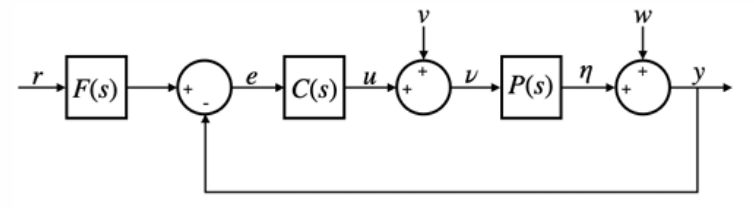
\includegraphics[width=1\linewidth]{W1_control_system.png}
		\caption{Simple unity feedback control loop with reference input $r$}
		\label{fig:W1CS}
	\end{figure}
	
	\subsubsection{Subsystem Definitions and Functional Roles}
	\begin{enumerate}
		\item
		\textbf{Plant $P(s)$}: The physical process or equipment whose dynamic behaviour must be influenced (e.g., an aircraft fuselage, chemical reactor, or DC motor). Its dynamics are dictated by physical laws.
		\item
		\textbf{Controller $C(s)$}: The computational algorithm (implemented in digital microcontrollers, DSPs, or operational amplifiers) that receives the tracking error signal $e(t)$ and calculates the appropriate corrective control command $u(t)$.
		\item
		\textbf{Actuator}: The physical transducer that converts the controller's low-power command signal $u(t)$ into mechanical, hydraulic, or high-power electrical action applied to the plant. Actuators introduce physical limits, such as velocity limits and amplitude saturation.
		\item
		\textbf{Sensor (Measurement Transducer)}: The instrumentation hardware that observes the true plant output variable (e.g., speed, position, pressure) and converts it into an electrical or digital feedback signal. Sensors frequently introduce measurement delays and high-frequency noise.
		\item
		\textbf{Feedforward Pre-Filter $F(s)$}: Positioned before the comparator to filter or shape reference commands prior to error generation. It optimizes transient command tracking without reacting to measurement noise or modifying the closed-loop characteristic poles (commonly set to unity, $F(s) = 1$).
		\item
		\textbf{Summing Junctions and System Signals}:
		\begin{itemize}
			\item
			\textbf{Reference Input $r(t)$}: The desired target setpoint or commanded trajectory.
			\item
			\textbf{Actuating Error $e(t) = r(t) - y(t)$}: The discrepancy between commanded setpoint and actual measured output.
			\item
			\textbf{Input Disturbance $v(t)$}: Unwanted external inputs acting directly on the plant input (e.g., load torque spikes, gradient resistance on a vehicle).
			\item
			\textbf{Output Disturbance / Noise $w(t)$}: High-frequency measurement noise or additive output perturbations corrupting the measured output $y(t)$.
		\end{itemize}
	\end{enumerate}
	\subsubsection{Case Studies in Physical Feedback Systems}
	\begin{itemize}
		\item
		\textbf{DC Motor Speed Control}:
		\begin{itemize}
			\item
			\textit{Plant}: Motor rotor, drive shaft, and mechanical load inertia.
			\item
			\textit{Output $y(t)$}: Rotational speed in RPM or rad/s.
			\item
			\textit{Actuator}: Power amplifier / H-bridge driver delivering motor voltage $u(t)$.
			\item
			\textit{Sensor}: Optical rotary encoder or analog tachometer providing speed feedback.
			\item
			\textit{Controller}: Microcontroller executing a discrete or analog control law (e.g., PID).
			\item
			\textit{Disturbances}: Dynamic changes in load torque or supply voltage fluctuations. When load torque surges, feedback senses the speed drop, increases control voltage, and restores the reference speed.
		\end{itemize}
		\item
		\textbf{Medical Automated Insulin Delivery (Artificial Pancreas)}:
		\begin{itemize}
			\item
			\textit{Plant}: Human physiological blood glucose metabolism.
			\item
			\textit{Actuator}: Electromechanical infusion pump dispensing insulin.
			\item
			\textit{Sensor}: Continuous glucose monitor (CGM) measuring subcutaneous tissue glucose.
			\item
			\textit{Controller}: Embedded algorithm computing micro-bolus insulin delivery rates to regulate blood glucose against carbohydrate meal disturbances.
		\end{itemize}
		\item
		\textbf{Domestic Climate Control (Thermostat)}:
		\begin{itemize}
			\item
			\textit{Plant}: Ambient air within an insulated room.
			\item
			\textit{Actuator}: HVAC furnace, compressor, or heating element.
			\item
			\textit{Sensor}: Thermistor or digital temperature transducer.
			\item
			\textit{Controller}: Bimetallic or digital thermostat switching heating power to hold the temperature at the setpoint regardless of ambient weather variations.
		\end{itemize}
	\end{itemize}
	
	\subsection{Control Paradigms: Feedback vs. Feedforward \& Negative vs. Positive Feedback}
	\subsubsection{Closed-Loop (Feedback) vs. Open-Loop (Feedforward) Control}
	The fundamental distinction lies in whether the control action is driven by measurements of the physical output variable:
	\begin{table}[htbp]
		\centering
		\small
		\caption{Comparison of Control Paradigms: Open-Loop vs. Closed-Loop Control}
		\label{tab:open_vs_closed_loop}
		\begin{tabularx}{\textwidth}{L{0.6} L{1.2} L{1.2}}
			\toprule
			\textbf{Architectural Attribute} & \textbf{Open-Loop (Feedforward) Control} & \textbf{Closed-Loop (Feedback) Control} \\
			\midrule
			\textbf{Feedback Path} & \textbf{Absent}& \textbf{Present}\\
			\addlinespace[4pt]
			\textbf{Disturbance Rejection} & \textbf{Incapable} of counteracting unmodelled disturbances acting on the plant. & \textbf{Actively corrects} for external disturbances by adjusting input based on error. \\
			\addlinespace[4pt]
			\textbf{Sensitivity to Uncertainty} & \textbf{High}; parameter drift, wear, or modelling inaccuracy directly degrades output accuracy. & \textbf{Low}; feedback loop desensitises system performance against internal plant variations. \\
			\addlinespace[4pt]
			\textbf{Stability Risk} & \textbf{No risk} of creating closed-loop instability if the plant itself is stable. & \textbf{Risk of instability}; high gains or phase delays can induce severe oscillations and runaway. \\
			\addlinespace[4pt]
			\textbf{Sensor Noise Sensitivity} & \textbf{Immune}; does not measure output, so no measurement noise enters the loop. & \textbf{Vulnerable}; high-frequency measurement noise is fed back into the controller. \\
			\addlinespace[4pt]
			\textbf{Design Complexity \& Cost} & \textbf{Low}; simpler hardware and no sensor integration required (e.g., standard timer toaster). & \textbf{High}; requires calibrated sensors, wiring, comparative summing junctions, and tuning. \\
			\bottomrule
		\end{tabularx}
	\end{table}
	\subsubsection{Negative Feedback vs. Positive Feedback}
	\begin{itemize}
		\item
		\textbf{Negative Feedback}: The measured output is \textbf{subtracted} from the command setpoint ($e = r - y$). This subtraction causes control action to oppose any divergence from the reference. If output drifts higher than intended, error becomes negative, reducing control effort and pulling the system back to equilibrium. Negative feedback provides self-correction, expands system bandwidth, and stabilizes unstable plants.
		\item
		\textbf{Positive Feedback}: The feedback signal is \textbf{added} to the command ($e = r + y$). This reinforces deviations: any minor perturbation is magnified, creating an escalating regenerative cascade. A real life example is the piercing acoustic howl produced when a live microphone is placed close to a public-address loudspeaker (the amplifier self-amplifies background noise until saturation). Outside specialized trigger circuits (e.g., Schmitt triggers), positive feedback is generally avoided in linear control systems.
	\end{itemize}
	
	\subsection{The Three Fundamental Aims of Control Systems}
	All control engineering designs address three overarching functional objectives
	\subsubsection{Stabilisation}
	Stabilisation is the primary, non-negotiable objective of control design: an unstable system cannot be operated safely. Many physical processes are open-loop unstable, meaning their unforced response grows exponentially and unbounded when subjected to infinitesimal perturbations.
	\begin{itemize}
		\item
		\textbf{Mathematical Objective}: Place all closed-loop characteristic poles strictly inside the stable region (the open left-half complex plane, OLHP) via feedback control laws.
		\item
		\textbf{Physical Example}: An inverted pendulum or a Segway personal transporter. Without active sensing and automatic motor torque adjustment, gravitational torque accelerates the vehicle into a fall. Feedback sensing of chassis tilt angle and angular rate dynamically applies drive wheel acceleration to maintain upright balance.
	\end{itemize}
	\subsubsection{Regulation}
	Regulation focuses on \textbf{maintaining the system output at a fixed, constant setpoint} despite persistent external load disturbances or internal environmental variations.
	\begin{itemize}
		\item
		\textbf{Mathematical Objective}: Minimise the sensitivity transfer function to ensure the steady-state deviation caused by disturbance inputs approaches zero ($y(t) \to r_{\text{const}}$ as $t \to \infty$).
		\item
		\textbf{Physical Examples}:
		\begin{itemize}
			\item
			\textit{Automotive Cruise Control}: Maintaining vehicle speed at exactly $100\text{ km/h}$ despite changing hill gradients (gravity disturbance) and aerodynamic drag variations.
			\item
			\textit{DC Power Supply Regulation}: Maintaining an output terminal voltage despite heavy step fluctuations in load current drawn by downstream electronics.
		\end{itemize}
	\end{itemize}
	\subsubsection{Reference Tracking}
	Reference tracking requires the output $y(t)$ to accurately follow a \textbf{time-varying reference trajectory} $r(t)$ over time. Tracking encompasses regulation as a special case where $r(t)$ is constant. Reference tracking requires balancing two complementary performance regimes:
	\begin{enumerate}
		\item
		\textbf{Transient Performance}: How rapidly and smoothly the system maneuvers immediately following a reference change. This requires fast rise time, well-damped oscillations, and minimal overshoot.
		\item
		\textbf{Steady-State Accuracy}: How closely the output matches the reference as transients decay to zero ($t \to \infty$). For step commands, this entails zero steady-state error ($e_{ss} = 0$), often requiring integral control action in the forward loop.
	\end{enumerate}
	\begin{itemize}
		\item
		\textbf{Physical Examples}:
		\begin{itemize}
			\item
			\textit{Passenger Elevator}: When commanded to move to an upper floor, the cabin must accelerate and travel quickly (fast transient response), decelerate smoothly without overshooting past the floor level (passenger safety/comfort), and stop flush with the landing ($e_{ss} = 0$).
			\item
			\textit{Audio Loudspeaker}: The speaker cone displacement must track dynamic multi-frequency audio voltage waveforms with high fidelity and negligible phase distortion.
		\end{itemize}
	\end{itemize}
	\subsection{Inherent Design Trade-Offs}
	Control engineering is fundamentally an exercise in managing conflicting goals:
	\begin{itemize}
		\item
		Increasing controller gain speeds up response time ($T_r$ decreases) but typically increases overshoot ($M_p$) and reduces stability margins.
		\item
		Aggressive transient tracking demands high actuator control authority, risking physical actuator saturation and exciting unmodelled high-frequency structural resonances.
		\item
		Wide closed-loop bandwidth improves tracking response speed but allows high-frequency sensor noise to enter the loop and vibrate actuators.
	\end{itemize}
	
	\subsection{Quantitative Performance Specifications}
	To quantitatively evaluate control systems against design requirements, engineers apply standard benchmark test signals. The most widely utilized benchmark is the \textbf{unit step input} ($r(t) = 1 \cdot u(t) \implies R(s) = \frac{1}{s}$), representing an abrupt, persistent setpoint change.
	The resulting time response illustrates both transient behaviour and steady-state accuracy.
	\subsubsection{Formal Definitions and Mathematical Formulations}
	For a second order closed loop transfer function $T(s) = \frac{\omega_n^2}{s^2 + 2\zeta\omega_n s + \omega_n^2}$, the general placement of poles are:
	\[
	s_{1,2} = -\zeta\omega_n \pm j\omega_n\sqrt{1 - \zeta^2} = -\sigma \pm j\omega_d
	\]
	\paragraph{Rise Time ($T_r$)}
	\begin{itemize}
		\item
		\textbf{Definition}: The time required for the response to rise from a lower threshold to an upper threshold of its final steady-state value.
		\item
		\textbf{Standard Conventions}: Measured from \textbf{$10\%$ to $90\%$ of $c_{\text{final}}$} for overdamped and general systems, and occasionally $0\%$ to $100\%$ for underdamped second-order systems.
		\item
		\textbf{Physical Meaning}: Quantifies response speed. A small $T_r$ corresponds to rapid tracking, but excessive speed demands heavy control effort and risks high overshoot.
		\item
		\textbf{Analytical Expressions}:
		\begin{itemize}
			\item
			\textit{First-Order System} ($G(s) = \frac{a}{s+a}$ with time constant $\tau = \frac{1}{a}$): \[
			T_r = \frac{\ln(0.9) - \ln(0.1)}{a} \approx \frac{2.2}{a} = 2.2\tau
			\]
			\item
			\textit{Second-Order Underdamped System} ($\zeta \in [0.3, 0.8]$ approximation): \[
			T_r \approx \frac{2.16\zeta + 0.6}{\omega_n} \quad \text{or crudely} \quad T_r \approx \frac{1.8}{\omega_n}
			\]
		\end{itemize}
	\end{itemize}
	\paragraph{Peak Time ($T_p$)}
	\begin{itemize}
		\item
		\textbf{Definition}: The exact time instant at which the step response reaches its \textbf{first, maximum peak value} ($c_{\text{max}}$).
		\item
		\textbf{Analytical Derivation}: For a standard prototype second-order underdamped system with closed-loop transfer function $T(s) = \frac{\omega_n^2}{s^2 + 2\zeta\omega_n s + \omega_n^2}$, the peak occurs where $\frac{dc(t)}{dt} = 0$: \[
		T_p = \frac{\pi}{\omega_n \sqrt{1 - \zeta^2}} = \frac{\pi}{\omega_d}
		\] where $\zeta$ is the damping ratio ($0 \le \zeta < 1$) and $\omega_d = \omega_n \sqrt{1 - \zeta^2}$ is the damped natural frequency.
		\item
		\textbf{Physical Meaning}: $T_p$ is inversely proportional to the imaginary part of the dominant complex poles ($\omega_d$). Moving poles vertically upwards on the $s$-plane shortens $T_p$ without changing the settling envelope.
	\end{itemize}
	\paragraph{Percentage Overshoot ($M_p$ or $\%OS$)}
	\begin{itemize}
		\item
		\textbf{Definition}: The maximum amount by which the transient response waveform overshoots its steady-state value, normalized as a percentage of the steady-state value: \[
		M_p \equiv \frac{c_{\text{max}} - c_{\text{final}}}{c_{\text{final}}} \times 100\%
		\]
		\item
		\textbf{Analytical Derivation}: Evaluating the time-domain response $c(t)$ at $t = T_p$ yields: \[
		M_p = e^{-( \frac{\zeta \pi}{\sqrt{1 - \zeta^2}} )} \times 100\%
		\]
		\item
		\textbf{Damping Ratio Inversion}: Given a percentage overshoot design specification, the required damping ratio $\zeta$ is calculated by: \[
		\zeta = \frac{-\ln(M_p / 100)}{\sqrt{\pi^2 + \ln^2(M_p / 100)}}
		\]
		\item
		\textbf{Physical Meaning}: Overshoot depends solely on the damping ratio $\zeta$ and indicates relative stability. On the $s$-plane, lines of constant radial angle $\theta = \arccos(\zeta)$ represent contours of constant overshoot. Excessive overshoot is prohibited in systems where exceeding nominal limits causes damage (e.g., automated pharmaceutical dosing or precision robotics).
	\end{itemize}
	\paragraph{Settling Time ($T_s$)}
	\begin{itemize}
		\item
		\textbf{Definition}: The time required for the response curve to enter and \textbf{permanently remain within an error tolerance band} around the steady-state value $c_{\text{final}}$.
		\item
		\textbf{Tolerance Bands}: Industrial standards specify either a \textbf{$\pm 2\%$ band} or a \textbf{$\pm 5\%$ band}.
		\item
		\textbf{Analytical Derivation}: The exponential decay envelope of an underdamped second-order response is governed by $e^{-\zeta \omega_n t} = e^{-\sigma t}$, where $\sigma = \zeta \omega_n$ is the real part of the complex conjugate poles.
		\begin{itemize}
			\item
			\textit{For the $2\%$ criterion} ($e^{-\sigma T_s} \le 0.02 \implies -\sigma T_s \approx \ln(0.02) \approx -3.91$): \[
			T_s \approx \frac{4}{\sigma} = \frac{4}{\zeta \omega_n}
			\]
			\item
			\textit{For the $5\%$ criterion} ($e^{-\sigma T_s} \le 0.05 \implies -\sigma T_s \approx \ln(0.05) \approx -2.996$): \[
			T_s \approx \frac{3}{\sigma} = \frac{3}{\zeta \omega_n}
			\]
		\end{itemize}
		\item
		\textbf{Physical Meaning}: Settling time is inversely proportional to the real distance of the poles from the imaginary axis ($\sigma$). Moving poles farther to the left in the OLHP speeds up decay and reduces settling time.
	\end{itemize}
	\paragraph{Steady-State Value ($c_{\text{final}}$) and Steady-State Error ($e_{ss}$)}
	\begin{itemize}
		\item
		\textbf{Steady-State Value}: The asymptotic level reached by the output as time approaches infinity after all transient modes have decayed: \[
		c_{\text{final}} = \lim_{t \to \infty} c(t)
		\]
		\item
		\textbf{Steady-State Error ($e_{ss}$)}: The difference between the commanded reference input and the final output value: \[
		e_{ss} \equiv \lim_{t \to \infty} e(t) = \lim_{t \to \infty} [r(t) - c(t)]
		\]
		\item
		\textbf{Evaluating $e_{ss}$ via the Final Value Theorem}: \[
		e_{ss} = \lim_{s \to 0} s E(s) = \lim_{s \to 0} \frac{s R(s)}{1 + P(s)C(s)}
		\] provided that all poles of $sE(s)$ reside strictly in the open left-half plane. For a unit step input ($R(s) = 1/s$), achieving $e_{ss} = 0$ requires the open-loop forward path $P(s)C(s)$ to contain at least one pure pole at the origin (an integrator, $s=0$), representing a Type-1 system.
	\end{itemize}
	
	\subsection{Comprehensive Review Matrix}
	This reference table summarizes the key subsystems, objectives, and quantitative metrics.
	\begin{center}\small\begin{tabularx}{\textwidth}{*{2}{Y}}
			\toprule
			\textbf{Component / Metric} & \textbf{Mathematical Expression / Symbol} \\
			\midrule
			\textbf{Plant} & $P(s) = \frac{Y(s)}{U(s)}$ \\
			\textbf{Controller} & $C(s)$ \\
			\textbf{Actuator} & Dynamic block / saturation limits \\
			\textbf{Sensor} & Measurement transducer \\
			\textbf{Pre-filter} & $F(s)$ (often $F(s)=1$) \\
			\textbf{Stabilisation} & Poles of $T(s) \in \text{OLHP}$ \\
			\textbf{Regulation} & $\lim_{t \to \infty} y(t) = r_0$ despite $v(t)$ \\
			\textbf{Tracking} & $y(t) \to r(t)$ as $t \to \infty$ \\
			\textbf{Rise Time} & $T_r \approx \frac{2.2}{a}$ (1st) or $\frac{2.16\zeta+0.6}{\omega_n}$ \\
			\textbf{Peak Time} & $T_p = \frac{\pi}{\omega_n \sqrt{1 - \zeta^2}} = \frac{\pi}{\omega_d}$ \\
			\textbf{Overshoot} & $M_p = e^{-(\frac{\zeta \pi}{\sqrt{1-\zeta^2}})} \times 100\%$ \\
			\textbf{Settling Time} & $T_s \approx \frac{4}{\zeta \omega_n} = \frac{4}{\sigma}$ ($2\%$ band) \\
			\textbf{Steady-State Error} & $e_{ss} = \lim_{s \to 0} \frac{s R(s)}{1 + P(s)C(s)}$ \\
			\bottomrule
	\end{tabularx}\end{center}
	
	\subsection{Interactive Self-Study Questions}
	Test your understanding of the Week 1 core concepts:
	\begin{enumerate}
		\item
		\textbf{Poles vs. Zeros}: Why does an LTI continuous-time system become unstable if a pole lies in the right-half plane, and does having a zero in the right-half plane cause the system's unforced response to blow up?
		\item
		\textbf{Negative vs Positive Feedback}: Why does positive feedback lead to signal saturation or instability, while negative feedback stabilizes the output?
		\item
		\textbf{Step Response Trade-offs}: If a customer requires reducing the settling time $T_s$ by half while keeping percentage overshoot $M_p$ strictly constant, how must the poles of the second-order system move in the complex $s$-plane?
	\end{enumerate}
	
	\newpage
	\section{System Modelling}

	
	\subsection{Master Checklist: Week 2 Core Competencies}
	\begin{itemize}
		\item[$\square$]
		\textbf{The Purpose \& Hierarchy of Modelling}: Explain why mathematical models are necessary in control engineering and outline the progression from a real physical plant to an idealised physical model, a mathematical model, and a simplified linearised model.
		\item[$\square$]
		\textbf{Model Uncertainty}: Describe why all models are approximations of reality and how model uncertainty influences controller design.
		\item[$\square$]
		\textbf{Analytical (First-Principles) Modelling}: Derive ordinary differential equations (ODEs) and transfer functions using fundamental conservation and physical laws (Newton’s laws, Kirchhoff’s voltage and current laws).
		\item[$\square$]
		\textbf{System Order \& Energy Storage Elements}: State the physical relationship between the order of a transfer function's denominator polynomial and the number of independent energy storage elements in the system.
		\item[$\square$]
		\textbf{Mechanical \& Electrical Analogies}: Map the mathematical equivalence between mechanical components (mass, damper, spring) and electrical components (inductor, resistor, capacitor).
		\item[$\square$]
		\textbf{Linearisation of Nonlinear Systems}: Formulate the first-order Taylor series approximation to linearise a nonlinear differential equation around a steady-state equilibrium operating point.
		\item[$\square$]
		\textbf{Empirical Modelling (System Identification)}: Define the "black-box" identification approach and state when it is preferred over analytical modelling.
		\item[$\square$]
		\textbf{The Three-Step Identification Workflow}: Master the three systematic steps: (1) Model Structure Selection, (2) Informative Input Excitation, and (3) Parameter Estimation.
		\item[$\square$]
		\textbf{Informative Test Signals}: Explain why step inputs, impulses, and sinusoidal frequency sweeps are selected to reveal natural frequencies, damping, time constants, and DC gains.
		\item[$\square$]
		\textbf{Parameter Estimation \& Optimization}: Formulate the sum-of-squared-errors (least-squares) objective function used to optimise model parameter vectors.
		\item[$\square$]
		\textbf{Overfitting \& Model Validation}: Explain the danger of model overfitting to measurement noise and formulate the procedure for validating models against separate, independent test data.
	\end{itemize}
	
	\subsection{Why Model? The Modelling Hierarchy \& Uncertainty}
	\subsubsection{The Role of Models in Control Design}
	Control design is carried out primarily on a mathematical model rather than directly on physical hardware. Operating directly on physical hardware during early design iterations can be costly, time-consuming, or hazardous. A mathematical model allows engineers to:
	\begin{enumerate}
		\item
		\textbf{Simulate dynamic behaviour} under diverse operating regimes and extreme conditions without risking physical damage.
		\item
		\textbf{Synthesise controllers analytically} to meet exact performance and stability specifications before implementation.
		\item
		\textbf{Generalise past observations} to predict system responses to previously unencountered inputs and environmental disturbances.
	\end{enumerate}
	\subsubsection{The Hierarchy of System Models}
	Modelling involves progressing through four distinct levels of abstraction:
	
	\begin{itemize}
		\item Real Physical System
		\item Idealized Physical System
		\item Mathematical Model
		\item Simplified LTI Model
	\end{itemize}
	
	\subsubsection{Model Uncertainty}
	A central principle emphasised in control theory is that \textbf{"all models are approximations of reality"}. No mathematical model represents the real physical plant with complete precision.
	\begin{itemize}
		\item
		\textbf{Sources of Uncertainty}: Physical parameter drift (e.g., thermal changes in resistance, wear in mechanical dampers), unmodelled high-frequency dynamics (e.g., structural flexibility, sensor delays), and neglected nonlinearities (e.g., Coulomb friction, actuator saturation).
		\item
		\textbf{Engineering Implication}: A model must capture the \textit{dominant} dynamics necessary for feedback control while remaining analytically tractable. Feedback controllers must then be designed to remain robust against the inevitable residual model uncertainty.
	\end{itemize}
	
	\subsection{Analytical Modelling (First-Principles Derivation)}
	Analytical modelling relies on established scientific and physical laws to construct differential equations directly from the interconnection of idealised physical components.
	\subsubsection{Governing Physical Laws Across Engineering Domains}
	When constructing models from first principles, engineers sum across energy storage and dissipative mechanisms:
	\begin{itemize}
		\item
		\textbf{Mechanical Translational Systems}: Newton’s Second Law of Motion: \[
		\sum F_{\text{ext}}(t) = m a(t) = m \frac{d^2 x(t)}{dt^2}
		\] where forces originate from applied actuators, Hooke's law for springs ($F_k = k x$), and viscous damping forces ($F_b = c \dot{x}$).
		\item
		\textbf{Mechanical Rotational Systems}: Newton's Rotational Analogue: \[
		\sum T_{\text{ext}}(t) = J \alpha(t) = J \frac{d^2 \theta(t)}{dt^2}
		\] balancing inertia torque $J \ddot{\theta}$, torsional stiffness $k \theta$, and viscous rotational damping $B \dot{\theta}$.
		\item
		\textbf{Electrical Networks}: Kirchhoff’s Laws:
		\begin{itemize}
			\item
			\textit{Kirchhoff's Voltage Law (KVL)}
			\item
			\textit{Kirchhoff's Current Law (KCL)}
		\end{itemize}
	\end{itemize}
	
	\subsubsection{Benchmark Analytical Model 1: Translational Mass-Spring-Damper}
	Consider a classic second-order mechanical system consisting of a rigid mass $m$, a viscous friction damper with damping coefficient $c$, and a linear restoring spring with spring constant $k$, subjected to an external driving force $u(t)$:
	
	\begin{figure}[H]
		\centering
		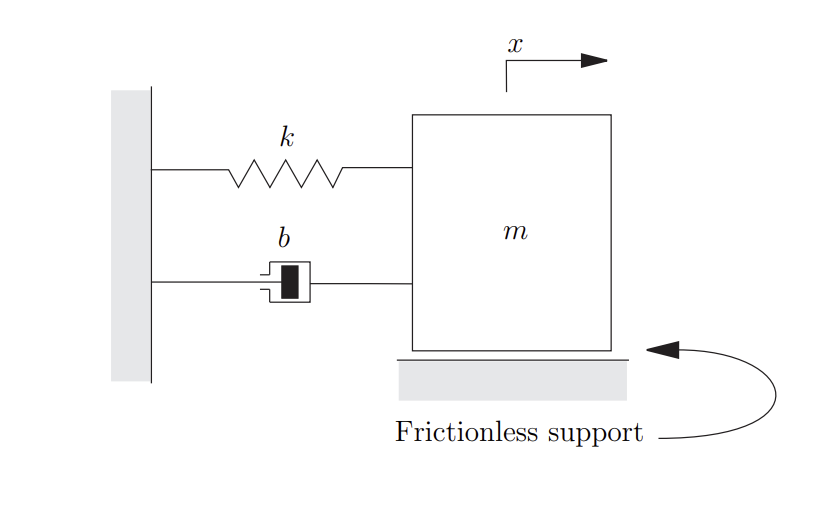
\includegraphics[height=5cm]{W2_mass_damper.png}
		\caption{Second-order mechanical system}
		\label{fig:W2MD}
	\end{figure}
	
	\begin{enumerate}
		\item
		\textbf{Free-Body Dynamic Force Balance}: Applying Newton's second law along the horizontal axis: \[
		u(t) - F_{\text{damper}}(t) - F_{\text{spring}}(t) = m \frac{d^2 y(t)}{dt^2}
		\] Substituting the constituent equations $F_{\text{damper}}(t) = c \dot{y}(t)$ and $F_{\text{spring}}(t) = k y(t)$: \[
		m \frac{d^2 y(t)}{dt^2} + c \frac{dy(t)}{dt} + k y(t) = u(t)
		\]
		\item
		\textbf{Laplace Transformation}: Taking the unilateral Laplace transform assuming zero initial conditions ($y(0) = \dot{y}(0) = 0$): \[
		\left( m s^2 + c s + k \right) Y(s) = U(s)
		\]
		\item
		\textbf{Transfer Function Formulation}: \[
		G(s) = \frac{Y(s)}{U(s)} = \frac{1}{m s^2 + c s + k} = \frac{\frac{1}{m}}{s^2 + \left(\frac{c}{m}\right)s + \left(\frac{k}{m}\right)}
		\] Comparing this directly with the standard prototype second-order characteristic denominator $s^2 + 2\zeta\omega_n s + \omega_n^2$ yields the fundamental system parameters: \[
		\omega_n = \sqrt{\frac{k}{m}} \quad \text{(Undamped Natural Frequency)}
		\] \[
		2\zeta\omega_n = \frac{c}{m} \implies \zeta = \frac{c}{2\sqrt{km}} \quad \text{(Damping Ratio)}
		\] This analytical model provides immediate physical insights into parameter influences:
		\begin{itemize}
			\item
			\textbf{Increasing mass $m$} decreases $\omega_n$, making the system response slower and more sluggish.
			\item
			\textbf{Increasing damping coefficient $c$} increases $\zeta$, attenuating transient oscillations and reducing overshoot.
			\item
			\textbf{Increasing stiffness $k$} increases natural frequency $\omega_n$, stiffening the response and speeding up initial movement.
		\end{itemize}
	\end{enumerate}
	
	\subsubsection{Benchmark Analytical Model 2: Series RLC Circuit}
	Consider a series electrical network comprising a resistor $R$, an inductor $L$, and a capacitor $C$ driven by an input voltage source $v(t)$, where the output is the capacitor voltage $v_C(t)$:
	
	\begin{figure}[H]
		\centering
		\begin{circuitikz}[american, scale=0.75, transform shape]
			\draw (0,0) 
			% Voltage Source on the left vertical leg
			to[sV, l=$v(t)$] (0,3) 
			% Resistor, Inductor, and Capacitor in series along the top rail
			to[R, l=$R$] (3,3) 
			to[L, l=$L$] (6,3) 
			to[C, l=$C$] (9,3) 
			% Return path along the right vertical and bottom rails
			to[short] (9,0) 
			to[short] (0,0);
		\end{circuitikz}
		\caption{RLC Circuit}
	\end{figure}
	
	
	
	\begin{enumerate}
		\item
		\textbf{Integro-Differential Equation via KVL}: Summing the voltage drops around the loop: \[
		L \frac{di(t)}{dt} + R i(t) + v_C(t) = v(t)
		\] Using the capacitor constitutive relation $i(t) = C \frac{dv_C(t)}{dt}$: \[
		L C \frac{d^2 v_C(t)}{dt^2} + R C \frac{dv_C(t)}{dt} + v_C(t) = v(t)
		\]
		\item
		\textbf{Transfer Function}: Applying the Laplace transform with zero initial conditions: \[
		(L C s^2 + R C s + 1) V_C(s) = V(s)
		\] \[
		G(s) = \frac{V_C(s)}{V(s)} = \frac{\frac{1}{LC}}{s^2 + \left(\frac{R}{L}\right)s + \frac{1}{LC}}
		\] Here, the natural frequency and damping ratio map directly to electrical quantities: \[
		\omega_n = \frac{1}{\sqrt{LC}}, \qquad \zeta = \frac{R}{2}\sqrt{\frac{C}{L}}
		\]
	\end{enumerate}
	
	\subsubsection{Energy Storage Elements and Transfer Function Order}
	A fundamental principle highlighted in Week 2 is the relationship between the physical components and the mathematical order of the model:
	\begin{itemize}
		\item
		\textbf{The Rule of System Order}: The \textbf{order of the transfer function} (the highest power of $s$ in the characteristic denominator polynomial) equals the \textbf{number of independent energy storage elements} present in the physical system.
		\item
		\textbf{Energy Storage Elements}:
		\begin{itemize}
			\item
			\textit{Translational Mechanical}: Masses (kinetic energy $E_k = \frac{1}{2}m v^2$) and Springs (potential strain energy $E_p = \frac{1}{2}k x^2$).
			\item
			\textit{Rotational Mechanical}: Rotor inertias ($E_k = \frac{1}{2}J \omega^2$) and Torsional shafts ($E_p = \frac{1}{2}K \theta^2$).
			\item
			\textit{Electrical}: Inductors (magnetic field energy $E_m = \frac{1}{2}L i^2$) and Capacitors (electric field energy $E_e = \frac{1}{2}C v^2$).
			\item
			\textit{Thermal \& Fluid}: Thermal capacitances (stored heat $m c_p \Delta T$) and Fluid reservoirs/tanks (potential hydrostatic energy).
		\end{itemize}
		\item
		\textbf{Energy Dissipating Elements}: Dampers (viscous friction) and Resistors do not store energy; they dissipate energy as heat and contribute to the real parts of the system poles (damping) without increasing the system order.
	\end{itemize}
	\subsubsection{Mechanical–Electrical Physical Analogies (Series / Force–Voltage Analogue)}
	Because both mechanical and electrical systems obey analogous second-order differential equations, engineers frequently exploit direct mathematical analogies:
	\begin{center}\small\begin{tabularx}{\textwidth}{*{4}{Y}}
			\toprule
			\textbf{Mechanical Component (Translational)} & \textbf{Constitutive Relation} & \textbf{Electrical Equivalent (Series Mesh)} & \textbf{Constitutive Relation} \\
			\midrule
			\textbf{Applied Force $F(t)$} & Driving input & \textbf{Voltage $v(t)$} & Driving potential \\
			\textbf{Velocity $v(t) = \dot{x}(t)$} & Dynamic flow & \textbf{Current $i(t)$} & Charge flow \\
			\textbf{Mass $M$} (Kinetic energy) & $F = M \frac{dv}{dt}$ & \textbf{Inductance $L$} (Magnetic energy) & $v = L \frac{di}{dt}$ \\
			\textbf{Damper $c$ or $f_v$} (Dissipation) & $F = c v$ & \textbf{Resistance $R$} (Thermal dissipation) & $v = R i$ \\
			\textbf{Spring $k$} (Potential energy) & $F = k \int v\, dt$ & \textbf{Capacitance $1/C$} (Elastance) & $v = \frac{1}{C}\int i\, dt$ \\
			\bottomrule
	\end{tabularx}\end{center}
	
	\subsubsection{Linearisation Around an Equilibrium Operating Point}
	Most physical systems exhibit nonlinear dynamics (e.g., aerodynamic drag proportional to $v^2$, gravitational torque on a pendulum $mgl \sin\theta$, or fluid flow through orifices proportional to $\sqrt{\Delta P}$). Linear control techniques (Laplace transforms, frequency response, root locus) require linear time-invariant approximations near a nominal operating point.
	\paragraph{The Mathematical Linearisation Procedure}
	\begin{enumerate}
		\item
		\textbf{Define the Equilibrium Point}: Consider an autonomous or controlled nonlinear differential equation $\dot{x}(t) = f(x(t), u(t))$. An equilibrium operating point $(x_e, u_e)$ satisfies the steady-state zero-derivative condition: \[
		f(x_e, u_e) = 0
		\]
		\item
		\textbf{Define Deviation Variables (Perturbations)}: Let small perturbations about the equilibrium be defined as: \[
		\delta x(t) = x(t) - x_e, \qquad \delta u(t) = u(t) - u_e
		\]
		\item
		\textbf{Perform First-Order Taylor Series Expansion}: Expanding $f(x, u)$ around $(x_e, u_e)$: \[
		\dot{x} = \frac{d(x_e + \delta x)}{dt} = \dot{\delta x} = f(x_e, u_e) + \left. \frac{\partial f}{\partial x} \right|_{(x_e, u_e)} \delta x(t) + \left. \frac{\partial f}{\partial u} \right|_{(x_e, u_e)} \delta u(t) + \text{H.O.T.}
		\]
		\item
		\textbf{Neglect Higher-Order Terms (H.O.T.)}: Because $f(x_e, u_e) = 0$, and assuming perturbations $\delta x$ and $\delta u$ remain small, higher-order powers ($\delta x^2, \delta x \delta u$, etc.) are neglected: \[
		\dot{\delta x}(t) \approx A \delta x(t) + B \delta u(t)
		\] where the constant Jacobian matrices are: \[
		A = \left. \frac{\partial f}{\partial x} \right|_{(x_e, u_e)}, \qquad B = \left. \frac{\partial f}{\partial u} \right|_{(x_e, u_e)}
		\] Taking the Laplace transform of this perturbation equation yields a valid local LTI transfer function relating $\delta X(s)$ to $\delta U(s)$.
	\end{enumerate}
	
	\subsection{Empirical Modelling (System Identification from Data)}
	\subsubsection{The "Black-Box" System Identification Paradigm}
	When systems involve complex, distributed, or poorly understood physics (e.g., biological metabolisms, industrial chemical distillation columns, aerodynamic turbulence, or soft robotics), deriving exact equations from first principles is difficult or impossible.
	In such cases, the system is treated as a \textbf{"black box"}:
	\begin{figure}[H]
		\centering
		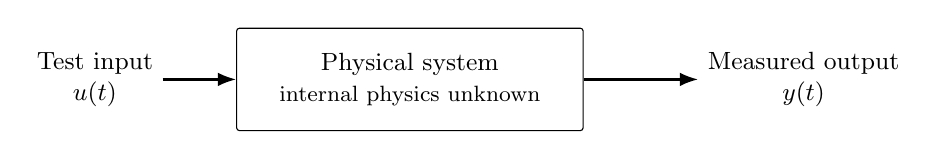
\begin{tikzpicture}[>=Latex, every node/.style={font=\small}]
			\node[align=center] (u) at (-4,0) {Test input\\$u(t)$};
			\node[ctlwide,minimum width=4.4cm,minimum height=13mm] (sys) at (0,0) {Physical system\\\footnotesize internal physics unknown};
			\node[align=center] (y) at (5,0) {Measured output\\$y(t)$};
			\draw[signal] (u.east) -- (sys.west);
			\draw[signal] (sys.east) -- (y.west);
		\end{tikzpicture}
		\caption{Black-box setup for empirical system identification.}
		\label{fig:black-box-identification}
	\end{figure}
	By applying known input signals $u(t)$ and logging the resulting output response data $y(t)$, an empirical model is fitted to match the observed input-output behaviour.
	
	\subsubsection{The Three Systematic Steps of System Identification}
	System identification follows a three-step methodology:
	\begin{figure}[H]
		\centering
		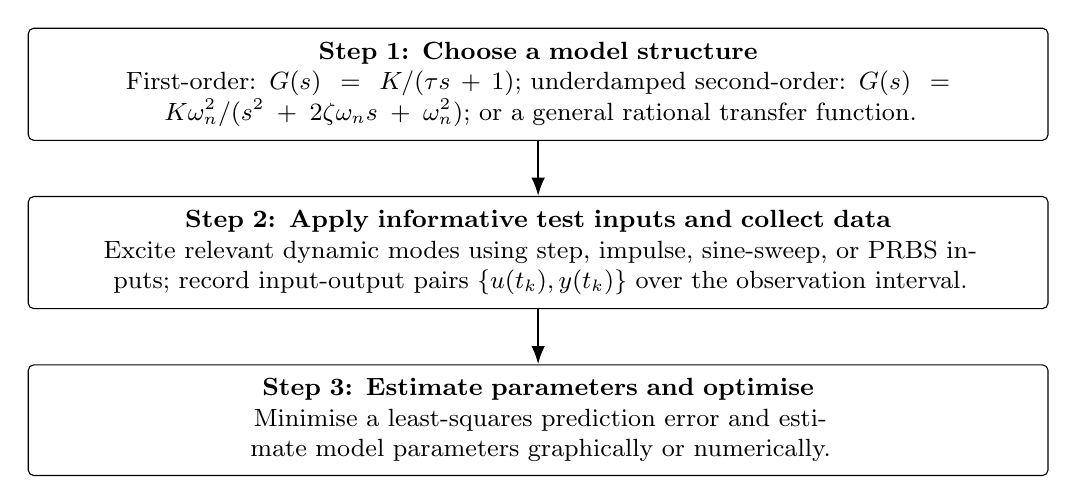
\begin{tikzpicture}[node distance=7mm,>=Latex,every node/.style={font=\small}]
			\node[flowbox] (s1) {\textbf{Step 1: Choose a model structure}\\
				First-order: $G(s)=K/(\tau s+1)$; underdamped second-order: $G(s)=K\omega_n^2/(s^2+2\zeta\omega_n s+\omega_n^2)$; or a general rational transfer function.};
			\node[flowbox,below=of s1] (s2) {\textbf{Step 2: Apply informative test inputs and collect data}\\
				Excite relevant dynamic modes using step, impulse, sine-sweep, or PRBS inputs; record input-output pairs $\{u(t_k),y(t_k)\}$ over the observation interval.};
			\node[flowbox,below=of s2] (s3) {\textbf{Step 3: Estimate parameters and optimise}\\
				Minimise a least-squares prediction error and estimate model parameters graphically or numerically.};
			\draw[flowarrow] (s1) -- (s2);
			\draw[flowarrow] (s2) -- (s3);
		\end{tikzpicture}
		\caption{Three-step workflow for empirical system identification.}
		\label{fig:system-id-workflow}
	\end{figure}
	\paragraph{Step 1: Choose a Model Structure}
	The designer decides on the mathematical structure and order of the candidate model prior to fitting:
	\begin{itemize}
		\item
		\textbf{Prior Insight Selection}: If physical insight indicates a single dominant thermal lag or a spring-mass resonance, a specific first-order or second-order structure is chosen.
		\item
		\textbf{Generic Rational Transfer Function}: \[
		G(s) = \frac{b_m s^m + b_{m-1} s^{m-1} + \dots + b_0}{s^n + a_{n-1} s^{n-1} + \dots + a_0}
		\]
		\item
		\textbf{First-Order Model}: \[
		G(s) = \frac{K}{\tau s + 1}
		\] governed by static DC gain $K$ and time constant $\tau$.
	\end{itemize}
	\paragraph{Step 2: Apply Informative Test Inputs and Collect Output Data}
	To identify a model reliably, the test input signal must \textbf{persistently excite} the system across the frequency spectrum where control will take place:
	\begin{itemize}
		\item
		\textbf{Step Input ($u(t) = U_0 \cdot \mathbf{1}(t)$)}: The most common industrial test (bump test). Reveals steady-state DC gain, dominant time constants, presence of pure time delays, and oscillatory damping behaviour.
		\item
		\textbf{Impulse Input}: Provides the system’s natural transient modes directly in the time domain.
		\item
		\textbf{Sinusoidal Inputs / Sine Frequency Sweeps}: Tests the system at discrete frequencies $\omega$ to generate empirical Bode gain and phase plots directly.
	\end{itemize}
	\paragraph{Step 3: Estimate Model Parameters (Least-Squares Optimization)}
	The model parameters (collected in vector $\theta$) are tuned so that the predicted model output $y_\theta(t_k)$ tracks the measured experimental output $y(t_k)$ as closely as possible.
	\begin{itemize}
		\item
		\textbf{Sum of Squared Errors (Least-Squares Criterion)}: The standard optimization problem minimizes the quadratic prediction error over $N$ sampled discrete-time measurements: \[
		J(\theta) = \sum_{k=1}^{N} \left[ y(t_k) - y_\theta(t_k) \right]^2
		\] where:
		\begin{itemize}
			\item
			$y(t_k)$ is the true measured output at sampling instant $t_k$.
			\item
			$y_\theta(t_k)$ is the simulated output produced by the candidate model transfer function $G(s; \theta)$ driven by the recorded input $u(t_k)$.
		\end{itemize}
		\item
		\textbf{Solution Methods}: Linear least-squares (via normal equations) for linear regression structures, or nonlinear least-squares algorithms (e.g., Levenberg-Marquardt, gradient descent) implemented in computational tools.
	\end{itemize}
	
	\subsubsection{Graphical Parameter Extraction from Step Response Data (FOTD / Bump Test)}
	For monotone, non-oscillatory processes, empirical models are frequently extracted directly from step response curves. Consider a First-Order with Time Delay (FOTD) model: \[
	G(s) = \frac{K}{\tau s + 1} e^{-Ls}
	\] where $K$ is the DC gain, $\tau$ is the time constant, and $L$ is the apparent physical transport lag/dead time.
	
	\begin{enumerate}
		\item
		\textbf{Steady-State DC Gain ($K$)}: Calculate the ratio of the total change in output to the magnitude of the input step change $\Delta u$: \[
		K = \frac{\Delta y_{\text{final}}}{\Delta u} = \frac{y(\infty) - y(0)}{u(\infty) - u(0)}
		\]
		\item
		\textbf{Apparent Time Delay ($L$)}: Draw a tangent line through the steepest inflection point of the step response curve. The time coordinate where this tangent intersects the initial baseline defines the apparent dead time $L$.
		\item
		\textbf{Time Constant ($\tau$) via the $63.2\%$ Method}: For a first-order system, the output reaches $1 - e^{-1} \approx 63.2\%$ of its net change after one time constant has elapsed past the delay: \[
		y(T_{63}) - y(0) = 0.632 \cdot \Delta y_{\text{final}} \implies \tau = T_{63} - L
		\]
	\end{enumerate}
	
	\subsubsection{Overfitting, Noise Rejection, and Model Validation}
	\paragraph{The Risk of Overfitting}
	When selecting a model structure, a higher-order model (more poles and zeros) can achieve a smaller fitting error on the training dataset. However, this introduces \textbf{overfitting}:
	\begin{itemize}
		\item
		An overly complex model fits the \textbf{high-frequency measurement noise} and transient recording anomalies rather than the underlying physical plant dynamics.
		\item
		Such models generalize poorly, resulting in inaccurate predictions and unstable feedback loops when deployed in real-world environments.
		\item
		\textbf{Rule of Parsimony}: A simpler, lower-order model that captures the dominant time constants and natural frequencies is preferred.
	\end{itemize}
	\paragraph{Model Validation}
	A model must never be evaluated solely on the data used to estimate its parameters.
	\begin{itemize}
		\item
		\textbf{Cross-Validation}: Split the collected experimental data into two distinct subsets:
		\begin{enumerate}
			\item
			\textbf{Estimation (Training) Dataset}: Used to calculate the optimal parameter vector.
			\item
			\textbf{Validation (Test) Dataset}: The model’s simulated output $y_\theta(t)$ is compared against this unseen dataset.
		\end{enumerate}
		\item
		If the model achieves a high fit percentage on the test validation dataset without exhibiting spurious oscillations, it is validated for controller design.
	\end{itemize}
	
	\subsection{Analytical vs. Data-Driven Modeling}
	\begin{center}\small\begin{tabularx}{\textwidth}{*{3}{Y}}
			\toprule
			\textbf{Characteristic} & \textbf{Analytical Modeling (First-Principles)} & \textbf{Empirical Modelling (System Identification)} \\
			\midrule
			\textbf{Foundational Basis} & Universal physical and scientific laws. & Input-output experimental time/frequency measurements. \\
			\textbf{System Knowledge Required} & Complete internal physical architecture and parameter specifications. & Unknown "black box". \\
			\textbf{Parameter Physical Meaning} & High; parameters correspond directly to mass, resistance, volume, etc.. & Low; parameters are mathematical polynomial coefficients or fits. \\
			\textbf{Handling of Unmodelled Physics} & Struggles with complex friction, turbulence, and distributed parasitics. & Naturally captures lumped empirical effects present in the test data. \\
			\textbf{Risk of Overfitting} & None; physical component laws strictly constrain the model structure. & High; overly high polynomial orders fit noise instead of true dynamics. \\
			\textbf{Generalisability} & High; can predict behaviour across varying configurations and sizes. & Limited; accurate primarily near the amplitude and frequency ranges tested. \\
			\bottomrule
	\end{tabularx}\end{center}
	
	\subsection{Interactive Review \& Self-Study Questions}
	Test your understanding of Week 2 concepts:
	\begin{enumerate}
		\item
		\textbf{System Order Deduction}: A hydraulic fluid network contains two fluid reservoirs and three flow-restricting valves. Assuming no pipe elasticity or fluid compressibility, what is the order of the resulting linear differential equation?
		\item
		\textbf{Linearisation Condition}: When linearising a nonlinear model $\dot{x} = f(x, u)$ using Taylor series expansion, what condition must hold for the steady-state nominal operating point $(x_e, u_e)$?
		\item
		\textbf{Data-Driven Model Selection}: Why is choosing a tenth-order transfer function to fit noisy step response data from a DC motor considered poor control engineering practice?
	\end{enumerate}
	
	\newpage
	\section{System Response}

	\subsection{Master Checklist: Week 3 Core Competencies}
	\begin{itemize}
		\item[$\square$]
		\textbf{BIBO Stability vs. Internal Stability}: Define Bounded-Input Bounded-Output (BIBO) stability and internal (asymptotic) stability, and understand why internal stability implies BIBO stability.
		\item[$\square$]
		\textbf{Unstable Pole-Zero Cancellations}: Explain why cancelling an open-loop right-half-plane (RHP) pole with a controller zero conceals an internal instability that diverges under nonzero initial conditions or external disturbances.
		\item[$\square$]
		\textbf{Closed-Loop Characteristic Polynomial}: Formulate the characteristic polynomial for a feedback loop, $a_p(s)a_c(s) + b_p(s)b_c(s) = 0$, and state the necessary and sufficient condition for closed-loop stability.
		\item[$\square$]
		\textbf{$s$-Plane Pole Mapping}: Predict time-domain modal responses from pole coordinates across the open left-half-plane (OLHP), imaginary axis ($j\omega$-axis), and right-half-plane (RHP).
		\item[$\square$]
		\textbf{Dominant Pole Approximation}: Define dominant vs. non-dominant poles and apply the standard \textbf{$5\times$ separation rule-of-thumb} to approximate higher-order dynamics with an equivalent second-order model.
		\item[$\square$]
		\textbf{Effects of Left-Half-Plane Zeros}: Explain how adding a stable zero introduces a derivative-like effect that reduces rise time ($T_r$) but increases percentage overshoot ($M_p$).
		\item[$\square$]
		\textbf{Non-Minimum Phase (RHP) Zeros}: Characterise the physical mechanism behind \textbf{inverse response (initial undershoot)} and identify the fundamental performance limitations imposed by RHP zeros.
		\item[$\square$]
		\textbf{Root Locus Concept}: State the mathematical definition of the root locus as the trajectories of closed-loop poles when loop gain $K$ varies from $0 \to \infty$.
		\item[$\square$]
		\textbf{Angle and Magnitude Conditions}: Derive and evaluate the angle condition ($\angle L(s) = \pm 180^\circ(2k+1)$) and magnitude condition ($K = 1/|L(s)|$) for closed-loop pole locations.
		\item[$\square$]
		\textbf{Root Locus Sketching Rules}: Apply rules for the number of branches, real-axis segments, asymptote centroid ($\sigma_a$) and angles ($\theta_a$), breakaway/break-in points, and $j\omega$-axis crossings.
		\item[$\square$]
		\textbf{High-Gain Stability Limits}: Explain why systems with a pole excess $n - m > 2$ or with RHP zeros become unstable at sufficiently large feedback gains.
	\end{itemize}
	
	\subsection{System Stability: BIBO, Internal Stability, and Hidden Modes}
	\subsubsection{Bounded-Input Bounded-Output (BIBO) Stability}
	A continuous-time linear time-invariant (LTI) system is defined as \textbf{BIBO stable} if every bounded input signal produces a bounded output signal: \[
	\exists , M_u < \infty \text{ such that } |u(t)| \le M_u ; \forall , t \ge 0 \implies \exists , M_y < \infty \text{ such that } |y(t)| \le M_y ; \forall , t \ge 0
	\]
	\begin{itemize}
		\item
		\textbf{Poles in the Open Left-Half-Plane (OLHP)}: An LTI transfer function $G(s) = \frac{b(s)}{a(s)}$ is BIBO stable \textbf{if and only if all poles of $G(s)$ lie strictly in the OLHP} ($\text{Re}(p_i) < 0$).
		\item
		\textbf{Poles on the Imaginary Axis}: Systems with poles on the imaginary axis ($\text{Re}(p_i) = 0$) are \textbf{not} BIBO stable. For example, a pure integrator $G(s) = \frac{1}{s}$ has a pole at $s = 0$. When excited by a bounded unit step input $u(t) = 1(t)$, the resulting output is an unbounded ramp $y(t) = t$, violating BIBO stability. Similarly, simple conjugate poles on the $j\omega$-axis yield an unbounded resonance when excited by a sinusoid matched to that natural frequency.
	\end{itemize}

	\subsubsection{Internal Stability vs. BIBO Stability}
	In state-space and interconnected control loops, input-output behaviour does not always capture the state of every internal component:
	\begin{itemize}
		\item
		\textbf{Internal (Asymptotic) Stability}: For an unforced linear system $\dot{x}(t) = Ax(t)$, the equilibrium $x = 0$ is internally stable if and only if \textbf{all eigenvalues of the system matrix $A$ have strictly negative real parts}. Under this condition, the state vector $x(t)$ decays exponentially to zero from any initial state $x(0)$.
		\item
		\textbf{The Relationship}: Internal stability \textbf{guarantees} BIBO stability. However, BIBO stability does \textbf{not} necessarily guarantee internal stability if pole-zero cancellations occur between open-loop components.
	\end{itemize}
	\subsubsection{The Danger of Unstable Pole-Zero Cancellations}
	A critical design rule in feedback engineering is that \textbf{an unstable plant pole must never be cancelled by a controller zero}.
	Consider a plant with an unstable pole at $s = +1$ and a stabilizing controller attempting to cancel it: \[
	P(s) = \frac{s - 1}{(s + 3)(s - 1)}, \qquad C(s) = 1
	\]
	Algebraically cancelling $(s - 1)$ yields the reference-to-output transfer function: \[
	G(s) = \frac{1}{s + 3}
	\] This transfer function appears stable because its only remaining pole lies at $s = -3$ in the OLHP. However, examining the system's differential equation with a non-zero initial condition $y(0) = y_0$ reveals that the unforced response contains the uncancelled natural mode: \[
	y(t) = \frac{y_0}{4}\left( e^{-3t} + e^{t} \right)
	\] Because of the unstable exponential term $e^t$, any nonzero initial condition or minor disturbance forces the internal state and output to diverge toward infinity. In a unity feedback loop with plant $P(s) = \frac{b_p(s)}{a_p(s)}$ and controller $C(s) = \frac{b_c(s)}{a_c(s)}$, internal stability requires that all roots of the full characteristic polynomial: \[
	\Delta(s) = a_p(s)a_c(s) + b_p(s)b_c(s) = 0
	\] lie strictly in the open left-half-plane. An unstable mode can only be stabilized by using feedback to shift the pole into the left-half-plane, not by mathematical cancellation.
	
	\subsection{Dynamic Geography of the Complex $s$-Plane}
	The location of closed-loop poles $s = \sigma \pm j\omega_d$ determines the natural modes that form the transient response:

\begin{table}[htbp]
	\centering
	\caption{Dynamic Characteristics based on $s$-Plane Pole Locations}
	\label{tab:s_plane_pole_responses}
	\small
	\renewcommand{\arraystretch}{1.3} % Adds vertical padding between rows
	\begin{tabularx}{\textwidth}{L{1} L{1.0} L{1.4} L{0.6}}
		\toprule
		\textbf{$s$-Plane Region} & \textbf{Pole Type} & \textbf{Time-Domain Dynamic Response $y(t)$} & \textbf{Stability} \\
		\midrule
		\textbf{Left Half-Plane} & Complex Conjugates & \textbf{Decaying Oscillations} & Stable \\
		$\text{Re}(s) < 0$ & $\sigma < 0, \omega \neq 0$ & $e^{-\sigma t} \sin(\omega t)$ & \\
		\addlinespace[4pt]
		& Real Negative Axis & \textbf{Pure Exponential Decay} & Stable \\
		& $\sigma < 0, \omega = 0$ & $e^{-\sigma t}$ & \\
		\midrule
		\textbf{Right Half-Plane} & Complex Conjugates & \textbf{Growing Oscillations} & Unstable \\
		$\text{Re}(s) > 0$ & $\sigma > 0, \omega \neq 0$ & $e^{\sigma t} \sin(\omega t)$ & \\
		\addlinespace[4pt]
		& Real Positive Axis & \textbf{Pure Exponential Growth} & Unstable \\
		& $\sigma > 0, \omega = 0$ & $e^{\sigma t}$ & \\
		\midrule
		\textbf{Imaginary Axis} & Pure Imaginary & \textbf{Sustained Oscillations} & Marginally \\
		$\text{Re}(s) = 0$ & $\sigma = 0, \omega \neq 0$ & $\sin(\omega t)$ & Stable \\
		\addlinespace[4pt]
		& Origin & \textbf{Constant Step Output} & Marginally \\
		& $\sigma = 0, \omega = 0$ & $y(t) = C$ (Integrator) & Stable \\
		\bottomrule
	\end{tabularx}
\end{table}

	\subsubsection{Regional Characteristics of the $s$-Plane}
	\begin{enumerate}
		\item
		\textbf{Left-Half-Plane (LHP, $\sigma < 0$)}:
		\begin{itemize}
			\item
			Generates exponentially decaying modes $e^{\sigma t} = e^{-|\sigma|t}$.
			\item
			Moving farther left (increasing $|\sigma|$) accelerates decay, shortens time constants ($\tau = 1/|\sigma|$), and reduces settling time ($T_s \approx 4/|\sigma|$).
		\end{itemize}
		\item
		\textbf{Right-Half-Plane (RHP, $\sigma > 0$)}:
		\begin{itemize}
			\item
			Generates exponentially growing modes $e^{+\sigma t}$.
			\item
			Any pole in the RHP makes the system unstable. Moving farther right accelerates divergence, causing early actuator saturation or physical damage.
		\end{itemize}
		\item
		\textbf{Imaginary Axis ($j\omega$-axis, $\sigma = 0$)}:
		\begin{itemize}
			\item
			A single pole at the origin ($s = 0$) acts as an integrator, converting a step input into an unbounded ramp.
			\item
			Simple, non-repeated conjugate pairs at $s = \pm j\omega_n$ yield sustained, undamped sinusoidal oscillations of constant amplitude $\cos(\omega_n t)$ (marginal stability).
			\item
			Repeated (multiple) poles on the $j\omega$-axis produce modes of the form $t^n \cos(\omega t)$, which grow towards infinity over time and are strictly unstable.
		\end{itemize}
		\item
		\textbf{Vertical Motion Parallel to the $j\omega$-Axis (Varying $|\omega_d|$ at constant $\sigma$)}:
		\begin{itemize}
			\item
			Increases the damped oscillation frequency $\omega_d = \omega_n \sqrt{1 - \zeta^2}$.
			\item
			Shortens peak time ($T_p = \pi/\omega_d$).
			\item
			Decreases the damping ratio ($\zeta = \frac{|\sigma|}{\sqrt{\sigma^2 + \omega_d^2}}$), resulting in higher percentage overshoot and more oscillatory cycles before settling within the decay envelope set by $\sigma$.
		\end{itemize}
	\end{enumerate}
	
	\subsection{Higher-Order Systems \& Dominant Pole Approximations}
	Real engineering systems frequently contain three or more poles. Evaluating their transient response analytically is simplified by identifying whether a subset of these poles dominates system behaviour.
	\subsubsection{The Dominant Pole Concept}
	When an $n$-th order stable system is excited by a step input, partial fraction expansion yields: \[
	Y(s) = \frac{c_0}{s} + \sum_{i=1}^{n} \frac{c_i}{s - p_i} \implies y(t) = c_0 + \sum_{i=1}^{n} c_i e^{p_i t}
	\]
	\begin{itemize}
		\item
		\textbf{Fast Poles}: Poles located far into the left-half-plane have large negative real parts (large $|\sigma|$). Their exponential terms $e^{-|\sigma|t}$ decay rapidly, becoming negligible early in the transient response.
		\item
		\textbf{Dominant Poles}: The poles closest to the imaginary axis (smallest $|\sigma|$) decay the slowest. These poles dominate the long-term transient response, dictating rise time, peak time, overshoot, and settling time.
	\end{itemize}
	\subsubsection{The $5\times$ Rule-of-Thumb for Second-Order Approximation}
	A higher-order system can be accurately approximated by its dominant complex conjugate pole pair $s = -\zeta\omega_n \pm j\omega_d$ if:
	\begin{enumerate}
		\item
		\textbf{Pole Separation}: All additional real or complex poles lie \textbf{at least 5 times farther to the left} of the dominant poles: \[
		|\text{Re}(p_{\text{non-dominant}})| \ge 5 \cdot |\text{Re}(p_{\text{dominant}})| = 5 , \zeta\omega_n
		\]
		\item
		\textbf{Absence of Uncancelled Zeros}: Any closed-loop zeros near the dominant poles will distort the response and must either be far into the left-half-plane or cancelled by nearby poles.
	\end{enumerate}
	If these conditions are satisfied, standard second-order prototype formulas can be applied directly to estimate time-domain metrics: \[
	T_p \approx \frac{\pi}{\omega_d}, \qquad M_p \approx e^{-\frac{\zeta\pi}{\sqrt{1-\zeta^2}}} \times 100\%, \qquad T_s \approx \frac{4}{\zeta\omega_n} ; (2\% \text{ criterion})
	\]
	
	\subsection{The Influence of Zeros on Transient Response}
	While poles determine the natural exponential modes of a system, zeros govern the modal amplitudes and can significantly reshape the transient response.
	\subsubsection{Addition of a Left-Half-Plane (LHP) Zero}
	Consider placing a real zero at $s = -z$ in a prototype transfer function: \[
	G_{\text{zero}}(s) = \left(1 + \frac{s}{z}\right) G_0(s) = G_0(s) + \frac{1}{z} s G_0(s)
	\]
	Taking the inverse Laplace transform for a step input shows that the output response corresponds to the baseline response plus a scaled derivative of that response: \[
	y_{\text{zero}}(t) = y_0(t) + \frac{1}{z} \frac{dy_0(t)}{dt}
	\]
	\begin{itemize}
		\item
		\textbf{Speeding Up the Response}: Because the derivative $\frac{dy_0}{dt}$ is largest during the initial transient, adding a LHP zero increases early response velocity, reducing rise time ($T_r$).
		\item
		\textbf{Increased Overshoot}: The positive derivative adds to the response around the peak, which increases percentage overshoot ($M_p$) and can cause an otherwise overdamped system to exhibit overshoot.
		\item
		\textbf{Proximity Effect}: As the zero moves closer to the origin (smaller $z$), the derivative weighting $\frac{1}{z}$ increases, amplifying both response speed and overshoot. As $z \to \infty$, the zero's influence vanishes.
	\end{itemize}
	\subsubsection{Right-Half-Plane (RHP) Zeros and Non-Minimum Phase Undershoot}
	A system with one or more zeros in the right-half-plane ($z > 0$) is designated a \textbf{non-minimum phase system}: \[
	G_{\text{RHP}}(s) = \left(1 - \frac{s}{z}\right) G_0(s) \implies y(t) = y_0(t) - \frac{1}{z} \frac{dy_0(t)}{dt}
	\]
	\begin{itemize}
		\item
		\textbf{Inverse Response (Initial Undershoot)}: Because the derivative term is subtracted, the initial slope $\left.\frac{dy}{dt}\right|_{t=0^+}$ is negative for a positive step command. The output moves in the opposite direction to its commanded setpoint before recovering.
		\item
		\textbf{Physical Examples}:
		\begin{itemize}
			\item
			\textit{Aircraft Altitude}: Deflecting an elevator up creates a downward aerodynamic tail force that initially drops aircraft altitude before pitching the nose up to climb.
			\item
			\textit{Boiler Drum Water Level}: Injecting cold feedwater temporarily collapses steam bubbles, causing the liquid level to drop before heating increases volume.
		\end{itemize}
		\item
		\textbf{Fundamental Design Limitation}: The undershoot and phase lag introduced by an RHP zero cannot be eliminated with feedback. Raising the controller gain forces closed-loop poles toward the RHP zero, driving the system toward instability. As a result, closed-loop bandwidth must be kept lower than the frequency of the RHP zero.
	\end{itemize}
	
	\subsection{The Root Locus Method: Foundations \& Construction Rules}
	\textbf{Root Locus} is a graphical technique that plots the trajectories of all closed-loop poles on the complex $s$-plane as a single system parameter (typically loop gain $K$) varies from $0 \to \infty$.
	\begin{figure}[H]
		\centering
		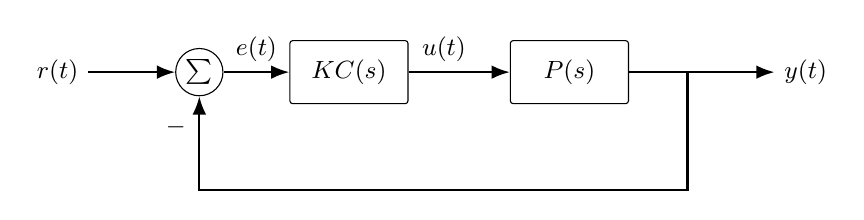
\begin{tikzpicture}[>=Latex,every node/.style={font=\small}]
			\node[align=center] (r) at (-5.5,0) {$r(t)$};
			\node[sumj] (sum) at (-3.7,0) {$\sum$};
			\node[ctlblock] (c) at (-1.8,0) {$K C(s)$};
			\node[ctlblock] (p) at (1,0) {$P(s)$};
			\node[align=center] (y) at (4,0) {$y(t)$};
			\draw[signal] (r) -- (sum);
			\draw[signal] (sum) -- node[above] {$e(t)$} (c);
			\draw[signal] (c) -- node[above,pos=0.35] {$u(t)$} (p);
			\draw[signal] (p) -- (y);
			\draw[signal] (2.5,0) -| (2.5,-1.5) -| (sum.south);
			\node at (-4,-0.7) {$-$};
		\end{tikzpicture}
		\caption{Unity negative-feedback control loop with controller and plant.}
		\label{fig:feedback-loop-basic}
	\end{figure}
	\subsubsection{Mathematical Formulation: Angle and Magnitude Conditions}
	The closed-loop transfer function under unity feedback is: \[
	T(s) = \frac{K G(s)}{1 + K G(s)}
	\] The closed-loop poles are the roots of the characteristic equation: \[
	1 + K G(s) = 0 \iff K G(s) = -1
	\]
	Expressing $-1$ in polar form as a complex number of unit magnitude and odd multiple angle: \[
	-1 = 1 \cdot e^{j(2k+1)\pi}, \quad k \in \{0, \pm 1, \pm 2, \dots\}
	\]
	This yields two conditions:
	\begin{enumerate}
		\item
		\textbf{The Angle Condition (Determines Geometry)}: A point $s_0$ in the complex plane lies on the root locus \textbf{if and only if}: \[
		\angle G(s_0) = \sum_{j=1}^{m} \angle(s_0 - z_j) - \sum_{i=1}^{n} \angle(s_0 - p_i) = \pm 180^\circ(2k + 1)
		\] The net sum of angles from all open-loop zeros minus the angles from all open-loop poles to the test point must equal an odd multiple of $180^\circ$.
		\item
		\textbf{The Magnitude Condition (Determines Gain $K$)}: If a test point $s_0$ satisfies the angle condition, the specific gain $K$ required to place a closed-loop pole at $s_0$ is: \[
		K = \frac{1}{|G(s_0)|} = \frac{\prod_{i=1}^{n} |s_0 - p_i|}{\prod_{j=1}^{m} |s_0 - z_j|} = \frac{\text{Product of pole vector lengths}}{\text{Product of zero vector lengths}}
		\]
	\end{enumerate}
	
	\subsubsection{Systematic Construction Rules for Root Locus ($K \ge 0$)}
	\paragraph{Rule 1: Number of Branches}
	The root locus has $n$ continuous branches, where $n$ is the number of open-loop poles (order of $a(s)$). Each branch tracks the movement of a single closed-loop pole.
	\paragraph{Rule 2: Starting ($K = 0$) and Ending ($K \to \infty$) Points}
	\begin{itemize}
		\item
		As $K \to 0$, the characteristic equation $a(s) + K b(s) = 0$ reduces to $a(s) = 0$. Thus, \textbf{all $n$ branches originate at open-loop poles}.
		\item
		As $K \to \infty$, the equation approaches $b(s) = 0$. Thus, \textbf{$m$ branches terminate at the finite open-loop zeros}.
		\item
		The remaining $n - m$ branches travel toward infinity along straight-line asymptotes to balance the pole excess $n_{pe} = n - m$.
	\end{itemize}
	\paragraph{Rule 3: Symmetry}
	Because complex roots of real polynomials always occur in conjugate pairs, the root locus is \textbf{symmetrical with respect to the real $\sigma$-axis}.
	\paragraph{Rule 4: Real-Axis Segments}
	A point on the real axis lies on the root locus \textbf{if and only if the total number of real open-loop poles and real open-loop zeros to its right is odd}. \textit{(Points to the right of an even number of real poles and zeros produce an angle sum of $k \cdot 360^\circ$, failing the angle condition).}
	\paragraph{Rule 5: Asymptotes for Large Gain ($s \to \infty$)}
	The $n - m$ branches heading to infinity follow straight-line asymptotes radiating from a single real-axis point:
	\begin{itemize}
		\item
		\textbf{Asymptote Centroid ($\sigma_a$)}: \[
		\sigma_a = \frac{\sum_{i=1}^{n} p_i - \sum_{j=1}^{m} z_j}{n - m} = \frac{\sum \text{Poles} - \sum \text{Zeros}}{n - m}
		\]
		\item
		\textbf{Asymptote Angles ($\theta_a$)}: \[
		\theta_a = \frac{(2k + 1)180^\circ}{n - m}, \quad k = 0, 1, 2, \dots, (n - m - 1)
		\]
	\end{itemize}
	\begin{center}\small\begin{tabularx}{\textwidth}{*{4}{Y}}
			\toprule
			\textbf{Pole Excess ($n - m$)} & \textbf{Number of Asymptotes} & \textbf{Asymptote Angles ($\theta_a$)} & \textbf{Geometric Shape} \\
			\midrule
			\textbf{1} & 1 & $180^\circ$ & Single negative real line \\
			\textbf{2} & 2 & $\pm 90^\circ$ & Vertical line parallel to $j\omega$-axis \\
			\textbf{3} & 3 & $60^\circ, 180^\circ, 300^\circ$ (or $\pm 60^\circ, 180^\circ$) & Star radiating toward RHP \\
			\textbf{4} & 4 & $\pm 45^\circ, \pm 135^\circ$ & Crossed axes ($X$-pattern) \\
			\bottomrule
	\end{tabularx}\end{center}
	\paragraph{Rule 6: Breakaway and Break-in Points}
	Where two or more closed-loop poles meet on the real axis and split into the complex plane (breakaway), or where complex branches return to the real axis (break-in):
	\begin{itemize}
		\item
		Along the real axis, gain can be expressed as $K(\sigma) = -\frac{a(\sigma)}{b(\sigma)}$.
		\item
		Breakaway points correspond to local extrema of gain along the real axis, calculated via: \[
		\frac{dK}{ds} = 0 \quad \text{or equivalently} \quad \sum_{j=1}^{m} \frac{1}{\sigma - z_j} = \sum_{i=1}^{n} \frac{1}{\sigma - p_i}
		\]
		\item
		Only solutions $\sigma$ that lie on valid real-axis segments of the root locus represent physical breakaway/break-in coordinates.
	\end{itemize}
	\paragraph{Rule 7: Imaginary Axis ($j\omega$-Axis) Crossings}
	Points where the locus crosses the $j\omega$-axis define the boundary between stability and instability ($K_{\text{crit}}$ and oscillation frequency $\omega_{\text{osc}}$). They are calculated by:
	\begin{enumerate}
		\item
		\textbf{Routh-Hurwitz Stability Criterion}: Construct the Routh array for $\Delta(s) = a(s) + K b(s) = 0$ as a function of $K$. Find the critical gain $K_{\text{crit}}$ that creates a row of zeros (marginal stability), and solve the resulting auxiliary equation for $\pm j\omega_{\text{osc}}$.
		\item
		\textbf{Direct Frequency Substitution}: Substitute $s = j\omega$ into $a(s) + K b(s) = 0$, separate into real and imaginary equations, and solve simultaneously for $K_{\text{crit}}$ and $\omega_{\text{osc}}$.
	\end{enumerate}
	
	\subsubsection{High-Gain Instability Mechanisms}
	The root locus illustrates two common causes of feedback loop destabilization:
	\begin{enumerate}
		\item
		\textbf{High Pole Excess ($n - m \ge 3$)}: When a system has three or more excess poles, the asymptote angles include directions pointing directly into the right-half-plane (e.g., $\theta_a = \pm 60^\circ$ for $n - m = 3$, and $\pm 45^\circ$ for $n - m = 4$). Consequently, as gain $K$ increases, at least two branches must eventually cross the imaginary axis into the RHP. Very high gain will therefore destabilize any plant with $n - m \ge 3$.
		\item
		\textbf{Open-Loop RHP Zeros}: Because every open-loop zero serves as a termination target ($K \to \infty$), any zero in the RHP will pull a closed-loop pole branch across the $j\omega$-axis as gain increases.
	\end{enumerate}
	
	\subsection{Worked Root Locus Example}
	Consider a unity-feedback position control system with open-loop plant: \[
	G(s) = \frac{K}{s(s + 2)(s + 4)}
	\]
	\begin{enumerate}
		\item
		\textbf{Poles and Zeros}: Three poles at $p_1 = 0$, $p_2 = -2$, $p_3 = -4$ ($n = 3$). No finite zeros ($m = 0$). Pole excess $n_{pe} = 3 - 0 = 3$.
		\item
		\textbf{Real-Axis Segments}: Evaluating the number of poles to the right:
		\begin{itemize}
			\item
			Between $0$ and $-2$: 1 pole to the right (odd) $\implies$ \textbf{Locus exists on $[-2, 0]$}.
			\item
			Between $-2$ and $-4$: 2 poles to the right (even) $\implies$ No locus.
			\item
			To the left of $-4$: 3 poles to the right (odd) $\implies$ \textbf{Locus exists on $(-\infty, -4]$}.
		\end{itemize}
		\item
		\textbf{Asymptotes}:
		\begin{itemize}
			\item
			Centroid: $\sigma_a = \frac{0 + (-2) + (-4)}{3} = \frac{-6}{3} = -2.0$.
			\item
			Angles: $\theta_a = \frac{(2k + 1)180^\circ}{3} \in \{60^\circ, 180^\circ, 300^\circ\}$.
		\end{itemize}
		\item
		\textbf{Breakaway Point}: Along the real axis segment between $0$ and $-2$: \[
		K = -s(s + 2)(s + 4) = -(s^3 + 6s^2 + 8s)
		\] \[
		\frac{dK}{ds} = -(3s^2 + 12s + 8) = 0 \implies s = \frac{-12 \pm \sqrt{144 - 96}}{6} = -2 \pm \frac{\sqrt{48}}{6} \approx -2 \pm 1.155
		\]
		\begin{itemize}
			\item
			$s_1 = -0.845$ (lies on $[-2, 0]$ $\implies$ \textbf{Valid breakaway point}).
			\item
			$s_2 = -3.155$ (lies on $[-4, -2]$ $\implies$ Inactive).
		\end{itemize}
		\item
		\textbf{Imaginary Axis Crossing ($j\omega$-Crossing)}: Characteristic equation: $s^3 + 6s^2 + 8s + K = 0$. Forming the Routh array:
		\begin{itemize}
			\item
			$s^3$: $1$, $8$
			\item
			$s^2$: $6$, $K$
			\item
			$s^1$: $\frac{48 - K}{6}$
			\item
			$s^0$: $K$
			Setting the $s^1$ row to zero yields the critical stability gain: \[
			K_{\text{crit}} = 48
			\] The auxiliary equation from the $s^2$ row gives: \[
			6s^2 + 48 = 0 \implies s^2 = -8 \implies s = \pm j\sqrt{8} \approx \pm j 2.83\text{ rad/s}
			\] \textit{Conclusion}: The system is stable for $0 < K < 48$. At $K = 48$, it oscillates continuously at $\omega = 2.83\text{ rad/s}$. For $K > 48$, two poles enter the RHP, causing instability.
		\end{itemize}
	\end{enumerate}
	
	\subsection{Comprehensive Review Matrix}
\begin{center}
	\small
	\begin{tabularx}{\textwidth}{L{0.8} L{0.6} L{1.4}}
		\toprule
		\textbf{Topic / Concept} & \textbf{Mathematical Rule / Formula} & \textbf{Physical \& Design Implications} \\
		\midrule
		\textbf{BIBO Stability} & $\int_0^\infty |g(t)| \, dt < \infty$ & Ensures every bounded input produces a bounded output. \\
		\textbf{Internal Stability} & $\text{Re}(\lambda_i(A)) < 0, \; \forall i$ & Guarantees all state trajectories decay to zero; prevents hidden internal divergence. \\
		\textbf{Pole-Zero Cancellation} & $\Delta(s) = a_p a_c + b_p b_c = 0$ & Cancelling unstable plant poles with controller zeros leaves unstable modes uncontrolled. \\
		\textbf{Dominant Pole Approx.} & $|\text{Re}(p_{\text{non-dominant}})| \ge 5 \cdot |\text{Re}(p_{\text{dominant}})|$ & Non-dominant poles decay rapidly; dynamic response is governed by dominant poles. \\
		\textbf{LHP Zero Effect} & Adds $+ \frac{1}{z}\dot{y}_0(t)$ & Speeds up initial rise time but increases percentage overshoot. \\
		\textbf{RHP Zero Effect} & Adds $- \frac{1}{z}\dot{y}_0(t)$ & Causes non-minimum phase undershoot; limits feedback gain and bandwidth. \\
		\textbf{Root Locus Definition} & $1 + K G(s) = 0, \quad K \in [0, \infty)$ & Maps closed-loop pole locations as feedback gain is adjusted. \\
		\textbf{Angle Condition} & $\angle G(s) = \pm 180^\circ(2k+1)$ & Geometric test to check whether a candidate point lies on the root locus. \\
		\textbf{Magnitude Condition} & $K = \frac{1}{|G(s)|}$ & Determines the exact gain $K$ required to place a closed-loop pole at a valid root locus point. \\
		\textbf{Asymptote Centroid} & $\sigma_a = \frac{\sum p_i - \sum z_j}{n - m}$ & Center of mass from which high-gain asymptotes radiate. \\
		\textbf{Asymptote Angles} & $\theta_a = \frac{(2k+1)180^\circ}{n - m}$ & Radiating directions to infinity; $n - m \ge 3$ branches point toward the RHP. \\
		\textbf{Breakaway Points} & $\frac{dK}{ds} = 0 \iff \sum \frac{1}{\sigma+z_i} = \sum \frac{1}{\sigma+p_i}$ & Transition points where real poles become complex conjugates. \\
		\bottomrule
	\end{tabularx}
\end{center}
	
	\subsection{Interactive Self-Study Questions}
	Test your understanding of Week 3 concepts:
	\begin{enumerate}
		\item
		\textbf{Hidden Instability}: If a plant has a transfer function $P(s) = \frac{s+2}{s-1}$ and you choose a controller $C(s) = \frac{s-1}{s+5}$, the transfer function from command $r$ to output $y$ is $\frac{s+2}{s+5}$ (which has its pole at $-5$). Why will this physical system fail in practice if an external load disturbance acts on the plant input?
		\item
		\textbf{Asymptote Directions}: Without sketching, determine whether a fourth-order plant with one finite zero and unity feedback can be stabilized with arbitrarily large gain $K$.
		\item
		\textbf{Transient Metric Bounds}: If an engineer introduces a lead compensator zero at $s = -1$ to an uncompensated system with dominant poles at $-1 \pm j3$, what changes do you expect in rise time and peak overshoot?
	\end{enumerate}
	
	\newpage
	\section{Improving Transient Response via PD Control}

	\subsection{Master Checklist: Week 4 Core Competencies}
	\begin{itemize}
		\item[$\square$]
		\textbf{Proportional (P) Control Action}: Define the control law $u(t) = K_p e(t)$ and explain how varying $K_p$ influences pole coordinates, system bandwidth, and transient speed.
		\item[$\square$]
		\textbf{P Control on First-Order Plants}: Formulate the closed-loop transfer function and show how gain $K_p$ shortens the time constant $\tau$ and can stabilize open-loop unstable first-order plants.
		\item[$\square$]
		\textbf{Steady-State Offset in Type-0 Systems}: Demonstrate mathematically why pure proportional feedback cannot eliminate steady-state error for step inputs, and formulate the offset as a function of $K_p$.
		\item[$\square$]
		\textbf{Proportional-Derivative (PD) Control Architecture}: Define the ideal PD law $u(t) = K_p e(t) + K_d \frac{de(t)}{dt}$ and its transfer function $C(s) = K_p + K_d s$.
		\item[$\square$]
		\textbf{Predictive Nature of Derivative Action}: Explain why anticipating the rate of change of error provides active damping, counteracting rapid error deviations and suppressing overshoot.
		\item[$\square$]
		\textbf{Second-Order Pole Placement via PD}: Set up the closed-loop characteristic equation with a second-order plant and demonstrate how the two parameters ($K_p, K_d$) permit independent tuning of natural frequency $\omega_n$ and damping ratio $\zeta$.
		\item[$\square$]
		\textbf{Open-Loop Zero Placement}: Show that a PD controller adds a real open-loop zero at $s = -K_p / K_d$, shifting the root locus into the left-half $s$-plane.
		\item[$\square$]
		\textbf{Angle Deficiency Method on the Root Locus}: Compute the angular deficiency $\phi_{\text{def}}$ required to force the root locus through a desired closed-loop pole $s_0$.
		\item[$\square$]
		\textbf{High-Frequency Noise Amplification}: Explain why the unbounded gain of pure differentiation ($|K_d j\omega| \to \infty$) demands practical low-pass derivative filtering.
		\item[$\square$]
		\textbf{Lead Compensator Approximation}: Formulate the transfer function $C(s) = K_c \frac{s + z_c}{s + p_c}$ ($p_c > z_c$) and explain how it approximates PD action while capping high-frequency gain.
		\item[$\square$]
		\textbf{Design Trade-Offs}: Balance the benefits of faster rise time and reduced overshoot against the practical costs of actuator saturation, control effort spikes, and sensor noise transmission.
	\end{itemize}
	
	\subsection{Proportional (P) Control: Dynamics, Pole Motion, and Steady-State Offset}
	\begin{figure}[H]
		\centering
		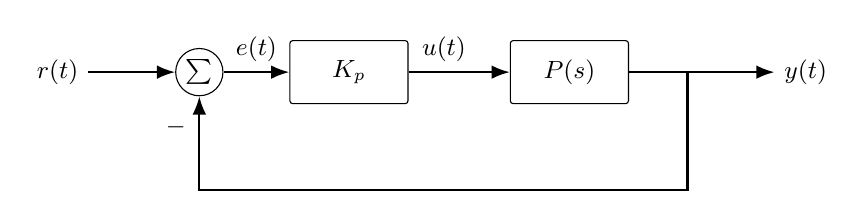
\begin{tikzpicture}[>=Latex,every node/.style={font=\small}]
			\node[align=center] (r) at (-5.5,0) {$r(t)$};
			\node[sumj] (sum) at (-3.7,0) {$\sum$};
			\node[ctlblock] (c) at (-1.8,0) {$K_p$};
			\node[ctlblock] (p) at (1,0) {$P(s)$};
			\node[align=center] (y) at (4,0) {$y(t)$};
			\draw[signal] (r) -- (sum);
			\draw[signal] (sum) -- node[above] {$e(t)$} (c);
			\draw[signal] (c) -- node[above,pos=0.35] {$u(t)$} (p);
			\draw[signal] (p) -- (y);
			\draw[signal] (2.5,0) -| (2.5,-1.5) -| (sum.south);
			\node at (-4,-0.7) {$-$};
		\end{tikzpicture}
		\caption{Proportional control loop with gain $K_p$.}
		\label{fig:p-control-loop}
	\end{figure}
	\subsubsection{Mathematical Definition}
	Proportional control is the simplest feedback mechanism. The control command $u(t)$ is directly proportional to the instantaneous actuating error $e(t) = r(t) - y(t)$: \[
	u(t) = K_p e(t) = K_p [r(t) - y(t)] \quad \Longleftrightarrow \quad C(s) = K_p
	\] The proportional gain $K_p$ acts as an adjustable amplifier that scales the corrective control effort applied to the plant.
	\subsubsection{Action on a Stable First-Order Plant}
	Consider a first-order plant with pole at $s = -a$: \[
	P(s) = \frac{1}{s + a}
	\] Under unity negative feedback, the closed-loop transfer function from reference $r(t)$ to output $y(t)$ is: \[
	G_{ry}(s) = \frac{K_p P(s)}{1 + K_p P(s)} = \frac{K_p}{s + (a + K_p)}
	\]
	\begin{itemize}
		\item
		\textbf{Closed-Loop Pole Location}: The closed-loop pole is located at: \[
		s_{\text{cl}} = -(a + K_p)
		\]
		\item
		\textbf{Time Constant ($\tau$) and Speed}: The closed-loop time constant becomes: \[
		\tau_{\text{cl}} = \frac{1}{a + K_p}
		\] Increasing $K_p > 0$ pushes the closed-loop pole farther to the left along the negative real axis. This accelerates the rate of exponential decay, reducing both the rise time ($T_r \approx 2.2\tau_{\text{cl}}$) and the $2\%$ settling time ($T_s \approx 4\tau_{\text{cl}}$).
		\item
		\textbf{Stabilisation of Unstable Systems}: If the open-loop plant is unstable ($a < 0$, placing the pole in the right-half plane), choosing $K_p > |a|$ shifts the pole into the open left-half plane (OLHP), stabilizing the closed-loop system.
	\end{itemize}
	\subsubsection{The Inevitability of Steady-State Offset in Type-0 Systems}
	Applying a unit step command ($R(s) = 1/s$) to this stable first-order closed-loop system yields the steady-state output via the Final Value Theorem: \[
	y(\infty) = \lim_{s \to 0} s Y(s) = \lim_{s \to 0} s \left( \frac{K_p}{s + a + K_p} \cdot \frac{1}{s} \right) = \frac{K_p}{a + K_p}
	\] The resulting steady-state tracking error is: \[
	e(\infty) = r(\infty) - y(\infty) = 1 - \frac{K_p}{a + K_p} = \frac{a}{a + K_p}
	\]
	\begin{itemize}
		\item
		\textbf{Physical Meaning of Offset}: To hold the output at a nonzero constant value, the physical plant requires a continuous, non-zero driving input $u(\infty)$. Because $u(t) = K_p e(t)$, the error $e(t)$ cannot be zero; if it were, the control input would vanish ($u = 0$), causing the output to decay back to zero.
		\item
		\textbf{Limitation of High Gain}: Although increasing $K_p \to \infty$ reduces $e(\infty)$ towards zero, infinite gain is physically impossible. In higher-order plants ($n \ge 3$), excessive gain pushes root locus branches into the right-half plane, causing oscillations and instability.
	\end{itemize}
	
	\subsection{Proportional-Derivative (PD) Control: Predictive Action \& Dynamic Damping}
	To improve transient speed without causing the excessive oscillations associated with high proportional gains, derivative action is introduced.
	\begin{figure}[H]
		\centering
		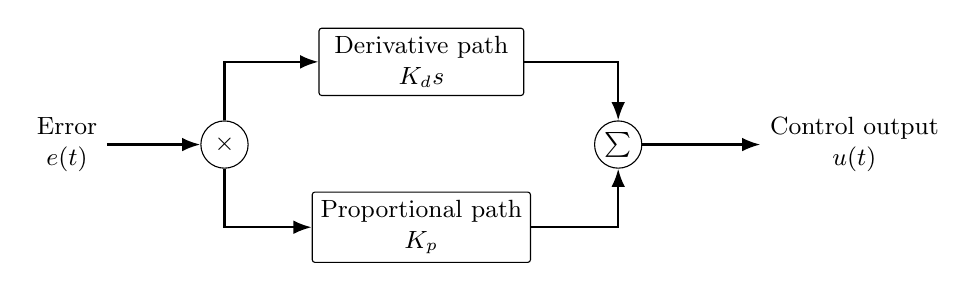
\begin{tikzpicture}[>=Latex,every node/.style={font=\small}]
			\node[align=center] (e) at (-5,0) {Error\\$e(t)$};
			\node[sumj] (split) at (-3,0) {$\times$};
			\node[ctlblock,minimum width=26mm] (d) at (-0.5,1.05) {Derivative path\\$K_d s$};
			\node[ctlblock,minimum width=26mm] (p) at (-0.5,-1.05) {Proportional path\\$K_p$};
			\node[sumj] (sum) at (2,0) {$\sum$};
			\node[align=center] (u) at (5,0) {Control output\\$u(t)$};
			\draw[signal] (e) -- (split);
			\draw[signal] (split) |- (d.west);
			\draw[signal] (split) |- (p.west);
			\draw[signal] (d.east) -| (sum.north);
			\draw[signal] (p.east) -| (sum.south);
			\draw[signal] (sum) -- (u);
		\end{tikzpicture}
		\caption{Parallel proportional and derivative paths in a PD controller. Derivative action responds to the error rate $de(t)/dt$.}
		\label{fig:pd-parallel-structure}
	\end{figure}
	\subsubsection{The Ideal PD Control Law}
	The ideal Proportional-Derivative controller produces a control signal driven by both error magnitude and error velocity: \[
	u(t) = K_p e(t) + K_d \frac{de(t)}{dt} \quad \Longleftrightarrow \quad C(s) = K_p + K_d s = K_d \left( s + \frac{K_p}{K_d} \right)
	\]
	\begin{itemize}
		\item
		\textbf{$K_p$ (Proportional Gain)}: Provides restoring action proportional to the instantaneous displacement from the reference.
		\item
		\textbf{$K_d$ (Derivative Gain)}: Provides viscous damping action proportional to the speed at which the error is changing.
		\item
		\textbf{Open-Loop Zero}: A PD controller introduces an open-loop zero into the forward path at: \[
		s = -z_c = -\frac{K_p}{K_d}
		\]
	\end{itemize}
	\subsubsection{Physical Intuition: Predictive and Anticipatory Action}
	Consider a system approaching its target setpoint rapidly:
	\begin{enumerate}
		\item
		While the instantaneous error $e(t) > 0$ remains positive, the error derivative $\dot{e}(t) < 0$ is negative because the error is shrinking.
		\item
		The derivative term $K_d \dot{e}(t)$ subtracts from the proportional command $K_p e(t)$, applying an early braking action before the output overshoots the setpoint.
		\item
		Conversely, if an external disturbance suddenly deflects the plant away from equilibrium, $\dot{e}(t)$ surges immediately, injecting immediate control effort before a large error accumulates.
	\end{enumerate}
	\subsubsection{Second-Order Pole Placement via PD Control}
	Consider a general uncompensated second-order plant: \[
	P(s) = \frac{K}{s^2 + a_1 s + a_0}
	\] Placing this plant in a unity feedback loop with a PD controller $C(s) = K_p + K_d s$ yields the loop transfer function: \[
	L(s) = P(s)C(s) = \frac{K(K_d s + K_p)}{s^2 + a_1 s + a_0}
	\]
	The closed-loop characteristic equation is: \[
	1 + L(s) = 0 \implies s^2 + a_1 s + a_0 + K(K_d s + K_p) = 0
	\] \[
	\Delta(s) = s^2 + (a_1 + K K_d) s + (a_0 + K K_p) = 0
	\]
	Comparing this with the prototype second-order polynomial $s^2 + 2\zeta\omega_n s + \omega_n^2$ reveals how the parameters are tuned: \[
	\omega_n = \sqrt{a_0 + K K_p}, \qquad 2\zeta\omega_n = a_1 + K K_d \implies \zeta = \frac{a_1 + K K_d}{2\sqrt{a_0 + K K_p}}
	\]
	\begin{center}
		\small
		\begin{tabularx}{\textwidth}{>{\raggedright\arraybackslash}p{0.2\textwidth}Y}
			\toprule
			\textbf{Gain} & \textbf{Primary effect on the closed-loop characteristic polynomial}\\
			\midrule
			Proportional gain $K_p$ & Adjusts the constant coefficient; it is associated with effective stiffness and natural-frequency placement.\\
			Derivative gain $K_d$ & Adjusts the coefficient of the linear-in-$s$ term; it is associated with damping and damping-ratio placement.\\
			\bottomrule
		\end{tabularx}
	\end{center}
	Because $K_p$ and $K_d$ enter separate coefficients, a designer can place the two closed-loop poles at any desired locations in the complex plane. This enables simultaneous tuning of response speed ($\omega_n$) and relative stability ($\zeta$), which is impossible with pure proportional gain.
	
	\subsection{Reshaping the Root Locus via Derivative Compensation}
	When a system's open-loop root locus does not pass through the desired closed-loop pole locations, gain adjustment alone cannot meet the design specifications. Adding a compensator zero pulls the locus toward the left-half plane.

	\subsubsection{The Angle Deficiency Formulation}
	Let $s_0 = -\zeta\omega_n + j\omega_d$ represent the desired closed-loop dominant pole calculated from transient specifications ($T_s, M_p, T_p$). For $s_0$ to lie on the compensated root locus, the loop transfer function must satisfy the Evans Angle Condition: \[
	\angle L(s_0) = \sum_{j=1}^{m} \angle(s_0 - z_j) - \sum_{i=1}^{n} \angle(s_0 - p_i) = \pm 180^\circ(2k + 1)
	\]
	If evaluating the uncompensated plant poles and zeros at $s_0$ yields an angle sum $\theta_{\text{uncomp}} \ne \pm 180^\circ$, the difference is the \textbf{angle deficiency} $\phi_{\text{def}}$: \[
	\phi_{\text{def}} = 180^\circ - \sum_{j=1}^{m} \angle(s_0 - z_j) + \sum_{i=1}^{n} \angle(s_0 - p_i)
	\] The compensator must contribute this angle $\phi_c = \phi_{\text{def}}$ at $s_0$ to pull the locus through the design point.
	\subsubsection{Calculating the Compensator Zero Location}
	For an ideal PD controller $C(s) = K_d(s + z_c)$, the angle contributed by the single zero at $s = -z_c$ is: \[
	\angle(s_0 + z_c) = \theta_z = \phi_{\text{def}}
	\]
	Using the geometry of the complex plane and from trigonometry: \[
	\tan(\theta_z) = \frac{\omega_d}{z_c - \sigma_0} \implies z_c = \sigma_0 + \frac{\omega_d}{\tan(\theta_z)}
	\] where $\sigma_0 = \zeta\omega_n$ and $\omega_d = \omega_n\sqrt{1 - \zeta^2}$. Once the zero is placed, the loop gain $K$ is calculated using the Evans Magnitude Condition: \[
	K = \frac{1}{|P(s_0)C(s_0)|} = \frac{\prod_{i=1}^{n} |s_0 - p_i|}{|s_0 + z_c| \prod_{j=1}^{m} |s_0 - z_j|}
	\]
	
	\subsection{Practical Implementation: Derivative Filtering \& Lead Compensation}
	\subsubsection{The High-Frequency Noise Problem}
	Although ideal PD control ($C(s) = K_p + K_d s$) is mathematically convenient, it \textbf{cannot be implemented with passive physical hardware} because its transfer function is improper ($m > n$). In the frequency domain ($s = j\omega$): \[
	|C(j\omega)| = |K_p + j\omega K_d| = \sqrt{K_p^2 + \omega^2 K_d^2} \xrightarrow{\omega \to \infty} \infty
	\]

	\begin{itemize}
		\item
		\textbf{Amplification of Sensor Noise}: Measurement signals from physical sensors (encoders, tachometers, IMUs) contain high-frequency electronic noise and quantization jitter. Pure differentiation amplifies this high-frequency noise, causing severe actuator chatter, mechanical wear, and driving the amplifier into continuous saturation.
	\end{itemize}
	\subsubsection{Practical Filtered Derivative}
	To resolve this issue, practical controllers add a first-order low-pass filter pole to the derivative term: \[
	C_{\text{filtered}}(s) = K_p + K_d \frac{s}{\frac{s}{N} + 1} = K_p + \frac{K_d N s}{s + N}
	\] where $N$ is the derivative filter coefficient (typically $8 \le N \le 20$).
	\begin{itemize}
		\item
		At low frequencies ($\omega \ll N$), the controller behaves like an ideal differentiator: $\frac{s}{s/N + 1} \approx s$.
		\item
		At high frequencies ($\omega \gg N$), the gain rolls off and is capped at $K_p + K_d N$, preventing noise amplification.
	\end{itemize}
	\subsubsection{Lead Compensator Equivalence}
	Rearranging the filtered PD controller into a rational transfer function reveals its structural equivalence to a \textbf{phase-lead compensator}: \[
	C(s) = \frac{(K_p + K_d N)s + K_p N}{s + N} = K_c \frac{s + z_c}{s + p_c}
	\] where: \[
	z_c = \frac{K_p N}{K_p + K_d N}, \qquad p_c = N, \qquad K_c = K_p + K_d N
	\]
	A \textbf{Lead Compensator} places its pole farther to the left on the real axis than its zero ($p_c > z_c$).
	\begin{itemize}
		\item
		\textbf{Phase Contribution}: Because the zero is closer to the imaginary axis than the pole, its positive phase angle dominates over the pole's negative phase angle, providing a net positive phase lead ($\angle C(j\omega) > 0$) across intermediate frequencies.
		\item
		\textbf{High-Frequency Attenuation}: Unlike pure differentiation, high-frequency gain is strictly bounded by $K_c \frac{p_c}{z_c}$, protecting the physical hardware from sensor noise.
	\end{itemize}
	
	\subsection{Design Trade-Offs and Actuator Constraints}
	Engineering design requires balancing multiple competing performance specifications:
	\begin{center}\small\begin{tabularx}{\textwidth}{*{3}{Y}}
			\toprule
			\textbf{Performance Dimension} & \textbf{Proportional (P) Control} & \textbf{Proportional-Derivative (PD) / Lead Control} \\
			\midrule
			\textbf{Response Speed ($T_r, T_s$)} & High gain reduces rise time and settling time on first-order plants. & Significantly reduces $T_r$ and $T_s$ by shifting dominant poles farther into the OLHP. \\
			\textbf{Damping \& Overshoot ($M_p$)} & High gain degrades relative stability in second- and higher-order plants, increasing overshoot. & The derivative term adds dynamic damping, suppressing overshoot and oscillations. \\
			\textbf{Steady-State Tracking} & Leaves a finite offset error $e_{ss} = \frac{a}{a+K_p}$ on Type-0 plants. & \textbf{Does not eliminate steady-state error}; requires an integrator (PI/PID) to achieve $e_{ss} = 0$. \\
			\textbf{Sensor Noise Sensitivity} & Low sensitivity; proportional gain scales error uniformly across frequencies. & High sensitivity; unmitigated derivative action amplifies high-frequency noise. \\
			\textbf{Actuator Control Effort} & Control effort scales directly with error amplitude: $u(0^+) = K_p \Delta r$. & Produces sharp control effort spikes on step setpoints ($\dot{r} \to \infty$), risking actuator saturation. \\
			\bottomrule
	\end{tabularx}\end{center}
	
	\subsection{Worked Design Example: PD Controller via Root Locus}
	Consider a positioning system with open-loop plant: \[
	P(s) = \frac{10}{s(s + 2)}
	\] \textbf{Design Objective}: Design a controller such that the closed-loop dominant poles have a damping ratio $\zeta = 0.5$ and a settling time $T_s \le 1.0\text{ s}$ ($2\%$ criterion).
	\subsubsection{Step 1: Determine the Desired Closed-Loop Pole Locations}
	From the settling time specification: \[
	\sigma_0 = \zeta\omega_n = \frac{4}{T_s} = \frac{4}{1.0} = 4.0\text{ rad/s}
	\] From the damping ratio $\zeta = 0.5$: \[
	\omega_n = \frac{\sigma_0}{\zeta} = \frac{4.0}{0.5} = 8.0\text{ rad/s}
	\] The damped natural frequency is: \[
	\omega_d = \omega_n \sqrt{1 - \zeta^2} = 8.0 \sqrt{1 - 0.25} = 8.0 \frac{\sqrt{3}}{2} \approx 6.928\text{ rad/s}
	\] Thus, the desired dominant closed-loop pole is: \[
	s_0 = -4.0 + j6.928
	\]
	\subsubsection{Step 2: Evaluate the Uncompensated System at $s_0$}
	Check whether $s_0$ lies on the uncompensated root locus of $P(s) = \frac{10}{s(s + 2)}$:
	\begin{itemize}
		\item
		Angle from pole at $s = 0$: \[
		\theta_{p1} = 180^\circ - \arctan\left(\frac{6.928}{4.0}\right) = 180^\circ - 60.0^\circ = 120.0^\circ
		\]
		\item
		Angle from pole at $s = -2$: \[
		\theta_{p2} = 180^\circ - \arctan\left(\frac{6.928}{4.0 - 2.0}\right) = 180^\circ - \arctan(3.464) = 180^\circ - 73.9^\circ = 106.1^\circ
		\]
		\item
		Sum of uncompensated pole angles: \[
		\sum \theta_p = 120.0^\circ + 106.1^\circ = 226.1^\circ
		\]
	\end{itemize}
	The angle condition requires $180^\circ$. The \textbf{angle deficiency} is: \[
	\phi_{\text{def}} = 226.1^\circ - 180^\circ = 46.1^\circ
	\] Because $\phi_{\text{def}} > 0$, the uncompensated root locus passes to the right of $s_0$, and gain adjustment alone cannot meet the specifications. A PD controller zero must contribute $\theta_z = 46.1^\circ$.
	\subsubsection{Step 3: Calculate the PD Zero Location ($z_c$)}
	From the geometry of the compensator zero: \[
	\tan(46.1^\circ) = \frac{\omega_d}{z_c - \sigma_0} = \frac{6.928}{z_c - 4.0}
	\] \[
	z_c - 4.0 = \frac{6.928}{\tan(46.1^\circ)} = \frac{6.928}{1.039} \approx 6.668 \implies z_c \approx 10.67
	\] The PD controller structure is: \[
	C(s) = K_d(s + 10.67)
	\]
	\subsubsection{Step 4: Calculate the Loop Gain via the Magnitude Condition}
	Evaluate the magnitude condition at $s_0 = -4.0 + j6.928$: \[
	|s_0| = \sqrt{4^2 + 6.928^2} = 8.0
	\] \[
	|s_0 + 2| = \sqrt{(4 - 2)^2 + 6.928^2} = \sqrt{4 + 48} = \sqrt{52} \approx 7.211
	\] \[
	|s_0 + z_c| = |s_0 + 10.67| = \sqrt{(10.67 - 4)^2 + 6.928^2} = \sqrt{6.67^2 + 48} = \sqrt{44.49 + 48} \approx 9.617
	\]
	The loop gain requires: \[
	1 = |C(s_0) P(s_0)| = \frac{10 K_d |s_0 + z_c|}{|s_0| |s_0 + 2|}
	\] \[
	K_d = \frac{|s_0| |s_0 + 2|}{10 |s_0 + z_c|} = \frac{8.0 \times 7.211}{10 \times 9.617} = \frac{57.69}{96.17} \approx 0.60
	\]
	\subsubsection{Step 5: Extract Controller Gains}
	\[
	K_d = 0.60
	\] \[
	K_p = K_d \cdot z_c = 0.60 \times 10.67 \approx 6.40
	\] The final PD controller is: \[
	C(s) = 6.40 + 0.60 s
	\]
	
	\subsection{Comprehensive Review Matrix}
	\begin{center}\small\begin{tabularx}{\textwidth}{L{0.8} L{0.8} L{1.4}}
			\toprule
			\textbf{Component / Parameter} & \textbf{Transfer Function / Governing Formula} & \textbf{Primary Influence on Loop Performance} \\
			\midrule
			\textbf{Proportional Gain ($K_p$)} & $C(s) = K_p$ & Increases response speed and reduces steady-state offset; excessive values induce oscillations. \\
			\textbf{Derivative Gain ($K_d$)} & $C(s) = K_d s$ & Injects phase lead and active damping; reduces overshoot and settling time. \\
			\textbf{Compensator Zero ($z_c$)} & $s = -z_c = -K_p / K_d$ & Pulls root locus branches leftward into the stable region of the $s$-plane. \\
			\textbf{Angle Deficiency ($\phi_{\text{def}}$)} & $\phi_{\text{def}} = 180^\circ - \sum \theta_z + \sum \theta_p$ & Determines the exact phase lead required from the compensator at design point $s_0$. \\
			\textbf{Derivative Filter ($N$)} & $\frac{s}{\frac{s}{N} + 1}$ ($8 \le N \le 20$) & Caps high-frequency controller gain at $K_p + K_d N$, preventing sensor noise amplification. \\
			\textbf{Lead Compensator} & $K_c \frac{s + z_c}{s + p_c}$ with $p_c > z_c$ & Physical, proper realization of PD action; bounds high-frequency gain while providing phase lead. \\
			\bottomrule
	\end{tabularx}\end{center}
	
	\subsection{Interactive Self-Study Questions}
	Test your understanding of Week 4 concepts:
	\begin{enumerate}
		\item
		\textbf{Steady-State Limitations}: Why does adding a PD controller to a Type-0 plant fail to reduce the steady-state tracking error to zero for a constant step reference input?
		\item
		\textbf{Derivative Noise Amplification}: An engineer notes that a motor shaft vibrates with high-frequency jitter after tuning an ideal PD controller. What causes this, and how does adding a low-pass filter pole fix it?
		\item
		\textbf{Lead vs. PD Geometry}: Why does a lead compensator require its pole to be placed deeper into the left-half plane than its zero ($p_c > z_c$), rather than vice versa?
	\end{enumerate}
	
	\newpage
	\section{Improving Steady-State Response via PID Control}	
	\subsection{Master Checklist: Week 5 Core Competencies}
	\begin{itemize}
		\item[$\square$]
		\textbf{Steady-State Error Formulation}: Formulate the closed-loop tracking error $e(t) = r(t) - y(t)$ and apply the \textbf{Final Value Theorem} to derive $e_{ss} = \lim_{s \to 0} s E(s)$ for unity-feedback loops.
		\item[$\square$]
		\textbf{Standard Test Signals}: Characterise the physical role of unit step (position), unit ramp (velocity), and unit parabolic (acceleration) reference inputs.
		\item[$\square$]
		\textbf{System Type Classification}: Define the system type as the number of pure open-loop integrators (multiplicity of poles at $s = 0$) in the loop transfer function $L(s) = P(s)C(s)$.
		\item[$\square$]
		\textbf{Static Error Constants ($K_p, K_v, K_a$)}: Compute the position constant $K_p$, velocity constant $K_v$, and acceleration constant $K_a$, and map them to steady-state error values.
		\item[$\square$]
		\textbf{Disturbance Rejection via Forward-Path Integrators}: Formulate steady-state error due to input load disturbances and demonstrate why placing an integrator upstream of the disturbance eliminates step disturbance offset.
		\item[$\square$]
		\textbf{Non-Unity Feedback Transformations}: Convert non-unity feedback systems into equivalent unity-feedback models to determine true tracking error and system type.
		\item[$\square$]
		\textbf{Proportional-Integral (PI) Architecture}: Define the control law $u(t) = K_p e(t) + K_i \int e(\tau) d\tau$, identify its pole-zero map, and explain how it increases system type by one.
		\item[$\square$]
		\textbf{PI Transient Penalties \& Root Locus Distortion}: Explain why adding an open-loop pole at $s = 0$ increases system order, adds phase lag, and can induce slow transient modes (pole-zero dipoles).
		\item[$\square$]
		\textbf{Passive Lag Compensation}: Formulate $C_{\text{lag}}(s) = K_c \frac{s + z_c}{s + p_c}$ ($z_c > p_c$) and explain how placing a pole-zero pair very close to the origin boosts the static error constant by $z_c / p_c$ without destabilising transient root locus branches.
		\item[$\square$]
		\textbf{Proportional-Integral-Derivative (PID) Control}: Formulate the ideal PID controller with two zeros and one pole at the origin, demonstrating how it simultaneously improves transient damping and eliminates steady-state error.
		\item[$\square$]
		\textbf{PID Algebraic Pole Placement}: Design PID gains ($K_p, K_i, K_d$) to place all closed-loop poles at prescribed locations for a second-order plant.
	\end{itemize}
	
	\subsection{Steady-State Error Formulation \& The Final Value Theorem}
	\begin{figure}[H]
		\centering
		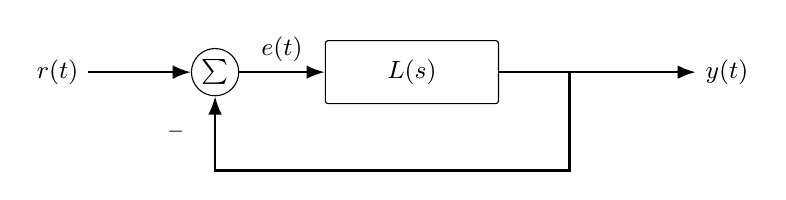
\begin{tikzpicture}[>=Latex,every node/.style={font=\small}]
			\node[align=center] (r) at (-4.5,0) {$r(t)$};
			\node[sumj] (sum) at (-2.5,0) {$\sum$};
			\node[ctlwide] (l) at (0,0) {$L(s)$};
			\node[align=center] (y) at (4,0) {$y(t)$};
			\draw[signal] (r) -- (sum);
			\draw[signal] (sum) -- node[above] {$e(t)$} (l);
			\draw[signal] (l) -- (y);
			\draw[signal] (l) -- ++(2,0) -- ++(0,-1.25) -| (sum.south);
			\node[font=\scriptsize] at (-3,-0.75) {$-$};
		\end{tikzpicture}
		\caption{Unity-feedback loop used to define steady-state error.}
		\label{fig:steady-state-error-loop}
	\end{figure}
	\subsubsection{The Definition of Steady-State Error}
	Steady-state error $e_{ss}$ is the discrepancy between the commanded reference input $r(t)$ and the actual plant output $y(t)$ after all transient natural modes have died out: \[
	e_{ss} \equiv \lim_{t \to \infty} e(t) = \lim_{t \to \infty} [r(t) - y(t)]
	\]
	In the Laplace domain, the actuating error for a unity negative-feedback system with loop transfer function $L(s) = P(s)C(s)$ is given by: \[
	E(s) = R(s) - Y(s) = R(s) - L(s)E(s) \implies E(s) = \frac{1}{1 + L(s)} R(s)
	\]
	\subsubsection{Evaluation via the Final Value Theorem}
	The \textbf{Final Value Theorem (FVT)} enables the calculation of steady-state performance directly from the Laplace domain without computing inverse Laplace transforms: \[
	e_{ss} = \lim_{t \to \infty} e(t) = \lim_{s \to 0} s E(s) = \lim_{s \to 0} \frac{s R(s)}{1 + L(s)}
	\]
	\textbf{Strict Applicability Constraint}: The Final Value Theorem is valid \textbf{if and only if all poles of $s E(s)$ reside strictly in the open left-half of the complex plane (OLHP)}. If the closed-loop system is unstable, or if $s E(s)$ has poles on the imaginary axis or in the right-half plane, the time-domain signal $e(t)$ does not converge to a constant value.
	
	\subsection{System Type and Static Error Constants}
	Steady-state performance depends on the interaction between two characteristics:
	\begin{enumerate}
		\item
		\textbf{The mathematical form of the test input} $R(s)$.
		\item
		\textbf{The number of pure open-loop integrators} contained in the forward loop $L(s)$.
	\end{enumerate}
	\subsubsection{Standard Reference Test Inputs}
	To quantify tracking capabilities, systems are tested against three polynomial test waveforms:
	\begin{enumerate}
		\item
		\textbf{Unit Step Input (Position Command)}: \[
		r(t) = 1(t) \iff R(s) = \frac{1}{s}
		\] Represents an instantaneous setpoint change to a fixed target.
		\item
		\textbf{Unit Ramp Input (Velocity Command)}: \[
		r(t) = t \cdot 1(t) \iff R(s) = \frac{1}{s^2}
		\] Represents a target moving with constant velocity.
		\item
		\textbf{Unit Parabolic Input (Acceleration Command)}: \[
		r(t) = \frac{1}{2}t^2 \cdot 1(t) \iff R(s) = \frac{1}{s^3}
		\] Represents a target moving with constant acceleration.
	\end{enumerate}
	\subsubsection{System Type Definition}
	Express the open-loop transfer function in factored pole-zero form: \[
	L(s) = P(s)C(s) = \frac{K \prod_{j=1}^{m} (s + z_j)}{s^N \prod_{i=1}^{n-N} (s + p_i)}
	\] where $-z_j$ and $-p_i$ represent non-zero finite zeros and poles.
	\begin{itemize}
		\item
		\textbf{System Type}: The integer exponent $N$ representing the \textbf{multiplicity of pure poles at the origin ($s = 0$)} in $L(s)$.
		\begin{itemize}
			\item
			$N = 0 \implies$ \textbf{Type-0 System} (no integrators in the loop).
			\item
			$N = 1 \implies$ \textbf{Type-1 System} (one pure integrator in the loop).
			\item
			$N = 2 \implies$ \textbf{Type-2 System} (two pure integrators in the loop).
		\end{itemize}
	\end{itemize}
	
	\subsubsection{Static Error Constants}
	By substituting the standard test inputs into the Final Value Theorem, three static figures of merit are defined:
	\paragraph{Position Error Constant ($K_p$)}
	Evaluated for a unit step reference $R(s) = 1/s$: \[
	e_{ss,\text{step}} = \lim_{s \to 0} \frac{s \left(\frac{1}{s}\right)}{1 + L(s)} = \frac{1}{1 + \lim_{s \to 0} L(s)} \equiv \frac{1}{1 + K_p}
	\] \[
	K_p \equiv \lim_{s \to 0} L(s)
	\]
	\paragraph{Velocity Error Constant ($K_v$)}
	Evaluated for a unit ramp reference $R(s) = 1/s^2$: \[
	e_{ss,\text{ramp}} = \lim_{s \to 0} \frac{s \left(\frac{1}{s^2}\right)}{1 + L(s)} = \lim_{s \to 0} \frac{1}{s + sL(s)} = \frac{1}{\lim_{s \to 0} s L(s)} \equiv \frac{1}{K_v}
	\] \[
	K_v \equiv \lim_{s \to 0} s L(s)
	\] \textit{(Note: $e_{ss,\text{ramp}}$ is a positional tracking offset measured in output units, not an error in velocity).}
	\paragraph{Acceleration Error Constant ($K_a$)}
	Evaluated for a unit parabolic reference $R(s) = 1/s^3$: \[
	e_{ss,\text{parabola}} = \lim_{s \to 0} \frac{s \left(\frac{1}{s^3}\right)}{1 + L(s)} = \lim_{s \to 0} \frac{1}{s^2 + s^2L(s)} = \frac{1}{\lim_{s \to 0} s^2 L(s)} \equiv \frac{1}{K_a}
	\] \[
	K_a \equiv \lim_{s \to 0} s^2 L(s)
	\]
	
	\subsubsection{Relationships Between System Type, Error Constants, and Steady-State Error}
	Evaluating $K_p, K_v, K_a$ as $s \to 0$ across system types generates the following relationships:
	\begin{center}\small\begin{tabularx}{\textwidth}{*{7}{Y}}
			\toprule
			\textbf{System Type} & \textbf{Position Constant $K_p$} & \textbf{Step Error $e_{ss,\text{step}}$} & \textbf{Velocity Constant $K_v$} & \textbf{Ramp Error $e_{ss,\text{ramp}}$} & \textbf{Acceleration Constant $K_a$} & \textbf{Parabola Error $e_{ss,\text{parabola}}$} \\
			\midrule
			\textbf{Type 0} & Finite Constant $K$ & \textbf{$\frac{1}{1 + K_p}$} & $0$ & \textbf{$\infty$} (diverges) & $0$ & \textbf{$\infty$} (diverges) \\
			\textbf{Type 1} & $\infty$ & \textbf{$0$} (perfect) & Finite Constant $K$ & \textbf{$\frac{1}{K_v}$} & $0$ & \textbf{$\infty$} (diverges) \\
			\textbf{Type 2} & $\infty$ & \textbf{$0$} (perfect) & $\infty$ & \textbf{$0$} (perfect) & Finite Constant $K$ & \textbf{$\frac{1}{K_a}$} \\
			\textbf{Type 3} & $\infty$ & \textbf{$0$} (perfect) & $\infty$ & \textbf{$0$} (perfect) & $\infty$ & \textbf{$0$} (perfect) \\
			\bottomrule
	\end{tabularx}\end{center}
	
	\begin{itemize}
		\item
		\textbf{Finite Errors on the Diagonal}: Finite non-zero steady-state errors appear along the diagonal where input polynomial order matches loop integration order ($N = m$).
		\item
		\textbf{Below the Diagonal ($N > m$)}: Steady-state tracking error is identically zero ($e_{ss} = 0$).
		\item
		\textbf{Above the Diagonal ($N < m$)}: The system cannot track the input; the output lags increasingly behind, and error diverges to infinity.
	\end{itemize}
	
	\subsection{Disturbance Rejection and Non-Unity Feedback}
	\subsubsection{Steady-State Error Caused by Input Load Disturbances}
	Real-world systems are subjected to external load disturbances $D(s)$ (e.g., wind gusts on an antenna, payload changes on a robotic arm, or road slope torque on a vehicle):
	\begin{figure}[H]
		\centering
		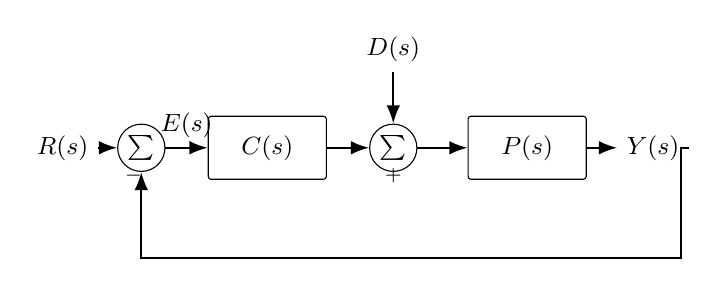
\begin{tikzpicture}[>=Latex,every node/.style={font=\small}]
			\node (r) at (-5,0) {$R(s)$};
			\node[sumj] (s1) at (-4,0) {$\sum$};
			\node[ctlblock] (c) at (-2.4,0) {$C(s)$};
			\node[sumj] (s2) at (-0.8,0) {$\sum$};
			\node[ctlblock] (p) at (0.9,0) {$P(s)$};
			\node (y) at (2.5,0) {$Y(s)$};
			\node (d) at (-0.8,1.25) {$D(s)$};
			\draw[signal] (r) -- (s1);
			\draw[signal] (s1) -- node[above] {$E(s)$} (c);
			\draw[signal] (c) -- (s2);
			\draw[signal] (s2) -- (p);
			\draw[signal] (p) -- (y);
			\draw[signal] (d) -- (s2);
			\draw[signal] (y) -- ++(0.35,0) |- (-3.5,-1.4) -| (s1.south);
			\node[font=\scriptsize] at (-4.1,-0.35) {$-$};
			\node[font=\scriptsize] at (-0.8,-0.35) {$+$};
		\end{tikzpicture}
		\caption{Feedback system with an additive input load disturbance.}
		\label{fig:input-disturbance-loop}
	\end{figure}
	Using superposition, the error transfer function relating reference $R(s)$ and disturbance $D(s)$ to tracking error $E(s) = R(s) - Y(s)$ is: \[
	E(s) = \frac{1}{1 + C(s)P(s)} R(s) - \frac{P(s)}{1 + C(s)P(s)} D(s)
	\]
	Applying the Final Value Theorem for a constant step disturbance $D(s) = \frac{D_0}{s}$ with zero reference ($R(s) = 0$): \[
	e_{D}(\infty) = -\lim_{s \to 0} s \left[ \frac{P(s)}{1 + C(s)P(s)} \cdot \frac{D_0}{s} \right] = -\frac{P(0)}{1 + C(0)P(0)} D_0
	\]
	\begin{itemize}
		\item
		\textbf{Type-0 Control (Finite $C(0) = K_p$)}: A constant disturbance induces a permanent steady-state output offset: $e_D(\infty) = -\frac{P(0)}{1 + K_p P(0)} D_0 \ne 0$.
		\item
		\textbf{Integral Control ($C(s)$ contains $1/s$)}: As $s \to 0$, the controller gain $|C(0)| \to \infty$. Substituting this into the disturbance error equation: \[
		e_{D}(\infty) = -\lim_{s \to 0} \frac{s P(s)}{s + s C(s)P(s)} D_0 = -\frac{P(0)}{\infty} D_0 = 0
		\] An integrator situated in the controller \textbf{completely eliminates steady-state offsets caused by constant step load disturbances}.
	\end{itemize}
	\subsubsection{Non-Unity Feedback Systems}
	When the feedback path contains measurement sensor dynamics $H(s) \ne 1$, the actuating signal $E_a(s) = R(s) - H(s)Y(s)$ is no longer equal to the physical tracking error $E(s) = R(s) - Y(s)$.
	\begin{figure}[H]
		\centering
		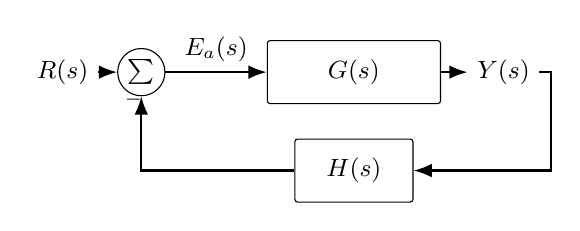
\begin{tikzpicture}[>=Latex,every node/.style={font=\small}]
			\node (r) at (-4.2,0) {$R(s)$};
			\node[sumj] (sum) at (-3.2,0) {$\sum$};
			\node[ctlwide] (g) at (-0.5,0) {$G(s)$};
			\node (y) at (1.4,0) {$Y(s)$};
			\node[ctlblock] (h) at (-0.5,-1.25) {$H(s)$};
			\draw[signal] (r) -- (sum);
			\draw[signal] (sum) -- node[above] {$E_a(s)$} (g);
			\draw[signal] (g) -- (y);
			\draw[signal] (y) -- ++(0.6,0) |- (h.east);
			\draw[signal] (h.west) -| (sum.south);
			\node[font=\scriptsize] at (-3.3,-0.35) {$-$};
		\end{tikzpicture}
		\caption{Non-unity feedback, where the measured output is shaped by $H(s)$.}
		\label{fig:non-unity-feedback}
	\end{figure}
	To compute steady-state error using standard static error constants, convert the loop into an \textbf{algebraically equivalent unity-feedback system}: \[
	T(s) = \frac{G(s)}{1 + G(s)H(s)} \equiv \frac{G_e(s)}{1 + G_e(s)}
	\] Solving for the equivalent forward transfer function $G_e(s)$: \[
	G_e(s) = \frac{G(s)}{1 + G(s)[H(s) - 1]}
	\] Once $G_e(s)$ is established, determine the true system type and evaluate $K_p, K_v, K_a$ as usual.
	
	\subsection{Proportional-Integral (PI) Control: Mechanism \& Dynamics}
	To eliminate steady-state error without requiring impractical infinite proportional gains, an active integrator is placed in the forward loop.
	\begin{figure}[H]
		\centering
		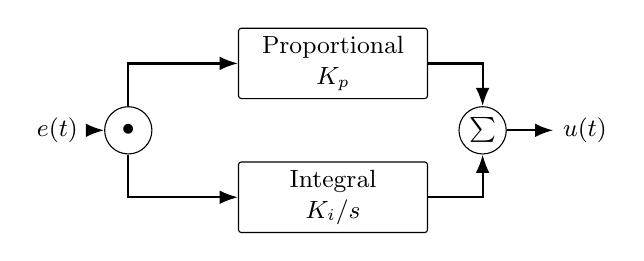
\begin{tikzpicture}[>=Latex,every node/.style={font=\small}]
			\node (e) at (-3.7,0) {$e(t)$};
			\node[sumj] (split) at (-2.8,0) {$\bullet$};
			\node[ctlblock,minimum width=24mm] (p) at (-0.2,0.85) {Proportional\\$K_p$};
			\node[ctlblock,minimum width=24mm] (i) at (-0.2,-0.85) {Integral\\$K_i/s$};
			\node[sumj] (sum) at (1.7,0) {$\sum$};
			\node (u) at (3,0) {$u(t)$};
			\draw[signal] (e) -- (split);
			\draw[signal] (split) |- (p.west);
			\draw[signal] (split) |- (i.west);
			\draw[signal] (p.east) -| (sum.north);
			\draw[signal] (i.east) -| (sum.south);
			\draw[signal] (sum) -- (u);
		\end{tikzpicture}
		\caption{Parallel proportional and integral paths in a PI controller.}
		\label{fig:pi-parallel-structure}
	\end{figure}
	\subsubsection{Mathematical Formulation}
	The continuous-time control law and corresponding transfer function are: \[
	u(t) = K_p e(t) + K_i \int_{0}^{t} e(\tau)\, d\tau \iff C(s) = K_p + \frac{K_i}{s} = \frac{K_p s + K_i}{s}
	\]
	Factoring out the proportional gain: \[
	C(s) = K_p \left( \frac{s + \frac{K_i}{K_p}}{s} \right) = K_p \left( \frac{s + z_i}{s} \right)
	\]
	\begin{itemize}
		\item
		\textbf{Pole at $s = 0$}: Adds an open-loop integrator, increasing the system type by 1 (e.g., converting a Type-0 plant into a Type-1 closed-loop system).
		\item
		\textbf{Zero at $s = -z_i = -K_i / K_p$}: Placed in the left-half plane to balance the destabilising phase lag contributed by the integrator pole.
	\end{itemize}
	\subsubsection{Physical Intuition: The Error Accumulator}
	If a non-zero steady-state tracking error $e_{ss} \ne 0$ were to persist under constant reference and load conditions, the integral term $K_i \int_0^t e(\tau) d\tau$ would integrate a constant over time, ramping $u(t)$ towards $\pm \infty$. Because physical variables in a stable closed-loop cannot grow without bound, the loop can only reach equilibrium when the error is driven to zero: \[
	e_{ss} = 0
	\] The integrator stores the exact steady-state bias voltage/torque required to sustain the output at the setpoint, freeing the proportional error from needing an offset.
	
	\subsubsection{Root Locus Dynamics and Transient Trade-offs}
	While a PI controller eliminates steady-state step error, it alters transient dynamics:
	\begin{lstlisting}
		Effect of PI Controller on the Root Locus
		jomega
		|
		Dominant Pole   |
		x          |
		|          |
		|          |
		-zi             |          |
		-------o--------------x----------x--------------------------> sigma
		PI Zero          ^        Origin
		Extra Closed-   (Pole at 0)
		Loop Pole
	\end{lstlisting}
	\begin{enumerate}
		\item
		\textbf{Increased System Order}: Adding an integrator pole increases the closed-loop system order by one (e.g., a second-order plant becomes a third-order system).
		\item
		\textbf{Phase Lag \& Reduced Stability Margins}: The pole at $s = 0$ contributes $-90^\circ$ of phase lag across low frequencies, pushing the root locus rightward toward the imaginary axis and increasing transient overshoot.
		\item
		\textbf{Pole-Zero Dipole \& Slow Settling Tails}: To preserve the transient response shaped during earlier design stages, the PI zero $z_i$ is placed \textbf{very close to the origin} (e.g., $z_i \in [0.01, 0.1]$).
		\begin{itemize}
			\item
			This forms a \textbf{pole-zero dipole} near $s = 0$.
			\item
			The pole at $0$ and zero at $-z_i$ contribute nearly equal and opposite angles to the dominant high-frequency poles, leaving their location virtually unaltered.
			\item
			\textit{Trade-off}: A closed-loop pole is trapped along the real axis between $0$ and $-z_i$. Although its residue is small due to near cancellation by the zero, it decays slowly with time constant $\tau = 1/z_i$, causing a long "tail" in the step response that lengthens the $2\%$ settling time.
		\end{itemize}
	\end{enumerate}
	
	\subsection{Passive Lag Compensation: Practical Approximation to PI Control}
	\subsubsection{Motivation for Lag Compensation}
	An ideal PI controller requires active electronics (operational amplifiers with low input bias currents and high-quality capacitors) or digital computing hardware to implement the pure integrator. In cost-sensitive or passive analog applications, a \textbf{Phase-Lag Compensator} provides a passive approximation.
	\subsubsection{Transfer Function \& Geometric Placement}
	A lag compensator places its pole off the origin on the negative real axis, with its zero located to the left of the pole: \[
	C_{\text{lag}}(s) = K_c \frac{s + z_c}{s + p_c} \quad \text{where } z_c > p_c > 0
	\]
	\begin{lstlisting}
		Lag Compensator Pole-Zero Map
		jomega
		|
		Zero -zc       Pole -pc|
		-----------------o--------------x----+--------------------------> sigma
		| 0
		<--------------|
		zc > pc (Phase Lag)
	\end{lstlisting}
	Factoring into time-constant form: \[
	C_{\text{lag}}(s) = \hat{K}_c \frac{T s + 1}{\beta T s + 1} = \frac{K_c}{\beta} \frac{s + \frac{1}{T}}{s + \frac{1}{\beta T}}
	\] where: \[
	\beta = \frac{z_c}{p_c} > 1, \qquad T = \frac{1}{z_c}
	\]
	\subsubsection{Low-Frequency Gain Boost \& Minimal Transient Distortion}
	\begin{enumerate}
		\item
		\textbf{Low-Frequency DC Gain Boost}: Evaluating the compensator gain as $s \to 0$: \[
		C_{\text{lag}}(0) = K_c \frac{z_c}{p_c} = K_c \beta
		\] The lag compensator multiplies the static error constant ($K_p$ or $K_v$) by the factor $\beta = \frac{z_c}{p_c}$, reducing steady-state error by a factor of $\beta$: \[
		K_{v,\text{new}} \approx \beta \cdot K_{v,\text{old}} \implies e_{ss,\text{new}} \approx \frac{e_{ss,\text{old}}}{\beta}
		\]
		\item
		\textbf{Transient Isolation Principle}: By choosing $p_c$ and $z_c$ very close to each other near the origin (e.g., $p_c = 0.005, z_c = 0.05 \implies \beta = 10$), the angle contribution to the dominant closed-loop poles $s_0$ is minimal: \[
		\theta_{\text{lag}} = \angle(s_0 + z_c) - \angle(s_0 + p_c) \approx 0^\circ \quad (\text{typically } < 2^\circ \text{ to } 5^\circ)
		\] Because the phase contribution is negligible, the compensated root locus passes through the existing dominant poles without altering transient response speed or damping.
	\end{enumerate}
	
	\subsection{Proportional-Integral-Derivative (PID) Control: Dual Compensation}
	\subsubsection{The Complete Three-Term PID Controller}
	A PID controller combines derivative action (transient shaping and damping) with integral action (steady-state error elimination): \[
	u(t) = K_p e(t) + K_i \int_{0}^{t} e(\tau)\, d\tau + K_d \frac{de(t)}{dt}
	\] \[
	C(s) = K_p + \frac{K_i}{s} + K_d s = \frac{K_d s^2 + K_p s + K_i}{s}
	\]
	\begin{figure}[H]
		\centering
		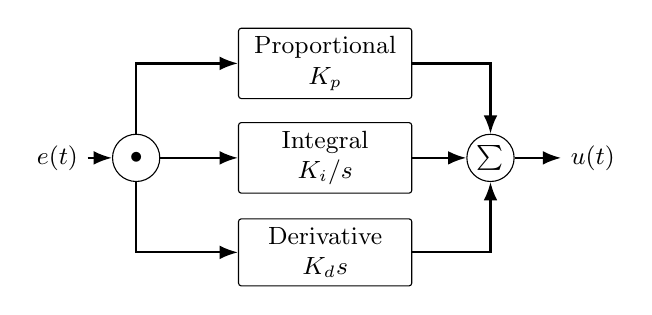
\begin{tikzpicture}[>=Latex,every node/.style={font=\small}]
			\node (e) at (-4,0) {$e(t)$};
			\node[sumj] (split) at (-3,0) {$\bullet$};
			\node[ctlblock,minimum width=22mm] (p) at (-0.6,1.2) {Proportional\\$K_p$};
			\node[ctlblock,minimum width=22mm] (i) at (-0.6,0) {Integral\\$K_i/s$};
			\node[ctlblock,minimum width=22mm] (d) at (-0.6,-1.2) {Derivative\\$K_d s$};
			\node[sumj] (sum) at (1.5,0) {$\sum$};
			\node (u) at (2.8,0) {$u(t)$};
			\draw[signal] (e) -- (split);
			\draw[signal] (split) |- (p.west);
			\draw[signal] (split) -- (i.west);
			\draw[signal] (split) |- (d.west);
			\draw[signal] (p.east) -| (sum.north);
			\draw[signal] (i.east) -- (sum.west);
			\draw[signal] (d.east) -| (sum.south);
			\draw[signal] (sum) -- (u);
		\end{tikzpicture}
		\caption{Three parallel action paths in a PID controller.}
		\label{fig:pid-parallel-structure}
	\end{figure}
	Factoring the numerator quadratic: \[
	C(s) = K_d \frac{(s + z_1)(s + z_2)}{s}
	\]
	\begin{itemize}
		\item
		\textbf{Pole at the origin ($s = 0$)}: Provides integral action to eliminate steady-state error.
		\item
		\textbf{Two Zeros ($-z_1, -z_2$)}:
		\begin{itemize}
			\item
			One zero acts as the \textbf{integral zero}, placed near the origin to preserve low-frequency loop properties.
			\item
			The second zero acts as the \textbf{derivative zero}, placed deeper in the left-half plane to inject phase lead, pull the root locus leftward, and improve transient damping.
		\end{itemize}
	\end{itemize}
	\subsubsection{Arbitrary Second-Order Pole Placement}
	A standard prototype second-order plant possesses two poles. Cascading it with a PID controller produces a third-order closed-loop system with three characteristic coefficients: \[
	P(s) = \frac{1}{s(s + a)} \implies \Delta(s) = s^2(s + a) + (K_d s^2 + K_p s + K_i) = s^3 + (a + K_d)s^2 + K_p s + K_i = 0
	\]
	Because the three controller gains ($K_p, K_i, K_d$) map independently to the three characteristic polynomial coefficients, \textbf{all three closed-loop poles can be assigned arbitrarily}. Designers can place two dominant complex poles for target transient performance ($\zeta, \omega_n$) and place the third real pole far into the OLHP to make it negligible.
	
	\subsection{Worked Design Example: PID Controller via Matched Pole Placement}
	Consider the position control of an inertia-damper system governed by: \[
	P(s) = \frac{1}{s(s + 2)}
	\] \textbf{Design Specifications}:
	\begin{enumerate}
		\item
		\textbf{Steady-State Accuracy}: Zero steady-state error for a unit step input ($e_{ss} = 0$).
		\item
		\textbf{Dominant Transient Dynamics}: Damping ratio $\zeta \approx 0.707$ and natural frequency $\omega_n = \sqrt{2} \approx 1.414\text{ rad/s}$, corresponding to a dominant complex pole pair at: \[
		s_{1,2} = -1 \pm j1
		\]
		\item
		\textbf{Non-Dominant Pole Separation}: The third closed-loop pole must be placed at $s_3 = -4$ (four times farther from the imaginary axis than the dominant real part).
	\end{enumerate}
	\subsubsection{Step 1: Formulate the Target Characteristic Polynomial}
	The desired closed-loop characteristic equation is formed by expanding the three target pole factors: \[
	\Delta_{\text{desired}}(s) = (s - s_3)(s - s_1)(s - s_2) = (s + 4)\left( (s + 1)^2 + 1^2 \right)
	\] \[
	\Delta_{\text{desired}}(s) = (s + 4)(s^2 + 2s + 2) = s^3 + 2s^2 + 2s + 4s^2 + 8s + 8
	\] \[
	\Delta_{\text{desired}}(s) = s^3 + 6s^2 + 10s + 8
	\]
	\subsubsection{Step 2: Formulate the Closed-Loop Characteristic Polynomial with PID}
	Using a standard PID controller $C(s) = K_p + \frac{K_i}{s} + K_d s = \frac{K_d s^2 + K_p s + K_i}{s}$: \[
	L(s) = P(s)C(s) = \frac{K_d s^2 + K_p s + K_i}{s^2(s + 2)}
	\] The closed-loop characteristic equation is $1 + L(s) = 0$: \[
	s^2(s + 2) + (K_d s^2 + K_p s + K_i) = 0
	\] \[
	\Delta(s) = s^3 + (2 + K_d)s^2 + K_p s + K_i = 0
	\]
	\subsubsection{Step 3: Match Coefficients to Solve for Controller Gains}
	Equating corresponding powers of $s$ between $\Delta(s)$ and $\Delta_{\text{desired}}(s)$:
	\begin{enumerate}
		\item
		\textbf{For $s^2$}: \[
		2 + K_d = 6 \implies \mathbf{K_d = 4}
		\]
		\item
		\textbf{For $s^1$}: \[
		K_p = 10 \implies \mathbf{K_p = 10}
		\]
		\item
		\textbf{For $s^0$}: \[
		K_i = 8 \implies \mathbf{K_i = 8}
		\]
	\end{enumerate}
	The designed PID controller transfer function is: \[
	C(s) = 10 + \frac{8}{s} + 4s = \frac{4s^2 + 10s + 8}{s}
	\]
	\subsubsection{Step 4: Verify Steady-State Performance}
	\begin{itemize}
		\item
		The open-loop loop transfer function is: \[
		L(s) = \frac{4s^2 + 10s + 8}{s^2(s + 2)}
		\]
		\item
		Because $L(s)$ contains a factor of $s^2$ in its denominator, the loop is a \textbf{Type-2 system}.
		\item
		For a unit step input: $e_{ss,\text{step}} = 0$.
		\item
		For a unit ramp input: $K_v = \lim_{s \to 0} s L(s) = \infty \implies e_{ss,\text{ramp}} = 0$.
		\item
		For a unit parabolic input: \[
		K_a = \lim_{s \to 0} s^2 L(s) = \lim_{s \to 0} \frac{4s^2 + 10s + 8}{s + 2} = \frac{8}{2} = 4
		\] \[
		e_{ss,\text{parabola}} = \frac{1}{K_a} = \frac{1}{4} = 0.25
		\]
	\end{itemize}
	
	\subsection{Comprehensive Review Matrix}
	\begin{center}\small\begin{tabularx}{\textwidth}{*{6}{Y}}
			\toprule
			\textbf{Controller / Compensator} & \textbf{Transfer Function $C(s)$} & \textbf{System Type Impact} & \textbf{Influence on Static Constants} & \textbf{Primary Effect on Transient Response} & \textbf{Practical Hardware Realization} \\
			\midrule
			\textbf{Proportional (P)} & $K_p$ & Unchanged (Type 0 remains 0) & Increases $K_p$ or $K_v$; cannot make them $\infty$ & Accelerates rise time; degrades damping in high orders & Passive potentiometer or op-amp amplifier \\
			\textbf{Proportional-Derivative (PD)} & $K_p + K_d s$ & Unchanged & Indirectly improves constants by permitting higher $K_p$ & Injects phase lead, suppresses overshoot, shortens settling time & Active op-amp or Lead compensator with filter pole \\
			\textbf{Proportional-Integral (PI)} & $K_p + \frac{K_i}{s}$ & \textbf{Increases by +1} (Type $N \to N+1$) & Drives $K_p \to \infty$, making step tracking error $e_{ss} = 0$ & Adds phase lag; creates slow settling dipole tail near origin & Active analog integrator or embedded digital controller \\
			\textbf{Phase-Lag Compensator} & $K_c \frac{s + z_c}{s + p_c}$ ($z_c > p_c$) & Unchanged (Poles remain off origin) & \textbf{Boosts constants by $\beta = \frac{z_c}{p_c}$} & Preserves transient root locus if dipole is placed close to $0$ & Passive RC ladder network (no external power needed) \\
			\textbf{Proportional-Integral-Derivative (PID)} & $K_p + \frac{K_i}{s} + K_d s$ & \textbf{Increases by +1} (Integrator at $s = 0$) & Eliminates step error and step disturbance offsets & Combines derivative damping with integral steady-state correction & Active op-amp circuit, digital DSP, or passive Lag-Lead \\
			\bottomrule
	\end{tabularx}\end{center}
	
	\subsection{Interactive Self-Study Questions}
	Test your understanding of Week 5 concepts:
	\begin{enumerate}
		\item
		\textbf{System Type \& Constant Errors}: A unity-feedback system with forward loop $L(s) = \frac{20(s+2)}{s(s+5)(s+10)}$ is excited by a ramp input $r(t) = 3t \cdot 1(t)$. What is its system type, static velocity error constant $K_v$, and steady-state tracking error $e_{ss}$?
		\item
		\textbf{Lag vs. PI Selection}: When would a control systems engineer deliberately choose a passive lag compensator over an ideal active PI controller, even though the lag compensator cannot drive steady-state error completely to zero?
		\item
		\textbf{Integral Windup Mechanism}: In physical implementations, an actuator has fixed mechanical or electrical limits (e.g., maximum valve opening or motor supply voltage). If a large setpoint step is applied to a PI controller, what happens to the integral state, and why does this cause severe overshoot when returning to nominal range?
	\end{enumerate}
	
	\newpage
	\section{Practical Aspects of PID Control}

	
	\subsection{Master Checklist: Week 6 Core Competencies}
	\begin{itemize}
		\item[$\square$]
		\textbf{Actuator Saturation \& Integrator Windup}: Explain how physical actuator boundaries ($u_{\min}, u_{\max}$) break the linear feedback loop and cause the integral state to accumulate an excessively large value during sustained errors.
		\item[$\square$]
		\textbf{Anti-Windup via Back-Calculation}: Formulate the tracking anti-windup scheme where the saturation error $e_s(t) = u(t) - v(t)$ is fed back into the integrator state equation with gain $k_t$ (or $1/T_{aw}$) to discharge the accumulated error.
		\item[$\square$]
		\textbf{Alternative Anti-Windup Heuristics}: Contrast back-calculation with \textbf{conditional integration} (freezing the integrator when saturated) and \textbf{integrator clamping}.
		\item[$\square$]
		\textbf{The Ideal Derivative Dilemma}: State the two fundamental operational failures of the ideal differentiator $K_d s$: infinite high-frequency gain amplifying sensor noise and improper transfer function behavior resulting in setpoint kick.
		\item[$\square$]
		\textbf{First-Order Low-Pass Derivative Filtering}: Formulate the practical filtered derivative $\frac{K_d s}{1 + sT_f}$ and apply the industrial rule-of-thumb $T_f = \frac{T_d}{N}$ (with $5 \le N \le 20$) to bound high-frequency gain while preserving phase lead.
		\item[$\square$]
		\textbf{Setpoint Kick Phenomenon}: Explain why applying an abrupt step reference input to an unfiltered error differentiator creates an impulsive spike in the control command.
		\item[$\square$]
		\textbf{Two-Degree-of-Freedom (2-DOF) Setpoint Weighting}: Implement proportional weight $\beta$ and derivative weight $\gamma$ to independently shape reference tracking and transient overshoot without altering closed-loop disturbance rejection or stability.
		\item[$\square$]
		\textbf{Digital Emulation Design Workflow}: Outline the standard process of continuous-time design followed by discrete-time transformation and verification.
		\item[$\square$]
		\textbf{Sampling Period Selection}: Apply the empirical guideline requiring at least 6 to 10 samples across the system rise time or dominant closed-loop time constant.
		\item[$\square$]
		\textbf{Discretization Mapping Methods}: Compare \textbf{Forward Euler} ($s \approx \frac{z-1}{T}$), \textbf{Backward Euler} ($s \approx \frac{z-1}{Tz}$), and the \textbf{Bilinear / Tustin Transform} ($s \approx \frac{2}{T}\frac{z-1}{z+1}$) in terms of frequency warping and preservation of stability.
		\item[$\square$]
		\textbf{Difference Equation Execution}: Convert continuous transfer functions $C(s)$ and $C(z)$ into recursive difference equations $u[k]$ suitable for embedded microcontrollers, PLCs, and DSPs.
		\item[$\square$]
		\textbf{Real-Time Implementation Architecture}: Structure an embedded control loop that minimizes computational latency by transmitting actuator updates before updating background state variables.
	\end{itemize}
	
	\subsection{Actuator Saturation and Integrator Windup}
	\subsubsection{The Physical Saturation Mechanism}
	Linear control models assume that the actuator can deliver any commanded control effort $u(t) \in (-\infty, +\infty)$. In physical systems, every actuator has strict physical saturation limits: \[
	u(t) = \text{sat}(v(t)) = \begin{cases} u_{\max}, & \text{if } v(t) > u_{\max} \\ v(t), & \text{if } u_{\min} \le v(t) \le u_{\max} \\ u_{\min}, & \text{if } v(t) < u_{\min} \end{cases}
	\] where $v(t)$ is the unconstrained controller output (the sum of $P + I + D$ terms) and $u(t)$ is the actual signal applied to the plant.
	\begin{figure}[H]
		\centering
		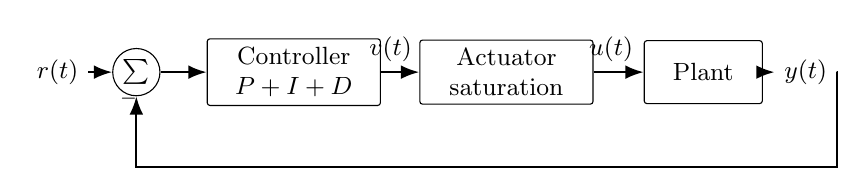
\begin{tikzpicture}[>=Latex,every node/.style={font=\small}]
			\node (r) at (-5,0) {$r(t)$};
			\node[sumj] (sum) at (-4,0) {$\sum$};
			\node[ctlwide] (c) at (-2,0) {Controller\\$P+I+D$};
			\node[ctlwide] (sat) at (0.7,0) {Actuator\\saturation};
			\node[ctlblock] (p) at (3.2,0) {Plant};
			\node (y) at (4.5,0) {$y(t)$};
			\draw[signal] (r) -- (sum);
			\draw[signal] (sum) -- (c);
			\draw[signal] (c) -- node[above,pos=0.25] {$v(t)$} (sat);
			\draw[signal] (sat) -- node[above,pos=0.35] {$u(t)$} (p);
			\draw[signal] (p) -- (y);
			\draw[signal] (y) -- ++(0.4,0) |- (2.2,-1.2) -| (sum.south);
			\node[font=\scriptsize] at (-4.1,-0.34) {$-$};
		\end{tikzpicture}
		\caption{Actuator saturation breaks the expected linear control path between $v(t)$ and $u(t)$.}
		\label{fig:actuator-saturation-loop}
	\end{figure}
	When a large setpoint change or severe external load disturbance occurs, the control output exceeds the actuator's physical limit. Once the actuator saturates at $u_{\max}$ or $u_{\min}$, the feedback loop is effectively broken because the input applied to the plant remains fixed regardless of output variations.
	\subsubsection{The Windup Consequence}
	While the actuator is saturated, the tracking error $e(t) = r(t) - y(t)$ remains non-zero because the actuator cannot deliver enough control authority to drive the plant to the setpoint quickly. Nevertheless, the integral component continues integrating the persistent error: \[
	I(t) = K_i \int_{0}^{t} e(\tau)\, d\tau
	\] The integral state grows to a very large value (it "winds up").
	\begin{lstlisting}
		y(t) ^                                          Commanded Output v(t) (Huge Peak)
		|          Large Settling Overshoot                 ^
		Target|-------------..----------------                    |        . - - - .
		|            /  \                                   |      .'         '.
		|           /    \                               umax|----+-------------+----
		|          /      '-------------                     |    |             |  Actuator
		+---------+---------------------> t                  |    |             |  Saturated
		0         t_cross                                    +----+-------------+-----> t
		0    t_cross       t_unwind
		<------------->
		Lag Period
	\end{lstlisting}
	\begin{itemize}
		\item
		\textbf{Delayed Recovery}: When the plant output $y(t)$ finally crosses the setpoint (at time $t_{\text{cross}}$), the error reverses sign ($e(t) < 0$). However, the accumulated integral state is so large that the unconstrained command $v(t)$ remains far above $u_{\max}$.
		\item
		\textbf{Prolonged Overshoot}: The actuator remains pegged at maximum effort until the negative error has persisted long enough to discharge or "unwind" the accumulated integral state. This produces large transient overshoot, extended settling times, and can induce sustained limit-cycle oscillations.
	\end{itemize}
	
	\subsubsection{Anti-Windup Strategies}
	\paragraph{Strategy 1: Integrator Back-Calculation (Tracking Anti-Windup)}
	Integrator back-calculation dynamically modifies the integrator state equation whenever the actuator saturates.
	\begin{figure}[H]
		\centering
		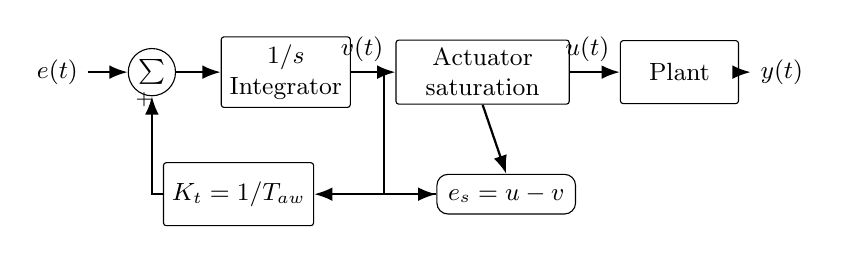
\begin{tikzpicture}[>=Latex,every node/.style={font=\small}]
			\node (e) at (-4.7,0) {$e(t)$};
			\node[sumj] (sum) at (-3.5,0) {$\sum$};
			\node[ctlblock] (int) at (-1.8,0) {$1/s$\\Integrator};
			\node[ctlwide] (sat) at (0.7,0) {Actuator\\saturation};
			\node[ctlblock] (plant) at (3.2,0) {Plant};
			\node (y) at (4.5,0) {$y(t)$};
			\node[draw,rounded corners,align=center,inner sep=4pt] (err) at (1.0,-1.55) {$e_s=u-v$};
			\node[ctlblock] (kt) at (-2.4,-1.55) {$K_t=1/T_{aw}$};
			\draw[signal] (e) -- (sum);
			\draw[signal] (sum) -- (int);
			\draw[signal] (int) -- node[above,pos=0.25] {$v(t)$} (sat);
			\draw[signal] (sat) -- node[above,pos=0.35] {$u(t)$} (plant);
			\draw[signal] (plant) -- (y);
			\draw[signal] (sat.south) -- (err.north);
			\draw[signal] (-0.55,0) -- (-0.55,-1.55) -- (err.west);
			\draw[signal] (err.west) -- (kt.east);
			\draw[signal] (kt.west) -| (sum.south);
			\node[font=\scriptsize] at (-3.6,-0.35) {$+$};
		\end{tikzpicture}
		\caption{Back-calculation anti-windup: the actuator tracking error corrects the integrator state.}
		\label{fig:anti-windup-back-calculation}
	\end{figure}
	\begin{enumerate}
		\item
		\textbf{Saturation Error Calculation}: The saturation error $e_s(t)$ is measured as the difference between the actual saturated actuator output and the unconstrained command: \[
		e_s(t) = u(t) - v(t)
		\]
		\begin{itemize}
			\item
			Under linear operation (no saturation), $u(t) = v(t) \implies e_s(t) = 0$, and the controller operates normally.
			\item
			During positive saturation, $u(t) = u_{\max}$ while $v(t) > u_{\max}$, making $e_s(t) < 0$.
		\end{itemize}
		\item
		\textbf{Modified Integrator Differential Equation}: The saturation error is fed back to the integrator input scaled by an anti-windup tracking gain $k_t = \frac{1}{T_{aw}}$: \[
		\frac{d I_{\text{state}}(t)}{dt} = e(t) + k_t [u(t) - v(t)] = e(t) + \frac{1}{T_{aw}} e_s(t)
		\] where $T_{aw}$ is the anti-windup tracking time constant.
		\item
		\textbf{Dynamic Bleed-off}: When saturation occurs, the negative feedback term $k_t e_s(t)$ actively opposes error accumulation, discharging the integrator state to keep the unconstrained command $v(t)$ close to the saturation boundary. As soon as the error changes sign, the controller immediately comes out of saturation without delay.
		\item
		\textbf{Tuning $k_t$ / $T_{aw}$}: A common design rule is to choose $k_t$ larger than $\frac{K_i}{K_p}$ (or set $T_{aw}$ proportional to the integral time constant $T_i$), providing rapid discharge without amplifying high-frequency measurement noise.
	\end{enumerate}
	\paragraph{Strategy 2: Conditional Integration (Integrator Freezing)}
	Conditional integration stops accumulating error when saturation occurs: \[
	\frac{d I_{\text{state}}(t)}{dt} = \begin{cases} 0, & \text{if } |u(t)| \ge u_{\max} \text{ and } \text{sign}(e(t)) = \text{sign}(u(t)) \\ e(t), & \text{otherwise} \end{cases}
	\] If the actuator is saturated and the current error would drive it deeper into saturation, integration is frozen. Integration resumes only when the error reverses sign or the control command falls back within the linear operating range.
	\paragraph{Strategy 3: Integrator Clamping}
	The integrator state is bounded mathematically between static upper and lower thresholds: \[
	I_{\min} \le I_{\text{state}}(t) \le I_{\max}
	\] This limits total integral windup but does not adapt dynamically to varying load conditions.
	
	\subsection{Derivative Filtering: Eliminating High-Frequency Noise Amplification}
	\subsubsection{The Two Practical Problems of Pure Differentiation}
	The continuous-time ideal derivative term is given by: \[
	u_d(t) = K_d \frac{de(t)}{dt} \iff C_d(s) = K_d s
	\] This ideal representation presents two major implementation problems:
	\begin{enumerate}
		\item
		\textbf{Unbounded High-Frequency Gain}: The transfer function $C_d(s) = K_d s$ is mathematically improper (numerator degree exceeds denominator degree). In the frequency domain ($s = j\omega$): \[
		|C_d(j\omega)| = |K_d j\omega| = K_d \omega \xrightarrow{\omega \to \infty} \infty
		\] High-frequency electronic measurement noise $w(t)$ from sensors enters the controller. Because differentiation scales with frequency $\omega$, high-frequency noise is heavily amplified. This produces large variations in the control command $u(t)$, causing actuator chatter, mechanical wear, and premature saturation.
		\item
		\textbf{Improper Impulse Response (Setpoint Kick)}: An instantaneous step change in reference $r(t)$ produces a discontinuity in tracking error $e(t)$. Differentiating a step discontinuity yields a Dirac delta impulse ($\delta(t)$), demanding an infinite control spike that drives the actuator into immediate saturation.
	\end{enumerate}
	\begin{lstlisting}
		Magnitude |Cd(jomega)| ^
		|                         / Pure Unfiltered Derivative (Slope: +20 dB/dec)
		|                        /
		|                       /
		Kd*N -+----------------------+---------------- Practical Filtered Derivative
		|                     /                  Rolls off to constant gain Kd*N
		|                    /
		|                   /
		1.0 +------------------+
		|                  |
		+------------------+-------------------> Frequency omega (log scale)
		omega_cutoff = 1/Tf = N/Td
	\end{lstlisting}
	
	\subsubsection{First-Order Low-Pass Derivative Filter Formulation}
	To make the differentiator physically realizable and attenuate high-frequency noise, a first-order low-pass filter pole is cascaded with the derivative term: \[
	C_d(s) = \frac{K_d s}{1 + s T_f} = \frac{K_d s}{1 + s \frac{T_d}{N}} = \frac{K_d N s}{s + N/T_d}
	\] where:
	\begin{itemize}
		\item
		$T_d = \frac{K_d}{K_p}$ is the derivative time constant.
		\item
		$T_f$ is the filter time constant.
		\item
		$N$ is the derivative filter factor.
	\end{itemize}
	\paragraph{High-Frequency and Low-Frequency Limits}
	\begin{itemize}
		\item
		\textbf{Low Frequencies ($\omega \ll \frac{1}{T_f}$)}: \[
		1 + j\omega T_f \approx 1 \implies C_d(j\omega) \approx K_d j\omega
		\] The controller acts as an ideal differentiator, providing predictive phase lead and damping transients.
		\item
		\textbf{High Frequencies ($\omega \gg \frac{1}{T_f}$)}: \[
		C_d(j\omega) \approx \frac{K_d j\omega}{j\omega T_f} = \frac{K_d}{T_f} = K_d \frac{N}{T_d} = K_p N
		\] The gain is capped at $K_p N$, providing high-frequency roll-off that limits noise transmission to the actuator.
	\end{itemize}
	\paragraph{Practical Tuning Guidelines for $N$}
	\begin{itemize}
		\item
		In industrial practice, \textbf{$N$ is typically chosen between 5 and 20} (with $N = 10$ serving as a common starting point).
		\item
		Setting $N = 10$ places the filter pole ten times higher in frequency than the zero introduced by the derivative term. This attenuates sensor noise while preserving phase lead near the gain crossover frequency.
		\item
		Choosing $N$ too small (e.g., $N < 2$) introduces phase lag at lower frequencies, reducing the damping benefit of derivative action. Conversely, setting $N$ too large (e.g., $N > 50$) allows excessive high-frequency noise to reach the actuator.
	\end{itemize}
	
	\subsection{Setpoint Weighting \& Two-Degree-of-Freedom (2-DOF) Control}
	\subsubsection{The Setpoint Kick Problem}
	In standard unity-feedback architectures, all three control terms operate on the error signal $e(t) = r(t) - y(t)$: \[
	u(t) = K_p [r(t) - y(t)] + K_i \int [r(\tau) - y(\tau)]\, d\tau + K_d \left[ \frac{dr(t)}{dt} - \frac{dy(t)}{dt} \right]
	\] While external load disturbances $v(t)$ enter smoothly through physical plant dynamics, setpoint changes $r(t)$ are often abrupt steps commanded by operators.
	\begin{itemize}
		\item
		The derivative term acts on $\frac{dr}{dt}$, generating an impulsive spike in the control signal.
		\item
		The proportional term immediately jumps by $K_p \Delta r$, which can cause large overshoot in underdamped systems.
	\end{itemize}
	
	\subsubsection{Two-Degree-of-Freedom PID Architecture}
	To mitigate setpoint kick, the reference signal is weighted using two parameters, $\beta$ and $\gamma$: \[
	u(t) = K_p [\beta r(t) - y(t)] + K_i \int_{0}^{t} [r(\tau) - y(\tau)]\, d\tau + K_d \left[ \gamma \frac{dr(t)}{dt} - \frac{dy(t)}{dt} \right]
	\] where:
	\begin{itemize}
		\item
		$\beta \in [0, 1]$ is the \textbf{proportional setpoint weight}.
		\item
		$\gamma \in [0, 1]$ is the \textbf{derivative setpoint weight}.
	\end{itemize}
	\begin{figure}[H]
		\centering
		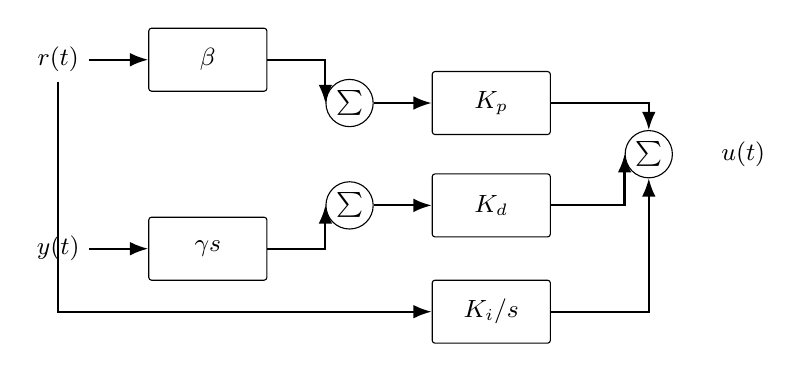
\begin{tikzpicture}[>=Latex,every node/.style={font=\small}]
			\node (r) at (-4.5,1.2) {$r(t)$};
			\node[ctlblock] (beta) at (-2.6,1.2) {$\beta$};
			\node (y) at (-4.5,-1.2) {$y(t)$};
			\node[ctlblock] (gamma) at (-2.6,-1.2) {$\gamma s$};
			\node[sumj] (sum1) at (-0.8,0.65) {$\sum$};
			\node[sumj] (sum2) at (-0.8,-0.65) {$\sum$};
			\node[ctlblock] (p) at (1.0,0.65) {$K_p$};
			\node[ctlblock] (d) at (1.0,-0.65) {$K_d$};
			\node[ctlblock] (i) at (1.0,-2.0) {$K_i/s$};
			\node[sumj] (out) at (3.0,0) {$\sum$};
			\node (u) at (4.2,0) {$u(t)$};
			\draw[signal] (r) -- (beta);
			\draw[signal] (beta.east) -| (sum1.west);
			\draw[signal] (y) -- (gamma);
			\draw[signal] (gamma.east) -| (sum2.west);
			\draw[signal] (sum1) -- (p);
			\draw[signal] (sum2) -- (d);
			\draw[signal] (p.east) -| (out.north);
			\draw[signal] (d.east) -| (out.west);
			\draw[signal] (i.east) -| (out.south);
			\draw[signal] (r) |- (i.west);
		\end{tikzpicture}
		\caption{Two-degree-of-freedom PID architecture with separate reference weighting.}
		\label{fig:two-dof-pid}
	\end{figure}
	\paragraph{Operational Configurations}
	\begin{enumerate}
		\item
		\textbf{Derivative on Measurement Only ($\gamma = 0$)}: Setting $\gamma = 0$ completely removes the reference derivative term: \[
		u_d(t) = -K_d \frac{dy(t)}{dt}
		\] Because the plant output $y(t)$ is physically continuous and cannot jump instantaneously, $\frac{dy}{dt}$ remains finite during step setpoint changes. This eliminates setpoint kick while preserving the dynamic damping needed to attenuate load disturbances.
		\item
		\textbf{Softened Proportional Action ($0 \le \beta < 1$)}: Setting $\beta < 1$ reduces the immediate proportional step response to setpoint changes, lowering peak overshoot. In the extreme case $\beta = 0$, proportional action operates purely on negative output feedback ($-K_p y(t)$), producing a slower, well-damped transition to new setpoints.
		\item
		\textbf{Preservation of Integral Action}: The integral term \textbf{must continue to integrate the unweighted error} $r(t) - y(t)$ to ensure that steady-state tracking error is driven to zero: \[
		e_{ss} = \lim_{t \to \infty} [r(t) - y(t)] = 0
		\] Modifying the integral path would reintroduce steady-state offset.
	\end{enumerate}
	\paragraph{Decoupled Reference Tracking vs. Disturbance Rejection}
	In this 2-DOF formulation, the closed-loop transfer functions for disturbance rejection and reference tracking are decoupled: \[
	Y(s) = G_{yr}(s) R(s) + G_{yv}(s) V(s)
	\] \[
	G_{yv}(s) = \frac{P(s)}{1 + P(s)C(s)}, \qquad G_{yr}(s) = \frac{P(s) C_{\text{ref}}(s)}{1 + P(s)C(s)}
	\]
	\begin{itemize}
		\item
		The denominator $1 + P(s)C(s)$ dictates closed-loop stability, pole locations, and disturbance rejection, which remain unaffected by $\beta$ and $\gamma$.
		\item
		The reference weights $\beta$ and $\gamma$ appear only in the numerator zeros of $G_{yr}(s)$, allowing the transient tracking response to be adjusted without degrading disturbance rejection or stability margins.
	\end{itemize}
	
	\subsection{Discrete-Time Implementation \& Controller Discretization (Emulation Design)}
	Most modern industrial PID controllers are implemented on digital processors (microcontrollers, DSPs, or PLCs) executing discrete algorithms at fixed sampling intervals $T$.
	\begin{figure}[H]
		\centering
		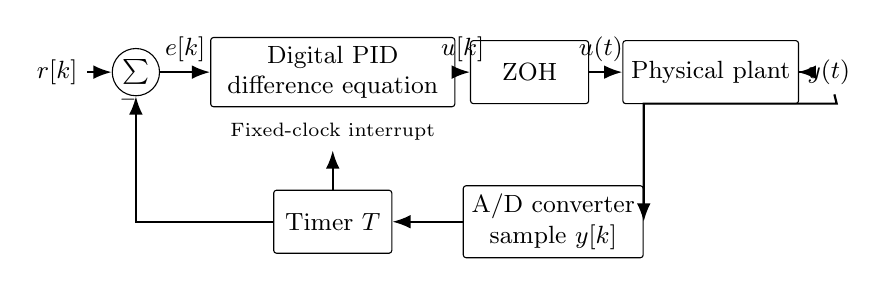
\begin{tikzpicture}[>=Latex,every node/.style={font=\small}]
			\node (r) at (-4.8,0.2) {$r[k]$};
			\node[sumj] (sum) at (-3.8,0.2) {$\sum$};
			\node[ctlwide,minimum width=31mm] (pid) at (-1.3,0.2) {Digital PID\\difference equation};
			\node[ctlblock] (zoh) at (1.2,0.2) {ZOH};
			\node[ctlwide] (plant) at (3.5,0.2) {Physical plant};
			\node (y) at (5.0,0.2) {$y(t)$};
			\node[ctlwide] (adc) at (1.5,-1.7) {A/D converter\\sample $y[k]$};
			\node[ctlblock] (timer) at (-1.3,-1.7) {Timer $T$};
			\draw[signal] (r) -- (sum);
			\draw[signal] (sum) -- node[above] {$e[k]$} (pid);
			\draw[signal] (pid) -- node[above] {$u[k]$} (zoh);
			\draw[signal] (zoh) -- node[above,pos=0.35] {$u(t)$} (plant);
			\draw[signal] (plant) -- (y);
			\draw[signal] (y) -- ++(0.1,-0.4) -| (adc.east);
			\draw[signal] (adc.west) -- (timer.east);
			\draw[signal] (timer.west) -| (sum.south);
			\draw[signal] (timer.north) -- ++(0,0.5) node[above,align=center,font=\scriptsize] {Fixed-clock interrupt};
			\node[font=\scriptsize] at (-3.9,-0.15) {$-$};
		\end{tikzpicture}
		\caption{Sampled-data control loop with digital PID, zero-order hold, plant, and output sampling.}
		\label{fig:digital-control-loop}
	\end{figure}
	\subsubsection{The Emulation Design Methodology}
	\begin{enumerate}
		\item
		\textbf{Continuous Design}: Synthesize and tune the continuous-time controller $C(s)$ to satisfy transient and steady-state requirements.
		\item
		\textbf{Select Sampling Interval $T$}: Choose a sampling rate fast enough to minimize discretization errors and phase delay.
		\item
		\textbf{Discretize}: Map $C(s)$ to an equivalent pulse transfer function $C(z)$ using an algebraic numerical approximation.
		\item
		\textbf{Derive Difference Equation}: Convert $C(z)$ into a causal, recursive difference equation relating current output $u[k]$ to past outputs and error samples.
		\item
		\textbf{Verify via Simulation}: Test the closed-loop discrete system to ensure that sampling delays have not degraded stability margins.
	\end{enumerate}
	
	\subsubsection{Selection of Sampling Period ($T$)}
	\begin{itemize}
		\item
		\textbf{Rise-Time Rule-of-Thumb}: The sampling period $T$ should be chosen to obtain \textbf{at least 6 to 10 samples across the system rise time $T_r$} (or dominant time constant $\tau$): \[
		T \le \frac{T_r}{10} \quad \text{to} \quad \frac{T_r}{6}
		\]
		\item
		\textbf{Bandwidth Rule-of-Thumb}: The sampling frequency $\omega_s = \frac{2\pi}{T}$ should be at least \textbf{10 to 20 times the closed-loop gain crossover bandwidth $\omega_b$}: \[
		\omega_s \ge 10\,\omega_b \implies T \le \frac{2\pi}{10\,\omega_b}
		\]
		\item
		\textbf{The Sampling Trade-off}:
		\begin{itemize}
			\item
			\textit{Sampling too slowly (large $T$)}: Introduces phase lag (approximated by an effective transport delay $T_d \approx T/2$ from zero-order hold reconstruction), which reduces phase margin and can cause instability.
			\item
			\textit{Sampling too quickly (very small $T$)}: Increases computational burden, requires high-precision floating-point arithmetic to avoid numerical rounding issues, and amplifies high-frequency sensor noise.
		\end{itemize}
	\end{itemize}
	
	\subsubsection{Continuous-to-Discrete Approximation Methods}
	\paragraph{Method 1: Forward Euler (Forward Difference)}
	Approximates the continuous derivative via a forward difference: \[
	s \approx \frac{z - 1}{T} \iff \frac{1}{s} \approx \frac{T}{z - 1}
	\]
	\begin{itemize}
		\item
		\textit{Stability Mapping}: Maps the stable continuous left-half $s$-plane into a shifted region $\text{Re}(z) < 1$.
		\item
		\textit{Limitation}: Continuous-time stable poles can map outside the unit circle on the $z$-plane if $T$ is not sufficiently small, making this method prone to instability.
	\end{itemize}
	\paragraph{Method 2: Backward Euler (Backward Difference)}
	Approximates the derivative via a backward difference: \[
	s \approx \frac{z - 1}{T z} = \frac{1 - z^{-1}}{T} \iff \frac{1}{s} \approx \frac{T z}{z - 1} = \frac{T}{1 - z^{-1}}
	\]
	\begin{itemize}
		\item
		\textit{Stability Mapping}: Maps the entire continuous left-half $s$-plane inside a circle of radius $0.5$ centered at $z = 0.5$ within the unit circle.
		\item
		\textit{Properties}: Inherently stable; every stable continuous-time pole maps to a stable discrete-time pole inside the unit circle.
	\end{itemize}
	\paragraph{Method 3: Bilinear (Tustin) Transform (Trapezoidal Approximation)}
	Approximates integration using the trapezoidal rule: \[
	s \approx \frac{2}{T} \left( \frac{z - 1}{z + 1} \right) \iff \frac{1}{s} \approx \frac{T}{2} \left( \frac{z + 1}{z - 1} \right)
	\]
	\begin{itemize}
		\item
		\textit{Stability Mapping}: \textbf{Maps the entire open left-half $s$-plane directly into the interior of the discrete unit circle} ($|z| < 1$).
		\item
		\textit{Frequency Preservation}: A stable continuous-time controller is guaranteed to produce a stable digital controller.
		\item
		\textit{Industrial Standard}: Recommended for high-performance controller discretization due to its balance of stability preservation and accuracy.
	\end{itemize}
	
	\subsubsection{Worked Discretization Example: PI Controller via Bilinear Transform}
	Consider a continuous PI controller designed for velocity control: \[
	C(s) = 2 + \frac{5}{s} = \frac{2s + 5}{s}
	\] \textbf{Task}: Discretize this controller using the Bilinear (Tustin) transform with a sampling period of $T = 0.1\text{ s}$, and derive the executable difference equation.
	\paragraph{Step 1: Substitute the Tustin Operator}
	Using $T = 0.1\text{ s}$: \[
	s \approx \frac{2}{0.1} \left( \frac{z - 1}{z + 1} \right) = 20 \left( \frac{z - 1}{z + 1} \right)
	\]
	Substitute into $C(s)$: \[
	C(z) = 2 + \frac{5}{20 \left( \frac{z - 1}{z + 1} \right)} = 2 + \frac{5(z + 1)}{20(z - 1)} = 2 + \frac{z + 1}{4(z - 1)}
	\]
	\paragraph{Step 2: Combine and Simplify}
	Express over a common denominator: \[
	C(z) = \frac{8(z - 1) + (z + 1)}{4(z - 1)} = \frac{8z - 8 + z + 1}{4(z - 1)} = \frac{9z - 7}{4(z - 1)} = \frac{2.25z - 1.75}{z - 1}
	\]
	Factoring in terms of negative powers of $z$ (backward delay operators $z^{-1}$): \[
	C(z) = \frac{U(z)}{E(z)} = \frac{2.25 - 1.75 z^{-1}}{1 - z^{-1}}
	\]
	\paragraph{Step 3: Transform to the Discrete-Time Domain}
	Cross-multiply to formulate the algebraic relationship: \[
	U(z) (1 - z^{-1}) = E(z) (2.25 - 1.75 z^{-1})
	\] \[
	U(z) - z^{-1} U(z) = 2.25 E(z) - 1.75 z^{-1} E(z)
	\]
	Taking the inverse $Z$-transform (where $z^{-1} X(z) \iff x[k-1]$): \[
	u[k] - u[k - 1] = 2.25 e[k] - 1.75 e[k - 1]
	\]
	Rearranging into recursive update form: \[
	u[k] = u[k - 1] + 2.25 e[k] - 1.75 e[k - 1]
	\] This recursive difference equation can be executed directly within an embedded interrupt service routine every $0.1\text{ s}$.
	
	\subsection{Practical Software Implementation \& Embedded Architecture}
	When implementing a complete PID controller in software, the algorithm must incorporate \textbf{anti-windup}, \textbf{derivative filtering}, \textbf{setpoint weighting}, and an \textbf{execution sequence that minimizes latency}.
	\begin{figure}[H]
		\centering
		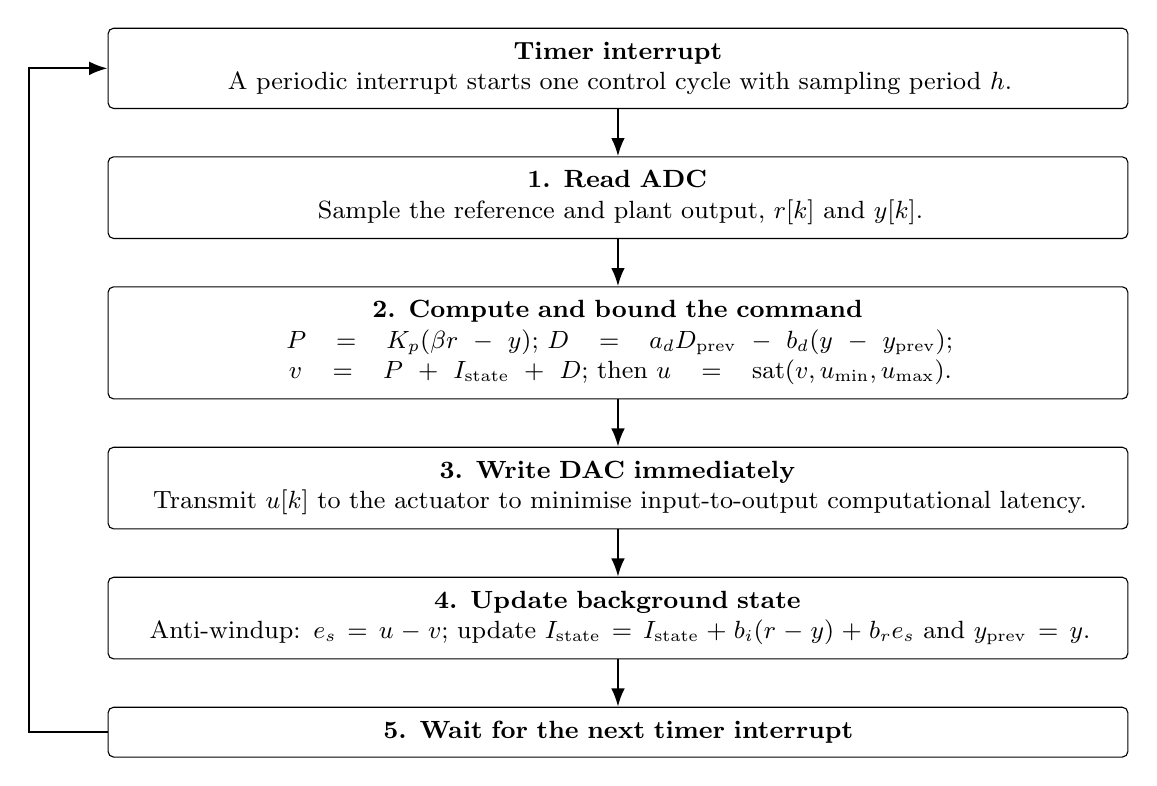
\begin{tikzpicture}[node distance=6mm,>=Latex,every node/.style={font=\small}]
			\node[flowbox] (start) {\textbf{Timer interrupt}\\A periodic interrupt starts one control cycle with sampling period $h$.};
			\node[flowbox,below=of start] (read) {\textbf{1. Read ADC}\\Sample the reference and plant output, $r[k]$ and $y[k]$.};
			\node[flowbox,below=of read] (compute) {\textbf{2. Compute and bound the command}\\$P=K_p(\beta r-y)$; $D=a_dD_{\mathrm{prev}}-b_d(y-y_{\mathrm{prev}})$;\\$v=P+I_{\mathrm{state}}+D$; then $u=\operatorname{sat}(v,u_{\min},u_{\max})$.};
			\node[flowbox,below=of compute] (write) {\textbf{3. Write DAC immediately}\\Transmit $u[k]$ to the actuator to minimise input-to-output computational latency.};
			\node[flowbox,below=of write] (update) {\textbf{4. Update background state}\\Anti-windup: $e_s=u-v$; update $I_{\mathrm{state}}=I_{\mathrm{state}}+b_i(r-y)+b_r e_s$ and $y_{\mathrm{prev}}=y$.};
			\node[flowbox,below=of update] (sleep) {\textbf{5. Wait for the next timer interrupt}};
			\draw[flowarrow] (start) -- (read);
			\draw[flowarrow] (read) -- (compute);
			\draw[flowarrow] (compute) -- (write);
			\draw[flowarrow] (write) -- (update);
			\draw[flowarrow] (update) -- (sleep);
			\draw[flowarrow] (sleep.west) -- ++(-1.0,0) |- (start.west);
		\end{tikzpicture}
		\caption{Real-time execution sequence for a sampled PID controller with actuator limiting and anti-windup.}
		\label{fig:pid-real-time-workflow}
	\end{figure}
	\subsubsection{Precomputed Difference Equations}
	To minimize execution time within the interrupt service routine, constant coefficients are precomputed prior to loop execution:
	\begin{itemize}
		\item
		$b_i = K_i h$ (where $h$ is the sampling interval $T$).
		\item
		$a_d = \frac{T_f}{T_f + h}$ and $b_d = \frac{K_d}{T_f + h}$ (from backward difference on the filtered derivative).
		\item
		$b_r = \frac{h}{T_{aw}}$ (anti-windup reset coefficient).
	\end{itemize}
	\subsubsection{Latency Minimization Architecture}
	A common design flaw in digital control loops is performing all background state updates before writing the output to the digital-to-analog converter (DAC).
	\begin{itemize}
		\item
		\textbf{Best-Practice Sequence}: Read the analog-to-digital converter (ADC), evaluate the minimal algebraic operations needed for $u[k]$, and \textbf{immediately send $u[k]$ to the DAC}.
		\item
		Background tasks—such as updating integral states with anti-windup terms, storing historical values $y_{\text{prev}}$, and logging telemetry—are computed after the actuator signal has been transmitted. This minimizes computational phase lag in the feedback loop.
	\end{itemize}
	
	\subsection{Comprehensive Review Matrix: Practical PID Modifications}
	\begin{center}\small\begin{tabularx}{\textwidth}{*{4}{Y}}
			\toprule
			\textbf{Modification} & \textbf{Primary Failure Mode Addressed} & \textbf{Mathematical Governing Formula} & \textbf{Real-Time Hardware Benefit} \\
			\midrule
			\textbf{Integrator Anti-Windup} & Actuator saturation causing large overshoot and long recovery delays. & $\frac{dI}{dt} = e + k_t [u_{\text{sat}} - v]$ & Prevents integral state accumulation during saturation; enables immediate recovery when error reverses. \\
			\textbf{Derivative Filtering} & Unbounded gain ($K_d \omega$) amplifying sensor noise and causing actuator chatter. & $C_d(s) = \frac{K_d s}{1 + s T_f}$ with $T_f = \frac{T_d}{N}$ ($5 \le N \le 20$) & Caps high-frequency gain at $K_p N$, providing roll-off that protects actuators from noise while retaining phase lead. \\
			\textbf{Derivative on Measurement} & Setpoint kick (impulsive control spikes caused by step changes in reference). & $u_d(t) = -K_d \frac{dy(t)}{dt}$ ($\gamma = 0$) & Smooths control effort during setpoint changes without degrading disturbance rejection. \\
			\textbf{Setpoint Weighting (2-DOF)} & Excessive transient overshoot from step reference inputs. & $u_p(t) = K_p [\beta r(t) - y(t)]$ with $0 \le \beta \le 1$ & Decouples reference tracking from disturbance rejection, allowing overshoot reduction without changing loop poles. \\
			\textbf{Bilinear (Tustin) Discretization} & Instability and frequency distortion during continuous-to-discrete conversion. & $s \approx \frac{2}{T} \left( \frac{z - 1}{z + 1} \right)$ & Maps the entire stable continuous left-half $s$-plane inside the discrete unit circle, preserving stability. \\
			\bottomrule
	\end{tabularx}\end{center}
	
	\subsection{Interactive Self-Study Questions}
	Test your understanding of Week 6 concepts:
	\begin{enumerate}
		\item
		\textbf{Anti-Windup Dynamics}: If the anti-windup tracking gain $k_t$ is set to zero, how does the back-calculation equation behave, and what happens to the closed-loop step response when driving an actuator into saturation?
		\item
		\textbf{Derivative Filter Cutoff}: Why is setting the derivative filter factor $N = 1$ (where $T_f = T_d$) generally considered too aggressive for systems requiring fast transient damping?
		\item
		\textbf{Discrete Stability Limits}: If a continuous plant is controlled by a discrete PID algorithm designed via emulation, why does increasing the sampling interval $T$ eventually drive the closed-loop system toward instability, even when using the Bilinear transform?
	\end{enumerate}
	
	\newpage
	\section{State space models}
	
	\subsection{Foundations of Continuous-Time State-Space Models}
	\subsubsection{Revision Checklist}
	\begin{itemize}
		\item[$\square$]
		\textbf{Define the state vector} $x(t)$ and explain why $n$ first-order ordinary differential equations (ODEs) can represent an $n$-th order physical system.
		\item[$\square$]
		\textbf{Distinguish between dimensions} of inputs ($p$), states ($n$), and outputs ($q$) for SISO and MIMO systems.
		\item[$\square$]
		\textbf{State the general continuous-time state-space equations} in matrix form and define each constituent matrix ($A, B, C, D$).
		\item[$\square$]
		\textbf{Explain the physical meaning of the direct feedthrough matrix} $D$ and identify when $D = 0$.
	\end{itemize}
	
	\subsubsection{Core Concepts \& Formulations}
	\paragraph{State-Space Representation}
	A continuous-time linear state-space model with $p$ inputs, $q$ outputs, and $n$ state variables is expressed as: \[
	\dot{x}(t) = Ax(t) + Bu(t)
	\] \[
	y(t) = Cx(t) + Du(t)
	\]
	\begin{itemize}
		\item
		\textbf{State Vector} $x(t) \in \mathbb{R}^n$: The minimal set of internal dynamic variables that completely summarize the past history of the system, enabling the exact prediction of its future state trajectory given future inputs. The dimension $n$ is the \textbf{order} of the system.
		\item
		\textbf{Input Vector} $u(t) \in \mathbb{R}^p$: The external driving signals or control inputs applied to the system actuators. If $p = 1$, the system is \textbf{single-input}; if $p > 1$, it is \textbf{multi-input}.
		\item
		\textbf{Output Vector} $y(t) \in \mathbb{R}^q$: The measured signals or variables of interest provided by system sensors. If $q = 1$, the system is \textbf{single-output}; if $p = q = 1$, the system is \textbf{single-input single-output (SISO)}; if $p, q > 1$, it is \textbf{multiple-input multiple-output (MIMO)}.
		\item
		\textbf{System (Dynamics) Matrix} $A \in \mathbb{R}^{n \times n}$: Characterizes the internal coupling, autonomous interactions, and natural unforced modes among the state variables.
		\item
		\textbf{Input Matrix} $B \in \mathbb{R}^{n \times p}$: Dictates how external control inputs enter and influence the state derivatives.
		\item
		\textbf{Output Matrix} $C \in \mathbb{R}^{q \times n}$: Maps the internal system states to the measurable output quantities.
		\item
		\textbf{Direct Transmission (Feedthrough) Matrix} $D \in \mathbb{R}^{q \times p}$: Represents an instantaneous, algebraic bypass path directly from the input to the output. In strictly proper physical systems where inputs cannot jump through to outputs with zero delay, $D = 0$.
	\end{itemize}
	
	\subsection{Time-Domain Solutions \& The Matrix Exponential}
	\subsubsection{Revision Checklist}
	\begin{itemize}
		\item[$\square$]
		\textbf{Define the matrix exponential} $\exp(At)$ via its infinite power series and state its derivative property.
		\item[$\square$]
		\textbf{State the linear decomposition principle} separating the complete response into zero-input and zero-state solutions.
		\item[$\square$]
		\textbf{Derive the zero-input response} $x_{\text{zi}}(t)$ and verify initial condition satisfaction.
		\item[$\square$]
		\textbf{Formulate the zero-state response} $x_{\text{zs}}(t)$ as a matrix convolution integral.
		\item[$\square$]
		\textbf{Write down the full solution} for both the state vector $x(t)$ and output vector $y(t)$ for $t \ge 0$.
	\end{itemize}
	
	\subsubsection{Core Concepts \& Formulations}
	\paragraph{The Matrix Exponential}
	For an $n \times n$ matrix $A$, the matrix exponential is defined by the globally convergent power series: \[
	\exp(At) = e^{At} = \sum_{k=0}^{\infty} \frac{t^k}{k!} A^k = I + At + \frac{A^2 t^2}{2!} + \frac{A^3 t^3}{3!} + \dots
	\]
	Differentiating this series term-by-term with respect to time confirms the fundamental identity: \[
	\frac{d}{dt}\exp(At) = \sum_{k=1}^{\infty} \frac{k t^{k-1}}{k!} A^k = A \sum_{\ell=0}^{\infty} \frac{t^\ell}{\ell!} A^\ell = A \exp(At) = \exp(At)A
	\]
	Furthermore, the matrix exponential satisfies the exponential composition law: \[
	\exp((t - \tau)A) = \exp(tA)\exp(-\tau A)
	\] with $\exp(0) = I$.
	\paragraph{Response Decomposition}
	Due to linearity, the overall state solution splits into two decoupled components: \[
	x(t) = x_{\text{zi}}(t) + x_{\text{zs}}(t)
	\]
	\begin{enumerate}
		\item
		\textbf{Zero-Input Response ($x_{\text{zi}}(t)$):} The response driven purely by the initial state $x(0) = x_0$ with no input applied ($u(t) = 0$): \[
		x_{\text{zi}}(t) = \exp(At)x_0, \quad t \ge 0
		\] \textit{Verification:} Evaluating at $t = 0$ yields $x_{\text{zi}}(0) = \exp(0)x_0 = I x_0 = x_0$. Differentiating confirms $\dot{x}_{\text{zi}}(t) = A\exp(At)x_0 = Ax_{\text{zi}}(t)$.
		\item
		\textbf{Zero-State Response ($x_{\text{zs}}(t)$):} The response starting from rest ($x_0 = 0$), driven purely by the input history $u(t)$ via the convolution integral: \[
		x_{\text{zs}}(t) = \int_{0}^{t} \exp(A(t - \tau))Bu(\tau)\, d\tau, \quad t \ge 0
		\] This represents the convolution of the matrix-valued impulse response kernel $\exp(At)B\mathbf{1}(t)$ with the vector-valued control signal $u(t)\mathbf{1}(t)$.
	\end{enumerate}
	\paragraph{Complete Analytical Solution}
	Combining both contributions yields the total time-domain state trajectory and output trajectory: \[
	x(t) = \exp(At)x_0 + \int_{0}^{t} \exp(A(t - \tau))Bu(\tau)\, d\tau
	\] \[
	y(t) = C\exp(At)x_0 + \int_{0}^{t} C\exp(A(t - \tau))Bu(\tau)\, d\tau + Du(t)
	\]
	
	\subsection{Transfer Functions \& Frequency-Domain Realizations}
	\subsubsection{Revision Checklist}
	\begin{itemize}
		\item[$\square$]
		\textbf{Derive the transfer function matrix} $G(s) = C(sI - A)^{-1}B + D$ by taking the Laplace transform of the state-space model.
		\item[$\square$]
		\textbf{Relate the resolvent matrix} $(sI - A)^{-1}$ to the Laplace transform of the matrix exponential $\exp(At)$.
		\item[$\square$]
		\textbf{Express $(sI - A)^{-1}$ using the adjugate and determinant} to analyze system poles.
		\item[$\square$]
		\textbf{Explain the relationship between the eigenvalues of $A$ and the poles of $G(s)$}, including the critical effect of pole-zero cancellations.
	\end{itemize}
	
	\subsubsection{Core Concepts \& Formulations}
	\paragraph{Derivation of the Transfer Function}
	Applying the unilateral Laplace transform to the state-space equations with initial condition $x(0) = x_0$ yields: \[
	sX(s) - x_0 = AX(s) + BU(s) \implies (sI - A)X(s) = x_0 + BU(s)
	\] \[
	X(s) = (sI - A)^{-1}x_0 + (sI - A)^{-1}BU(s)
	\]
	Substituting $X(s)$ into the Laplace transform of the output equation $Y(s) = CX(s) + DU(s)$ gives: \[
	Y(s) = C(sI - A)^{-1}x_0 + \left[ C(sI - A)^{-1}B + D \right] U(s)
	\]
	For zero initial conditions ($x_0 = 0$), the input-output relationship simplifies to the transfer function (or transfer matrix in MIMO systems): \[
	G(s) = \frac{Y(s)}{U(s)} = C(sI - A)^{-1}B + D
	\]
	\paragraph{Laplace Transform of the Matrix Exponential}
	The matrix function $\exp(At)\mathbf{1}(t)$ has the Laplace transform: \[
	\mathcal{L}\{\exp(At)\mathbf{1}(t)\} = \int_{0}^{\infty} \exp(At)e^{-st} \, dt = (sI - A)^{-1}
	\] which directly mirrors the scalar Laplace pair $\mathcal{L}\{e^{at}\mathbf{1}(t)\} = \frac{1}{s - a}$.
	\paragraph{Poles vs. Eigenvalues}
	Using the matrix inverse identity $M^{-1} = \frac{1}{\det(M)} \text{adj}(M)$, the transfer function can be written as: \[
	G(s) = \frac{1}{\det(sI - A)} C \text{adj}(sI - A) B + D = \frac{b(s)}{\det(sI - A)}
	\] where each entry of $\text{adj}(sI - A)$ is a polynomial in $s$ of degree at most $n - 1$.
	\begin{itemize}
		\item
		\textbf{Eigenvalues of $A$:} The scalar roots of the characteristic equation $\det(sI - A) = 0$.
		\item
		\textbf{Poles of $G(s)$:} The singularities where $G(s) \to \infty$.
		\item
		\textbf{Core Rule:} \textbf{Every pole of $G(s)$ is an eigenvalue of $A$}. However, the converse does not always hold: if an internal state is uncoupled from either the input or the output, algebraic pole-zero cancellations occur between $b(s)$ and $\det(sI - A)$. Such cancelled eigenvalues remain internal natural modes of $A$ but disappear from the external transfer function $G(s)$.
	\end{itemize}
	
	\subsection{Coordinate Transformations \& Similarity}
	\subsubsection{Revision Checklist}
	\begin{itemize}
		\item[$\square$]
		\textbf{Define a linear state coordinate transformation} using an invertible change-of-basis matrix $T$.
		\item[$\square$]
		\textbf{Derive the transformed system matrices} $(\tilde{A}, \tilde{B}, \tilde{C}, \tilde{D})$ in terms of $(A, B, C, D)$ and $T$.
		\item[$\square$]
		\textbf{List the system properties invariant under similarity transformations} (transfer function, eigenvalues, characteristic polynomial, reachability/observability).
		\item[$\square$]
		\textbf{Explain how diagonalizing $A$ decouples an $n$-dimensional system} into $n$ independent scalar first-order systems.
	\end{itemize}
	
	\subsubsection{Core Concepts \& Formulations}
	\paragraph{Linear Change of State Variables}
	If a new state variable $\tilde{x}(t)$ is introduced via the invertible transformation matrix $T \in \mathbb{R}^{n \times n}$: \[
	\tilde{x}(t) = T^{-1}x(t) \iff x(t) = T\tilde{x}(t)
	\]
	Differentiating and substituting into the original system equations yields the equivalent transformed realization: \[
	\dot{\tilde{x}}(t) = T^{-1}\dot{x}(t) = T^{-1}(Ax(t) + Bu(t)) = (T^{-1}AT)\tilde{x}(t) + (T^{-1}B)u(t)
	\] \[
	y(t) = C(T\tilde{x}(t)) + Du(t) = (CT)\tilde{x}(t) + Du(t)
	\]
	Thus, the transformed realization matrices are: \[
	\tilde{A} = T^{-1}AT, \quad \tilde{B} = T^{-1}B, \quad \tilde{C} = CT, \quad \tilde{D} = D
	\]
	\paragraph{System Invariants}
	Coordinate transformations merely change the mathematical perspective without altering the physical system dynamics:
	\begin{enumerate}
		\item
		\textbf{Identical Input-Output Response:} For any input $u(t)$, the output remains exactly the same: $y(t) = \tilde{y}(t)$.
		\item
		\textbf{Identical Transfer Function:} \[
		\tilde{G}(s) = \tilde{C}(sI - \tilde{A})^{-1}\tilde{B} + \tilde{D} = (CT)(sI - T^{-1}AT)^{-1}(T^{-1}B) + D = C(sI - A)^{-1}B + D = G(s)
		\]
		\item
		\textbf{Identical Characteristic Polynomial \& Eigenvalues:} \[
		\det(sI - \tilde{A}) = \det(sI - T^{-1}AT) = \det(T^{-1}(sI - A)T) = \det(T^{-1})\det(sI - A)\det(T) = \det(sI - A)
		\]
		\item
		\textbf{Preserved Structural Properties:} The system is reachable/observable in coordinates $x$ if and only if it is reachable/observable in coordinates $\tilde{x}$.
	\end{enumerate}
	\paragraph{Diagonalization and Modal Decoupling}
	If $A$ has $n$ linearly independent eigenvectors, it is diagonalizable. Constructing $T$ such that its columns are the eigenvectors of $A$ yields a diagonal matrix $\Lambda$ containing the eigenvalues $\lambda_1, \dots, \lambda_n$: \[
	T^{-1}AT = \Lambda = \text{diag}(\lambda_1, \lambda_2, \dots, \lambda_n)
	\]
	Under this modal coordinate change, the state equation splits into $n$ decoupled scalar first-order differential equations: \[
	\dot{\tilde{x}}_i(t) = \lambda_i \tilde{x}_i(t) + \beta_i(t), \quad i = 1, 2, \dots, n
	\] where $\beta_i(t)$ is the $i$-th element of $T^{-1}Bu(t)$. The scalar solution for each mode is: \[
	\tilde{x}_i(t) = e^{\lambda_i t}\tilde{x}_i(0) + \int_{0}^{t} e^{\lambda_i(t - \tau)}\beta_i(\tau) , \, d\tau
	\] When eigenvalues appear as complex conjugate pairs $\lambda = \sigma \pm j\omega$, the corresponding decoupled modal states evolve as complex conjugate pairs. If $A$ possesses repeated eigenvalues lacking a full set of linearly independent eigenvectors, it cannot be diagonalized and is instead converted to \textbf{Jordan canonical form}, featuring eigenvalues along the main diagonal and 1s on the superdiagonal.
	
	\subsection{Canonical Realizations: Reachable Canonical Form}
	\subsubsection{Revision Checklist}
	\begin{itemize}
		\item[$\square$]
		\textbf{Construct a state-space model in Reachable Canonical Form} directly from a given transfer function numerator and denominator.
		\item[$\square$]
		\textbf{Identify the companion matrix structure} in the $A$ matrix and the standard form of the $B$ vector.
		\item[$\square$]
		\textbf{Explain how the direct feedthrough scalar} $b_0$ modifies the $C$ and $D$ matrices when a transfer function is proper versus strictly proper.
	\end{itemize}
	
	\subsubsection{Core Concepts \& Formulations}
	\paragraph{Construction of Reachable Canonical Form}
	Given an arbitrary proper transfer function of order $n$: \[
	G(s) = \frac{b_0 s^n + b_1 s^{n-1} + \dots + b_{n-1}s + b_n}{s^n + a_1 s^{n-1} + \dots + a_{n-1}s + a_n}
	\]
	The state-space realization in \textbf{Reachable Canonical Form} (also known as Controller Canonical Form) is defined by:
	\[
	A = \begin{bmatrix} 
		-a_1 & -a_2 & -a_3 & \dots & -a_{n-1} & -a_n \\ 
		1 & 0 & 0 & \dots & 0 & 0 \\ 
		0 & 1 & 0 & \dots & 0 & 0 \\ 
		\vdots & \vdots & \ddots & \dots & \vdots & \vdots \\ 
		0 & 0 & \dots & 1 & 0 & 0 \\ 
		0 & 0 & \dots & 0 & 1 & 0 
	\end{bmatrix}, \quad 
	B = \begin{bmatrix} 
		1 \\ 0 \\ 0 \\ \vdots \\ 0 \\ 0 
	\end{bmatrix}
	\]
	\[
	C = \begin{bmatrix} (b_1 - a_1 b_0) & (b_2 - a_2 b_0) & \dots & (b_{n-1} - a_{n-1} b_0) & (b_n - a_n b_0) \end{bmatrix}, \quad D = [b_0]
	\]
	\paragraph{Strictly Proper Simplification ($b_0 = 0$)}
	When the transfer function is strictly proper (the degree of the numerator is strictly less than $n$), $b_0 = 0$, which simplifies $C$ and eliminates feedthrough: \[
	C = \begin{bmatrix} b_1 & b_2 & \dots & b_{n-1} & b_n \end{bmatrix}, \quad D = 0
	\]
	\paragraph{Significance of Reachable Canonical Form}
	\begin{enumerate}
		\item
		\textbf{Direct Characteristic Polynomial Mapping:} The first row of the companion matrix $A$ contains the negatives of the denominator coefficients $-a_1, -a_2, \dots, -a_n$, meaning its characteristic polynomial is immediately: \[
		\det(sI - A) = s^n + a_1 s^{n-1} + \dots + a_{n-1}s + a_n
		\]
		\item
		\textbf{Controller Design:} State feedback control $u = -Kx$ applied to a system in this form alters only the first row of $(A - BK)$, making closed-loop pole placement transparent by directly shifting polynomial coefficients.
	\end{enumerate}
	
	\subsection{Stability in State Space: Internal vs. BIBO Stability}
	\subsubsection{Revision Checklist}
	\begin{itemize}
		\item[$\square$]
		\textbf{Define internal stability} based on the zero-input state trajectory.
		\item[$\square$]
		\textbf{State the eigenvalue test for internal stability} ($\text{Re}(\lambda_i) < 0$).
		\item[$\square$]
		\textbf{Compare internal stability with BIBO stability} and explain why pole-zero cancellations can conceal internal instability.
	\end{itemize}
	
	\subsubsection{Core Concepts \& Formulations}
	\paragraph{Definition of Internal Stability}
	A continuous-time linear state-space model $\dot{x}(t) = Ax(t) + Bu(t)$ is \textbf{internally stable} if its unforced zero-input trajectory converges asymptotically to the origin for every possible initial state: \[
	\lim_{t \to \infty} x_{\text{zi}}(t) = \lim_{t \to \infty} \exp(At)x(0) = 0, \quad \forall x(0) \in \mathbb{R}^n
	\]
	\paragraph{Eigenvalue Criterion}
	A linear state-space system is \textbf{internally stable if and only if all eigenvalues of the system matrix $A$ have strictly negative real parts}: \[
	\text{Re}(\lambda_i(A)) < 0, \quad \forall i \in \{1, 2, \dots, n\}
	\]
	\paragraph{Comparison: Internal Stability vs. BIBO Stability}
	\begin{itemize}
		\item
		\textbf{BIBO Stability:} A transfer function $G(s)$ is Bounded-Input Bounded-Output (BIBO) stable if every bounded input signal produces a bounded output signal, which requires all \textbf{poles} of $G(s)$ to lie strictly in the open left-half complex plane ($\text{Re}(p_i) < 0$).
		\item
		\textbf{The Critical Discrepancy:} BIBO stability evaluates only the external input-to-output map. If an unstable mode (an eigenvalue of $A$ with $\text{Re}(\lambda) \ge 0$) is cancelled by an open-loop plant zero, that mode does not appear in $G(s)$. In this scenario, the transfer function appears BIBO stable, yet the physical system is \textbf{internally unstable}—the unmeasured internal state corresponding to the cancelled eigenvalue will grow without bound, leading to actuator saturation, component damage, or physical failure.
	\end{itemize}
	
	\subsection{Nonlinear State-Space Systems \& Linearization}
	\subsubsection{Revision Checklist}
	\begin{itemize}
		\item[$\square$]
		\textbf{Write down the general nonlinear state-space equations} $\dot{x} = f(x, u)$ and $y = h(x, u)$.
		\item[$\square$]
		\textbf{Define an autonomous system} and an equilibrium point $(x_e, u_e)$.
		\item[$\square$]
		\textbf{Explain how Taylor series expansion yields the Jacobian matrices} $A$ and $B$ for small perturbations around an operating point.
	\end{itemize}
	
	\subsubsection{Core Concepts \& Formulations}
	\paragraph{Nonlinear Formulation}
	Physical dynamic processes often exhibit nonlinear behavior governed by coupled nonlinear ODEs: \[
	\dot{x}(t) = f(x(t), u(t)), \quad y(t) = h(x(t), u(t))
	\] where $f: \mathbb{R}^n \times \mathbb{R}^p \to \mathbb{R}^n$ and $h: \mathbb{R}^n \times \mathbb{R}^p \to \mathbb{R}^q$ are vector-valued functions. When the system receives no external input, or has constant inputs, or operates under feedback where $u$ is purely a function of state, the system is described as \textbf{autonomous}: $\dot{x} = f(x)$.
	\paragraph{Equilibrium Points \& Linearization}
	An \textbf{equilibrium point} $(x_e, u_e)$ is a state-input pair where the state derivatives vanish: \[
	f(x_e, u_e) = 0
	\]
	Defining small perturbations around this operating point: \[
	\delta x(t) = x(t) - x_e, \quad \delta u(t) = u(t) - u_e, \quad \delta y(t) = y(t) - y_e
	\] Taking a first-order Taylor series expansion yields the standard linearized model: \[
	\dot{\delta x}(t) \approx A \delta x(t) + B \delta u(t)
	\] \[
	\delta y(t) \approx C \delta x(t) + D \delta u(t)
	\] where the matrices are evaluated at the equilibrium point as the Jacobians: \[
	A = \left. \frac{\partial f}{\partial x} \right|_{(x_e, u_e)}, \quad B = \left. \frac{\partial f}{\partial u} \right|_{(x_e, u_e)}, \quad C = \left. \frac{\partial h}{\partial x} \right|_{(x_e, u_e)}, \quad D = \left. \frac{\partial h}{\partial u} \right|_{(x_e, u_e)}
	\]
	
	\subsection{Summary Comparison of State-Space Properties}
	\begin{center}\small\begin{tabularx}{\textwidth}{*{3}{Y}}
			\toprule
			\textbf{Feature / Property} & \textbf{Mathematical Expression} & \textbf{System Interpretation} \\
			\midrule
			\textbf{State Dynamics} & $\dot{x} = Ax + Bu$ & Coupled 1st-order differential equations governing internal states \\
			\textbf{Output Equation} & $y = Cx + Du$ & Static algebraic mapping from states and inputs to sensors \\
			\textbf{Matrix Exponential} & $\exp(At) = \sum_{k=0}^{\infty} \frac{t^k}{k!} A^k$ & Fundamental solution matrix governing free autonomous evolution \\
			\textbf{Zero-Input State} & $x_{\text{zi}}(t) = \exp(At)x_0$ & State trajectory driven solely by initial conditions \\
			\textbf{Zero-State State} & $x_{\text{zs}}(t) = \int_{0}^t \exp(A(t-\tau))Bu(\tau)d\tau$ & State trajectory driven purely by external inputs \\
			\textbf{Transfer Function} & $G(s) = C(sI - A)^{-1}B + D$ & Input-output Laplace domain gain matrix with $x(0) = 0$ \\
			\textbf{Similarity Transform} & $\tilde{A} = T^{-1}AT,\; \tilde{B} = T^{-1}B,\; \tilde{C} = CT$ & Coordinate basis change preserving transfer function \& eigenvalues \\
			\textbf{Internal Stability} & $\text{Re}(\lambda_i(A)) < 0,\; \forall i$ & Guarantees all unforced internal states decay asymptotically to 0 \\
			\bottomrule
	\end{tabularx}\end{center}
	
	\newpage
	\section{State feedback}
	
	\subsection{Foundations of Reachability and Controllability}
	\subsubsection{Revision Checklist}
	\begin{itemize}
		\item[$\square$]
		\textbf{Define reachability} for a continuous-time dynamical system in terms of state trajectories over a finite time interval.
		\item[$\square$]
		\textbf{Distinguish between reachability and controllability} (reaching an arbitrary target state versus driving a state to the origin).
		\item[$\square$]
		\textbf{Explain the physical intuition of unreachability} using symmetric coupled systems (such as identical pendula on a cart).
		\item[$\square$]
		\textbf{Identify invariant subspaces} and show how constant linear combinations of states ($\frac{d}{dt}(Hx) = 0$) reveal unreachability.
		\item[$\square$]
		\textbf{State the Popov-Belevitch-Hautus (PBH) rank tests} for reachability and stabilizability.
	\end{itemize}
	
	\subsubsection{Core Concepts \& Formulations}
	\paragraph{Formal Definition of Reachability}
	Consider the continuous-time linear state-space system: \[
	\dot{x}(t) = Ax(t) + Bu(t), \quad x(t) \in \mathbb{R}^n,\; u(t) \in \mathbb{R}^p
	\]
	A continuous-time system is \textbf{reachable} if, for any initial state $x_0 \in \mathbb{R}^n$ and any target state $x_f \in \mathbb{R}^n$, there exists a finite time $T > 0$ and an admissible control signal $u(t)$ defined on $t \in [0, T]$ such that the state trajectory satisfies $x(0) = x_0$ and $x(T) = x_f$.
	\begin{itemize}
		\item
		\textbf{Reachability vs. Controllability:} Reachability refers to steering from an initial state to \textit{any arbitrary} final state $x_f$. Controllability strictly refers to steering any initial state to the \textit{origin} ($x_f = 0$) in finite time. For continuous-time linear time-invariant (LTI) systems, reachability and controllability are mathematically equivalent.
		\item
		\textbf{Equilibrium Subspace:} While transient trajectories can reach any point in $\mathbb{R}^n$ in a reachable system, steady states can only be sustained indefinitely at points where $\dot{x} = 0$, defined by the equilibrium subspace: \[
		\mathcal{R}_{\text{eq}} = \{x_e \in \mathbb{R}^n \mid Ax_e + Bu_e = 0 \text{ for some } u_e \in \mathbb{R}^p\}
		\] If $A$ is invertible, this subspace is spanned by $A^{-1}B$.
	\end{itemize}
	\paragraph{Mechanisms of Unreachability}
	A system fails to be reachable when the control input cannot excite every natural mode or state coordinate independently:
	\begin{enumerate}
		\item
		\textbf{Actuator Symmetry / Redundant Dynamics:} When identical subsystems are driven by a single common actuator (for instance, two identical pendula of equal length and mass mounted on a single translational cart), the control force acts symmetrically on both subsystems. If both pendula begin at identical angles, no input force can steer them to differing angles because the dynamics do not "mix" the differential mode.
		\item
		\textbf{Invariant Subspaces:} If there exists a non-zero row vector $H$ such that $\frac{d}{dt}(Hx(t)) = H(Ax(t) + Bu(t)) = 0$ for all states and inputs, then $H$ lies in the left null space of both $A$ and $B$ ($HA = 0$ and $HB = 0$). Consequently, $Hx(t)$ remains constant for all time, making it impossible for any input to steer the system from $x_0$ to $x_f$ whenever $Hx_0 \neq Hx_f$.
	\end{enumerate}
	\paragraph{Popov-Belevitch-Hautus (PBH) Tests}
	\begin{itemize}
		\item
		\textbf{PBH Reachability Test:} The pair $(A, B)$ is reachable if and only if: \[
		\text{rank}\begin{bmatrix} sI - A & B \end{bmatrix} = n, \quad \forall s \in \mathbb{C}
		\] Equivalently, there exists no non-zero left eigenvector $v^T$ of $A$ ($v^T A = \lambda v^T$) that is orthogonal to $B$ ($v^T B = 0$).
		\item
		\textbf{Stabilizability:} A weaker condition than reachability. A system is \textbf{stabilizable} if all unreachable modes are naturally stable: \[
		\text{rank}\begin{bmatrix} sI - A & B \end{bmatrix} = n, \quad \forall s \in \mathbb{C} \text{ with } \text{Re}(s) \ge 0
		\]
	\end{itemize}
	
	\subsection{The Reachability Matrix and Algebraic Proofs}
	\subsubsection{Revision Checklist}
	\begin{itemize}
		\item[$\square$]
		\textbf{Construct the reachability matrix} $W_r$ for an $n$-dimensional system with $p$ inputs.
		\item[$\square$]
		\textbf{State the Reachability Rank Condition} (Kalman Controllability Rank Condition).
		\item[$\square$]
		\textbf{Explain the impulse-train derivation} showing why powers up to $A^{n-1}B$ span the reachable subspace.
		\item[$\square$]
		\textbf{Apply the Cayley-Hamilton theorem} to prove that powers $A^k B$ for $k \ge n$ do not introduce new reachable directions.
	\end{itemize}
	
	\subsubsection{Core Concepts \& Formulations}
	\paragraph{The Reachability Matrix}
	For a continuous-time system $(A, B)$ with $x \in \mathbb{R}^n$ and $u \in \mathbb{R}^p$, the \textbf{Reachability Matrix} $W_r$ is defined as: \[
	W_r = \begin{bmatrix} B & AB & A^2B & \dots & A^{n-1}B \end{bmatrix} \in \mathbb{R}^{n \times np}
	\]
	\paragraph{Reachability Rank Condition}
	A continuous-time linear system is reachable if and only if its reachability matrix has full row rank: \[
	\text{rank}(W_r) = n
	\] For single-input systems ($p = 1$), $W_r \in \mathbb{R}^{n \times n}$ is a square matrix, meaning the system is reachable if and only if $W_r$ is non-singular: \[
	\det(W_r) \neq 0
	\]
	\paragraph{Mathematical Derivations}
	\subparagraph{Heuristic Derivation via Generalized Impulses}
	Starting from rest at $x(0) = 0$, apply a generalized impulse control input consisting of an impulse and its distributional derivatives: \[
	u(t) = \alpha_1 \delta(t) + \alpha_2 \dot{\delta}(t) + \alpha_3 \ddot{\delta}(t) + \dots + \alpha_n \delta^{(n-1)}(t)
	\] Because the unforced impulse response kernel of $\dot{x} = Ax + Bu$ is $e^{At}B$, applying distributional differentiation properties yields: \[
	x(t) = \alpha_1 e^{At}B + \alpha_2 A e^{At}B + \alpha_3 A^2 e^{At}B + \dots + \alpha_n A^{n-1} e^{At}B
	\] Evaluating the state trajectory immediately following the impulse burst ($t \to 0^+$) gives: \[
	\lim_{t \to 0^+} x(t) = \alpha_1 B + \alpha_2 AB + \alpha_3 A^2 B + \dots + \alpha_n A^{n-1} B = W_r \begin{bmatrix} \alpha_1 \\ \alpha_2 \\ \vdots \\ \alpha_n \end{bmatrix}
	\] To generate any arbitrary terminal vector $x(0^+) \in \mathbb{R}^n$, the linear operator $W_r$ must span the entire state space $\mathbb{R}^n$, which requires $\text{rank}(W_r) = n$.
	\subparagraph{The Cayley-Hamilton Theorem and Dimensional Truncation}
	From the convolution integral for zero-state response: \[
	x(t) = \int_{0}^t e^{A(t - \tau)} B u(\tau)\, d\tau = \int_{0}^t e^{A\tau} B u(t - \tau)\, d\tau
	\] By the \textbf{Cayley-Hamilton theorem}, every square matrix satisfies its own characteristic polynomial: \[
	\lambda_A(s) = \det(sI - A) = s^n + a_1 s^{n-1} + \dots + a_{n-1} s + a_n = 0 \implies A^n = -\sum_{i=1}^n a_i A^{n-i}
	\] Consequently, every matrix power $A^k$ for $k \ge n$ can be rewritten as a linear combination of lower powers ${I, A, A^2, \dots, A^{n-1}}$. Therefore, the matrix exponential $e^{A\tau} = \sum_{k=0}^\infty \frac{\tau^k}{k!} A^k$ collapses to a finite expansion: \[
	e^{A\tau} = \sum_{k=0}^{n-1} \alpha_k(\tau) A^k
	\] where $\alpha_k(\tau)$ are scalar functions of time. Substituting this into the state solution yields: \[
	x(t) = \sum_{k=0}^{n-1} A^k B \left[ \int_{0}^t \alpha_k(\tau) u(t - \tau)\, d\tau \right] = W_r \begin{bmatrix} \int_{0}^t \alpha_0(\tau) u(t - \tau)\, d\tau \\ \vdots \\ \int_{0}^t \alpha_{n-1}(\tau) u(t - \tau)\, d\tau \end{bmatrix}
	\] Because the reachable subspace is fundamentally the column space (image) of this mapping, considering powers higher than $n-1$ adds no linearly independent directions to the reachable set.
	
	\subsection{Reachable Canonical Form and Coordinate Transformations}
	\subsubsection{Revision Checklist}
	\begin{itemize}
		\item[$\square$]
		\textbf{Write down the companion matrix structure} for the state dynamics matrix $\tilde{A}$ and input vector $\tilde{B}$ in Reachable Canonical Form.
		\item[$\square$]
		\textbf{State the relationship} between the first row of $\tilde{A}$ and the open-loop characteristic polynomial coefficients.
		\item[$\square$]
		\textbf{Derive the similarity transformation matrix} $T = \tilde{W}_r W_r^{-1}$ that converts an arbitrary reachable system into Reachable Canonical Form.
		\item[$\square$]
		\textbf{Demonstrate why the reachability matrix $\tilde{W}_r$ of the canonical form is upper-triangular} and always invertible.
	\end{itemize}
	
	\subsubsection{Core Concepts \& Formulations}
	\paragraph{Canonical Structure}
	A single-input system is in \textbf{Reachable Canonical Form} (or Controller Canonical Form) if its state equations $\dot{z}(t) = \tilde{A}z(t) + \tilde{B}u(t)$ follow the companion structure: \[
	\tilde{A} = \begin{bmatrix} -a_1 & -a_2 & -a_3 & \dots & -a_{n-1} & -a_n \\ 1 & 0 & 0 & \dots & 0 & 0 \\ 0 & 1 & 0 & \dots & 0 & 0 \\ \vdots & \vdots & \ddots & \dots & \vdots & \vdots \\ 0 & 0 & \dots & 1 & 0 & 0 \\ 0 & 0 & \dots & 0 & 1 & 0 \end{bmatrix}, \quad \tilde{B} = \begin{bmatrix} 1 \\ 0 \\ 0 \\ \vdots \\ 0 \\ 0 \end{bmatrix}
	\]
	The open-loop characteristic polynomial of $\tilde{A}$ directly matches the top row parameters: \[
	\det(sI - \tilde{A}) = s^n + a_1 s^{n-1} + a_2 s^{n-2} + \dots + a_{n-1}s + a_n
	\]
	\paragraph{Canonical Reachability Matrix}
	The reachability matrix for a canonical realization, $\tilde{W}_r = \begin{bmatrix} \tilde{B} & \tilde{A}\tilde{B} & \dots & \tilde{A}^{n-1}\tilde{B} \end{bmatrix}$, possesses an upper triangular structure: \[
	\tilde{W}_r = \begin{bmatrix} 1 & -a_1 & a_1^2 - a_2 & \dots & * \\ 0 & 1 & -a_1 & \dots & * \\ 0 & 0 & 1 & \dots & * \\ \vdots & \vdots & \vdots & \ddots & \vdots \\ 0 & 0 & 0 & \dots & 1 \end{bmatrix}
	\] Because all elements along the main diagonal are identically 1, $\det(\tilde{W}_r) = 1 \neq 0$ regardless of system dimension, confirming that \textbf{any system in reachable canonical form is inherently reachable}.
	\paragraph{Derivation of the Coordinate Transformation Matrix $T$}
	To transform an arbitrary reachable system $\dot{x} = Ax + Bu$ into canonical form $\dot{z} = \tilde{A}z + \tilde{B}u$ via the linear change of coordinates $z = Tx$: \[
	\tilde{A} = TAT^{-1}, \quad \tilde{B} = TB
	\]
	Evaluating the reachability matrix $\tilde{W}_r$ under this coordinate transformation: \[
	\tilde{A}^k \tilde{B} = (TAT^{-1})^k (TB) = T A^k B
	\] \[
	\tilde{W}_r = \begin{bmatrix} \tilde{B} & \tilde{A}\tilde{B} & \dots & \tilde{A}^{n-1}\tilde{B} \end{bmatrix} = T \begin{bmatrix} B & AB & \dots & A^{n-1}B \end{bmatrix} = T W_r
	\]
	Since $(A, B)$ is reachable, $W_r$ is invertible, providing the explicit transformation matrix: \[
	T = \tilde{W}_r W_r^{-1}
	\]
	Furthermore, the inverse canonical reachability matrix $\tilde{W}_r^{-1}$ can be constructed directly as an upper-triangular Toeplitz matrix formed by the characteristic coefficients: \[
	\tilde{W}_r^{-1} = \begin{bmatrix} 1 & a_1 & a_2 & \dots & a_{n-1} \\ 0 & 1 & a_1 & \dots & a_{n-2} \\ 0 & 0 & 1 & \dots & a_{n-3} \\ \vdots & \vdots & \vdots & \ddots & \vdots \\ 0 & 0 & 0 & \dots & 1 \end{bmatrix}
	\]
	
	\subsection{Full-State Feedback Architecture \& Closed-Loop Dynamics}
	\subsubsection{Revision Checklist}
	\begin{itemize}
		\item[$\square$]
		\textbf{Draw the block diagram} of a full-state feedback architecture including reference scaling gain $k_r$ and input disturbance $v$.
		\item[$\square$]
		\textbf{State the linear control law} $u(t) = -Kx(t) + k_r r(t)$ (explaining the negative sign convention).
		\item[$\square$]
		\textbf{Formulate the closed-loop state equations} and identify the closed-loop dynamics matrix $(A - BK)$.
		\item[$\square$]
		\textbf{State the stability criterion} for the closed-loop system under state feedback.
		\item[$\square$]
		\textbf{State the Fundamental Theorem of Pole Placement} (Eigenvalue Assignment Theorem).
	\end{itemize}
	
	\subsubsection{Core Concepts \& Formulations}
	\paragraph{State Feedback Control Topology}
	Full-state feedback bypasses traditional scalar output compensation by feeding back every state variable through an adjustable gain vector:
	\begin{figure}[H]
		\centering
		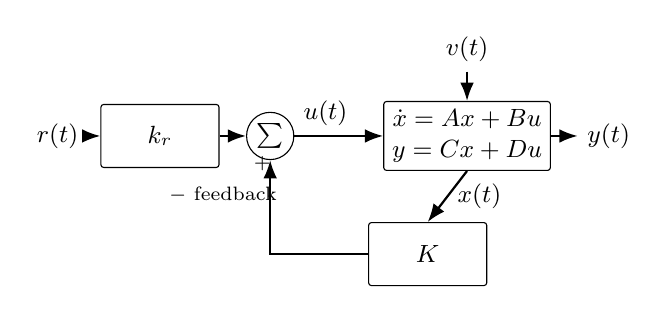
\begin{tikzpicture}[>=Latex,every node/.style={font=\small}]
			\node (r) at (-4.8,0) {$r(t)$};
			\node[ctlblock] (kr) at (-3.5,0) {$k_r$};
			\node[sumj] (sum) at (-2.1,0) {$\sum$};
			\node[ctlblock] (plant) at (0.4,0) {$\dot{x}=Ax+Bu$\\$y=Cx+Du$};
			\node (y) at (2.2,0) {$y(t)$};
			\node[ctlblock] (k) at (-0.1,-1.5) {$K$};
			\node (v) at (0.4,1.1) {$v(t)$};
			\draw[signal] (r) -- (kr);
			\draw[signal] (kr) -- (sum);
			\draw[signal] (sum) -- node[above,pos=0.35] {$u(t)$} (plant);
			\draw[signal] (plant) -- (y);
			\draw[signal] (plant.south) -- node[right] {$x(t)$} (k.north);
			\draw[signal] (k.west) -| (sum.south);
			\draw[signal] (v) -- (plant.north);
			\node[font=\scriptsize] at (-2.2,-0.35) {$+$};
			\node[font=\scriptsize] at (-2.7,-0.75) {$-$ feedback};
		\end{tikzpicture}
		\caption{State-feedback architecture with reference prefilter and input disturbance.}
		\label{fig:state-feedback-architecture}
	\end{figure}
	\textit{(Block diagram representation of full-state feedback with reference precompensation and input disturbance).}
	\paragraph{Closed-Loop Governing Equations}
	Assuming all states $x(t) \in \mathbb{R}^n$ can be measured directly, the control law is defined as: \[
	u(t) = -Kx(t) + k_r r(t) + v(t)
	\] where $K = \begin{bmatrix} K_1 & K_2 & \dots & K_n \end{bmatrix} \in \mathbb{R}^{1 \times n}$ is the state feedback gain vector, and $k_r$ is the reference feedforward gain.
	Substituting $u(t)$ into the open-loop dynamics yields: \[
	\dot{x}(t) = Ax(t) + B\left( -Kx(t) + k_r r(t) + v(t) \right) = (A - BK)x(t) + B k_r r(t) + B v(t)
	\] \[
	y(t) = Cx(t) + D\left( -Kx(t) + k_r r(t) + v(t) \right) = (C - DK)x(t) + D k_r r(t) + D v(t)
	\]
	\paragraph{Stability Criterion}
	The unforced stability and natural transient modes of the closed-loop system are governed entirely by the eigenvalues of the closed-loop system matrix $(A - BK)$: \[
	\det(sI - (A - BK)) = 0
	\] The closed-loop system is internally stable if and only if all eigenvalues of $(A - BK)$ lie strictly in the open left-half complex plane: \[
	\text{Re}(\lambda_i(A - BK)) < 0, \quad \forall i \in \{1, 2, \dots, n\}
	\]
	\paragraph{The Fundamental Theorem of Pole Placement}
	\begin{quote}
		\textbf{Theorem:} If the open-loop system pair $(A, B)$ is reachable, then for any arbitrary monic target polynomial of degree $n$ with real coefficients: \[
		\alpha_d(s) = s^n + t_1 s^{n-1} + t_2 s^{n-2} + \dots + t_{n-1}s + t_n
		\] there exists a unique state feedback gain vector $K$ such that the closed-loop characteristic polynomial matches the target polynomial identically: \[
		\det(sI - (A - BK)) = \alpha_d(s)
		\] This guarantees that all $n$ closed-loop eigenvalues can be placed at arbitrary pre-selected locations in the complex plane (with complex poles occurring in conjugate pairs).
	\end{quote}
	
	\subsection{Systematic Pole Placement Techniques}
	\subsubsection{Revision Checklist}
	\begin{itemize}
		\item[$\square$]
		\textbf{Synthesize feedback gains directly} using Reachable Canonical Form: $\tilde{K}_i = t_i - a_i$.
		\item[$\square$]
		\textbf{State and apply Ackermann’s Formula} for single-input pole placement: $K = \begin{bmatrix} 0 & \dots & 0 & 1 \end{bmatrix} W_r^{-1} \alpha_d(A)$.
		\item[$\square$]
		\textbf{Distinguish between the numerical algorithms} in MATLAB (\texttt{acker} vs. \texttt{place}).
		\item[$\square$]
		\textbf{Identify the eigenvalue multiplicity limitation} of the robust \texttt{place} command.
	\end{itemize}
	
	\subsubsection{Core Concepts \& Formulations}
	\begin{figure}[H]
		\centering
		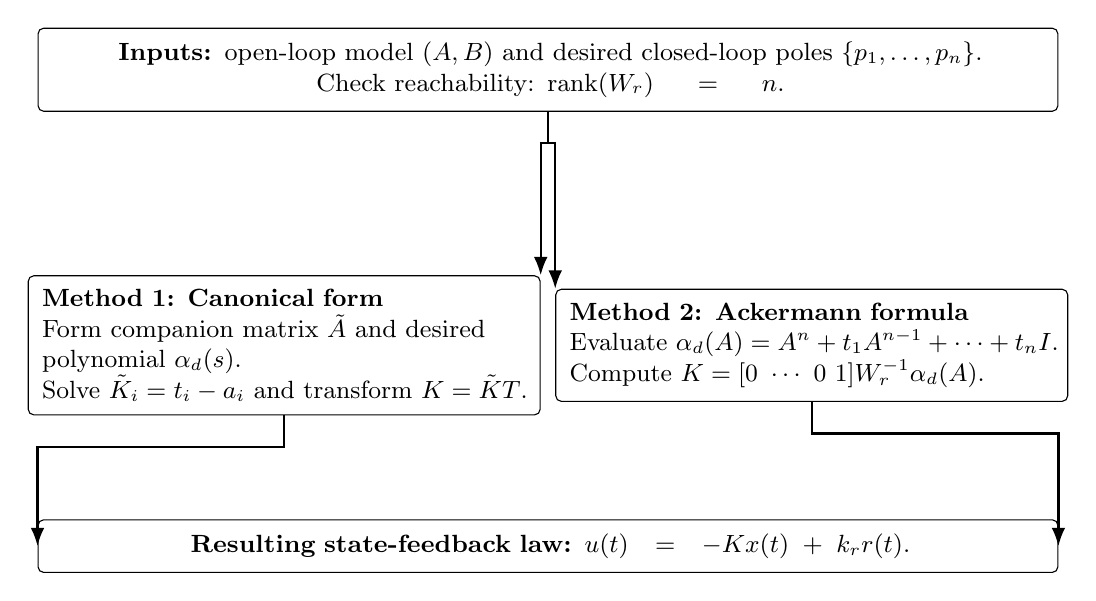
\begin{tikzpicture}[>=Latex,every node/.style={font=\small}]
			\node[flowbox] (start) at (0,4.3) {\textbf{Inputs:} open-loop model $(A,B)$ and desired closed-loop poles $\{p_1,\ldots,p_n\}$.\\Check reachability: $\operatorname{rank}(W_r)=n$.};
			\node[flowboxleft] (m1) at (-3.35,0.8) {\textbf{Method 1: Canonical form}\\Form companion matrix $\tilde A$ and desired polynomial $\alpha_d(s)$.\\Solve $\tilde K_i=t_i-a_i$ and transform $K=\tilde K T$.};
			\node[flowboxleft] (m2) at (3.35,0.8) {\textbf{Method 2: Ackermann formula}\\Evaluate $\alpha_d(A)=A^n+t_1A^{n-1}+\cdots+t_nI$.\\Compute $K=[0\ \cdots\ 0\ 1]W_r^{-1}\alpha_d(A)$.};
			\node[flowbox] (result) at (0,-1.75) {\textbf{Resulting state-feedback law:} $u(t)=-Kx(t)+k_r r(t)$.};
			\draw[flowarrow] (start.south) -- ++(0,-4mm) -| (m1.north east);
			\draw[flowarrow] (start.south) -- ++(0,-4mm) -| (m2.north west);
			\draw[flowarrow] (m1.south) -- ++(0,-4mm) -| (result.west);
			\draw[flowarrow] (m2.south) -- ++(0,-4mm) -| (result.east);
		\end{tikzpicture}
		\caption{Workflow for state-feedback pole placement using canonical form or Ackermann's formula.}
		\label{fig:state-feedback-design-workflow}
	\end{figure}
	
	\subsubsection{Method 1: Pole Placement via Reachable Canonical Form}
	\begin{enumerate}
		\item
		\textbf{Find Open-Loop Polynomial:} Compute the characteristic polynomial of $A$: \[
		\det(sI - A) = s^n + a_1 s^{n-1} + \dots + a_{n-1}s + a_n
		\]
		\item
		\textbf{Construct Target Polynomial:} From the desired closed-loop poles ${p_1, p_2, \dots, p_n}$, expand the target polynomial: \[
		\alpha_d(s) = \prod_{k=1}^n (s - p_k) = s^n + t_1 s^{n-1} + \dots + t_{n-1}s + t_n
		\]
		\item
		\textbf{Calculate Gains in Canonical Coordinates:} In reachable canonical coordinates $z$, the control law $\tilde{u} = -\tilde{K}z$ modifies only the first row of $\tilde{A}$: \[
		\tilde{A} - \tilde{B}\tilde{K} = \begin{bmatrix} -(a_1 + \tilde{K}_1) & -(a_2 + \tilde{K}_2) & \dots & -(a_n + \tilde{K}_n) \\ 1 & 0 & \dots & 0 \\ \vdots & \ddots & \dots & \vdots \\ 0 & \dots & 1 & 0 \end{bmatrix}
		\] Matching coefficients directly with the target polynomial yields: \[
		\tilde{K}_i = t_i - a_i, \quad i = 1, 2, \dots, n
		\]
		\item
		\textbf{Transform Back to Physical State Coordinates:} Since $z = Tx$, the feedback becomes $u = -\tilde{K}z = -\tilde{K}Tx = -Kx$: \[
		K = \tilde{K}T = \tilde{K} (\tilde{W}_r W_r^{-1})
		\]
	\end{enumerate}
	
	\subsubsection{Method 2: Ackermann’s Formula}
	For single-input systems, Ackermann's formula bypasses the explicit construction of the similarity transformation matrix $T$: \[
	K = \begin{bmatrix} 0 & 0 & \dots & 0 & 1 \end{bmatrix} W_r^{-1} \alpha_d(A)
	\] where $\alpha_d(A) \in \mathbb{R}^{n \times n}$ is the matrix evaluation of the desired polynomial: \[
	\alpha_d(A) = A^n + t_1 A^{n-1} + t_2 A^{n-2} + \dots + t_{n-1} A + t_n I
	\]
	\paragraph{Analytical Derivation of Ackermann’s Formula (for $n = 3$)}
	Let $\tilde{A} = A - BK$ represent the closed-loop matrix. By the Cayley-Hamilton theorem, $\tilde{A}$ satisfies its target characteristic equation: \[
	\alpha_d(\tilde{A}) = \tilde{A}^3 + t_1 \tilde{A}^2 + t_2 \tilde{A} + t_3 I = 0
	\]
	Examining successive matrix powers:
	\begin{itemize}
		\item
		$\tilde{A} = A - BK$
		\item
		$\tilde{A}^2 = (A - BK)^2 = A^2 - ABK - BK\tilde{A}$
		\item
		$\tilde{A}^3 = (A - BK)^3 = A^3 - A^2 BK - ABK\tilde{A} - BK\tilde{A}^2$
	\end{itemize}
	Substituting these powers into the polynomial expansion yields: \[
	\alpha_d(\tilde{A}) = \alpha_d(A) - \left[ A^2 BK + ABK\tilde{A} + BK\tilde{A}^2 + t_1(ABK + BK\tilde{A}) + t_2 BK \right] = 0
	\] \[
	\alpha_d(A) = \begin{bmatrix} B & AB & A^2 B \end{bmatrix} \begin{bmatrix} t_2 K + t_1 K\tilde{A} + K\tilde{A}^2 \\ t_1 K + K\tilde{A} \\ K \end{bmatrix} = W_r \begin{bmatrix} * \\ * \\ K \end{bmatrix}
	\]
	Premultiplying both sides by $W_r^{-1}$: \[
	W_r^{-1} \alpha_d(A) = \begin{bmatrix} * \\ * \\ K \end{bmatrix}
	\] Premultiplying by the row selection vector $\begin{bmatrix} 0 & 0 & 1 \end{bmatrix}$ isolates the gain vector $K$: \[
	K = \begin{bmatrix} 0 & 0 & 1 \end{bmatrix} W_r^{-1} \alpha_d(A)
	\]
	
	\subsubsection{Computational Pole Placement in MATLAB}
	\begin{itemize}
		\item
		\texttt{K = acker(A, B, p)}: Direct implementation of Ackermann's formula. While versatile for single-input systems with repeated eigenvalues ($p_i = p_j$), it relies on inverting $W_r$ and evaluating high matrix powers $A^n$, making it numerically ill-conditioned for system orders $n > 10$ or weakly reachable plants.
		\item
		\texttt{K = place(A, B, p)}: Employs the numerically robust Kautsky-Nichols-Van Dooren algorithm. Applicable to multi-input systems, it optimizes eigenvector conditioning to maximize stability margins.
		\begin{itemize}
			\item
			\textit{Constraint:} The multiplicity of any desired closed-loop pole cannot exceed the number of control inputs ($\text{multiplicity}(p_i) \le \text{rank}(B)$). For SISO plants, \textbf{all desired closed-loop poles must be strictly distinct}.
		\end{itemize}
	\end{itemize}
	
	\subsection{Reference Precompensation ($k_r$) \& Integral Augmentation}
	\subsubsection{Revision Checklist}
	\begin{itemize}
		\item[$\square$]
		\textbf{Derive the reference precompensation gain} $k_r$ to ensure unity steady-state closed-loop gain ($y_{ss} = r_{ss}$).
		\item[$\square$]
		\textbf{Explain why static feedforward gain $k_r$ fails to reject} constant input disturbances $v_0$ or survive plant parameter drift.
		\item[$\square$]
		\textbf{Formulate the state-space equations for an augmented system} incorporating an integral tracking error state $x_i$.
		\item[$\square$]
		\textbf{State the reachability condition} for the integral-augmented system matrix.
	\end{itemize}
	
	\subsubsection{Core Concepts \& Formulations}
	\paragraph{Derivation of Precompensation Gain $k_r$}
	Full-state feedback regulates states toward zero. To track a non-zero reference setpoint $r(t)$, the reference signal is injected through a scaling gain $k_r$: \[
	\dot{x}(t) = (A - BK)x(t) + B k_r r(t), \quad y(t) = Cx(t) \quad (\text{assuming } D = 0)
	\]
	At steady state under a constant step command $r(t) = r_{ss}$, state derivatives settle to zero ($\dot{x}_{ss} = 0$): \[
	0 = (A - BK)x_{ss} + B k_r r_{ss} \implies x_{ss} = -(A - BK)^{-1} B k_r r_{ss}
	\] \[
	y_{ss} = C x_{ss} = -C (A - BK)^{-1} B k_r r_{ss}
	\]
	To guarantee zero steady-state tracking error ($y_{ss} = r_{ss}$), the closed-loop DC gain must equal unity: \[
	\frac{y_{ss}}{r_{ss}} = 1 \implies k_r = -\frac{1}{C(A - BK)^{-1}B}
	\] \textit{Physical Meaning:} The precompensation gain $k_r$ is precisely the reciprocal of the closed-loop system's zero-frequency (DC) transmission gain.
	\paragraph{Vulnerability to Disturbances and Model Mismatch}
	If a constant input disturbance $v(t) = v_0$ acts on the plant input, the steady-state output becomes: \[
	y_{ss} = -C(A - BK)^{-1}B (k_r r_{ss} + v_0) = r_{ss} - C(A - BK)^{-1}B v_0
	\] Because $k_r$ acts purely as an open-loop feedforward gain, it \textbf{cannot eliminate steady-state offsets caused by unmodeled plant parameter variations or constant load disturbances}.
	\paragraph{Robust Tracking via Integral State Augmentation}
	To eliminate steady-state tracking error under constant disturbances without precise plant model calibration, introduce an integrator state $x_i(t)$ that continuously accumulates the tracking error $e_y(t) = r(t) - y(t)$: \[
	\dot{x}_i(t) = r(t) - y(t) = r(t) - Cx(t)
	\]
	Constructing the augmented state vector $x_a(t) = \begin{bmatrix} x(t) \\ x_i(t) \end{bmatrix} \in \mathbb{R}^{n+1}$ yields: \[
	\begin{bmatrix} \dot{x}(t) \\ \dot{x}_i(t) \end{bmatrix} = \begin{bmatrix} A & 0 \\ -C & 0 \end{bmatrix} \begin{bmatrix} x(t) \\ x_i(t) \end{bmatrix} + \begin{bmatrix} B \\ 0 \end{bmatrix} u(t) + \begin{bmatrix} 0 \\ 1 \end{bmatrix} r(t)
	\]
	The augmented state feedback control law becomes: \[
	u(t) = -Kx(t) - K_i x_i(t) = -\begin{bmatrix} K & K_i \end{bmatrix} \begin{bmatrix} x(t) \\ x_i(t) \end{bmatrix}
	\]
	The resulting augmented closed-loop system matrix is: \[
	A_a - B_a K_a = \begin{bmatrix} A - BK & -B K_i \\ -C & 0 \end{bmatrix}
	\]
	\begin{itemize}
		\item
		\textbf{Reachability Condition for the Augmented System:} The augmented $(n+1)$-dimensional system is reachable if and only if the open-loop plant $(A, B)$ is reachable and the plant transfer function has no transmission zero at $s = 0$: \[
		\det \begin{bmatrix} A & B \\ -C & 0 \end{bmatrix} \neq 0 \iff P(0) = -CA^{-1}B \neq 0
		\] When this rank condition holds, the feedback gain vector $\begin{bmatrix} K & K_i \end{bmatrix}$ places all $n+1$ closed-loop eigenvalues in the open left-half plane, guaranteeing asymptotic disturbance rejection ($y_{ss} = r_{ss}$) even under plant parameter uncertainty.
	\end{itemize}
	
	\subsection{Practical Implementation Trade-offs \& Actuator Authority}
	\subsubsection{Revision Checklist}
	\begin{itemize}
		\item[$\square$]
		\textbf{Quantify the trade-off} between closed-loop response speed and actuator control effort ($|u(t)|$).
		\item[$\square$]
		\textbf{Explain how aggressive pole placement amplifies sensor noise} and induces high-frequency chatter.
		\item[$\square$]
		\textbf{Use dominant second-order pole metrics} ($\zeta, \omega_n, T_s, M_p$) to select target closed-loop pole locations.
		\item[$\square$]
		\textbf{Place non-dominant poles sufficiently far into the left-half plane} (or near open-loop zeros) to preserve the validity of low-order approximations.
	\end{itemize}
	
	\subsubsection{Core Concepts \& Engineering Trade-offs}
	\paragraph{The Control Authority vs. Speed Dilemma}
	While the Pole Placement Theorem proves that eigenvalues can mathematically be shifted anywhere in the complex plane, physical hardware imposes strict operational boundaries:
	\begin{center}\small\begin{tabularx}{\textwidth}{*{3}{Y}}
			\toprule
			\textbf{Performance Metric} & \textbf{Moving Closed-Loop Poles Farther Left ($\text{Re}(p_k) \ll 0$)} & \textbf{Moving Closed-Loop Poles Closer to the Imaginary Axis} \\
			\midrule
			\textbf{Response Speed ($T_r, T_s$)} & \textbf{Significantly faster:} Rapid transient decay and short settling times. & \textbf{Slower:} Sluggish settling time, extended transient envelopes. \\
			\textbf{Control Signal Magnitude ($\lvert u(t)\rvert$)} & \textbf{Large:} Requires high peak control effort and aggressive actuator authority. & \textbf{Small:} Gentle, low-amplitude control effort. \\
			\textbf{Actuator Saturation Risk} & \textbf{Severe:} Exceeds actuator voltage/torque/force limits, leading to windup or instability. & \textbf{Minimal:} System operates cleanly within its linear dynamic range. \\
			\textbf{Sensor Noise Amplification} & \textbf{High:} High-gain feedback amplifies high-frequency measurement noise into the actuators. & \textbf{Low:} Natural low-pass filtering effect attenuates high-frequency sensor noise. \\
			\bottomrule
	\end{tabularx}\end{center}
	\paragraph{Pole Selection via Second-Order Dominant Approximations}
	To balance performance against control effort, designers typically specify a pair of dominant complex-conjugate poles based on transient response requirements: \[
	p_{1,2} = -\zeta \omega_n \pm j \omega_n \sqrt{1 - \zeta^2}
	\]
	\begin{itemize}
		\item
		\textbf{Damping Ratio ($\zeta$):} Dictates percentage overshoot ($M_p$): \[
		M_p = \exp\left( -\frac{\pi \zeta}{\sqrt{1 - \zeta^2}} \right) \iff \zeta = \frac{-\ln(M_p)}{\sqrt{\pi^2 + \ln^2(M_p)}}
		\]
		\item
		\textbf{Natural Frequency ($\omega_n$):} Governs settling time ($T_s$) and rise time: \[
		T_s \approx \frac{4}{\zeta \omega_n} \quad (\text{for a } 2\% \text{ settling criterion})
		\]
	\end{itemize}
	\paragraph{Placement of Non-Dominant Poles}
	For an $n$-th order system ($n > 2$), the remaining $n - 2$ poles must not alter the transient performance governed by the dominant pair:
	\begin{itemize}
		\item
		\textbf{5x to 10x Rule:} Place non-dominant poles \textbf{5 to 10 times farther to the left} than the real part of the dominant complex poles ($|\text{Re}(p_{\text{non-dom}})| \ge 5 |\zeta \omega_n|$). This ensures their exponential modes decay rapidly, making them negligible in the transient response.
		\item
		\textbf{Zero Cancellation:} Alternatively, place non-dominant poles near open-loop plant zeros to minimize their residue and dynamic contribution to the step response.
	\end{itemize}
	
	\subsection{Summary Comparison of Week 8 State Feedback Properties}
	\begin{center}\small\begin{tabularx}{\textwidth}{*{3}{Y}}
			\toprule
			\textbf{Feature / Concept} & \textbf{Governing Formula / Expression} & \textbf{Physical \& Control System Meaning} \\
			\midrule
			\textbf{Reachability Matrix} & $W_r = \begin{bmatrix} B & AB & \dots & A^{n-1}B \end{bmatrix}$ & Matrix spanning all directions in state space accessible via the actuator. \\
			\textbf{Rank Condition} & $\text{rank}(W_r) = n \iff \det(W_r) \neq 0$ & Necessary and sufficient condition for arbitrary eigenvalue assignment. \\
			\textbf{Reachable Canonical Form} & $\tilde{A}_{\text{comp}},\; \tilde{B} = \begin{bmatrix} 1 & 0 & \dots & 0 \end{bmatrix}^T$ & Form where characteristic coefficients appear directly in the first row. \\
			\textbf{State Feedback Control Law} & $u(t) = -Kx(t) + k_r r(t)$ & Linear mapping from full state vector to control signal (note minus sign). \\
			\textbf{Closed-Loop Dynamics} & $\dot{x} = (A - BK)x + B k_r r$ & Modifies system modes to the eigenvalues of $(A - BK)$. \\
			\textbf{Canonical Pole Placement} & $\tilde{K}_i = t_i - a_i, \quad K = \tilde{K}\tilde{W}_r W_r^{-1}$ & Direct algebraic coefficient matching in canonical coordinates. \\
			\textbf{Ackermann’s Formula} & $K = \begin{bmatrix} 0 & \dots & 1 \end{bmatrix} W_r^{-1} \alpha_d(A)$ & Direct computational formula for single-input state feedback gain. \\
			\textbf{Precompensation Gain} & $k_r = -[C(A - BK)^{-1}B]^{-1}$ & Feedforward reference scaling enforcing unit closed-loop DC gain ($y_{ss} = r_{ss}$). \\
			\textbf{Integral Augmentation} & $\dot{x}_i = r - y,\; u = -Kx - K_i x_i$ & Adds internal error integration to reject constant input disturbances. \\
			\bottomrule
	\end{tabularx}\end{center}
	
	\newpage
	\section{Output feedback}

	
	\subsection{The Output Feedback Architecture \& Need for Estimation}
	\subsubsection{Revision Checklist}
	\begin{itemize}
		\item[$\square$]
		\textbf{Explain why full-state feedback} ($u = -Kx$) is often impractical in physical engineering systems.
		\item[$\square$]
		\textbf{Formulate the open-loop state estimator} (copying the plant model) and state its governing differential equation.
		\item[$\square$]
		\textbf{Derive the estimation error dynamics} for the open-loop estimator and explain why open-loop estimation fails for unstable or weakly damped plants.
		\item[$\square$]
		\textbf{Define the general dynamic output feedback architecture} combining a state estimator with state feedback gains.
	\end{itemize}
	
	\subsubsection{Core Concepts \& Formulations}
	\paragraph{Limitations of Direct Full-State Feedback}
	Full-state feedback ($u(t) = -Kx(t) + k_r r(t)$) assumes all $n$ internal state variables are directly accessible via sensors. In practical engineering implementations:
	\begin{itemize}
		\item
		Physical sensors for every state may be prohibitively expensive, add unacceptable weight, or reduce system reliability.
		\item
		Certain internal dynamic states cannot be physically accessed or measured directly by any sensor.
		\item
		Sensor measurements introduce high-frequency electrical noise that corrupts state derivatives.
	\end{itemize}
	To resolve this, an \textbf{output feedback architecture} is employed: an auxiliary dynamic system called a \textbf{state estimator (observer)} reconstructs an estimate of the state vector $\hat{x}(t) \in \mathbb{R}^n$ using only the applied input $u(t)$ and the measured output $y(t)$.
	\begin{figure}[H]
		\centering
		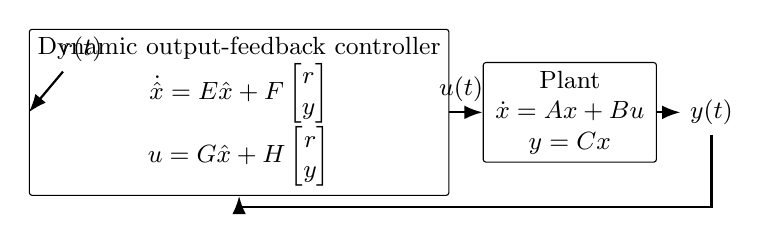
\begin{tikzpicture}[>=Latex,every node/.style={font=\small}]
			\node[ctlwide,minimum width=47mm,minimum height=19mm] (ctrl) at (0,0) {Dynamic output-feedback controller\\$\dot{\hat{x}}=E\hat{x}+F\begin{bmatrix}r\\y\end{bmatrix}$\\$u=G\hat{x}+H\begin{bmatrix}r\\y\end{bmatrix}$};
			\node[ctlwide] (plant) at (4.2,0) {Plant\\$\dot{x}=Ax+Bu$\\$y=Cx$};
			\node (r) at (-2.0,0.8) {$r(t)$};
			\node (y) at (6.0,0) {$y(t)$};
			\draw[signal] (r) -- (ctrl.west);
			\draw[signal] (ctrl.east) -- node[above,pos=0.35] {$u(t)$} (plant.west);
			\draw[signal] (plant.east) -- (y);
			\draw[signal] (y) -- ++(0,-1.2) -| (ctrl.south);
		\end{tikzpicture}
		\caption{Dynamic output-feedback controller coupled to a state-space plant.}
		\label{fig:dynamic-output-feedback}
	\end{figure}
	\textit{(General structure of a dynamic output feedback controller).}
	\paragraph{The Open-Loop Estimator ("Copying the Plant")}
	The simplest state estimator is an open-loop software simulator that mirrors the nominal plant dynamics driven by the known input $u(t)$: \[
	\dot{\hat{x}}(t) = A\hat{x}(t) + Bu(t), \quad \hat{x}(0) = \hat{x}_0
	\]
	Defining the state estimation error as $\tilde{x}(t) = x(t) - \hat{x}(t)$: \[
	\dot{\tilde{x}}(t) = \dot{x}(t) - \dot{\hat{x}}(t) = (Ax(t) + Bu(t)) - (A\hat{x}(t) + Bu(t)) = A\tilde{x}(t)
	\] \[
	\tilde{x}(t) = e^{At}\tilde{x}(0)
	\]
	\textbf{Why Open-Loop Estimation Fails:}
	\begin{enumerate}
		\item
		\textbf{Unstable Plants:} If the open-loop matrix $A$ has any eigenvalue with $\text{Re}(\lambda) \ge 0$, any initial discrepancy $\tilde{x}(0) \neq 0$ grows exponentially without bound, causing the state estimate to diverge.
		\item
		\textbf{Lack of Tuning Freedom:} Even if the plant is stable ($\text{Re}(\lambda_i) < 0$), the estimation error decays only as fast as the plant's open-loop natural modes. If an eigenvalue lies close to the imaginary axis, convergence is excessively slow.
		\item
		\textbf{Absence of Feedback Correction:} The open-loop estimator completely ignores the measured output $y(t)$, preventing the observer from correcting for disturbances or modeling errors.
	\end{enumerate}
	
	\subsection{Observability: Foundations, Intuition, and Rank Criteria}
	\subsubsection{Revision Checklist}
	\begin{itemize}
		\item[$\square$]
		\textbf{State the formal continuous-time definition of observability} over a finite time interval $[0, T]$.
		\item[$\square$]
		\textbf{Explain the physical intuition of unobservability} using symmetric systems where identical subsystem outputs subtract.
		\item[$\square$]
		\textbf{Derive the Observability Matrix} $W_o$ by differentiating the output trajectory $y(t) = C e^{At} x(0)$.
		\item[$\square$]
		\textbf{State the Observability Rank Condition} and explain why powers higher than $A^{n-1}$ provide no new information via the Cayley-Hamilton theorem.
		\item[$\square$]
		\textbf{Define the unobservable subspace} $\ker(W_o)$ and explain its physical consequences.
	\end{itemize}
	
	\subsubsection{Core Concepts \& Formulations}
	\paragraph{Formal Definition of Observability}
	Consider the linear time-invariant system: \[
	\dot{x}(t) = Ax(t) + Bu(t), \quad y(t) = Cx(t)
	\]
	A continuous-time system is \textbf{observable} if, for any initial state $x(0) \in \mathbb{R}^n$ and any finite time $T > 0$, the initial state $x(0)$ can be uniquely determined from knowledge of the input trajectory $u(t)$ and the output trajectory $y(t)$ measured over the interval $t \in [0, T]$.
	\begin{itemize}
		\item
		If $x(0)$ can be determined, then the current state $x(t)$ can be reconstructed for all $t \ge 0$ by integrating the known dynamics.
		\item
		Because the input $u(t)$ and the input matrices $(A, B)$ are known, the zero-state contribution $\int_0^t C e^{A(t-\tau)} B u(\tau) d\tau$ can be subtracted from $y(t)$. Therefore, observability depends strictly on the autonomous pair $(A, C)$.
	\end{itemize}
	\paragraph{Mechanisms of Unobservability}
	A system is unobservable when certain internal states or natural modes fail to transmit any dynamical signature to the measured output sensors:
	\begin{itemize}
		\item
		\textbf{Symmetric Opposing Dynamics:} If two identical subsystems $S$ with identical initial conditions feed into a summing junction where their outputs subtract ($y = y_1 - y_2$), the net output remains identically zero ($y(t) \equiv 0$) for all time regardless of the magnitude of their shared motion.
		\item
		\textbf{Decoupled States:} If a state coordinate has zero coupling to the output row ($C_i = 0$) and the system dynamics matrix $A$ does not mix that state into observable states, that coordinate cannot be detected from $y(t)$.
	\end{itemize}
	\paragraph{Derivation of the Observability Matrix}
	For an unforced system ($\dot{x} = Ax,\; y = Cx$), the output trajectory is $y(t) = C e^{At} x(0)$. Taking successive time derivatives at $t = 0$: \[
	y(0) = C x(0)
	\] \[
	\dot{y}(0) = C \dot{x}(0) = CA x(0)
	\] \[
	\ddot{y}(0) = CA \dot{x}(0) = CA^2 x(0)
	\] \[
	\vdots
	\] \[
	y^{(n-1)}(0) = CA^{n-1} x(0)
	\]
	Stacking these scalar equations into matrix form yields: \[
	\begin{bmatrix} y(0) \\ \dot{y}(0) \\ \vdots \\ y^{(n-1)}(0) \end{bmatrix} = \begin{bmatrix} C \\ CA \\ \vdots \\ CA^{n-1} \end{bmatrix} x(0) = W_o x(0)
	\]
	By the \textbf{Cayley-Hamilton theorem}, $A^n$ and all higher matrix powers can be expressed as linear combinations of ${I, A, A^2, \dots, A^{n-1}}$. Thus, taking derivatives higher than $n - 1$ produces rows that are linearly dependent on preceding rows, yielding no additional information about $x(0)$.
	\paragraph{The Observability Matrix and Rank Condition}
	The \textbf{Observability Matrix} $W_o$ (or $\mathcal{O}$) is defined as: \[
	W_o = \begin{bmatrix} C \\ CA \\ CA^2 \\ \vdots \\ CA^{n-1} \end{bmatrix} \in \mathbb{R}^{nq \times n}
	\]
	\begin{itemize}
		\item
		\textbf{Observability Rank Condition:} The pair $(A, C)$ is observable if and only if $W_o$ has full column rank: \[
		\text{rank}(W_o) = n
		\]
		\item
		For a \textbf{single-output system} ($q = 1$), $W_o \in \mathbb{R}^{n \times n}$ is square, and the criterion simplifies to: \[
		\det(W_o) \neq 0
		\]
	\end{itemize}
	\paragraph{The Unobservable Subspace}
	If $\text{rank}(W_o) < n$, the nullspace of $W_o$ defines the \textbf{unobservable subspace}: \[
	\mathcal{N}(W_o) = \ker(W_o) = \{ x_0 \in \mathbb{R}^n \mid W_o x_0 = 0 \}
	\] For any initial state $x(0) \in \ker(W_o)$, the output trajectory is identically zero ($y(t) = C e^{At} x(0) \equiv 0$) for all $t \ge 0$. The sensors are completely blind to any dynamic mode residing within this subspace.
	
	\subsection{Controllability-Observability Duality \& Observable Canonical Form}
	\subsubsection{Revision Checklist}
	\begin{itemize}
		\item[$\square$]
		\textbf{State the Principle of Duality} connecting reachability (controllability) and observability.
		\item[$\square$]
		\textbf{Prove duality algebraically} by showing $W_o(A^T, C^T) = W_r(A, C^T)^T$.
		\item[$\square$]
		\textbf{Construct the Duality Table} showing the mathematical mapping $(A, B, K) \longleftrightarrow (A^T, C^T, L^T)$.
		\item[$\square$]
		\textbf{Write down the companion matrix structure} for Observable Canonical Form.
		\item[$\square$]
		\textbf{Show that observable canonical form} is the dual transpose of reachable canonical form.
	\end{itemize}
	
	\subsubsection{Core Concepts \& Formulations}
	\paragraph{The Principle of Duality}
	There exists a direct mathematical equivalence between the state controllability of a system and the observability of a dual transposed system: \[
	\text{Pair } (A, B) \text{ is reachable} \iff \text{Pair } (A^T, B^T) \text{ is observable}
	\] \[
	\text{Pair } (A, C) \text{ is observable} \iff \text{Pair } (A^T, C^T) \text{ is reachable}
	\]
	\paragraph{Algebraic Proof of Duality}
	Evaluating the observability matrix of the dual pair $(A^T, B^T)$: \[
	W_o(A^T, B^T) = \begin{bmatrix} B^T \\ B^T A^T \\ \vdots \\ B^T (A^T)^{n-1} \end{bmatrix} = \begin{bmatrix} B^T \\ (AB)^T \\ \vdots \\ (A^{n-1}B)^T \end{bmatrix} = \begin{bmatrix} B & AB & \dots & A^{n-1}B \end{bmatrix}^T = W_r(A, B)^T
	\]
	Because the rank of a matrix equals the rank of its transpose ($\text{rank}(W_o) = \text{rank}(W_r^T) = \text{rank}(W_r)$) and $\det(W_o) = \det(W_r^T) = \det(W_r)$, the pair $(A, B)$ is reachable if and only if $(A^T, B^T)$ is observable.
	\paragraph{Mathematical Duality Mapping}
	Because of duality, any theorem, algorithm, or software function developed for state feedback controller design applies directly to state observer design:
	\begin{center}\small\begin{tabularx}{\textwidth}{*{2}{Y}}
			\toprule
			\textbf{Reachability / Controller Design ($u = -Kx$)} & \textbf{Observability / Observer Design ($\dot{\hat{x}} = (A-LC)\hat{x} + \dots$)} \\
			\midrule
			Dynamics Matrix: $A$ & Dynamics Matrix: $A^T$ \\
			Input Matrix: $B$ & Output Matrix: $C^T$ \\
			Reachability Matrix: $W_r = [B ; AB ; \dots ; A^{n-1}B]$ & Transposed Observability Matrix: $W_o^T = [C^T ; A^TC^T ; \dots ; (A^T)^{n-1}C^T]$ \\
			Controller Feedback Gain: $K$ & Transposed Observer Gain: $L^T$ \\
			Closed-Loop Matrix: $(A - BK)$ & Error Dynamics Matrix Transpose: $(A - LC)^T = (A^T - C^T L^T)$ \\
			Characteristic Equation: $\det(sI - (A - BK)) = 0$ & Characteristic Equation: $\det(sI - (A - LC)) = 0$ \\
			\bottomrule
	\end{tabularx}\end{center}
	\paragraph{Observable Canonical Form}
	A single-output system with open-loop characteristic polynomial $\det(sI - A) = s^n + a_1 s^{n-1} + \dots + a_n$ is in \textbf{Observable Canonical Form} if its matrices take the structure: \[
	A_{\text{obs}} = \begin{bmatrix} -a_1 & 1 & 0 & \dots & 0 \\ -a_2 & 0 & 1 & \dots & 0 \\ \vdots & \vdots & \vdots & \ddots & \vdots \\ -a_{n-1} & 0 & 0 & \dots & 1 \\ -a_n & 0 & 0 & \dots & 0 \end{bmatrix}, \quad C_{\text{obs}} = \begin{bmatrix} 1 & 0 & 0 & \dots & 0 \end{bmatrix}
	\]
	\begin{itemize}
		\item
		\textbf{Dual Relation:} Comparing with Reachable Canonical Form shows that $A_{\text{obs}} = A_{\text{reach}}^T$ and $C_{\text{obs}} = B_{\text{reach}}^T$.
		\item
		Any system in observable canonical form has an upper-triangular observability matrix with ones on the main diagonal, guaranteeing that it is \textbf{inherently observable}.
	\end{itemize}
	
	\subsection{Full-Order Luenberger State Observers}
	\subsubsection{Revision Checklist}
	\begin{itemize}
		\item[$\square$]
		\textbf{Formulate the Luenberger observer state equation} incorporating output error injection.
		\item[$\square$]
		\textbf{Identify the innovation signal} ($y - C\hat{x}$) and explain the role of the observer gain matrix $L$.
		\item[$\square$]
		\textbf{Derive the estimation error dynamics} $\dot{e}(t) = (A - LC)e(t)$.
		\item[$\square$]
		\textbf{Show that the error dynamics are unforced} and completely decoupled from control inputs $u(t)$ and references $r(t)$.
		\item[$\square$]
		\textbf{State the condition for asymptotic estimation error convergence} ($\text{Re}(\lambda_i(A - LC)) < 0$).
	\end{itemize}
	
	\subsubsection{Core Concepts \& Formulations}
	\paragraph{The Luenberger Observer Structure}
	To ensure rapid, stable state reconstruction even for unstable plants, David Luenberger introduced a closed-loop estimator that runs a real-time software model of the plant corrected by an \textbf{innovation term} proportional to the output estimation mismatch:
	\[
	\dot{\hat{x}}(t) = A\hat{x}(t) + Bu(t) + L \left( y(t) - C\hat{x}(t) \right)
	\] \[
	\hat{y}(t) = C\hat{x}(t)
	\]
	Grouping internal feedback terms highlights the closed-loop nature of the estimator: \[
	\dot{\hat{x}}(t) = (A - LC)\hat{x}(t) + Bu(t) + Ly(t)
	\] where $L \in \mathbb{R}^{n \times q}$ is the \textbf{Observer Gain Matrix}.
	\begin{figure}[H]
		\centering
		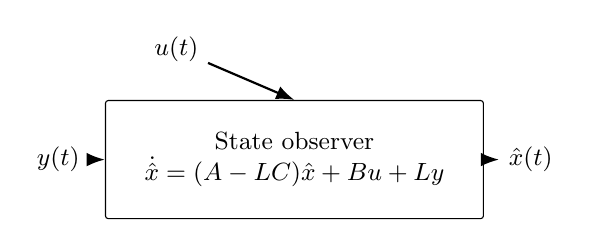
\begin{tikzpicture}[>=Latex,every node/.style={font=\small}]
			\node[ctlwide,minimum width=48mm,minimum height=15mm] (obs) at (0,0) {State observer\\$\dot{\hat{x}}=(A-LC)\hat{x}+Bu+Ly$};
			\node (u) at (-1.5,1.4) {$u(t)$};
			\node (y) at (-3.0,0) {$y(t)$};
			\node (xhat) at (3.0,0) {$\hat{x}(t)$};
			\draw[signal] (u) -- (obs.north);
			\draw[signal] (y) -- (obs.west);
			\draw[signal] (obs.east) -- (xhat);
		\end{tikzpicture}
		\caption{Luenberger observer driven by the plant input and measured output.}
		\label{fig:luenberger-observer}
	\end{figure}
	\textit{(The observer viewed as a dynamic system with inputs $u(t)$ and $y(t)$, and output $\hat{x}(t)$).}
	\paragraph{Derivation of the Estimation Error Dynamics}
	Define the state estimation error as: \[
	e(t) = \tilde{x}(t) = x(t) - \hat{x}(t)
	\]
	Differentiating with respect to time and substituting the plant and observer equations: \[
	\dot{e}(t) = \dot{x}(t) - \dot{\hat{x}}(t)
	\] \[
	\dot{e}(t) = \left( Ax(t) + Bu(t) \right) - \left[ A\hat{x}(t) + Bu(t) + L(Cx(t) - C\hat{x}(t)) \right]
	\] \[
	\dot{e}(t) = A(x(t) - \hat{x}(t)) - LC(x(t) - \hat{x}(t))
	\] \[
	\dot{e}(t) = (A - LC)e(t)
	\]
	The explicit time-domain solution for the error vector is: \[
	e(t) = \exp\left( (A - LC)t \right) e(0)
	\]
	\paragraph{Key Analytical Properties of the Error Dynamics}
	\begin{enumerate}
		\item
		\textbf{Decoupled from Plant Driving Signals:} The control input $u(t)$ and reference $r(t)$ cancel out completely. The error dynamics are strictly autonomous.
		\item
		\textbf{Asymptotic Convergence:} If the gain matrix $L$ is designed such that all eigenvalues of the error dynamics matrix $(A - LC)$ lie strictly in the open left-half complex plane: \[
		\text{Re}(\lambda_i(A - LC)) < 0, \quad \forall i \in \{1, 2, \dots, n\}
		\] then the estimation error decays asymptotically to zero ($\lim_{t \to \infty} e(t) = 0$) regardless of the initial mismatch $\hat{x}(0) \neq x(0)$.
		\item
		\textbf{Eigenvalue Assignment Freedom:} If $(A, C)$ is observable, the eigenvalues of $(A - LC)$ can be placed at arbitrary locations in the complex plane (with complex poles in conjugate pairs).
	\end{enumerate}
	
	\subsection{Systematic Observer Gain Synthesis}
	\subsubsection{Revision Checklist}
	\begin{itemize}
		\item[$\square$]
		\textbf{Synthesize observer gains} in Observable Canonical Form by direct coefficient matching: $L_i = \beta_i - a_i$.
		\item[$\square$]
		\textbf{State and apply Ackermann’s Formula for Observers}: $L = \alpha_o(A) W_o^{-1} \begin{bmatrix} 0 & \dots & 0 & 1 \end{bmatrix}^T$.
		\item[$\square$]
		\textbf{Utilize MATLAB dual syntax} (\texttt{acker(A', C', p)'} and \texttt{place(A', C', p)'}) for observer computation.
		\item[$\square$]
		\textbf{Apply the bandwidth rule of thumb}: placing observer poles 2 to 5 times (or 2 to 10 times) faster than controller poles.
		\item[$\square$]
		\textbf{Quantify the sensor noise sensitivity trade-off} when moving observer poles aggressively to the left.
	\end{itemize}
	
	\subsubsection{Core Concepts \& Formulations}
	\begin{figure}[H]
		\centering
		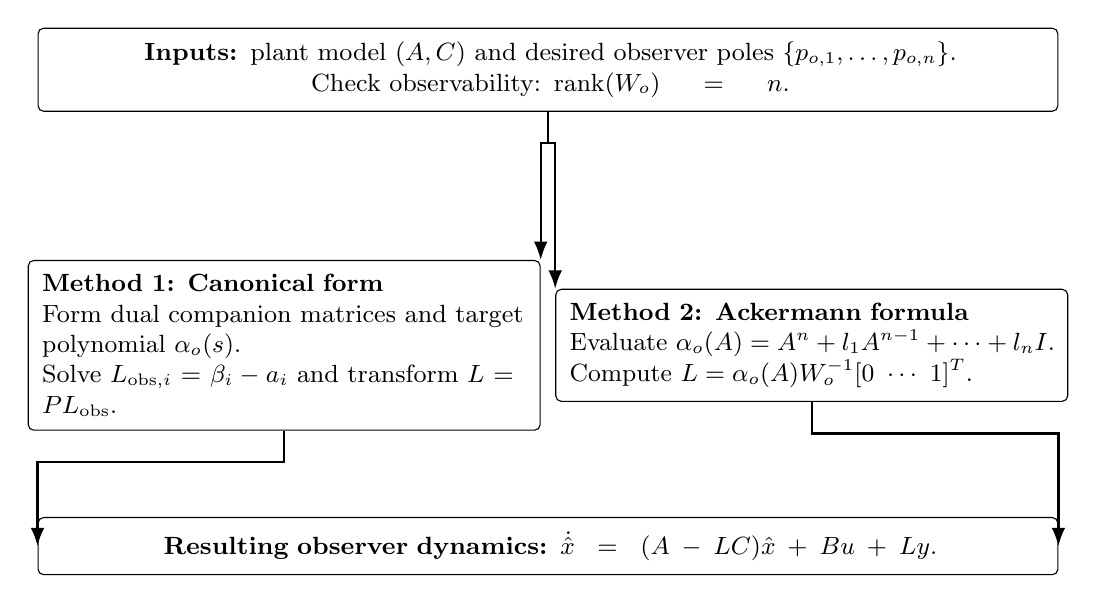
\begin{tikzpicture}[>=Latex,every node/.style={font=\small}]
			\node[flowbox] (start) at (0,4.3) {\textbf{Inputs:} plant model $(A,C)$ and desired observer poles $\{p_{o,1},\ldots,p_{o,n}\}$.\\Check observability: $\operatorname{rank}(W_o)=n$.};
			\node[flowboxleft] (m1) at (-3.35,0.8) {\textbf{Method 1: Canonical form}\\Form dual companion matrices and target polynomial $\alpha_o(s)$.\\Solve $L_{\mathrm{obs},i}=\beta_i-a_i$ and transform $L=P L_{\mathrm{obs}}$.};
			\node[flowboxleft] (m2) at (3.35,0.8) {\textbf{Method 2: Ackermann formula}\\Evaluate $\alpha_o(A)=A^n+l_1A^{n-1}+\cdots+l_nI$.\\Compute $L=\alpha_o(A)W_o^{-1}[0\ \cdots\ 1]^T$.};
			\node[flowbox] (result) at (0,-1.75) {\textbf{Resulting observer dynamics:} $\dot{\hat{x}}=(A-LC)\hat{x}+Bu+Ly$.};
			\draw[flowarrow] (start.south) -- ++(0,-4mm) -| (m1.north east);
			\draw[flowarrow] (start.south) -- ++(0,-4mm) -| (m2.north west);
			\draw[flowarrow] (m1.south) -- ++(0,-4mm) -| (result.west);
			\draw[flowarrow] (m2.south) -- ++(0,-4mm) -| (result.east);
		\end{tikzpicture}
		\caption{Workflow for observer pole placement.}
		\label{fig:observer-design-workflow}
	\end{figure}
	
	\subsubsection{Method 1: Synthesis in Observable Canonical Form}
	\begin{enumerate}
		\item
		Compute the open-loop characteristic polynomial: $\det(sI - A) = s^n + a_1 s^{n-1} + \dots + a_n$.
		\item
		Define the desired observer characteristic polynomial from target roots ${p_{o,1}, \dots, p_{o,n}}$: \[
		\alpha_o(s) = (s - p_{o,1})(s - p_{o,2})\dots(s - p_{o,n}) = s^n + \beta_1 s^{n-1} + \dots + \beta_n
		\]
		\item
		In observable canonical form, $A_{\text{obs}} - L_{\text{obs}}C_{\text{obs}}$ modifies only the first column of the matrix: \[
		L_{\text{obs}, i} = \beta_i - a_i, \quad i = 1, 2, \dots, n
		\]
		\item
		Transform back to physical state coordinates using the transformation matrix $P = W_o^{-1} W_{o,\text{obs}}$: \[
		L = P L_{\text{obs}} = W_o^{-1} W_{o,\text{obs}} L_{\text{obs}}
		\]
	\end{enumerate}
	
	\subsubsection{Method 2: Ackermann’s Formula for Observers}
	For single-output observable systems, applying the duality mapping $(A \to A^T, B \to C^T, K \to L^T)$ to controller Ackermann's formula yields: \[
	L^T = \begin{bmatrix} 0 & 0 & \dots & 1 \end{bmatrix} W_r(A^T, C^T)^{-1} \alpha_o(A^T)
	\]
	Taking the transpose of both sides (and noting that $W_r(A^T, C^T)^T = W_o(A, C)$ and $\alpha_o(A^T)^T = \alpha_o(A)$) gives: \[
	L = \alpha_o(A) W_o^{-1} \begin{bmatrix} 0 \\ 0 \\ \vdots \\ 1 \end{bmatrix}
	\] where $\alpha_o(A) = A^n + \beta_1 A^{n-1} + \dots + \beta_n I \in \mathbb{R}^{n \times n}$.
	
	\subsubsection{Method 3: Computational Synthesis in MATLAB}
	Using duality, MATLAB's pole-placement functions are called with transposed plant matrices:
	\begin{lstlisting}
		% Single-Output systems (order n <= 10)
		L = acker(A', C', p_obs)';
		
		% Multivariable systems or distinct poles (numerically robust)
		L = place(A', C', p_obs)';
	\end{lstlisting}
	
	\subsubsection{Observer Pole Placement Guidelines \& Engineering Trade-offs}
	The selection of observer poles represents a fundamental trade-off between estimation speed and noise immunity:
	\begin{itemize}
		\item
		\textbf{The Speed Rule of Thumb:} Place observer poles \textbf{2 to 5 times (or 2 to 10 times) farther into the left-half plane} than the closed-loop controller poles: \[
		-\text{Re}(\lambda_{\text{obs}}) > -2\,\text{Re}(\lambda_{\text{ctrl}})
		\] \textit{Physical Reasoning:} The state estimation error must decay significantly faster than the natural response time of the plant. If the observer is too slow, the controller acts on obsolete state estimates, causing phase lag, increased overshoot, and degraded tracking.
		\item
		\textbf{The Sensor Noise Penalty:} Moving observer poles excessively far to the left requires a very large gain vector $L$. If sensor measurements are corrupted by high-frequency noise $w(t)$ ($y_m = Cx + w$), the innovation term feeds noise directly into the estimator: \[
		\dot{\hat{x}} = (A - LC)\hat{x} + Bu + L(Cx + w) = (A - LC)\hat{x} + Bu + LCx + Lw(t)
		\] Excessive observer gains amplify sensor noise, inducing high-frequency chatter in the actuators and driving the plant into actuator saturation.
	\end{itemize}
	
	\subsection{Observer-Based Control \& The Separation Principle}
	\subsubsection{Revision Checklist}
	\begin{itemize}
		\item[$\square$]
		\textbf{Formulate the observer-based control law} $u(t) = -K\hat{x}(t) + k_r r(t)$.
		\item[$\square$]
		\textbf{Construct the $2n$-dimensional composite state vector} combining plant states $x(t)$ and estimation errors $e(t)$.
		\item[$\square$]
		\textbf{Derive the block upper-triangular closed-loop system matrix}: \[
		\begin{bmatrix} A - BK & BK \\ 0 & A - LC \end{bmatrix}
		\]
		\item[$\square$]
		\textbf{Prove the Separation Principle} using the determinant property of block triangular matrices.
		\item[$\square$]
		\textbf{State the operational significance of the Separation Theorem} for control system synthesis.
	\end{itemize}
	
	\subsubsection{Core Concepts \& Formulations}
	\paragraph{Observer-Based Control Architecture}
	When physical states cannot be measured, the control law substitutes the estimated states $\hat{x}(t)$ in place of the true states $x(t)$: \[
	u(t) = -K\hat{x}(t) + k_r r(t)
	\]
	\begin{figure}[H]
		\centering
		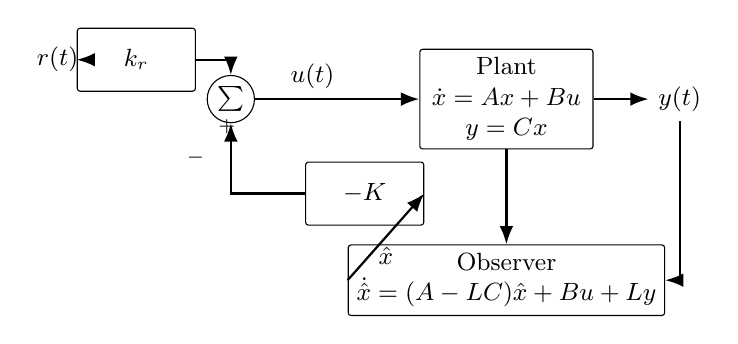
\begin{tikzpicture}[>=Latex,every node/.style={font=\small}]
			\node (r) at (-4.2,0.7) {$r(t)$};
			\node[ctlblock] (kr) at (-3.2,0.7) {$k_r$};
			\node[sumj] (sum) at (-2.0,0.2) {$\sum$};
			\node[ctlblock] (k) at (-0.3,-1.0) {$-K$};
			\node[ctlwide] (plant) at (1.5,0.2) {Plant\\$\dot{x}=Ax+Bu$\\$y=Cx$};
			\node[ctlwide] (obs) at (1.5,-2.1) {Observer\\$\dot{\hat{x}}=(A-LC)\hat{x}+Bu+Ly$};
			\node (y) at (3.7,0.2) {$y(t)$};
			\draw[signal] (r) -- (kr);
			\draw[signal] (kr.east) -| (sum.north);
			\draw[signal] (sum) -- node[above,pos=0.35] {$u(t)$} (plant.west);
			\draw[signal] (plant.east) -- (y);
			\draw[signal] (plant.south) -- (obs.north);
			\draw[signal] (y) |- (obs.east);
			\draw[signal] (obs.west) -- node[below] {$\hat{x}$} (k.east);
			\draw[signal] (k.west) -| (sum.south);
			\node[font=\scriptsize] at (-2.05,-0.15) {$+$};
			\node[font=\scriptsize] at (-2.45,-0.55) {$-$};
		\end{tikzpicture}
		\caption{Observer-based state-feedback controller using estimated state $\hat{x}$.}
		\label{fig:observer-based-controller}
	\end{figure}
	\textit{(Block diagram of the combined observer-controller feedback system).}
	\paragraph{Augmented Closed-Loop State Dynamics}
	Since both the plant and the observer are $n$-th order systems, the overall interconnected closed-loop system is of order $2n$. To analyze its eigenvalues, define the transformed state vector grouping the true state $x(t)$ and the estimation error $e(t) = x(t) - \hat{x}(t)$: \[
	\begin{bmatrix} x(t) \\ e(t) \end{bmatrix} = \begin{bmatrix} I & 0 \\ I & -I \end{bmatrix} \begin{bmatrix} x(t) \\ \hat{x}(t) \end{bmatrix}
	\]
	Express the control law in terms of $x(t)$ and $e(t)$ by substituting $\hat{x} = x - e$: \[
	u(t) = -K(x(t) - e(t)) + k_r r(t) = -Kx(t) + Ke(t) + k_r r(t)
	\]
	Substitute $u(t)$ into the plant state equation: \[
	\dot{x}(t) = Ax(t) + B\left( -Kx(t) + Ke(t) + k_r r(t) \right) = (A - BK)x(t) + BKe(t) + B k_r r(t)
	\]
	Combine this with the autonomous error equation $\dot{e}(t) = (A - LC)e(t)$: \[
	\begin{bmatrix} \dot{x}(t) \\ \dot{e}(t) \end{bmatrix} = \begin{bmatrix} A - BK & BK \\ 0 & A - LC \end{bmatrix} \begin{bmatrix} x(t) \\ e(t) \end{bmatrix} + \begin{bmatrix} B k_r \\ 0 \end{bmatrix} r(t)
	\] \[
	y(t) = \begin{bmatrix} C & 0 \end{bmatrix} \begin{bmatrix} x(t) \\ e(t) \end{bmatrix}
	\]
	\paragraph{Proof of the Separation Principle}
	Because the augmented system matrix is block upper-triangular, its characteristic determinant splits into the product of the determinants of its diagonal blocks: \[
	\det \left( sI - \begin{bmatrix} A - BK & BK \\ 0 & A - LC \end{bmatrix} \right) = \det(sI - (A - BK)) \cdot \det(sI - (A - LC))
	\]
	\begin{quote}
		\textbf{The Separation Principle (Separation Theorem):} The design of the state feedback gain vector $K$ and the observer gain vector $L$ can be carried out \textbf{completely independently}:  1. Compute $K$ assuming all states are directly measured to place the controller poles at $\text{eig}(A - BK)$. 2. Compute $L$ independently to place the observer error poles at $\text{eig}(A - LC)$.  The $2n$ closed-loop eigenvalues of the combined system consist simply of the \textbf{union of the $n$ controller eigenvalues and the $n$ observer eigenvalues}: \[
		\Lambda_{\text{closed-loop}} = \text{eig}(A - BK) \cup \text{eig}(A - LC)
		\]
	\end{quote}
	
	\subsection{Frequency-Domain Realization \& Transfer Functions}
	\subsubsection{Revision Checklist}
	\begin{itemize}
		\item[$\square$]
		\textbf{Eliminate the observer internal state} $\hat{x}$ to derive the controller transfer function $C_{\text{ctrl}}(s) = \frac{U(s)}{-Y(s)}$.
		\item[$\square$]
		\textbf{Formulate the Two-Degree-of-Freedom (2-DOF)} controller equations relating $U(s)$ to $R(s)$ and $Y(s)$.
		\item[$\square$]
		\textbf{Identify the poles of the dynamic controller} as the eigenvalues of $(A - BK - LC)$.
		\item[$\square$]
		\textbf{Explain why output feedback loses the guaranteed stability margins} (e.g., infinite gain margin, $\pm 60^\circ$ phase margin) of pure state feedback.
	\end{itemize}
	
	\subsubsection{Core Concepts \& Formulations}
	\paragraph{Derivation of the Dynamic Controller Transfer Function}
	To express the observer-based controller as a classical transfer function block, substitute the control law $u(t) = -K\hat{x}(t) + k_r r(t)$ into the observer differential equation: \[
	\dot{\hat{x}}(t) = (A - LC)\hat{x}(t) + B(-K\hat{x}(t) + k_r r(t)) + Ly(t)
	\] \[
	\dot{\hat{x}}(t) = (A - BK - LC)\hat{x}(t) + B k_r r(t) + Ly(t)
	\]
	Taking the Laplace transform with zero initial conditions ($\hat{x}(0) = 0$): \[
	(sI - (A - BK - LC))\hat{X}(s) = B k_r R(s) + L Y(s)
	\] \[
	\hat{X}(s) = (sI - (A - BK - LC))^{-1} B k_r R(s) + (sI - (A - BK - LC))^{-1} L Y(s)
	\]
	Substitute $\hat{X}(s)$ into the control law $U(s) = -K\hat{X}(s) + k_r R(s)$: \[
	U(s) = \left[ k_r - K(sI - A + BK + LC)^{-1} B k_r \right] R(s) - \left[ K(sI - A + BK + LC)^{-1} L \right] Y(s)
	\]
	This produces the \textbf{Two-Degree-of-Freedom (2-DOF)} controller structure: \[
	U(s) = G_{ur}(s)R(s) - C_{\text{ctrl}}(s)Y(s)
	\]
	\begin{figure}[H]
		\centering
		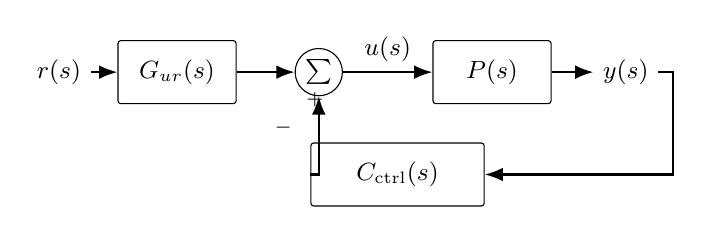
\begin{tikzpicture}[>=Latex,every node/.style={font=\small}]
			\node (r) at (-4.5,0) {$r(s)$};
			\node[ctlblock] (gref) at (-3.0,0) {$G_{ur}(s)$};
			\node[sumj] (sum) at (-1.2,0) {$\sum$};
			\node[ctlblock] (p) at (1.0,0) {$P(s)$};
			\node (y) at (2.7,0) {$y(s)$};
			\node[ctlwide] (c) at (-0.2,-1.3) {$C_{\mathrm{ctrl}}(s)$};
			\draw[signal] (r) -- (gref);
			\draw[signal] (gref) -- (sum);
			\draw[signal] (sum) -- node[above] {$u(s)$} (p);
			\draw[signal] (p) -- (y);
			\draw[signal] (y) -- ++(0.6,0) |- (c.east);
			\draw[signal] (c.west) -| (sum.south);
			\node[font=\scriptsize] at (-1.25,-0.35) {$+$};
			\node[font=\scriptsize] at (-1.65,-0.7) {$-$};
		\end{tikzpicture}
		\caption{Reference-model feedforward path combined with feedback compensation.}
		\label{fig:feedforward-feedback-architecture}
	\end{figure}
	\textit{(Classical 2-DOF unity feedback representation of observer-based control).}
	The feedback compensator transfer function is: \[
	C_{\text{ctrl}}(s) = K \left( sI - (A - BK - LC) \right)^{-1} L
	\]
	\begin{itemize}
		\item
		\textbf{Controller Poles:} The poles of $C_{\text{ctrl}}(s)$ are the eigenvalues of $(A - BK - LC)$. While $(A - BK)$ and $(A - LC)$ are individually designed to be stable, the matrix $(A - BK - LC)$ is not constrained to be stable; therefore, \textbf{an observer-based controller may itself be open-loop unstable} while still stabilizing the plant.
		\item
		\textbf{Loss of Guaranteed Robustness Margins:} Pure Linear Quadratic Regulator (LQR) full-state feedback possesses guaranteed infinite gain margin and at least $\pm 60^\circ$ of phase margin. However, as proven by John Doyle (1978), \textbf{these robust stability margins are completely lost when estimated states $\hat{x}$ from an observer replace physical states}. Consequently, loop transfer recovery (LTR) and frequency-domain margin verification are essential in output feedback design.
	\end{itemize}
	
	\subsection{Optimal Estimation: The Kalman Filter (Preview)}
	\subsubsection{Revision Checklist}
	\begin{itemize}
		\item[$\square$]
		\textbf{Formulate the continuous-time stochastic state-space model} with process disturbance $v(t)$ and measurement noise $w(t)$.
		\item[$\square$]
		\textbf{State the Filter Algebraic Riccati Equation (FARE)} governing optimal error covariance $P$.
		\item[$\square$]
		\textbf{Express the optimal Kalman gain} $L = P C^T R_w^{-1}$.
		\item[$\square$]
		\textbf{Define Linear Quadratic Gaussian (LQG) control} as the combination of LQR state feedback and the Kalman filter.
	\end{itemize}
	
	\subsubsection{Core Concepts \& Formulations}
	\paragraph{Stochastic System Formulation}
	When plant disturbances $v(t)$ and sensor measurement noise $w(t)$ are modeled as zero-mean, uncorrelated Gaussian white noise processes: \[
	\dot{x}(t) = Ax(t) + Bu(t) + v(t), \quad y(t) = Cx(t) + w(t)
	\] \[
	\mathbb{E}[v(t)v^T(\tau)] = R_v \delta(t - \tau), \quad \mathbb{E}[w(t)w^T(\tau)] = R_w \delta(t - \tau), \quad \mathbb{E}[v(t)w^T(\tau)] = 0
	\] where $R_v \ge 0$ is the process noise covariance matrix and $R_w > 0$ is the sensor noise covariance matrix.
	\paragraph{The Kalman-Bucy Filter}
	Rather than choosing observer poles heuristically, the \textbf{Kalman Filter} computes the observer gain $L$ that minimizes the steady-state mean-squared estimation error: \[
	J = \lim_{t \to \infty} \mathbb{E}\left[ |x(t) - \hat{x}(t)|^2 \right] = \text{Tr}(P)
	\]
	The optimal steady-state observer gain is: \[
	L = P C^T R_w^{-1}
	\] where $P = P^T > 0$ is the estimation error covariance matrix ($P = \mathbb{E}[e(t)e^T(t)]$), obtained as the unique positive-definite solution to the \textbf{Filter Algebraic Riccati Equation (FARE)}: \[
	AP + PA^T - PC^T R_w^{-1} C P + R_v = 0
	\]
	In MATLAB, this gain is computed via:
	\begin{lstlisting}
		[L, P] = lqe(A, eye(n), C, Rv, Rw);
	\end{lstlisting}
	Combining LQR state feedback with the Kalman filter forms the \textbf{Linear Quadratic Gaussian (LQG)} controller, which preserves the Separation Principle in the presence of stochastic noise.
	
	\subsection{Summary Comparison Table: Reachability vs. Observability}
	\begin{center}\small\begin{tabularx}{\textwidth}{*{3}{Y}}
			\toprule
			\textbf{Feature / Property} & \textbf{Reachability / State Feedback ($u = -Kx$)} & \textbf{Observability / State Estimator ($\dot{\hat{x}} = (A-LC)\hat{x} + \dots$)} \\
			\midrule
			\textbf{Physical Objective} & Steer states from any $x_0$ to any $x_f$ using input $u(t)$. & Reconstruct internal state $x(t)$ using $u(t)$ and output $y(t)$. \\
			\textbf{System Pair} & Matrix pair $(A, B)$. & Matrix pair $(A, C)$. \\
			\textbf{Fundamental Matrix} & $W_r = \begin{bmatrix} B & AB & \dots & A^{n-1}B \end{bmatrix}$. & $W_o = \begin{bmatrix} C^T & (CA)^T & \dots & (CA^{n-1})^T \end{bmatrix}^T$. \\
			\textbf{Full Rank Condition} & $\text{rank}(W_r) = n \iff \det(W_r) \neq 0$. & $\text{rank}(W_o) = n \iff \det(W_o) \neq 0$. \\
			\textbf{Dual Pair Equivalence} & $(A, B)$ reachable $\iff (A^T, B^T)$ observable. & $(A, C)$ observable $\iff (A^T, C^T)$ reachable. \\
			\textbf{Governing Dynamics} & Closed-loop plant modes: $(A - BK)$. & Estimation error modes: $(A - LC)$. \\
			\textbf{Design Formula (Ackermann)} & $K = \begin{bmatrix} 0 & \dots & 1 \end{bmatrix} W_r^{-1} \alpha_d(A)$. & $L = \alpha_o(A) W_o^{-1} \begin{bmatrix} 0 & \dots & 1 \end{bmatrix}^T$. \\
			\textbf{MATLAB Synthesis} & \texttt{K = acker(A, B, p)} / \texttt{place(A, B, p)}. & \texttt{L = acker(A', C', p)'} / \texttt{place(A', C', p)'}. \\
			\textbf{Combined System Roots} & Contributes $n$ closed-loop poles via $\det(sI - (A - BK))$. & Contributes $n$ closed-loop poles via $\det(sI - (A - LC))$. \\
			\bottomrule
	\end{tabularx}\end{center}
	
	\newpage
	\section{Frequency Domain Analysis}

	\subsection{Frequency Response of Linear Time-Invariant (LTI) Systems}
	\subsubsection{Revision Checklist}
	\begin{itemize}
		\item[$\square$]
		\textbf{Define the frequency response} of a stable LTI system subjected to a sinusoidal input.
		\item[$\square$]
		\textbf{Derive the steady-state output sinusoid} in terms of magnitude gain $|G(j\omega)|$ and phase shift $\angle G(j\omega)$.
		\item[$\square$]
		\textbf{Explain why frequency response evaluation} $s = j\omega$ requires system stability.
		\item[$\square$]
		\textbf{Distinguish between minimum-phase and non-minimum-phase systems} regarding magnitude curves, phase lag, and right-half-plane (RHP) singularities.
	\end{itemize}
	
	\subsubsection{Core Concepts \& Formulations}
	\paragraph{Steady-State Sinusoidal Response}
	For a continuous-time, stable LTI system with transfer function $G(s)$, applying a pure sinusoidal input signal: \[
	u(t) = A_u \cos(\omega t + \phi) \quad
	\] yields an unforced natural response that decays asymptotically to zero, leaving a steady-state forced response that is an amplified and phase-shifted sinusoid of the \textbf{exact same radian frequency} $\omega$: \[
	y_{ss}(t) = A_u |G(j\omega)| \cos\big(\omega t + \phi + \angle G(j\omega)\big) \quad
	\]
	\begin{itemize}
		\item
		\textbf{Magnitude (Gain):} $|G(j\omega)| = \sqrt{\text{Re}[G(j\omega)]^2 + \text{Im}[G(j\omega)]^2}$, representing the amplification ratio of output amplitude to input amplitude at frequency $\omega$.
		\item
		\textbf{Phase Shift (Argument):} $\angle G(j\omega) = \arctan\left(\frac{\text{Im}[G(j\omega)]}{\text{Re}[G(j\omega)]}\right)$, quantifying the time lead or time lag between output and input cycles.
		\item
		\textbf{Analytical Basis:} Evaluating $G(s)$ on the imaginary axis ($s = j\omega$) corresponds to evaluating the Fourier transform of the system's impulse response. If a system possesses unstable poles ($\text{Re}(p) \ge 0$), no steady-state sinusoidal response exists because the transient output diverges to infinity.
	\end{itemize}
	\paragraph{Minimum-Phase vs. Non-Minimum-Phase Systems}
	\begin{itemize}
		\item
		\textbf{Minimum-Phase Systems:} Systems having all poles and zeros strictly confined to the open left-half complex plane ($\text{Re}(s) < 0$). For minimum-phase systems, the magnitude response $|G(j\omega)|$ uniquely determines the phase curve $\angle G(j\omega)$ via Bode's gain-phase relationship.
		\item
		\textbf{Non-Minimum-Phase Systems:} Systems containing \textbf{right-half-plane zeros} ($s = +z_0$), \textbf{right-half-plane poles}, or \textbf{pure transport delays} ($e^{-s\tau}$).
		\begin{itemize}
			\item
			\textit{Phase Penalty:} While an RHP zero ($s - z_0$) provides the exact same magnitude contribution as an LHP zero ($s + z_0$), it introduces severe \textbf{phase lag} ($-90^\circ$ instead of $+90^\circ$).
			\item
			\textit{Time Delays:} A pure delay $e^{-s\tau}$ possesses unity gain ($|e^{-j\omega\tau}| = 1$) at all frequencies but introduces a linearly declining phase lag $\angle(e^{-j\omega\tau}) = -\omega \tau$ (in radians), rapidly eroding phase margin at higher frequencies.
		\end{itemize}
	\end{itemize}
	
	\subsection{Bode Plots \& Asymptotic Approximations}
	\subsubsection{Revision Checklist}
	\begin{itemize}
		\item[$\square$]
		\textbf{State the mathematical definitions} of log-magnitude in decibels ($\text{dB} = 20\log_{10}|G(j\omega)|$) and logarithmic frequency decades.
		\item[$\square$]
		\textbf{Identify the slope and constant phase} of pure integrators ($s^{-1}$) and differentiators ($s$).
		\item[$\square$]
		\textbf{State the asymptotic corner frequency rules} for first-order factors $(1 + s/a)$ and $(1 + s/a)^{-1}$.
		\item[$\square$]
		\textbf{Characterize second-order underdamped factors}, including natural frequency $\omega_n$, high-frequency roll-off ($-40\text{ dB/decade}$), and resonance peaking governed by $\zeta$.
		\item[$\square$]
		\textbf{Formulate the composite Bode sketching procedure} by summing individual pole and zero asymptotic slopes.
	\end{itemize}
	
	\subsubsection{Core Concepts \& Formulations}
	\paragraph{Logarithmic Scaling \& Decibel Representation}
	A Bode diagram plots two separate curves against frequency $\omega$ on a logarithmic horizontal scale:
	\begin{enumerate}
		\item
		\textbf{Magnitude Plot:} Logarithmic gain expressed in decibels: \[
		|G(j\omega)|_{\text{dB}} = 20 \log_{10}|G(j\omega)| \quad
		\]
		\item
		\textbf{Phase Plot:} Phase angle $\angle G(j\omega)$ plotted linearly in degrees (or radians) against $\log_{10}\omega$.
	\end{enumerate}
	Factoring a general rational transfer function into standard Bode form: \[
	G(s) = K_0 \frac{\prod (1 + s/z_i)}{s^m \prod (1 + s/p_j) \prod (1 + 2\zeta_k s/\omega_{n,k} + s^2/\omega_{n,k}^2)} \quad
	\] multiplication of terms converts into straightforward algebraic addition of decibels and phase angles: \[
	20\log_{10}|G(j\omega)| = 20\log_{10}|K_0| + \sum 20\log_{10}|1 + j\omega/z_i| - \sum 20\log_{10}|1 + j\omega/p_j| - \dots \quad
	\] \[
	\angle G(j\omega) = \sum \angle(1 + j\omega/z_i) - m(90^\circ) - \sum \angle(1 + j\omega/p_j) - \dots \quad
	\]
	\paragraph{Asymptotic Slopes for Elementary Factors}
	\begin{center}\small\begin{tabularx}{\textwidth}{*{4}{Y}}
			\toprule
			\textbf{Transfer Function Component} & \textbf{Magnitude Asymptote Slope} & \textbf{Phase Behavior} & \textbf{Key Corner / Break Frequency} \\
			\midrule
			\textbf{Constant Gain $K$} & Flat ($0\text{ dB/decade}$) & $0^\circ$ (if $K>0$) or $-180^\circ$ (if $K<0$) & None \\
			\textbf{Integrator $1/s$} & Constant $-20\text{ dB/decade}$ & Constant $-90^\circ$ & Passes $0\text{ dB}$ at $\omega = 1\text{ rad/s}$ \\
			\textbf{Differentiator $s$} & Constant $+20\text{ dB/decade}$ & Constant $+90^\circ$ & Passes $0\text{ dB}$ at $\omega = 1\text{ rad/s}$ \\
			\textbf{First-Order Zero $(1 + s/z_0)$} & $0\text{ dB}$ for $\omega < z_0$; $+20\text{ dB/dec}$ for $\omega > z_0$ & $0^\circ \to +45^\circ \text{ at } z_0 \to +90^\circ$ ($+45^\circ/\text{dec}$) & Corner at $\omega = z_0$ \\
			\textbf{First-Order Pole $(1 + s/p_0)^{-1}$} & $0\text{ dB}$ for $\omega < p_0$; $-20\text{ dB/dec}$ for $\omega > p_0$ & $0^\circ \to -45^\circ \text{ at } p_0 \to -90^\circ$ ($-45^\circ/\text{dec}$) & Corner at $\omega = p_0$ \\
			\textbf{Quadratic Pole Pair} $\left(1 + \frac{2\zeta s}{\omega_n} + \frac{s^2}{\omega_n^2}\right)^{-1}$ & $0\text{ dB}$ for $\omega < \omega_n$; $-40\text{ dB/dec}$ for $\omega > \omega_n$ & $0^\circ \to -90^\circ \text{ at } \omega_n \to -180^\circ$ ($-90^\circ/\text{dec}$) & Corner at natural frequency $\omega_n$ \\
			\bottomrule
	\end{tabularx}\end{center}
	\paragraph{Second-Order Underdamped Corrections \& Resonance}
	For complex poles with low damping ratio ($\zeta < 0.707$), the actual magnitude deviates sharply from straight-line asymptotes near $\omega_n$:
	\begin{itemize}
		\item
		\textbf{Exact Break Magnitude Correction:} At $\omega = \omega_n$, the normalized magnitude is: \[
		|G(j\omega_n)| = \frac{1}{2\zeta} \implies 20\log_{10}\left(\frac{1}{2\zeta}\right) = -20\log_{10}(2\zeta)\text{ dB} \quad
		\]
		\item
		\textbf{Resonant Peak Value ($M_r$):} Occurs at the resonant frequency $\omega_r = \omega_n \sqrt{1 - 2\zeta^2}$ (for $\zeta < 1/\sqrt{2}$): \[
		M_r = \frac{1}{2\zeta \sqrt{1 - \zeta^2}}
		\] Sharp resonance peaks indicate low damping and correlate with large overshoot or oscillations in transient time responses.
	\end{itemize}
	
	\subsection{The "Gang of Four" Sensitivity Functions}
	\subsubsection{Revision Checklist}
	\begin{itemize}
		\item[$\square$]
		\textbf{Draw the block diagram} of a standard single-loop feedback system with plant $P(s)$, controller $C(s)$, load disturbance $v$, measurement noise $w$, and reference $r$.
		\item[$\square$]
		\textbf{Define the loop transfer function} $L(s) = P(s)C(s)$.
		\item[$\square$]
		\textbf{Formulate the Sensitivity Function} $S(s) = \frac{1}{1 + L(s)}$ and state its physical roles (error sensitivity, disturbance attenuation, plant perturbation robustness).
		\item[$\square$]
		\textbf{Formulate the Complementary Sensitivity Function} $T(s) = \frac{L(s)}{1 + L(s)}$ and verify the algebraic identity $S(s) + T(s) = 1$.
		\item[$\square$]
		\textbf{Formulate the Load Disturbance Sensitivity} $PS(s) = \frac{P(s)}{1 + L(s)}$ and explain how integral action forces $PS(0) = 0$.
		\item[$\square$]
		\textbf{Formulate the Noise / Control Sensitivity} $CS(s) = \frac{C(s)}{1 + L(s)}$ and explain why controller roll-off is vital to protect actuators.
	\end{itemize}
	
	\subsubsection{Core Concepts \& Formulations}
	\paragraph{Feedback System Architecture}
	Consider the standard unity-feedback configuration subjected to all three primary physical operational inputs:
	\begin{figure}[H]
		\centering
		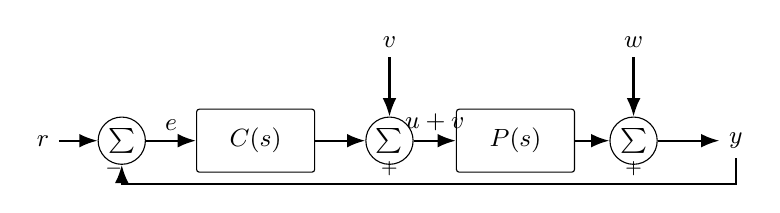
\begin{tikzpicture}[>=Latex,every node/.style={font=\small}]
			\node (r) at (-4.8,0) {$r$};
			\node[sumj] (sum) at (-3.8,0) {$\sum$};
			\node[ctlblock] (c) at (-2.1,0) {$C(s)$};
			\node[sumj] (s2) at (-0.4,0) {$\sum$};
			\node[ctlblock] (p) at (1.2,0) {$P(s)$};
			\node[sumj] (s3) at (2.7,0) {$\sum$};
			\node (y) at (4.0,0) {$y$};
			\node (v) at (-0.4,1.25) {$v$};
			\node (w) at (2.7,1.25) {$w$};
			\draw[signal] (r) -- (sum);
			\draw[signal] (sum) -- node[above] {$e$} (c);
			\draw[signal] (c) -- (s2);
			\draw[signal] (s2) -- node[above] {$u+v$} (p);
			\draw[signal] (p) -- (s3);
			\draw[signal] (s3) -- (y);
			\draw[signal] (v) -- (s2);
			\draw[signal] (w) -- (s3);
			\draw[signal] (y) -- ++(0,-0.55) -| (sum.south);
			\node[font=\scriptsize] at (-3.9,-0.35) {$-$};
			\node[font=\scriptsize] at (-0.4,-0.35) {$+$};
			\node[font=\scriptsize] at (2.7,-0.35) {$+$};
		\end{tikzpicture}
		\caption{Feedback loop with input load disturbance $v$ and additive measurement/output noise $w$.}
		\label{fig:disturbance-and-noise-loop}
	\end{figure}
	\textit{(Standard feedback loop with load disturbance $v$ at the plant input, measurement noise $w$ at the sensor output, and reference setpoint $r$).}
	The open-loop transfer function is: \[
	L(s) = P(s)C(s) \quad
	\]
	Applying superposition across all three external driving signals $(r, v, w)$ yields the fundamental algebraic relationships for error $e = r - y$, control effort $u$, and system output $y$:
	\[
	\begin{aligned} y(s) &= \left(\frac{PC}{1 + PC}\right) r + \left(\frac{P}{1 + PC}\right) v + \left(\frac{1}{1 + PC}\right) w \quad \\ e(s) &= \left(\frac{1}{1 + PC}\right) r - \left(\frac{P}{1 + PC}\right) v - \left(\frac{1}{1 + PC}\right) w \quad \\ u(s) &= \left(\frac{C}{1 + PC}\right) r - \left(\frac{PC}{1 + PC}\right) v - \left(\frac{C}{1 + PC}\right) w \quad \end{aligned}
	\]
	The \textbf{Gang of Four} represents the four central closed-loop transfer functions governing system performance and robustness:
	\begin{table}[H]
		\centering
		\small
		\begin{tabularx}{\textwidth}{>{\raggedright\arraybackslash}X>{\raggedright\arraybackslash}X}
			\toprule
			\textbf{Sensitivity function} & \textbf{Main input-output interpretation}\\
			\midrule
			$S(s)=\dfrac{1}{1+P(s)C(s)}$ & Maps reference to error and output disturbance to output; describes tracking error and feedback disturbance rejection.\\
			$T(s)=\dfrac{P(s)C(s)}{1+P(s)C(s)}$ & Maps reference to output and sensor noise to output; commonly called complementary sensitivity.\\
			$P(s)S(s)=\dfrac{P(s)}{1+P(s)C(s)}$ & Maps an input load disturbance to output; describes load-disturbance rejection.\\
			$C(s)S(s)=\dfrac{C(s)}{1+P(s)C(s)}$ & Maps sensor noise to actuator command and reference to control effort.\\
			\bottomrule
		\end{tabularx}
		\caption{The four standard closed-loop transfer functions and their roles.}
		\label{tab:gang-of-four-roles}
	\end{table}
	\textit{(The Gang of Four sensitivity transfer functions).}
	
	\subsubsection{Detailed Analysis of Each Sensitivity Function}
	\paragraph{Sensitivity Function: $S(s) = \frac{1}{1 + P(s)C(s)} = \frac{1}{1 + L(s)}$}
	\begin{itemize}
		\item
		\textbf{Tracking Error Transmission:} Relates reference $r$ to tracking error $e$: $E(s)/R(s) = S(s)$. When $|S(j\omega)| \ll 1$, tracking error is small and the system tracks commands accurately.
		\item
		\textbf{Output Disturbance Attenuation:} Relates disturbances injected at the output sensor to the measured output: $Y(s)/W(s) = S(s)$. At frequencies where $|S(j\omega)| < 1$, disturbances are actively attenuated by feedback; where $|S(j\omega)| > 1$, disturbances are amplified.
		\item
		\textbf{Robustness to Plant Variations:} Quantifies the fractional change in closed-loop transfer function $G_{cl} = T$ relative to a fractional perturbation in the physical plant model $P$: \[
		\frac{dG_{cl}}{G_{cl}} = S(s) \frac{dP}{P} \quad
		\] Small sensitivity $|S(j\omega)|$ shields closed-loop dynamics from plant parameter variations and unmodeled dynamics.
	\end{itemize}
	\paragraph{Complementary Sensitivity Function: $T(s) = \frac{P(s)C(s)}{1 + P(s)C(s)} = \frac{L(s)}{1 + L(s)}$}
	\begin{itemize}
		\item
		\textbf{Reference Tracking:} Direct closed-loop transfer function from reference $r$ to plant output $y$: $Y(s)/R(s) = T(s)$ (assuming unity feedback).
		\item
		\textbf{Sensor Noise Injection:} Relates measurement noise $w$ to output $y$. To prevent high-frequency sensor noise from corrupting system outputs, $|T(j\omega)|$ must roll off sharply at high frequencies ($|T(j\omega)| \to 0$).
		\item
		\textbf{The Complementary Identity:} Adding $S(s)$ and $T(s)$ yields the fundamental algebraic constraint: \[
		S(s) + T(s) = \frac{1}{1 + L(s)} + \frac{L(s)}{1 + L(s)} = \frac{1 + L(s)}{1 + L(s)} \equiv 1 \quad
		\] This identity proves that \textbf{$S(j\omega)$ and $T(j\omega)$ cannot be made simultaneously small at the same frequency}.
	\end{itemize}
	\paragraph{Load Disturbance Sensitivity Function: $PS(s) = \frac{P(s)}{1 + P(s)C(s)} = P(s)S(s)$}
	\begin{itemize}
		\item
		\textbf{Input Disturbance Rejection:} Governs how disturbances $v$ entering at the actuator/plant input propagate to the output $y$: $Y(s)/V(s) = PS(s)$.
		\item
		\textbf{Impact of Integral Action:} If the plant has finite DC gain ($P(0) \neq 0$) and the controller includes pure integral action ($C(s) \approx k_i/s$ as $s \to 0$), then: \[
		PS(s) = \frac{P(s)}{1 + P(s)(k_i/s)} = \frac{s P(s)}{s + k_i P(s)} \implies PS(0) = 0 \quad
		\] Integral action forces $PS(0) = 0$, guaranteeing zero steady-state error under constant step load disturbances.
	\end{itemize}
	\paragraph{Noise / Control Sensitivity Function: $CS(s) = \frac{C(s)}{1 + P(s)C(s)} = C(s)S(s)$}
	\begin{itemize}
		\item
		\textbf{Actuator Noise Transmission:} Maps high-frequency sensor noise $w$ directly into actuator control signals: $U(s)/W(s) = -CS(s)$.
		\item
		\textbf{Actuator Effort for Reference Commands:} Governs the control effort required to track references: $U(s)/R(s) = CS(s)$.
		\item
		\textbf{High-Frequency Roll-Off Requirement:} At high frequencies, physical loop gain drops ($|L(j\omega)| \to 0 \implies S(j\omega) \to 1$), reducing noise sensitivity to the controller itself: \[
		\lim_{\omega \to \infty} CS(j\omega) \approx C(j\omega) \quad
		\] If a controller uses unfiltered derivative action ($C(s) \approx K_d s$), $|C(j\omega)| \to \infty$ as $\omega \to \infty$, causing noise sensitivity to explode. This amplifies sensor noise into high-frequency actuator chatter, leading to excessive wear and actuator saturation. Practical controllers must incorporate low-pass derivative filtering to ensure $C(s)$ rolls off at high frequencies.
	\end{itemize}
	
	\subsection{Two-Degree-of-Freedom (2-DOF) Architecture \& The "Gang of Six"}
	\subsubsection{Revision Checklist}
	\begin{itemize}
		\item[$\square$]
		\textbf{Draw the block diagram} of a 2-DOF architecture incorporating a feedforward prefilter $F(s)$.
		\item[$\square$]
		\textbf{List the six transfer functions} composing the "Gang of Six".
		\item[$\square$]
		\textbf{Explain how feedforward prefilter $F(s)$ decouples} reference tracking from disturbance attenuation and robustness.
	\end{itemize}
	
	\subsubsection{Core Concepts \& Formulations}
	\paragraph{The 2-DOF Architecture}
	In a standard single-degree-of-freedom unity-feedback loop ($F(s) = 1$), the feedback compensator $C(s)$ must simultaneously manage reference tracking, load disturbance rejection, noise attenuation, and model uncertainty. Introducing a feedforward filter $F(s)$ on the reference command yields the \textbf{Two-Degree-of-Freedom (2-DOF)} structure:
	\begin{figure}[H]
		\centering
		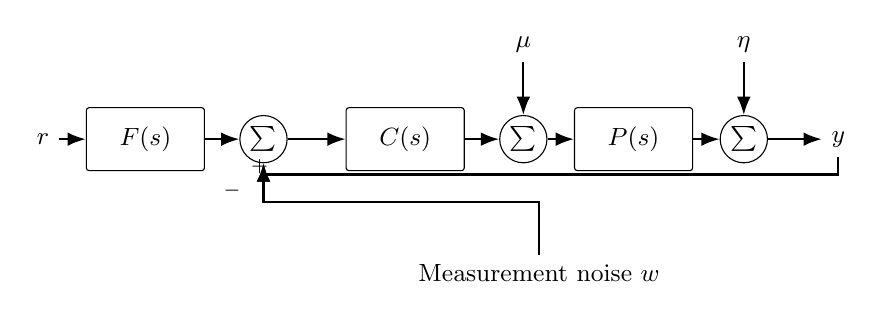
\begin{tikzpicture}[>=Latex,every node/.style={font=\small}]
			\node (r) at (-5.3,0) {$r$};
			\node[ctlblock] (f) at (-4.0,0) {$F(s)$};
			\node[sumj] (s1) at (-2.5,0) {$\sum$};
			\node[ctlblock] (c) at (-0.7,0) {$C(s)$};
			\node[sumj] (s2) at (0.8,0) {$\sum$};
			\node[ctlblock] (p) at (2.2,0) {$P(s)$};
			\node[sumj] (s3) at (3.6,0) {$\sum$};
			\node (y) at (4.8,0) {$y$};
			\node (mu) at (0.8,1.2) {$\mu$};
			\node (eta) at (3.6,1.2) {$\eta$};
			\node (w) at (1.0,-1.7) {Measurement noise $w$};
			\draw[signal] (r) -- (f);
			\draw[signal] (f) -- (s1);
			\draw[signal] (s1) -- (c);
			\draw[signal] (c) -- (s2);
			\draw[signal] (s2) -- (p);
			\draw[signal] (p) -- (s3);
			\draw[signal] (s3) -- (y);
			\draw[signal] (mu) -- (s2);
			\draw[signal] (eta) -- (s3);
			\draw[signal] (w.north) -- (1.0,-0.8) -| (s1.south);
			\draw[signal] (y) -- ++(0,-0.45) -| (s1.south);
			\node[font=\scriptsize] at (-2.55,-0.35) {$+$};
			\node[font=\scriptsize] at (-2.9,-0.65) {$-$};
		\end{tikzpicture}
		\caption{Reference prefilter, feedback controller, plant, and additive perturbations.}
		\label{fig:prefilter-disturbance-loop}
	\end{figure}
	\textit{(Two-Degree-of-Freedom feedback control architecture).}
	\paragraph{The Gang of Six Transfer Matrix}
	The complete system input-output behavior across external inputs $(r, v, w)$ is governed by the \textbf{Gang of Six}:
	\[
	\begin{bmatrix} y \\ u \end{bmatrix} = \begin{bmatrix} G_{yr}(s) & G_{yv}(s) & G_{yw}(s) \\ G_{ur}(s) & G_{uv}(s) & G_{uw}(s) \end{bmatrix} \begin{bmatrix} r \\ v \\ w \end{bmatrix} \quad
	\]
	\[
	\begin{aligned} G_{yr}(s) &= \frac{P(s)C(s)F(s)}{1 + P(s)C(s)} = F(s)T(s) \quad & G_{yv}(s) &= \frac{P(s)}{1 + P(s)C(s)} = PS(s) \quad & G_{yw}(s) &= \frac{1}{1 + P(s)C(s)} = S(s) \quad \\ G_{ur}(s) &= \frac{C(s)F(s)}{1 + P(s)C(s)} = F(s)CS(s) \quad & G_{uv}(s) &= -\frac{P(s)C(s)}{1 + P(s)C(s)} = -T(s) \quad & G_{uw}(s) &= -\frac{C(s)}{1 + P(s)C(s)} = -CS(s) \quad \end{aligned}
	\]
	\begin{itemize}
		\item
		\textbf{Design Strategy:} The feedback compensator $C(s)$ is synthesized first to optimize the \textbf{Gang of Four} ($S, T, PS, CS$), securing internal stability, robust margins, disturbance rejection, and noise filtering. The prefilter $F(s)$ is then designed independently to shape reference tracking ($G_{yr} = FT$) without degrading feedback loop robustness.
	\end{itemize}
	
	\subsection{Fundamental Design Trade-offs \& Loop Shaping}
	\subsubsection{Revision Checklist}
	\begin{itemize}
		\item[$\square$]
		\textbf{State the algebraic constraint} $S(j\omega) + T(j\omega) = 1$ and its operational consequences across frequency bands.
		\item[$\square$]
		\textbf{Define the gain crossover frequency} $\omega_{gc}$ and explain its relationship to system bandwidth.
		\item[$\square$]
		\textbf{Formulate low-frequency loop shaping objectives}: $|L(j\omega)| \gg 1$ for reference tracking and disturbance rejection.
		\item[$\square$]
		\textbf{Formulate high-frequency loop shaping objectives}: $|L(j\omega)| \ll 1$ for sensor noise attenuation and robustness.
		\item[$\square$]
		\textbf{State the crossover slope requirement} (approximately $-20\text{ dB/decade}$) to guarantee adequate phase margin.
	\end{itemize}
	
	\subsubsection{Core Concepts \& Engineering Trade-offs}
	\paragraph{The Fundamental Loop Shaping Dilemma}
	Control system design in the frequency domain involves shaping the open-loop transfer function $L(j\omega) = P(j\omega)C(j\omega)$ to manage conflicting requirements across different frequency regimes:
	\begin{lstlisting}
		Magnitude (dB)
		^
		|  Low-Frequency Band:                  High-Frequency Band:
		|  |L(jw)| >> 1                         |L(jw)| << 1
		|  S(jw) ~ 0  => Good Tracking          T(jw) ~ 0  => Noise Filtering
		|  PS(jw) ~ 0 => Disturbance Rejection  CS(jw) ~ 0 => Actuator Protection
		|  \
		|   \
		|    \  Slope near crossover ~ -20 dB/dec
		0dB+-----\----------------------------------------> Frequency w
		|      \           w_gc
		|       \
		|        \
		v         \
	\end{lstlisting}
	\textit{(Frequency-domain loop shaping objectives across operational bands).}
	\paragraph{Operational Regimes Across Frequency}
	\begin{center}\small\begin{tabularx}{\textwidth}{*{4}{Y}}
			\toprule
			\textbf{Operational Frequency Band} & \textbf{Loop Gain Requirement} & \textbf{Resulting Sensitivity Behavior} & \textbf{Engineering Objective Achieved} \\
			\midrule
			\textbf{Low Frequencies} ($\omega \ll \omega_{gc}$) & \textbf{High Loop Gain:} $\lvert L(j\omega)\rvert \gg 1$ & $S \approx 0$, $T \approx 1$, $PS \approx 0$ & Accurate reference tracking and load-disturbance rejection. \\
			\textbf{Mid Frequencies} ($\omega \approx \omega_{gc}$) & \textbf{Controlled Transition:} $\lvert L(j\omega)\rvert \approx 1$ ($0\text{ dB}$) & $\lvert S\rvert$ peaks at $M_s < 2$; loop slope near $-20\text{ dB/decade}$ & Adequate phase margin and stability margin $s_m$; well-damped closed loop. \\
			\textbf{High Frequencies} ($\omega \gg \omega_{gc}$) & \textbf{Low Loop Gain:} $\lvert L(j\omega)\rvert \ll 1$ & $S \approx 1$, $T \approx 0$, $CS$ small & Sensor-noise attenuation, actuator protection, and robustness to unmodeled dynamics. \\
			\bottomrule
	\end{tabularx}\end{center}
	\begin{itemize}
		\item
		\textbf{Bode's Gain-Phase Relationship Constraint:} To maintain closed-loop stability, the gain curve cannot drop arbitrarily steeply at crossover. A slope of $-20\text{ dB/decade}$ near $\omega_{gc}$ yields a phase lag of roughly $-90^\circ$ (leaving a healthy $+90^\circ$ phase margin). If the loop gain drops at $-40\text{ dB/decade}$ through crossover, phase lag approaches $-180^\circ$, causing phase margin to collapse to near zero and destabilizing the feedback loop.
	\end{itemize}
	
	\subsection{Internal Stability \& Hidden Instabilities (Pole-Zero Cancellations)}
	\subsubsection{Revision Checklist}
	\begin{itemize}
		\item[$\square$]
		\textbf{State the definition of internal stability} for a feedback loop in terms of all four Gang of Four transfer functions.
		\item[$\square$]
		\textbf{Explain why stability of the loop transfer function} $L(s) = P(s)C(s)$ does not guarantee closed-loop internal stability.
		\item[$\square$]
		\textbf{Analyze the hazard of RHP pole-zero cancellations} between plant and controller using the canonical counterexample.
		\item[$\square$]
		\textbf{Explain why unstable plant poles must never be cancelled} by controller zeros.
	\end{itemize}
	
	\subsubsection{Core Concepts \& Formulations}
	\paragraph{Definition of Internal Closed-Loop Stability}
	A feedback control system is \textbf{internally stable} if and only if \textbf{all four transfer functions in the Gang of Four are stable} (possess no poles in the closed right-half complex plane, $\text{Re}(s) \ge 0$). Because all four functions share the exact same characteristic denominator: \[
	D_{cl}(s) = 1 + P(s)C(s) = 1 + L(s) \quad
	\] the closed-loop system is stable under normal conditions if and only if the roots of $1 + P(s)C(s) = 0$ lie strictly in the open left-half plane.
	\paragraph{The Danger of RHP Pole-Zero Cancellations}
	Evaluating only the scalar loop transfer function $L(s) = P(s)C(s)$ or the complementary sensitivity $T(s)$ can conceal internal instability when pole-zero cancellations occur between $P(s)$ and $C(s)$ in the right-half plane.
	\paragraph{Canonical Illustrative Example}
	Consider an open-loop unstable plant controlled by a PI controller designed to cancel the unstable pole: \[
	P(s) = \frac{1}{s - a} \quad (a > 0), \quad C(s) = \frac{k(s - a)}{s} \quad
	\]
	Computing the open-loop transfer function reveals an apparent algebraic cancellation of the unstable factor $(s - a)$: \[
	L(s) = P(s)C(s) = \left(\frac{1}{s - a}\right) \left(\frac{k(s - a)}{s}\right) = \frac{k}{s} \quad
	\]
	Evaluating the sensitivity functions: \[
	S(s) = \frac{1}{1 + k/s} = \frac{s}{s + k} \quad
	\] \[
	T(s) = \frac{k/s}{1 + k/s} = \frac{k}{s + k} \quad
	\] Both $L(s)$, $S(s)$, and $T(s)$ appear stable for any $k > 0$. However, evaluating the \textbf{Load Disturbance Sensitivity} $PS(s)$ reveals the hidden instability: \[
	PS(s) = \frac{P(s)}{1 + P(s)C(s)} = \frac{\frac{1}{s - a}}{1 + \frac{k}{s}} = \frac{s}{(s - a)(s + k)} \quad
	\]
	\begin{itemize}
		\item
		\textbf{Physical Failure:} The transfer function $PS(s)$ retains the unstable open-loop pole at $s = +a$. Any non-zero load disturbance $v(t)$ at the plant input—such as a small wind gust or thermal fluctuation—excites this unobservable mode, causing the true plant output $y(t)$ to grow exponentially without bound.
		\item
		\textbf{Core Design Rule:} \textbf{Never cancel unstable plant poles with controller zeros, and never cancel unstable plant zeros with controller poles}.
	\end{itemize}
	
	\subsection{Peak Sensitivity ($M_s$), Stability Margin ($s_m$), and Robustness}
	\subsubsection{Revision Checklist}
	\begin{itemize}
		\item[$\square$]
		\textbf{Define maximum sensitivity} $M_s = \max_\omega |S(j\omega)|$ and maximum complementary sensitivity $M_t = \max_\omega |T(j\omega)|$.
		\item[$\square$]
		\textbf{Formulate the stability margin} $s_m = 1/M_s$ as the shortest Euclidean distance from the Nyquist plot to the critical point $-1$.
		\item[$\square$]
		\textbf{Explain why $s_m$ provides a more comprehensive robustness metric} than classical gain and phase margins ($g_m, \phi_m$).
		\item[$\square$]
		\textbf{State the practical engineering bounds} for $M_s$ (typically $M_s < 1.5 - 2.0$, corresponding to $s_m > 0.5$).
	\end{itemize}
	
	\subsubsection{Core Concepts \& Formulations}
	\paragraph{Peak Sensitivity ($M_s$) and the Critical Distance}
	In the complex plane, the distance from any point on the loop frequency response $L(j\omega)$ to the critical instability point $-1 + j0$ is given by $|1 + L(j\omega)|$:
	\begin{lstlisting}
		Im
		^
		|         Nyquist Curve L(jw)
		|          \
		|           \
		|            * L(jw_ms)
		|           /
		-1         |   sm     /
		--+---------+---------+---------> Re
		|  \      |        /
		|   \     |       /
		|    \----+------/
		|      |1 + L|
	\end{lstlisting}
	\textit{(Geometric relationship between the stability margin $s_m$ and the critical point $-1$).}
	From the definition of the sensitivity function: \[
	|S(j\omega)| = \frac{1}{|1 + L(j\omega)|} \quad
	\] The peak value of the sensitivity function, denoted \textbf{maximum sensitivity} $M_s$, occurs at the frequency $\omega_{ms}$ where $L(j\omega)$ makes its closest approach to $-1$: \[
	M_s = \max_{\omega} |S(j\omega)| = \frac{1}{\min_{\omega} |1 + L(j\omega)|} = \frac{1}{s_m} \quad
	\]
	where $s_m = \min_\omega |1 + L(j\omega)|$ is the \textbf{stability margin}.
	\paragraph{Why $s_m$ Beats Classical Gain and Phase Margins}
	Classical Gain Margin ($g_m$) measures distance along the negative real axis when phase lag is $-180^\circ$. Phase Margin ($\phi_m$) measures distance along the unit circle when loop gain is $0\text{ dB}$.
	\begin{itemize}
		\item
		\textbf{The Vulnerability:} Gain and phase margins evaluate perturbations independently (pure gain change \textit{or} pure phase lag). A Nyquist plot can pass dangerously close to $-1$ in the third quadrant between the axes, resulting in high gain and phase margins despite being near instability.
		\item
		\textbf{The Robustness Metric:} The stability margin $s_m$ bounds simultaneous perturbations in both gain and phase. A system designed with $M_s \le 2$ ($s_m \ge 0.5$) is guaranteed to possess: \[
		g_m \ge \frac{M_s}{M_s - 1} \ge 2 \quad (6\text{ dB}), \quad \phi_m \ge 2\arcsin\left(\frac{1}{2M_s}\right) \ge 29^\circ \quad
		\] Typically, control engineers target $M_s \in [1.3, 1.8]$ to guarantee robust stability across all operating regimes.
	\end{itemize}
	
	\subsection{Summary Comparison of the Gang of Four}
	\begin{center}\small\begin{tabularx}{\textwidth}{*{5}{Y}}
			\toprule
			\textbf{Transfer Function} & \textbf{Mathematical Definition} & \textbf{Primary Input $\to$ Output Channel} & \textbf{High Gain at Frequency $\omega$ Implies} & \textbf{Ideal Shaping Profile Across Frequency} \\
			\midrule
			\textbf{Sensitivity Function $S(s)$} & $\frac{1}{1 + P(s)C(s)}$ & Reference $r \to$ Tracking Error $e$ Output Noise $w \to$ Output $y$ & Large tracking errors, amplification of disturbances, poor robustness. & \textbf{Small at low $\omega$} ($S \approx 0$); bounded peak ($M_s < 2$) at crossover; rises to $1$ at high $\omega$. \\
			\textbf{Complementary Sensitivity $T(s)$} & $\frac{P(s)C(s)}{1 + P(s)C(s)}$ & Reference $r \to$ Output $y$ Sensor Noise $w \to$ Output $y$ & Accurate setpoint tracking ($y \approx r$), but passes sensor noise to output. & \textbf{Unity at low $\omega$} ($T \approx 1$); rolls off sharply to $0$ at high $\omega$ for noise rejection. \\
			\textbf{Load Sensitivity $PS(s)$} & $\frac{P(s)}{1 + P(s)C(s)}$ & Plant Input Disturbance $v \to$ Output $y$ & Large output deflection under external load disturbances. & \textbf{Must be forced to zero at DC} via integral action ($PS(0) = 0$); small across disturbance bandwidth. \\
			\textbf{Noise Sensitivity $CS(s)$} & $\frac{C(s)}{1 + P(s)C(s)}$ & Sensor Noise $w \to$ Control Signal $u$ Reference $r \to$ Control Effort $u$ & Dangerous high-frequency actuator chatter, wear, and saturation. & \textbf{Small at high $\omega$} achieved via controller roll-off and derivative filtering; moderate at mid-frequencies. \\
			\bottomrule
	\end{tabularx}\end{center}
	
	\subsection{MATLAB Implementation for Frequency-Domain Analysis}
	\begin{lstlisting}
		% Define Plant and Controller Transfer Functions
		s = tf('s');
		P = 1 / (s * (s + 2));              % Example 2nd-order plant
		C = 5 * (s + 1) / (s + 10);          % Lead-lag / filtered compensator
		
		% Define Open-Loop Loop Transfer Function
		L = P * C;
		
		% Construct the Gang of Four
		S  = feedback(1, L);                 % S  = 1 / (1 + L)
		T  = feedback(L, 1);                 % T  = L / (1 + L)
		PS = feedback(P, C);                 % PS = P / (1 + PC)
		CS = feedback(C, P);                 % CS = C / (1 + PC)
		
		% Generate Composite Gang of Four Bode Plots
		figure;
		subplot(2,2,1); bode(S);  grid on; title('Sensitivity S(s)');
		subplot(2,2,2); bode(T);  grid on; title('Complementary Sensitivity T(s)');
		subplot(2,2,3); bode(PS); grid on; title('Load Sensitivity PS(s)');
		subplot(2,2,4); bode(CS); grid on; title('Noise Sensitivity CS(s)');
		
		% Calculate Stability Margins & Peak Sensitivity
		[Gm, Pm, Wcg, Wcp] = margin(L);
		Ms = norm(S, Inf);                   % Peak magnitude of Sensitivity
		sm = 1 / Ms;                         % Stability Margin
		fprintf('Gain Margin: %.2f dB, Phase Margin: %.2f deg\n', 20*log10(Gm), Pm);
		fprintf('Peak Sensitivity Ms: %.2f, Stability Margin sm: %.2f\n', Ms, sm);
	\end{lstlisting}
	
	\newpage
	\section{Nyquist Stability and Robustness}
	
	\subsection{Foundations of the Nyquist Plot \& The Nyquist Contour}
	\subsubsection{Revision Checklist}
	\begin{itemize}
		\item[$\square$]
		\textbf{Define the Nyquist plot} as a polar representation of the open-loop frequency response $L(j\omega)$ over $\omega \in [-\infty, +\infty]$.
		\item[$\square$]
		\textbf{Construct the closed Nyquist D-contour ($\Gamma$)} in the complex $s$-plane enclosing the entire open right-half plane (RHP).
		\item[$\square$]
		\textbf{Apply small semicircular indentations} of radius $r \to 0$ to detour around open-loop poles on the imaginary axis.
		\item[$\square$]
		\textbf{State Cauchy’s Principle of the Argument} relating clockwise contour encirclements of the origin to zeros and poles.
		\item[$\square$]
		\textbf{Explain why the critical point is $-1 + j0$} rather than the origin when analyzing $L(s)$ instead of $1 + L(s)$.
	\end{itemize}
	
	\subsubsection{Core Concepts \& Formulations}
	\paragraph{Definition of the Nyquist Plot}
	The \textbf{Nyquist plot} of a loop transfer function $L(s) = P(s)C(s)$ is a parametric polar plot in the complex plane tracing the real and imaginary parts of $L(s)$ as the complex variable $s$ traverses a specialized closed boundary known as the \textbf{Nyquist contour}. It integrates magnitude $|L(j\omega)|$ and phase angle $\angle L(j\omega)$ into a single continuous curve, serving as the 2D polar counterpart of the dual Bode diagrams.
	\begin{lstlisting}
		Nyquist s-Plane Contour (Gamma)                     Nyquist Plot Plane L(s)
		jomega                                             Im L(s)
		^                                                ^
		+jR  |                                                |
		|  )                                             |     /---\
		|   \                                            |    /     \
		|    \                                     -1    |   |       |
		+jr  |     |  Outer Arc:                     ----+----+---+-------+---> Re L(s)
		+--\  |  s = R e^(jtheta)                        |   |    \     /
		|   | |  R -> infty, theta: +90deg -> -90deg             |    \---/
		-jr  +--/  |                                      |
		|     |                                      v
		|    /   Detour around s=0:
		|   /    s = r e^(jtheta), r -> 0
		-jR  |  )     theta: -90deg -> +90deg
		+-------------------------> sigma
	\end{lstlisting}
	\textit{(Left: The Nyquist D-contour enclosing the right-half plane. Right: Mapping into the complex loop transfer plane).}
	\paragraph{The Nyquist D-Contour ($\Gamma$)}
	To determine whether any closed-loop poles reside in the unstable right-half plane ($\text{Re}(s) > 0$), we define a closed path $\Gamma$ traversed in the \textbf{clockwise direction}:
	\begin{enumerate}
		\item
		\textbf{Positive Imaginary Axis ($C_1$):} Directed path along $s = +j\omega$ as $\omega$ ascends from $0^+$ to $+R$ (where $R \to \infty$).
		\item
		\textbf{Infinite Semicircular Arc ($C_3$):} Semicircle traversing the entire RHP given by $s = R e^{j\theta}$, with radius $R \to \infty$ and angle $\theta$ sweeping clockwise from $+90^\circ$ to $-90^\circ$.
		\item
		\textbf{Negative Imaginary Axis ($C_2$):} Directed path along $s = -j\omega$ descending from $-R$ back to $0^-$.
		\item
		\textbf{Infinitesimal Detours Around Imaginary Singularities ($C_4$):} If $L(s)$ possesses poles on the imaginary axis (e.g., pure integrators at $s = 0$ or undamped resonant poles at $\pm j\omega_0$), the contour bypasses them into the RHP along an infinitesimal semicircular arc: \[
		s = r e^{j\theta}, \quad r \to 0, \quad \theta \in [-90^\circ, +90^\circ] \text{ (clockwise)} \quad
		\]
	\end{enumerate}
	\paragraph{Cauchy’s Principle of the Argument}
	Let $F(s)$ be a single-valued, rational complex function that is analytic everywhere on and within a closed, simple clockwise contour $\Gamma$, except at a finite number of isolated poles. As $s$ traces $\Gamma$ in the clockwise direction, the mapped locus $F(\Gamma)$ encircles the origin in the complex $F$-plane $N_0$ times in the clockwise direction: \[
	N_0 = Z_F - P_F \quad
	\] where:
	\begin{itemize}
		\item
		$Z_F$ is the number of \textbf{zeros} of $F(s)$ enclosed inside contour $\Gamma$.
		\item
		$P_F$ is the number of \textbf{poles} of $F(s)$ enclosed inside contour $\Gamma$.
	\end{itemize}
	\textit{Mathematical Intuition:} Any factor $(s - z_i)$ corresponding to an enclosed zero rotates by a full net angle of $-360^\circ$ (clockwise) as $s$ completes its circuit around $\Gamma$. Any enclosed pole factor $(s - p_j)^{-1}$ contributes an opposite rotation of $+360^\circ$ (counter-clockwise). Singularities outside the contour undergo zero net angular change.
	\paragraph{Translating from Origin Encirclement to Critical Point $-1$}
	The closed-loop transfer function under negative unity feedback is: \[
	G_{cl}(s) = \frac{L(s)}{1 + L(s)} \quad
	\] Closed-loop poles are precisely the roots of the characteristic equation $1 + L(s) = 0$. Define the auxiliary function $F(s) = 1 + L(s)$:
	\begin{itemize}
		\item
		The \textbf{zeros of $F(s)$} are the roots of $1 + L(s) = 0$, which are the \textbf{closed-loop poles} of the feedback system.
		\item
		The \textbf{poles of $F(s)$} are identical to the poles of $L(s)$, which are the \textbf{open-loop poles} of the system.
	\end{itemize}
	Because $F(s) = 1 + L(s)$ is simply $L(s)$ shifted to the right by $+1$ unit in the complex plane, mapping $F(s)$ relative to the origin $0 + j0$ is identical to mapping $L(s)$ relative to the \textbf{critical point} $-1 + j0$: \[
	F(s) = 0 \iff L(s) = -1 \quad
	\]
	
	\subsection{The Nyquist Stability Criterion}
	\subsubsection{Revision Checklist}
	\begin{itemize}
		\item[$\square$]
		\textbf{State the general Nyquist stability formula} $Z = N + P$ (defining the sign convention for clockwise vs. counter-clockwise encirclements).
		\item[$\square$]
		\textbf{Define the variable meanings}: $Z$ (unstable closed-loop poles), $P$ (unstable open-loop poles), and $N$ (clockwise encirclements of $-1$).
		\item[$\square$]
		\textbf{State the condition for closed-loop stability} ($Z = 0 \iff N = -P$).
		\item[$\square$]
		\textbf{Formulate the simplified criterion} for open-loop stable systems ($P = 0 \implies N = 0$).
		\item[$\square$]
		\textbf{Analyze unstable open-loop systems} ($P > 0$) requiring active counter-clockwise encirclements to achieve stability.
	\end{itemize}
	
	\subsubsection{Core Concepts \& Formulations}
	\paragraph{The General Nyquist Stability Formula}
	Evaluating the open-loop transfer function $L(s)$ along the clockwise Nyquist contour $\Gamma$ yields the fundamental stability equation: \[
	Z = N + P \quad
	\] where:
	\begin{itemize}
		\item
		\textbf{$P \ge 0$:} The number of open-loop poles of $L(s)$ lying strictly in the open right-half plane ($\text{Re}(p) > 0$).
		\item
		\textbf{$N$:} The \textbf{net number of clockwise encirclements} of the critical point $-1 + j0$ made by the locus of $L(s)$. Counter-clockwise encirclements count as negative ($N < 0$).
		\item
		\textbf{$Z \ge 0$:} The number of closed-loop poles of the feedback system lying strictly in the open right-half plane.
	\end{itemize}
	\paragraph{Stability Condition}
	To achieve an internally stable closed-loop system, there must be \textbf{zero closed-loop poles in the right-half plane} ($Z = 0$): \[
	Z = 0 \iff N = -P \quad
	\]
	\begin{quote}
		\textbf{The General Nyquist Stability Criterion:} A feedback control system is closed-loop stable if and only if the Nyquist plot of $L(s)$ encircles the critical point $-1 + j0$ \textbf{counter-clockwise exactly $P$ times}, where $P$ is the number of open-loop right-half-plane poles of $L(s)$.
	\end{quote}
	\begin{figure}[H]
		\centering
		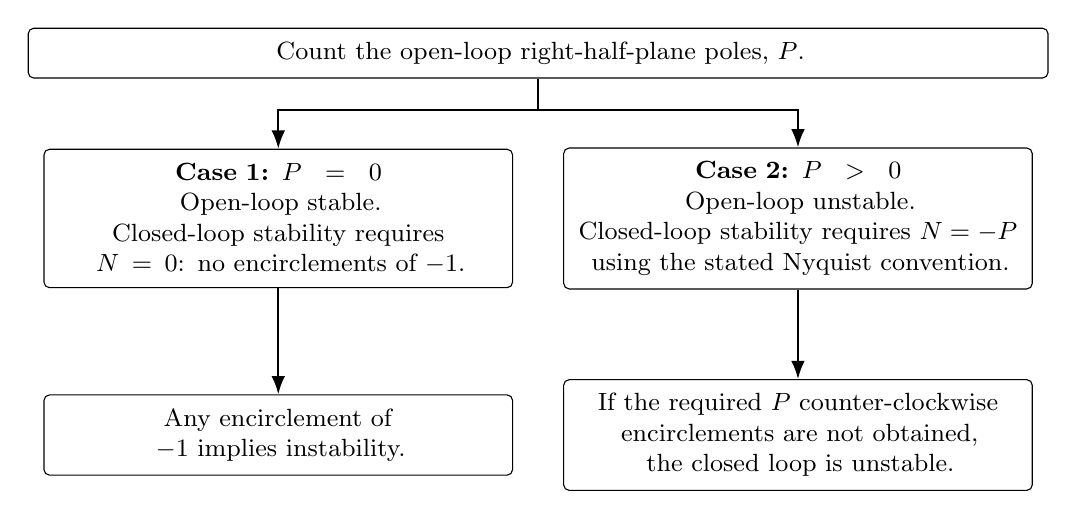
\begin{tikzpicture}[>=Latex,every node/.style={font=\small}]
			\node[flowbox] (start) at (0,3.0) {Count the open-loop right-half-plane poles, $P$.};
			\node[smallflow] (stable) at (-3.3,0.9) {\textbf{Case 1: $P=0$}\\Open-loop stable.\\Closed-loop stability requires $N=0$: no encirclements of $-1$.};
			\node[smallflow] (unstable) at (3.3,0.9) {\textbf{Case 2: $P>0$}\\Open-loop unstable.\\Closed-loop stability requires $N=-P$ using the stated Nyquist convention.};
			\node[smallflow] (bad1) at (-3.3,-1.85) {Any encirclement of $-1$ implies instability.};
			\node[smallflow] (bad2) at (3.3,-1.85) {If the required $P$ counter-clockwise encirclements are not obtained, the closed loop is unstable.};
			\draw[flowarrow] (start.south) -- ++(0,-4mm) -| (stable.north);
			\draw[flowarrow] (start.south) -- ++(0,-4mm) -| (unstable.north);
			\draw[flowarrow] (stable.south) -- (bad1.north);
			\draw[flowarrow] (unstable.south) -- (bad2.north);
		\end{tikzpicture}
		\caption{Decision guide for applying the Nyquist stability criterion after counting open-loop unstable poles.}
		\label{fig:nyquist-stability-decision}
	\end{figure}
	\textit{(Decision hierarchy for the Nyquist Stability Criterion).}
	\paragraph{The Simplified Criterion ($P = 0$)}
	When the plant and controller have no poles in the open RHP ($P = 0$), the stability condition collapses to: \[
	N = 0 \quad
	\] The closed-loop system is stable if and only if the Nyquist plot of $L(s)$ exhibits \textbf{zero net encirclements of $-1 + j0$}. Any encirclement ($N > 0$) indicates closed-loop instability ($Z = N$).
	\paragraph{Open-Loop Unstable Systems ($P > 0$)}
	When an open-loop plant is unstable ($P > 0$), stability \textbf{demands} that the Nyquist plot actively encircle the critical point $-1$ in the counter-clockwise direction.
	\begin{itemize}
		\item
		\textit{Example (Inverted Pendulum):} Consider an open-loop unstable plant $P(s) = \frac{1}{(s+1)(s-1)}$ with $P = 1$ (unstable pole at $s = +1$) stabilized by a PD compensator $C(s) = K(s+2)$. The loop transfer function is: \[
		L(s) = \frac{K(s+2)}{(s+1)(s-1)}, \quad P = 1 \quad
		\] For closed-loop stability, we require $Z = N + P = 0 \implies N = -1$ (one net counter-clockwise encirclement). Evaluating the real-axis intercept shows that for $K < 0.5$, the plot fails to encircle $-1$ ($N = 0 \implies Z = 1$, unstable). For $K > 0.5$, the locus expands to enclose $-1$ in the counter-clockwise direction ($N = -1 \implies Z = 0$), stabilizing the physical inverted pendulum.
	\end{itemize}
	
	\subsection{Systematic Nyquist Diagram Construction}
	\subsubsection{Revision Checklist}
	\begin{itemize}
		\item[$\square$]
		\textbf{Step 1:} Map the positive imaginary axis $s = +j\omega$ from $\omega = 0^+$ to $\omega \to \infty$ using polar gain and phase.
		\item[$\square$]
		\textbf{Step 2:} Map the infinite semicircle $s = R e^{j\theta}$ as $R \to \infty$; show that strictly proper transfer functions collapse to the origin.
		\item[$\square$]
		\textbf{Step 3:} Reflect the locus across the real axis to construct the negative frequency branch $s = -j\omega$.
		\item[$\square$]
		\textbf{Step 4:} Map the infinitesimal indentations around imaginary-axis poles $s = r e^{j\theta}$ as $r \to 0$ into infinite semicircular arcs.
		\item[$\square$]
		\textbf{Calculate real-axis intercept frequencies} analytically by solving $\text{Im}[L(j\omega)] = 0$.
	\end{itemize}
	
	\subsubsection{Step-by-Step Construction Procedure}
	\begin{figure}[H]
		\centering
		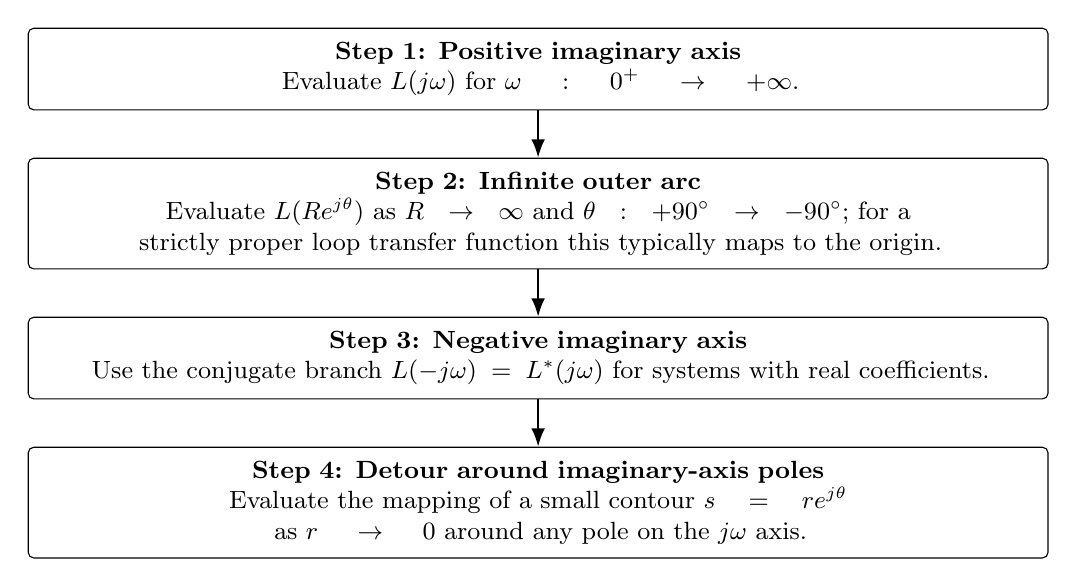
\begin{tikzpicture}[node distance=6mm,>=Latex,every node/.style={font=\small}]
			\node[flowbox] (s1) {\textbf{Step 1: Positive imaginary axis}\\Evaluate $L(j\omega)$ for $\omega:0^+\rightarrow+\infty$.};
			\node[flowbox,below=of s1] (s2) {\textbf{Step 2: Infinite outer arc}\\Evaluate $L(Re^{j\theta})$ as $R\rightarrow\infty$ and $\theta:+90^\circ\rightarrow-90^\circ$; for a strictly proper loop transfer function this typically maps to the origin.};
			\node[flowbox,below=of s2] (s3) {\textbf{Step 3: Negative imaginary axis}\\Use the conjugate branch $L(-j\omega)=L^*(j\omega)$ for systems with real coefficients.};
			\node[flowbox,below=of s3] (s4) {\textbf{Step 4: Detour around imaginary-axis poles}\\Evaluate the mapping of a small contour $s=re^{j\theta}$ as $r\rightarrow0$ around any pole on the $j\omega$ axis.};
			\draw[flowarrow] (s1) -- (s2);
			\draw[flowarrow] (s2) -- (s3);
			\draw[flowarrow] (s3) -- (s4);
		\end{tikzpicture}
		\caption{Step-by-step construction of the Nyquist contour mapping.}
		\label{fig:nyquist-construction-workflow}
	\end{figure}
	\textit{(The four-step algorithmic workflow for plotting Nyquist diagrams).}
	\paragraph{Positive Imaginary Axis ($\omega: 0^+ \to +\infty$)}
	Substitute $s = j\omega$ directly into $L(s)$: \[
	L(j\omega) = \text{Re}[L(j\omega)] + j \text{Im}[L(j\omega)] = |L(j\omega)| e^{j \angle L(j\omega)} \quad
	\] This matches the polar representation of the system’s steady-state frequency response.
	\begin{itemize}
		\item
		\textbf{Low-Frequency Anchor ($\omega \to 0^+$):} For a type-0 system, $L(j0) = K_{\text{dc}}$ on the positive real axis.
		\item
		\textbf{High-Frequency Termination ($\omega \to +\infty$):} If the relative degree $n - m \ge 1$, $|L(j\omega)| \to 0$, and the locus spirals into the origin at an asymptotic approach angle of $-(n - m) \times 90^\circ$.
	\end{itemize}
	\paragraph{Infinite Semicircular Arc ($R \to \infty$)}
	For points along $s = R e^{j\theta}$ with $\theta$ sweeping from $+90^\circ$ through $0^\circ$ to $-90^\circ$: \[
	\lim_{R \to \infty} L(R e^{j\theta}) = \lim_{R \to \infty} \frac{b_0 R^m e^{jm\theta}}{R^n e^{jn\theta}} = \lim_{R \to \infty} \frac{b_0}{R^{n-m}} e^{-j(n-m)\theta} \quad
	\] For any \textbf{strictly proper} system ($n > m$), the magnitude becomes identically zero ($0 \cdot e^{-j(n-m)\theta} = 0$), mapping the entire infinite semicircle of the $s$-plane into a single static point at the origin of the $L(s)$-plane.
	\paragraph{Negative Imaginary Axis ($\omega: -\infty \to 0^-$)}
	Because physical transfer functions have real polynomial coefficients, the frequency response satisfies Hermitian symmetry: \[
	L(-j\omega) = L^*(j\omega) = \text{Re}[L(j\omega)] - j \text{Im}[L(j\omega)] \quad
	\] The negative frequency locus is the \textbf{exact mirror image} of the positive frequency plot reflected across the horizontal real axis. The orientation arrows continue in the same continuous sequence.
	\paragraph{Handling Poles on the Imaginary Axis ($s = 0$)}
	If $L(s)$ possesses a pole at the origin of multiplicity $m$ ($L(s) = \frac{K}{s^m (Ts + 1)\dots}$), substituting the semicircular detour $s = r e^{j\theta}$ (with $r \to 0$ and $\theta$ sweeping from $-90^\circ$ to $+90^\circ$ clockwise) yields: \[
	\lim_{r \to 0} L(r e^{j\theta}) \approx \frac{K}{r^m e^{jm\theta}} = \left(\lim_{r \to 0} \frac{K}{r^m}\right) e^{-jm\theta} = \infty \cdot e^{-jm\theta} \quad
	\]
	\begin{itemize}
		\item
		\textbf{For a single integrator ($m = 1$):} As $\theta$ moves clockwise from $-90^\circ \to 0^\circ \to +90^\circ$, the phase of $L(s)$ rotates counter-clockwise from $+90^\circ \to 0^\circ \to -90^\circ$ along an arc of infinite radius in the right half of the $L(s)$-plane.
		\item
		\textbf{For a double integrator ($m = 2$):} The infinite arc sweeps through $-2 \times 180^\circ = -360^\circ$.
	\end{itemize}
	\paragraph{Analytical Determination of Real-Axis Crossings}
	To determine whether the locus encircles the critical point $-1$, find the exact crossing point on the real axis:
	\begin{enumerate}
		\item
		Separate $L(j\omega)$ into analytical real and imaginary components: \[
		L(j\omega) = u(\omega) + j v(\omega) \quad
		\]
		\item
		Set the imaginary component to zero to solve for the \textbf{phase crossover frequency} $\omega_{pc}$: \[
		v(\omega_{pc}) = \text{Im}[L(j\omega_{pc})] = 0 \quad
		\]
		\item
		Substitute $\omega_{pc}$ back into the real part to find the intercept value $L(j\omega_{pc}) = u(\omega_{pc})$. The critical gain threshold is $K_{\text{crit}} = \frac{1}{|u(\omega_{pc})|}$.
	\end{enumerate}
	
	\subsection{Stability Margins: Gain Margin, Phase Margin, and Stability Margin}
	\subsubsection{Revision Checklist}
	\begin{itemize}
		\item[$\square$]
		\textbf{Define Phase Crossover Frequency ($\omega_{pc}$)} where $\angle L(j\omega_{pc}) = -180^\circ$.
		\item[$\square$]
		\textbf{Define Gain Margin ($g_m$)} mathematically and geometrically on the Nyquist plot and Bode diagram.
		\item[$\square$]
		\textbf{Define Gain Crossover Frequency ($\omega_{gc}$)} where $|L(j\omega_{gc})| = 1$ ($0\text{ dB}$).
		\item[$\square$]
		\textbf{Define Phase Margin ($\phi_m$)} mathematically and geometrically as the angle shortfall to $-180^\circ$.
		\item[$\square$]
		\textbf{Define the Stability Margin ($s_m$)} as the minimum vector distance to $-1$: $s_m = \min_\omega |1 + L(j\omega)|$.
		\item[$\square$]
		\textbf{State the analytical lower bounds} relating $s_m$ to $g_m$ and $\phi_m$.
		\item[$\square$]
		\textbf{Explain why large $g_m$ and $\phi_m$ do not guarantee a large stability margin $s_m$}.
	\end{itemize}
	
	\subsubsection{Core Concepts \& Formulations}
	\begin{lstlisting}
		Im L(jomega)
		^
		|
		+1     |   Unit Circle (|L| = 1)
		\ | /
		\|/
		-1         -1/gm         |
		-+-----------*-----------+-------------------------> Re L(jomega)
		\         / \          |
		\  sm   /   \         |
		\     /     \        |
		\   /       * L(jomegagc)
		\ v       /
		*-------+
		L(jomegams)   \  Phase Margin: varphim = 180deg + ?L(jomegagc)
		\
	\end{lstlisting}
	\textit{(Geometric definition of Gain Margin $g_m$, Phase Margin $\phi_m$, and Stability Margin $s_m$ on the Nyquist plot).}
	\paragraph{Gain Margin ($g_m$)}
	The \textbf{Gain Margin} is the factor by which open-loop gain can be increased before the feedback system becomes unstable: \[
	\angle L(j\omega_{pc}) = -180^\circ = -\pi \text{ rad} \implies g_m = \frac{1}{|L(j\omega_{pc})|} \quad
	\] Expressed in decibels on a Bode plot: \[
	GM_{\text{dB}} = 20\log_{10}(g_m) = -20\log_{10}|L(j\omega_{pc})| \quad
	\]
	\begin{itemize}
		\item
		\textbf{Geometric Interpretation:} The Nyquist curve crosses the negative real axis at the coordinate $(-1/g_m, 0)$. Multiplying the loop by $g_m$ expands the curve radially until the intercept point touches $-1 + j0$.
	\end{itemize}
	\paragraph{Phase Margin ($\phi_m$)}
	The \textbf{Phase Margin} is the additional phase lag that can be introduced at the gain crossover frequency before the closed-loop system reaches the boundary of instability: \[
	|L(j\omega_{gc})| = 1 \quad (0\text{ dB}) \implies \phi_m = 180^\circ + \angle L(j\omega_{gc}) \quad
	\]
	\begin{itemize}
		\item
		\textbf{Geometric Interpretation:} The angle measured from the negative real axis ($-180^\circ$) to the radial line connecting the origin to the point where the Nyquist plot intersects the unit circle ($|L| = 1$).
		\item
		\textbf{Time-Delay Robustness:} A pure transport delay $e^{-s\tau}$ adds phase lag $-\omega \tau$ without altering magnitude. The maximum tolerable loop latency before instability occurs is: \[
		\tau_{\text{max}} = \frac{\phi_m}{\omega_{gc}} \quad (\phi_m \text{ in radians})
		\]
	\end{itemize}
	\paragraph{Stability Margin ($s_m$)}
	The \textbf{Stability Margin} (modulus margin) is the shortest Euclidean distance from the complete Nyquist locus $L(j\omega)$ to the critical instability point $-1 + j0$: \[
	s_m = \min_{-\infty < \omega < +\infty} |1 + L(j\omega)| \quad
	\] Geometrically, a circle centered at $-1$ with radius $s_m$ just touches the Nyquist locus without being penetrated by it.
	\paragraph{Quantitative Interrelationships}
	A large stability margin guarantees healthy gain and phase margins via the fundamental inequalities: \[
	g_m \ge \frac{1}{1 - s_m}, \quad \phi_m \ge 2 \arcsin\left(\frac{s_m}{2}\right) \quad
	\]
	\begin{itemize}
		\item
		\textit{Example Bounds:}
		\begin{itemize}
			\item
			If $s_m = 0.5 \implies g_m \ge \frac{1}{1 - 0.5} = 2 \ (6.02\text{ dB}), \quad \phi_m \ge 2\arcsin(0.25) \approx 28.96^\circ$.
			\item
			If $s_m = 0.8 \implies g_m \ge \frac{1}{1 - 0.8} = 5 \ (13.98\text{ dB}), \quad \phi_m \ge 2\arcsin(0.4) \approx 47.16^\circ$.
		\end{itemize}
	\end{itemize}
	\paragraph{Why Classical Margins Can Fail}
	Classical margins evaluate perturbations independently along specific coordinate cuts: $g_m$ checks only real-axis crossings at $-180^\circ$, while $\phi_m$ checks only the unit circle at $0\text{ dB}$.
	\begin{itemize}
		\item
		\textbf{The Vulnerability (The "Bulge" Phenomenon):} Consider a resonant plant transfer function: \[
		L(s) = \frac{0.38(s^2 + 0.1s + 0.55)}{s(s + 1)(s^2 + 0.06s + 0.5)} \quad
		\] Evaluating classical metrics yields an exceptionally large gain margin ($g_m = 266 \approx 48.5\text{ dB}$) and a healthy phase margin ($\phi_m = 70^\circ$). However, between $\omega_{gc}$ and $\omega_{pc}$, the Nyquist plot develops an internal loop that passes within $0.27$ units of the critical point ($s_m = 0.27$). A simultaneous modest gain increase combined with a minor phase lag pushes the loop around $-1$, causing unexpected closed-loop instability. \textbf{Checking $s_m$ protects against these hidden multi-variable failures}.
	\end{itemize}
	
	\subsection{Geometric and Algebraic Link to the Sensitivity Function $S(s)$}
	\subsubsection{Revision Checklist}
	\begin{itemize}
		\item[$\square$]
		\textbf{State the algebraic identity} linking the distance $|1 + L(j\omega)|$ to the Sensitivity Function $|S(j\omega)|$.
		\item[$\square$]
		\textbf{Relate the stability margin $s_m$ directly to peak sensitivity} $M_s$: $s_m = 1/M_s$.
		\item[$\square$]
		\textbf{Interpret circles centered at $-1$} in the Nyquist plane as contours of constant sensitivity magnitude.
		\item[$\square$]
		\textbf{State the standard engineering design constraint} on peak sensitivity ($M_s < 1.5 - 2.0$, ensuring $s_m > 0.5$).
	\end{itemize}
	
	\subsubsection{Core Concepts \& Formulations}
	\paragraph{Reciprocal Relationship}
	Recall the definition of the closed-loop Sensitivity Function: \[
	S(s) = \frac{1}{1 + L(s)} \implies |S(j\omega)| = \frac{1}{|1 + L(j\omega)|} \quad
	\] Because $|1 + L(j\omega)|$ is the distance from $L(j\omega)$ to $-1$, the maximum sensitivity peak $M_s$ corresponds directly to the minimum Euclidean distance $s_m$: \[
	M_s = \max_{\omega} |S(j\omega)| = \frac{1}{\min_\omega |1 + L(j\omega)|} = \frac{1}{s_m} \iff s_m = \frac{1}{M_s} \quad
	\]
	\begin{table}[H]
		\centering
		\small
		\begin{tabularx}{\textwidth}{>{\raggedright\arraybackslash}X>{\raggedright\arraybackslash}X}
			\toprule
			\textbf{Nyquist distance to $-1$} & \textbf{Sensitivity implication}\\
			\midrule
			Large distance, $s_m\gg0$ & Lower peak sensitivity (typically moderate $M_s$), moderate error amplification, greater robustness to model uncertainty, and better-damped transients.\\
			Locus approaches $-1$, $s_m\rightarrow0$ & Large sensitivity peak, strong resonant amplification, more oscillation and ringing, and fragile closed-loop stability.\\
			\bottomrule
		\end{tabularx}
		\caption{Sensitivity duality: distance from the Nyquist critical point is inversely related to peak sensitivity.}
		\label{tab:sensitivity-duality}
	\end{table}
	\textit{(Operational equivalence between geometric stability margin and sensitivity peaking).}
	\paragraph{Constant Sensitivity Contours in the Nyquist Plane}
	A circle centered at $-1 + j0$ with radius $R_c$ represents a contour of constant sensitivity magnitude: \[
	|1 + L(j\omega)| = R_c \implies |S(j\omega)| = \frac{1}{R_c} \implies |S|_{\text{dB}} = -20\log_{10}(R_c) \quad
	\]
	\begin{itemize}
		\item
		\textbf{Disturbance Attenuation Zone ($R_c > 1$):} When $L(j\omega)$ lies outside the unit circle centered at $-1$ ($|1 + L| > 1$), $|S(j\omega)| < 1$ ($< 0\text{ dB}$), and feedback attenuates disturbances.
		\item
		\textbf{Disturbance Amplification Zone ($R_c < 1$):} When $L(j\omega)$ penetrates the unit circle centered at $-1$ ($|1 + L| < 1$), $|S(j\omega)| > 1$ ($> 0\text{ dB}$), and feedback amplifies disturbances.
	\end{itemize}
	
	\subsection{Robust Stability Under Plant Uncertainty \& The Small Gain Theorem}
	\subsubsection{Revision Checklist}
	\begin{itemize}
		\item[$\square$]
		\textbf{Formulate the multiplicative uncertainty model} $P_{\text{actual}}(s) = P(s)(1 + \delta(s))$.
		\item[$\square$]
		\textbf{Derive the robust stability criterion} $|\delta(j\omega)| < \frac{1}{|T(j\omega)|}$ using Nyquist encirclement arguments.
		\item[$\square$]
		\textbf{State the Small Gain Theorem} for an interconnected feedback loop ($||H_1 \cdot H_2||_\infty < 1$).
		\item[$\square$]
		\textbf{Express the $H_\infty$ robust stability condition} $||T(s) W_m(s)||_\infty < 1$.
		\item[$\square$]
		\textbf{Explain how Complementary Sensitivity roll-off} ($T \to 0$ at high frequencies) accommodates large high-frequency modeling errors.
	\end{itemize}
	
	\subsubsection{Core Concepts \& Formulations}
	\paragraph{Modeling Plant Uncertainty}
	A nominal plant model $P(s)$ inevitably deviates from the physical process $P_{\text{actual}}(s)$ due to unmodeled high-frequency structural resonances, parameter drift, and actuator lag. Uncertainty is commonly represented as:
	\begin{enumerate}
		\item
		\textbf{Additive Uncertainty:} $P_{\text{actual}}(s) = P(s) + \Delta(s)$.
		\item
		\textbf{Multiplicative (Relative) Uncertainty:} \[
		P_{\text{actual}}(s) = P(s)\big(1 + \delta(s)\big) \quad \text{where} \quad \delta(s) = \frac{P_{\text{actual}}(s) - P(s)}{P(s)} \quad
		\] where $\Delta(s)$ and $\delta(s)$ are assumed stable, and bounded by a known frequency-dependent weighting function: $|\delta(j\omega)| \le |W_m(j\omega)|$.
	\end{enumerate}
	\begin{figure}[H]
		\centering
		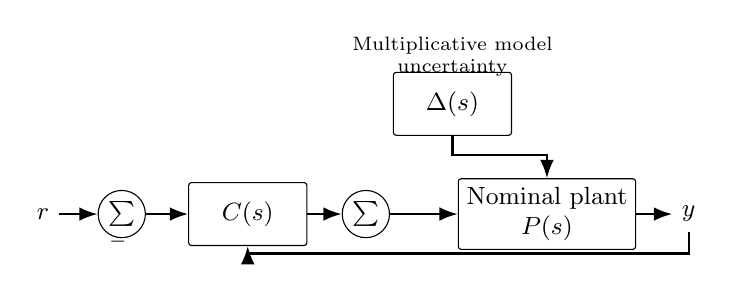
\begin{tikzpicture}[>=Latex,every node/.style={font=\small}]
			\node (r) at (-4.8,0) {$r$};
			\node[sumj] (sum) at (-3.8,0) {$\sum$};
			\node[ctlblock] (c) at (-2.2,0) {$C(s)$};
			\node[sumj] (uin) at (-0.7,0) {$\sum$};
			\node[ctlwide] (p) at (1.6,0) {Nominal plant\\$P(s)$};
			\node (y) at (3.4,0) {$y$};
			\node[ctlblock] (delta) at (0.4,1.4) {$\Delta(s)$};
			\draw[signal] (r) -- (sum);
			\draw[signal] (sum) -- (c);
			\draw[signal] (c) -- (uin);
			\draw[signal] (uin) -- (p);
			\draw[signal] (p) -- (y);
			\draw[signal] (delta.south) -- (0.4,0.75) -| (p.north);
			\draw[signal] (y) -- ++(0,-0.5) -| (c.south);
			\node[font=\scriptsize] at (-3.85,-0.35) {$-$};
			\node[align=center,font=\scriptsize] at (0.4,2.0) {Multiplicative model\\uncertainty};
		\end{tikzpicture}
		\caption{Feedback architecture with an explicit block representing multiplicative model uncertainty.}
		\label{fig:multiplicative-uncertainty-loop}
	\end{figure}
	\textit{(Feedback system with multiplicative plant uncertainty $\delta(s)$).}
	\paragraph{Derivation of the Robust Stability Condition}
	When the nominal loop $L(s) = P(s)C(s)$ is perturbed by multiplicative uncertainty, the actual loop transfer function becomes: \[
	L_{\text{actual}}(s) = P_{\text{actual}}(s)C(s) = P(s)C(s)\big(1 + \delta(s)\big) = L(s) + L(s)\delta(s) \quad
	\]
	In the complex plane, at each frequency $\omega$, the nominal point $L(j\omega)$ is surrounded by an uncertainty disk of radius $|L(j\omega)\delta(j\omega)|$. Assuming the nominal system is stable, the perturbed system remains stable if and only if the perturbed locus does not encircle or touch the critical point $-1$. Because the distance from $-1$ to the nominal point $L(j\omega)$ is $|1 + L(j\omega)|$, the uncertainty disk will not intersect $-1$ provided its radius is strictly smaller than this distance: \[
	|L(j\omega)\delta(j\omega)| < |1 + L(j\omega)|, \quad \forall \omega \ge 0 \quad
	\]
	Dividing both sides by $|L(j\omega)|$ yields: \[
	|\delta(j\omega)| < \frac{|1 + L(j\omega)|}{|L(j\omega)|} = \frac{1}{|T(j\omega)|}, \quad \forall \omega \ge 0 \quad
	\]
	\paragraph{The Small Gain Theorem Formulation}
	Isolating the uncertainty $\delta(s)$ into a standard feedback interconnection with the nominal system yields an effective transfer function looking back from the uncertainty ports of $-T(s) = -\frac{PC}{1 + PC}$. By the \textbf{Small Gain Theorem}, a closed-loop system comprising two stable interconnected operators is stable if the product of their gains is strictly less than unity: \[
	|\delta(s) \cdot T(s)|_\infty < 1 \iff |T(j\omega)| \cdot |W_m(j\omega)| < 1, \quad \forall \omega \quad
	\]
	\begin{itemize}
		\item
		\textbf{Design Implication:} At low frequencies, plant dynamics are well known ($|\delta| \ll 1$), allowing complementary sensitivity to remain near unity ($T \approx 1$) for accurate tracking. At high frequencies, where parasitic dynamics and phase shifts become large ($|\delta| \gg 1$), robust stability \textbf{demands that $T(j\omega)$ roll off rapidly to zero} ($|T(j\omega)| \ll 1/|\delta(j\omega)|$).
	\end{itemize}
	
	\subsection{Conditional Stability \& Gain Variations}
	\subsubsection{Revision Checklist}
	\begin{itemize}
		\item[$\square$]
		\textbf{Define conditional stability} for systems where stability depends on maintaining gain within an intermediate range.
		\item[$\square$]
		\textbf{Analyze real-axis multi-crossings} to determine alternating stable and unstable gain intervals.
		\item[$\square$]
		\textbf{Show how gain changes shift the effective critical point} to $-1/K$.
	\end{itemize}
	
	\subsubsection{Core Concepts \& Formulations}
	\paragraph{The Concept of Conditional Stability}
	A system is \textbf{conditionally stable} if it is stable for a nominal gain, but becomes unstable if the gain is either increased \textit{or} decreased. This occurs when the Nyquist locus crosses the negative real axis multiple times.
	\begin{itemize}
		\item
		\textit{Example:} Consider the third-order loop transfer function: \[
		L(s) = \frac{3K(s + 6)^2}{s(s + 1)^2} \quad
		\] Setting $K = 1$, the locus crosses the negative real axis twice:
		\begin{itemize}
			\item
			First crossing: $L(j\omega) = -12$ at $\omega = 2\text{ rad/s}$.
			\item
			Second crossing: $L(j\omega) = -4.5$ at $\omega = 3\text{ rad/s}$.
		\end{itemize}
	\end{itemize}
	Because $L(s)$ has no open-loop RHP poles ($P = 0$), closed-loop stability requires zero net encirclements of $-1$ ($N = 0$).
	\begin{itemize}
		\item
		For $K > \frac{2}{9} \approx 0.222$, the critical point $-1$ lies to the right of the crossings, resulting in $N = 0$ (stable).
		\item
		If gain drops into the window $\frac{1}{12} < K < \frac{2}{9}$, the critical point falls between the loops, producing two clockwise encirclements ($N = 2 \implies Z = 2$, \textbf{unstable}).
		\item
		If gain is reduced further to $K < \frac{1}{12} \approx 0.083$, the plot shrinks entirely inside the critical point, restoring $N = 0$ (stable).
		\item
		\textbf{Operational Risk:} If an actuator experiences saturation or a power amplifier suffers a supply drop, the effective loop gain falls, potentially driving a conditionally stable system from a stable operating state directly into destructive oscillation.
	\end{itemize}
	
	\subsection{Summary Comparison Table: Frequency-Domain Stability Metrics}
	\begin{center}\small\begin{tabularx}{\textwidth}{*{5}{Y}}
			\toprule
			\textbf{Robustness Metric} & \textbf{Mathematical Definition} & \textbf{Domain / Location} & \textbf{Strengths} & \textbf{Vulnerabilities / Limitations} \\
			\midrule
			\textbf{Gain Margin ($g_m$)} & $\dfrac{1}{\lvert L(j\omega_{pc})\rvert}$ & Nyquist real-axis crossing; Bode $-180^\circ$ phase line. & Simple factor by which loop gain can grow before instability. & Ignores phase; blind to near-misses between the axes. \\
			\textbf{Phase Margin ($\phi_m$)} & $180^\circ + \angle L(j\omega_{gc})$ & Nyquist unit circle crossing; Bode $0\text{ dB}$ magnitude line. & Directly correlates with damping ratio ($\zeta \approx \phi_m / 100$) and latency tolerance. & Evaluates only pure phase shift at $0\text{ dB}$; blind to mid-band resonant bulges. \\
			\textbf{Stability Margin ($s_m$)} & $\min_\omega \lvert 1 + L(j\omega)\rvert$ & Shortest vector distance from Nyquist plot to $-1$. & Bounds simultaneous gain and phase perturbations; implies lower bounds on $g_m$ and $\phi_m$. & Needs the full frequency sweep; harder to read off a Bode plot by hand. \\
			\textbf{Peak Sensitivity ($M_s$)} & $\max_\omega \lvert S(j\omega)\rvert = \dfrac{1}{s_m}$ & Peak magnitude of the sensitivity function $S(s)$. & Computed directly as $\lVert S\rVert_\infty$; one number summarizes robustness ($M_s < 2$). & Does not show where in the loop the weakness lies. \\
			\textbf{Multiplicative Uncertainty Bound} & $\lvert T(j\omega)\rvert < \dfrac{1}{\lvert\delta(j\omega)\rvert}$ & Complementary sensitivity versus the relative-error bound. & Robust-stability guarantee against unmodeled dynamics. & Conservative; needs a frequency-dependent uncertainty weight. \\
			\bottomrule
	\end{tabularx}\end{center}
	
	\subsection{Practical MATLAB Implementation}
	\begin{lstlisting}
		%% ECE4132 Week 11: Nyquist Analysis and Robust Margins Script
		clear; clc; close all;
		
		% 1. Define Open-Loop Plant and Controller
		s = tf('s');
		% Example: 3rd-order plant with potential resonance
		P = 3 / ((s + 1)^3);                 % Stable open-loop plant (P = 0)
		C = 1.5 * (s + 2) / (s + 5);         % Lead-type compensator
		L = P * C;
		
		% 2. Open-Loop Pole Count
		p_open = pole(L);
		P_rhp  = sum(real(p_open) > 0);
		fprintf('Open-Loop RHP Poles (P): %d\n', P_rhp);
		
		% 3. Plot Nyquist Diagram
		figure('Name', 'Nyquist Diagram with Stability Margin');
		nyquist(L);
		grid on; hold on;
		
		% 4. Compute Classical Gain and Phase Margins
		[Gm, Pm, Wcg, Wcp] = margin(L);
		fprintf('Gain Margin (gm): %.2f (%.2f dB) at w_pc = %.2f rad/s\n', Gm, 20*log10(Gm), Wcp);
		fprintf('Phase Margin (pm): %.2f deg at w_gc = %.2f rad/s\n', Pm, Wcg);
		
		% 5. Compute Sensitivity, Stability Margin (sm), and Peak Sensitivity (Ms)
		S = feedback(1, L);                 % S = 1 / (1 + L)
		T = feedback(L, 1);                 % T = L / (1 + L)
		
		Ms = norm(S, Inf);                  % Peak magnitude of S
		sm = 1 / Ms;                        % Shortest distance to -1
		fprintf('Peak Sensitivity (Ms): %.2f (%.2f dB)\n', Ms, 20*log10(Ms));
		fprintf('Stability Margin (sm): %.2f\n', sm);
		
		% 6. Draw Stability Margin Circle Centered at -1 on Nyquist Plot
		theta = linspace(0, 2*pi, 300);
		xc = -1 + sm * cos(theta);
		yc = sm * sin(theta);
		plot(xc, yc, 'r--', 'LineWidth', 1.5);
		plot(-1, 0, 'r+', 'MarkerSize', 10, 'LineWidth', 2);
		legend('L(s) locus', 'Stability Margin Circle (radius = s_m)', 'Critical Point (-1, 0)');
		title(sprintf('Nyquist Plot: s_m = %.2f, M_s = %.2f', sm, Ms));
		
		% 7. Robust Stability Check for Multiplicative Uncertainty
		% Assume 20% low frequency error rising to 200% at high frequency
		Wm = (2*s + 0.2) / (s + 1);         % Weighting filter bound
		figure('Name', 'Robust Stability Verification');
		bode(T, 'b', 1/Wm, 'r--');
		grid on;
		legend('|T(j\omega)|', '1 / |W_m(j\omega)| (Robustness Limit)');
		title('Robust Stability: |T| must remain strictly below 1/|W_m|');
	\end{lstlisting}
	
	\newpage
	\section{Fundamental Limitations}

	
	\subsection{Passivity in Control Systems \& Frequency-Domain Implications}
	\subsubsection{Revision Checklist}
	\begin{itemize}
		\item[$\square$]
		\textbf{Define passivity} from an energy-conservation and dissipation perspective.
		\item[$\square$]
		\textbf{Identify physical examples} of passive physical plants (e.g., $RC$ filters, mass-spring-damper systems with friction).
		\item[$\square$]
		\textbf{State the Nyquist plane condition} for a passive open-loop transfer function ($\text{Re}[L(j\omega)] \ge 0$).
		\item[$\square$]
		\textbf{Prove geometrically and algebraically} why passivity guarantees $|S(j\omega)| \le 1$ (and $M_s \le 1$) for all frequencies.
		\item[$\square$]
		\textbf{Explain why passive loops completely avoid} the "waterbed effect" and high-sensitivity peaking ($M_s > 1$).
	\end{itemize}
	
	\subsubsection{Core Concepts \& Formulations}
	\paragraph{Physical Definition of Passivity}
	A dynamical system is \textbf{passive} if it cannot produce net internal energy. It can only store or dissipate energy supplied by external sources.
	\begin{itemize}
		\item
		\textbf{Physical Examples:} Passive electrical networks containing only resistors, inductors, and capacitors ($RLC$), fluidic flow dampers, and mechanical networks containing mass, stiffness, and friction.
		\item
		\textbf{Positive Real Property:} The transfer function $L(s)$ of a linear time-invariant passive system is \textit{positive real}, satisfying: \[
		\text{Re}[L(s)] \ge 0 \quad \text{for all } s \text{ with } \text{Re}(s) \ge 0
		\]
	\end{itemize}
	\paragraph{Frequency-Domain and Nyquist Interpretation}
	For any passive open-loop loop transfer function $L(s)$, the frequency response curve $L(j\omega)$ is strictly confined to the \textbf{closed right-half of the complex plane} for all frequencies $\omega \in (-\infty, +\infty)$: \[
	\text{Re}[L(j\omega)] \ge 0, \quad \forall \omega \in \mathbb{R} \quad
	\]
	\begin{lstlisting}
		Im L(jomega)
		^
		|       Passive Region:
		|       Re[L(jomega)] >= 0
		|
		|          * L(jomega)
		-1               |         /
		-+---------------+--------+----------> Re L(jomega)
		|               |       /
		|               |      /
		|<--- |1+L| --->|     /
		|               |    /
		|               |   v
		|               |  Nyquist locus stays
		|               |  entirely in the RHP!
	\end{lstlisting}
	\textit{(Geometric proof: For any passive loop $L(j\omega)$ residing in the right-half plane, the distance to the critical point $-1$ is always $|1 + L(j\omega)| \ge 1$).}
	\paragraph{Why Passivity Guarantees $|S(j\omega)| \le 1$ Everywhere}
	Recall the definition of the Sensitivity Function: \[
	S(s) = \frac{1}{1 + L(s)} \implies |S(j\omega)| = \frac{1}{|1 + L(j\omega)|} \quad
	\] In the complex plane, the denominator $|1 + L(j\omega)|$ is the Euclidean distance from the critical instability point $-1 + j0$ to the point $L(j\omega)$ on the Nyquist curve.
	\begin{enumerate}
		\item
		Because $L(j\omega)$ is constrained to the right-half plane ($\text{Re}[L(j\omega)] \ge 0$), the real part of $1 + L(j\omega)$ satisfies: \[
		\text{Re}[1 + L(j\omega)] = 1 + \text{Re}[L(j\omega)] \ge 1 \quad
		\]
		\item
		Computing the magnitude: \[
		|1 + L(j\omega)| = \sqrt{\big(1 + \text{Re}[L(j\omega)]\big)^2 + \big(\text{Im}[L(j\omega)]\big)^2} \ge \sqrt{1^2 + 0} = 1 \quad
		\]
		\item
		Taking the reciprocal directly yields: \[
		|S(j\omega)| = \frac{1}{|1 + L(j\omega)|} \le 1, \quad \forall \omega \in \mathbb{R} \quad
		\]
		\item
		Consequently, the \textbf{peak sensitivity} satisfies: \[
		M_s = \max_{\omega} |S(j\omega)| \le 1 \quad
		\]
	\end{enumerate}
	\begin{itemize}
		\item
		\textbf{Design Consequence:} In a strictly passive feedback loop, feedback \textbf{never amplifies external disturbances or errors at any frequency} ($|S(j\omega)| \le 1$ everywhere). The loop possesses infinite gain margin, at least $90^\circ$ of phase margin, and does not experience resonant peaking. It represents the rare case where feedback operates without triggering the trade-offs described by the waterbed effect.
	\end{itemize}
	
	\subsection{Peak Sensitivity $M_s$ and Stability Margin Geometry}
	\subsubsection{Revision Checklist}
	\begin{itemize}
		\item[$\square$]
		\textbf{Relate peak sensitivity} $M_s = \max_\omega |S(j\omega)|$ to the stability margin $s_m = \min_\omega |1 + L(j\omega)|$ ($M_s = 1/s_m$).
		\item[$\square$]
		\textbf{Explain why $M_s \ge 1$} for any non-trivial, non-passive feedback system.
		\item[$\square$]
		\textbf{Identify the peak frequency} $\omega_{ms}$ and explain why closed-loop disturbance amplification is worst at $\omega_{ms}$.
		\item[$\square$]
		\textbf{State the practical target ranges} for $M_s$ ($1.3 \le M_s \le 2.0$, or $3\text{ dB}$ to $6\text{ dB}$).
	\end{itemize}
	
	\subsubsection{Core Concepts \& Formulations}
	\paragraph{Peak Sensitivity as a Robustness Indicator}
	For general physical plants (which are non-passive due to actuators, sensors, computing delays, or right-half-plane singularities), the loop locus $L(j\omega)$ enters the left-half plane, passing near $-1$.
	\begin{itemize}
		\item
		\textbf{Maximum Sensitivity ($M_s$):} \[
		M_s = \max_{-\infty < \omega < +\infty} |S(j\omega)| = \frac{1}{\min_\omega |1 + L(j\omega)|} = \frac{1}{s_m} \quad
		\] where $s_m$ is the shortest vector distance from the Nyquist plot to $-1$.
		\item
		\textbf{Physical Significance of $M_s$:}
		\begin{itemize}
			\item
			If $M_s \approx 1$ ($0\text{ dB}$), the closed-loop system never amplifies disturbances by more than unity.
			\item
			If $M_s \gg 2$ (e.g., $M_s = 5 \implies 14\text{ dB}$), the system amplifies measurement noise and load disturbances by a factor of 5 near the frequency $\omega_{ms}$, exhibiting low damping, large step overshoot, and high vulnerability to parameter uncertainty.
			\item
			Control engineers target $M_s \in [1.3, 1.8]$ ($2.3\text{ dB}$ to $5.1\text{ dB}$) to ensure acceptable stability margins ($s_m \ge 0.55$).
		\end{itemize}
	\end{itemize}
	\begin{lstlisting}
		Log Magnitude |S(jomega)|
		^
		|                        Peak Sensitivity Ms = max |S(jomega)|
		|                                   * (At frequency omega_ms)
		|                                  / \
		1.0 +---------------------------------+---+-------------------- Line |S| = 1 (0 dB)
		|   Error Attenuation Band       /     \     Unattenuated Region
		|   |S(jomega)| < 1                 /       \    |S(jomega)| ~ 1
		|   (Tracking & Regulation)    /         \
		0.0 +-----------------------------+           +----------------> Frequency omega
		0                            omega_sc
	\end{lstlisting}
	\textit{(Typical sensitivity frequency response showing the low-frequency attenuation band, crossover at $\omega_{sc}$, and the resonant sensitivity peak $M_s$).}
	
	\subsection{Bode's Integral Formula \& The "Waterbed Effect" (Stable Systems)}
	\subsubsection{Revision Checklist}
	\begin{itemize}
		\item[$\square$]
		\textbf{State the roll-off assumption} required for Bode's integral formula ($\lim_{s \to \infty} s L(s) = 0$, relative degree $\ge 2$).
		\item[$\square$]
		\textbf{State Bode's Integral Formula} for an open-loop stable loop transfer function: \[
		\int_{0}^{\infty} \ln |S(j\omega)|\, d\omega = 0 \quad
		\]
		\item[$\square$]
		\textbf{Explain the geometric meaning} of positive area ($\ln |S| > 0$) versus negative area ($\ln |S| < 0$).
		\item[$\square$]
		\textbf{State the physical meaning} of the "waterbed effect" (conservation of sensitivity volume).
		\item[$\square$]
		\textbf{Explain why pushing sensitivity down} at low frequencies forces sensitivity to pop up above unity elsewhere.
	\end{itemize}
	
	\subsubsection{Core Concepts \& Formulations}
	\paragraph{Theorem: Bode's Integral Formula for Stable Systems}
	Let $S(s) = \frac{1}{1 + L(s)}$ be the sensitivity function of an internally stable feedback system. If the open-loop transfer function $L(s) = P(s)C(s)$ has a relative degree of at least 2 (such that $\lim_{s \to \infty} s L(s) = 0$), and has \textbf{no poles in the closed right-half complex plane} (open-loop stable), then:
	\[
	\int_{0}^{\infty} \ln |S(j\omega)|\, d\omega = \int_{0}^{\infty} \ln \frac{1}{|1 + L(j\omega)|}\, d\omega = 0 \quad
	\]
	\textit{(Note: The integration is taken with respect to frequency $\omega$ on a \textbf{linear scale}, while sensitivity magnitude is evaluated on a natural logarithmic scale).}
	\paragraph{Geometric and Physical Interpretation}
	Because $\ln(1) = 0$:
	\begin{itemize}
		\item
		When $|S(j\omega)| < 1$, $\ln |S(j\omega)| < 0$ (yielding a \textbf{negative area} below the zero line where disturbances are attenuated).
		\item
		When $|S(j\omega)| > 1$, $\ln |S(j\omega)| > 0$ (yielding a \textbf{positive area} above the zero line where disturbances are amplified).
	\end{itemize}
	Bode's theorem states that the total net area is conserved identically at zero: \[
	\text{Area Below Zero Line } (\ln |S| < 0) = \text{Area Above Zero Line } (\ln |S| > 0) \quad
	\]
	\begin{lstlisting}
		ln|S(jomega)|
		^
		|                               Area Above (ln|S| > 0):
		|                               Disturbance Amplification (|S| > 1)
		|                                    +--------+
		|                                   / :::::::  \
		0 --+----------------------------------+------------+-----------------> Frequency omega
		| \  ::::::::::::::::: /           omega_sc          \
		|  \  Negative Area   /                           \
		|   +----------------+                             +---> Asymptotic 0 dB
		|   Area Below (ln|S| < 0):
		|   Disturbance Attenuation (|S| < 1)
		v
		Net Area Below = Net Area Above  (Total Integral = 0)
	\end{lstlisting}
	\textit{(Graphical representation of Bode's Integral: The area of attenuation below zero must be balanced by an equal area of amplification above zero).}
	\paragraph{The "Waterbed Effect"}
	Bode's integral acts as a fundamental law of conservation in feedback systems:
	\begin{itemize}
		\item
		\textbf{The Analogy:} Pushing down on one part of a waterbed causes another part to bulge upward.
		\item
		\textbf{The Engineering Compromise:} If an engineer increases controller gains to force $|S(j\omega)| \ll 1$ across a wider tracking bandwidth $[0, \omega_1]$, the negative area increases. To maintain the zero integral sum, \textbf{$|S(j\omega)|$ must exceed unity across an adjacent frequency band}, producing a sensitivity peak ($M_s > 1$).
		\item
		\textbf{Stein’s Dirt-Mound Analogy:} Gunter Stein compared control design to shoveling dirt on an uneven mound: you cannot remove the volume of dirt; you can only shovel it from one frequency range into another. A skilled designer moves the inevitable amplification peak into a benign frequency band where disturbance power and measurement noise are minimal.
	\end{itemize}
	
	\subsection{Unstable Plants: The Generalized Bode Integral}
	\subsubsection{Revision Checklist}
	\begin{itemize}
		\item[$\square$]
		\textbf{State the generalized Bode Integral Formula} for plants with open-loop right-half-plane poles $p_k$: \[
		\int_{0}^{\infty} \ln |S(j\omega)|\, d\omega = \pi \sum_{p_k > 0} p_k \quad
		\]
		\item[$\square$]
		\textbf{Explain why the presence of RHP poles makes the waterbed effect strictly worse}.
		\item[$\square$]
		\textbf{State the exponential lower bound on peak sensitivity} $M_s$ when controlling an unstable plant over a finite bandwidth.
		\item[$\square$]
		\textbf{Explain why multiple or fast unstable poles} force high sensitivity and severe closed-loop fragility.
	\end{itemize}
	
	\subsubsection{Core Concepts \& Formulations}
	\paragraph{Theorem: Generalized Bode Integral for Unstable Systems}
	Assume the closed-loop system is internally stabilized by feedback controller $C(s)$, with relative degree $\ge 2$. If the open-loop transfer function $L(s) = P(s)C(s)$ has $m$ unstable poles $p_1, p_2, \dots, p_m$ in the open right-half complex plane ($\text{Re}(p_k) > 0$), then:
	\[
	\int_{0}^{\infty} \ln |S(j\omega)|\, d\omega = \pi \sum_{k=1}^{m} \text{Re}(p_k) \quad
	\]
	\textit{(If an unstable pole is a complex conjugate pair $p$, $p_{i,j} = \sigma \pm j\omega_0$, their combined contribution to the right-hand sum is $\pi(\sigma + \sigma) = 2\pi\sigma$).}
	\paragraph{Physical Meaning: The Price of Unstable Dynamics}
	Because the real parts of open-loop RHP poles are strictly positive ($\text{Re}(p_k) > 0$), the right-hand side of Bode's formula is \textbf{strictly positive}: \[
	\int_{0}^{\infty} \ln |S(j\omega)|\, d\omega = \pi \sum_{k=1}^m p_k > 0 \quad
	\]
	This leads to two consequences:
	\begin{enumerate}
		\item
		\textbf{Positive Area Dominance:} The positive area (where $|S| > 1$, error amplification) must exceed the negative area (where $|S| < 1$, error suppression) by an amount equal to $\pi \sum p_k$.
		\item
		\textbf{The Penalty of Instability:} The feedback controller must "pay" for stabilizing an open-loop unstable mode by accepting larger sensitivity and degraded robustness in other frequency bands. Fast unstable poles (large positive $p_k$) impose a severe penalty, making tight disturbance rejection difficult to achieve.
	\end{enumerate}
	\paragraph{Exponential Bound on Peak Sensitivity}
	Consider an open-loop plant with an unstable pole at $s = +p$ ($p > 0$). Suppose the designer requires good disturbance attenuation ($|S(j\omega)| \le \epsilon < 1$) over the operational bandwidth $\omega \in [0, \omega_1]$, and measurement noise prevents active feedback beyond the actuator bandwidth $\omega_a$ (such that $|S(j\omega)| \approx 1$ for $\omega \ge \omega_a$):
	\begin{lstlisting}
		|S(jomega)|
		^
		Ms +                         +---------------------+
		|                        /|                     |
		|                       / |                     |
		|                      /  |                     |
		1.0 +                     /   |                     +------- |S| = 1
		|                    /    |
		|                   /     |
		varepsilon +------------------+      |
		0                 omega1     omegaa                             Frequency omega
		Low-Sensitivity       Actuator Cutoff
	\end{lstlisting}
	\textit{(Piecewise sensitivity model illustrating the exponential lower bound on $M_s$).}
	Evaluating Bode's integral under this piecewise profile yields the lower bound on peak sensitivity: \[
	M_s \ge \exp\left( \frac{\pi p + \omega_1(1 - \epsilon)}{\omega_a - \omega_1} \right) \quad
	\]
	\begin{itemize}
		\item
		\textbf{Exponential Sensitivity Growth:} As the target tracking bandwidth $\omega_1$ approaches the actuator bandwidth limit $\omega_a$, the denominator $(\omega_a - \omega_1) \to 0$, causing $M_s \to \infty$ exponentially.
		\item
		\textbf{Minimum Actuator Bandwidth Requirement:} To maintain peak sensitivity within acceptable bounds ($M_s \le 2 \implies \ln M_s \approx 0.693$), the actuator bandwidth $\omega_a$ must be significantly larger than the open-loop unstable pole location: \[
		\omega_a \gg \pi p + \omega_1
		\] If actuator bandwidth is insufficient, \textbf{stabilization is impossible without severe closed-loop resonant peaking and fragility}.
	\end{itemize}
	
	\subsection{Mathematical Proof of Bode's Integral Formula}
	\subsubsection{Revision Checklist}
	\begin{itemize}
		\item[$\square$]
		\textbf{Construct the closed integration contour} $\Gamma$ enclosing the entire RHP and indenting around open-loop unstable poles $p_k$.
		\item[$\square$]
		\textbf{Apply Cauchy’s Residue Theorem} to the analytic complex logarithm $\ln S(s)$ along $\Gamma$.
		\item[$\square$]
		\textbf{Evaluate the contour integral along the imaginary axis}: \[
		I_1 = -2j \int_{0}^{\infty} \ln |S(j\omega)|\, d\omega \quad
		\]
		\item[$\square$]
		\textbf{Evaluate the semicircular indentations} around each open-loop pole $p_k$ to extract the residues $-2\pi j p_k$.
		\item[$\square$]
		\textbf{Show that the integral along the infinite outer arc vanishes} when $\lim_{s \to \infty} s L(s) = 0$.
	\end{itemize}
	
	\subsubsection{Step-by-Step Mathematical Derivation}
	\paragraph{Integration Contour Setup}
	Consider the sensitivity function $S(s) = \frac{1}{1 + L(s)}$. Since the closed-loop system is internally stable, $1 + L(s)$ has no zeros in the closed right-half plane ($\text{Re}(s) \ge 0$), meaning $S(s)$ has no poles in the RHP. However, whenever the open-loop transfer function $L(s)$ has a pole at $s = p_k$ with $\text{Re}(p_k) > 0$, $L(p_k) \to \infty$, which causes the sensitivity function to vanish: \[
	S(p_k) = \frac{1}{1 + L(p_k)} = 0 \implies \ln S(p_k) \to -\infty \quad
	\]
	Thus, the function $f(s) = \ln S(s)$ has isolated logarithmic branch points at every open-loop RHP pole $p_k$. To apply Cauchy's theorem, construct a counter-clockwise contour $\Gamma$ in the complex $s$-plane consisting of:
	\begin{enumerate}
		\item
		The imaginary axis from $s = -jR$ to $s = +jR$.
		\item
		The infinite outer semicircular arc $s = R e^{j\theta}$ for $\theta \in [-\pi/2, +\pi/2]$ with $R \to \infty$.
		\item
		Lateral cuts connecting the imaginary axis to small circles of radius $\epsilon \to 0$ enclosing each RHP pole $p_k$.
	\end{enumerate}
	\begin{lstlisting}
		Contour Gamma for Proving Bode's Integral Formula
		jomega
		^
		+jR |       Outer Arc: s = R e^(jtheta)
		|    )  R -> infty, theta: +90deg -> -90deg
		|     \
		|      \
		+----->--* pk (Open-loop pole detour)
		|<----- /
		|      /
		|     /
		-jR |    )
		+-------------------------> sigma
	\end{lstlisting}
	\textit{(Contour $\Gamma$ enclosing the right-half plane while detouring around isolated singularities at $s = p_k$).}
	\paragraph{Cauchy’s Integral Application}
	Because $f(s) = \ln S(s)$ is analytic everywhere inside and on $\Gamma$, Cauchy's Integral Theorem gives: \[
	\oint_{\Gamma} \ln S(s)\, ds = 0 \quad
	\]
	Splitting the closed contour integral into its constituent geometric segments: \[
	\int_{\text{Imaginary Axis}} \ln S(s)\, ds + \int_{\text{Outer Arc}} \ln S(s)\, ds + \sum_{k=1}^m \oint_{\text{Detour}(p_k)} \ln S(s)\, ds = 0 \quad
	\]
	\paragraph{Imaginary Axis Segment ($s = j\omega$)}
	Along the imaginary axis, $s = j\omega$ and $ds = j\, d\omega$: \[
	\int_{-j\infty}^{+j\infty} \ln S(s)\, ds = j \int_{-\infty}^{+\infty} \ln S(j\omega)\, d\omega = j \int_{-\infty}^{+\infty} \big( \ln |S(j\omega)| + j \angle S(j\omega) \big)\, d\omega \quad
	\] Because the magnitude $|S(j\omega)|$ is an even function of $\omega$ ($\ln |S(-j\omega)| = \ln |S(j\omega)|$) and the phase angle $\angle S(j\omega)$ is an odd function ($\angle S(-j\omega) = -\angle S(j\omega)$), the imaginary part integrates to zero, leaving: \[
	\int_{-j\infty}^{+j\infty} \ln S(s)\, ds = 2j \int_{0}^{\infty} \ln |S(j\omega)|\, d\omega \quad
	\]
	\paragraph{Infinite Semicircular Outer Arc ($R \to \infty$)}
	Along the outer arc, $s = R e^{j\theta}$ with $\theta \in [\pi/2, -\pi/2]$. Since relative degree $\ge 2$, $L(s) \approx \frac{K}{s^k}$ ($k \ge 2$) for large $s$, so $\lim_{s \to \infty} s L(s) = 0$. Using the Taylor series approximation $\ln(1 + x) \approx x$ for small $x$: \[
	\ln S(s) = \ln \frac{1}{1 + L(s)} = -\ln(1 + L(s)) \approx -L(s)
	\] Evaluating along the outer semicircle: \[
	\left| \int_{\text{Outer Arc}} \ln S(s)\, ds \right| \le \int_{-\pi/2}^{\pi/2} |L(R e^{j\theta})| R\, d\theta \to 0 \quad \text{as } R \to \infty \quad
	\]
	\paragraph{Evaluation of Singular Pole Detours}
	For each isolated pole $p_k$, the forward and return paths along the lateral cut cancel out. Integrating counter-clockwise around the small circular contour enclosing $p_k$ via integration by parts yields: \[
	\oint \ln S(s)\, ds = -2\pi j , p_k \quad
	\]
	\paragraph{Assembling the Terms}
	Substituting all evaluated segments into Cauchy’s equation: \[
	2j \int_{0}^{\infty} \ln |S(j\omega)|\, d\omega - 2\pi j \sum_{k=1}^m p_k = 0
	\] Dividing through by $2j$ yields Bode’s Integral Formula: \[
	\int_{0}^{\infty} \ln |S(j\omega)|\, d\omega = \pi \sum_{k=1}^m p_k \quad
	\]
	
	\subsection{Fundamental Limits Imposed by RHP Zeros, Delays, and RHP Poles}
	\subsubsection{Revision Checklist}
	\begin{itemize}
		\item[$\square$]
		\textbf{Explain why Right-Half-Plane (RHP) zeros} cannot be cancelled by a stabilizing controller.
		\item[$\square$]
		\textbf{State the Complementary Sensitivity integral formula} for open-loop RHP zeros $z_k$: \[
		\int_{0}^{\infty} \frac{\ln |T(j\omega)|}{\omega^2}\, d\omega = \pi \sum_{z_k > 0} \frac{1}{z_k} \quad
		\]
		\item[$\square$]
		\textbf{Apply the Maximum Modulus Principle} to establish interpolation constraints: $S(z) = 1$ and $T(p) = 1$.
		\item[$\square$]
		\textbf{Derive the sensitivity peak bound} for a plant with both an RHP pole $p$ and an RHP zero $z$: \[
		M_s \ge \left| \frac{z + p}{z - p} \right| \quad
		\]
		\item[$\square$]
		\textbf{Formulate crossover frequency bounds} imposed by non-minimum-phase zeros ($\omega_{sc} < z$) and time delays ($\omega_{gc} \tau \le \phi_{ap}$).
	\end{itemize}
	
	\subsubsection{Core Concepts \& Formulations}
	\paragraph{Right-Half-Plane (RHP) Zeros and Complementary Sensitivity}
	A zero in the right-half plane ($s = +z_0,\; z_0 > 0$) introduces phase lag without altering magnitude, making the system \textbf{non-minimum-phase}.
	\begin{itemize}
		\item
		\textbf{Bode’s Integral for Complementary Sensitivity:} An integral formula dual to Bode's sensitivity integral applies to $T(s)$: \[
		\int_{0}^{\infty} \frac{\ln |T(j\omega)|}{\omega^2}\, d\omega = \pi \sum_{k=1}^{\ell} \frac{1}{z_k} \quad
		\] where $z_k$ are the RHP zeros of the open-loop transfer function.
		\item
		\textbf{Physical Implication:} Slow RHP zeros (small $z_k$) yield large values of $1/z_k$, creating a large positive area under $\ln |T|/\omega^2$. Because accurate command tracking requires $T \approx 1$ ($\ln |T| \approx 0$) at low frequencies, \textbf{slow RHP zeros force significant peak overshoot or amplification in complementary sensitivity ($M_t > 1$)}.
	\end{itemize}
	\paragraph{Maximum Modulus Principle \& Interpolation Constraints}
	For an internally stable feedback loop, the closed-loop transfer functions must satisfy the following algebraic interpolation conditions:
	\begin{enumerate}
		\item
		\textbf{At an open-loop RHP zero $z$ ($P(z) = 0 \implies L(z) = 0$):} \[
		S(z) = \frac{1}{1 + L(z)} = 1, \quad T(z) = \frac{L(z)}{1 + L(z)} = 0
		\]
		\item
		\textbf{At an open-loop RHP pole $p$ ($P(p) \to \infty \implies L(p) \to \infty$):} \[
		S(p) = 0, \quad T(p) = 1
		\]
	\end{enumerate}
	By the \textbf{Maximum Modulus Principle}, the maximum of an analytic function in the right-half plane must occur on its boundary (the imaginary axis $j\omega$). Therefore: \[
	M_s = \max_{\omega} |S(j\omega)| \ge |S(z)| = 1, \quad M_t = \max_{\omega} |T(j\omega)| \ge |T(p)| = 1 \quad
	\]
	\paragraph{Combined RHP Pole and Zero Interaction}
	If a physical plant possesses \textbf{both an unstable pole $p$ and a non-minimum-phase zero $z$} in the right-half plane, the all-pass factor relating them produces a strict bound on peak sensitivity:
	\[
	M_s \ge \left| \frac{z + p}{z - p} \right|, \quad M_t \ge \left| \frac{z + p}{z - p} \right| \quad
	\]
	\begin{lstlisting}
		Sensitivity Peak Lower Bound Ms
		^
		|      |z + p|
		| Ms >= -------
		|      |z - p|
		|
		|                     As p -> z, Ms -> infty!
		|                     Severe Control Limitation!
		|                         |
		|                        /
		1.0 +-----------------------+--------------------> Ratio p / z
		0                       1
	\end{lstlisting}
	\textit{(Sensitivity peaking as an RHP pole $p$ approaches an RHP zero $z$).}
	\begin{itemize}
		\item
		\textbf{The Pole-Zero Proximity Disaster:} If an unstable pole is located close to a non-minimum-phase zero ($p \approx z$), the denominator $|z - p| \to 0$, forcing \textbf{$M_s \to \infty$ and stability margin $s_m \to 0$}. Such plants are virtually impossible to control robustly.
	\end{itemize}
	\paragraph{Bandwidth and Crossover Limits Summary}
	\begin{center}\small\begin{tabularx}{\textwidth}{*{4}{Y}}
			\toprule
			\textbf{Plant Limitation} & \textbf{Underlying Mechanism} & \textbf{Strict Frequency-Domain Constraint} & \textbf{Practical Design Rule} \\
			\midrule
			\textbf{Real RHP Zero ($z$)} & Inherent phase lag; initial undershoot in time response. & $\omega_{sc} \le z \sqrt{\frac{M_s - 1}{M_s + 1}}$ & Keep bandwidth well below the zero: $\omega_{gc} < 0.5 z$. \\
			\textbf{Pure Time Delay ($\tau$)} & Linear phase drop $\angle(e^{-j\omega\tau}) = -\omega\tau$ with no gain attenuation. & $\omega_{gc} \tau \le \phi_{ap} \quad (\phi_{ap} \approx 45^\circ - 60^\circ)$ & Limit crossover frequency: $\omega_{gc} < \frac{1}{\tau}$. \\
			\textbf{Real RHP Pole ($p$)} & Inherent dynamic divergence requiring fast stabilizing action. & $\omega_{tc} \ge p \sqrt{\frac{M_t + 1}{M_t - 1}}$ & Bandwidth must exceed the pole: $\omega_{gc} > 2 p$. \\
			\textbf{Combined RHP Pole \& Zero ($p, z$)} & Conflicting bandwidth requirements: $\omega_{gc}$ must be $> 2p$ and $< 0.5z$. & $M_s \ge \left\lvert \dfrac{z + p}{z - p} \right\rvert$ & Avoid designs with $p \approx z$; $M_s \to \infty$ as the pole approaches the zero. \\
			\bottomrule
	\end{tabularx}\end{center}
	
	\subsection{Gunter Stein’s "Respect the Unstable" \& The X-29 Case Study}
	\subsubsection{Revision Checklist}
	\begin{itemize}
		\item[$\square$]
		\textbf{Summarize Gunter Stein’s 1989 IEEE Bode Lecture message} ("Respect the Unstable").
		\item[$\square$]
		\textbf{State the aerodynamic instability} of the Grumman X-29 forward-swept wing aircraft.
		\item[$\square$]
		\textbf{Calculate the lower bound on peak sensitivity} $M_s$ given X-29 unstable pole $p$ and actuator cutoff $\omega_a$.
		\item[$\square$]
		\textbf{Identify the failure mode:} Actuator rate/deflection saturation triggering exponential instability.
	\end{itemize}
	
	\subsubsection{Core Concepts \& Engineering Case Study}
	\paragraph{Background: The Grumman X-29 Forward-Swept Wing Demonstrator}
	The Grumman X-29 used forward-swept wings and active canard surfaces to achieve extreme pitch agility, resulting in a \textbf{highly unstable airframe} with an open-loop unstable pole at roughly $p \approx 6\text{ rad/s}$ ($~1\text{ Hz}$).
	\begin{figure}[H]
		\centering
		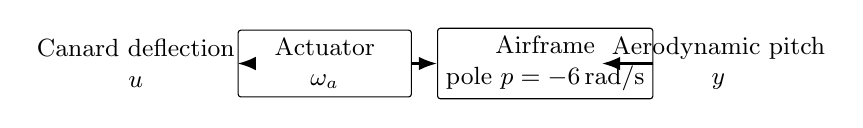
\begin{tikzpicture}[>=Latex,every node/.style={font=\small}]
			\node[align=center] (u) at (-3.4,0) {Canard deflection\\$u$};
			\node[ctlwide] (act) at (-1.0,0) {Actuator\\$\omega_a$};
			\node[ctlwide] (air) at (1.8,0) {Airframe\\pole $p=-6\,\mathrm{rad/s}$};
			\node[align=center] (y) at (4.0,0) {Aerodynamic pitch\\$y$};
			\draw[signal] (u) -- (act);
			\draw[signal] (act) -- (air);
			\draw[signal] (air) -- (y);
		\end{tikzpicture}
		\caption{Simplified actuator-to-airframe path from canard deflection to aerodynamic pitch.}
		\label{fig:canard-airframe-path}
	\end{figure}
	\textit{(The X-29 pitch control channel: Actuator hydraulic rate limits constrain the loop bandwidth relative to the open-loop unstable pole).}
	\paragraph{Sensitivity Analysis via Bode's Integral}
	Using Stein's piecewise sensitivity model with open-loop unstable pole $p$: \[
	\int_{0}^{\infty} \ln |S(j\omega)|\, d\omega = \pi p \quad
	\] Assuming good disturbance rejection ($|S| \le \epsilon$) up to tracking frequency $\omega_1$, bounded peak sensitivity $M_s$ across $[\omega_1, \omega_a]$, and actuator roll-off ($|S| \approx 1$) above hydraulic cutoff frequency $\omega_a$, integration yields: \[
	\ln M_s = \frac{\pi p + \omega_1}{\omega_a} \implies M_s = \exp\left( \frac{\pi p + \omega_1}{\omega_a} \right) \quad
	\]
	\begin{itemize}
		\item
		\textbf{Numerical Evaluation:}
		\begin{itemize}
			\item
			For the X-29 with $p = 6\text{ rad/s}$ and desired control bandwidth $\omega_1 = 3\text{ rad/s}$: \[
			\pi p + \omega_1 = \pi(6) + 3 \approx 18.85 + 3 = 21.85\text{ rad/s}
			\]
			\item
			If hydraulic surface actuators have a bandwidth of $\omega_a = 30\text{ rad/s}$: \[
			M_s = \exp\left( \frac{21.85}{30} \right) = \exp(0.728) \approx 2.07 \quad (\text{acceptable stability margin: } s_m \approx 0.48)
			\]
			\item
			If actuator response drops (due to thermal fade, pressure drop, or rate limits) to $\omega_a = 15\text{ rad/s}$: \[
			M_s = \exp\left( \frac{21.85}{15} \right) = \exp(1.457) \approx 4.29 \quad (\text{fragile margin: } s_m \approx 0.23)
			\]
		\end{itemize}
		\item
		\textbf{The Lesson of "Respect the Unstable":} When controlling open-loop unstable systems, \textbf{feedback requires adequate actuator authority and bandwidth}. If an actuator saturates in velocity or angle, effective loop gain collapses, moving $\omega_a$ inward and causing $M_s \to \infty$, leading to immediate loss of control.
	\end{itemize}
	
	\subsection{Summary Comparison of Week 12 Fundamental Limitation Principles}
	\begin{center}\small\begin{tabularx}{\textwidth}{L{0.8} L{1.1} L{1.1}}
			\toprule
			\textbf{Principle / Concept} & \textbf{Governing Equation / Criterion} & \textbf{Core System-Theoretic Meaning} \\
			\midrule
			\textbf{Passivity (Frequency Domain)} & $\text{Re}[L(j\omega)] \ge 0, \quad \forall \omega$ & Nyquist plot stays in RHP, guaranteeing $\lvert S(j\omega)\rvert \le 1$. \\
			\textbf{Bode Integral (Stable Plants)} & $\int_{0}^{\infty} \ln \lvert S(j\omega)\rvert \, d\omega = 0$ & Waterbed effect: sensitivity attenuation is balanced by an equal area of amplification. \\
			\textbf{Bode Integral (Unstable Plants)} & $\int_{0}^{\infty} \ln \lvert S(j\omega)\rvert \, d\omega = \pi \sum_{p_k > 0} p_k$ & Unstable poles worsen the waterbed: amplification exceeds attenuation by $\pi \sum p_k$. \\
			\textbf{Exponential Peaking Bound} & $M_s \ge \exp\left(\frac{\pi p + \omega_1}{\omega_a - \omega_1}\right) \quad$ & As control bandwidth approaches actuator cutoff, sensitivity peaks exponentially. \\
			\textbf{Maximum Modulus Condition} & $S(z) = 1, \quad T(p) = 1 \implies M_s, M_t \ge 1 \quad$ & Right-half-plane singularities act as interpolation obstacles for sensitivity functions. \\
			\textbf{RHP Pole-Zero Interaction} & $M_s \ge \left\lvert \dfrac{z + p}{z - p} \right\rvert$ & An RHP pole near an RHP zero forces severe sensitivity peaking ($M_s \to \infty$ as $p \to z$). \\
			\textbf{RHP Zero Bandwidth Limit} & $\omega_{sc} \le z \sqrt{\frac{M_s - 1}{M_s + 1}} \quad$ & Non-minimum-phase zeros place an upper bound on achievable closed-loop bandwidth. \\
			\textbf{Time-Delay Limit} & $\omega_{gc} \tau \le \phi_{ap} \quad$ & Linear phase lag from transport delays limits crossover frequency: $\omega_{gc} < 1/\tau$. \\
			\bottomrule
	\end{tabularx}\end{center}
	
	\subsection{MATLAB Script: Demonstrating the Waterbed Effect \& Bode's Integral}
	\begin{lstlisting}
		%% ECE4132 Week 12: Waterbed Effect and Bode Integral Verification
		clear; clc; close all;
		
		% 1. Define Open-Loop Stable Plant
		s = tf('s');
		P = 1 / ((s + 1)*(s + 2));          % Relative degree = 2 (lim s*L = 0)
		
		% 2. Compare Two Controllers: Moderate vs. Aggressive Integral Action
		C_mod = 2 + 1/s;                    % Moderate PI controller
		C_agg = 15 + 25/s;                  % Aggressive PI controller
		
		L_mod = P * C_mod;
		L_agg = P * C_agg;
		
		% 3. Closed-Loop Sensitivity Functions
		S_mod = feedback(1, L_mod);
		S_agg = feedback(1, L_agg);
		
		% 4. Frequency Grid for Integration (Linear scale for Bode's Integral)
		w = linspace(0.001, 100, 50000);   % Linear frequency vector
		[mag_mod, ~] = bode(S_mod, w);
		[mag_agg, ~] = bode(S_agg, w);
		
		log_S_mod = log(squeeze(mag_mod));  % Natural logarithm ln|S(jomega)|
		log_S_agg = log(squeeze(mag_agg));
		
		% 5. Numerical Trapezoidal Integration of Bode's Integral
		integral_mod = trapz(w, log_S_mod);
		integral_agg = trapz(w, log_S_agg);
		
		fprintf('=== Numerical Verification of Bode Integral ===\n');
		fprintf('Theoretical Area for Stable Plant: 0.000\n');
		fprintf('Integrated Area (Moderate PI):    %.4f\n', integral_mod);
		fprintf('Integrated Area (Aggressive PI):  %.4f\n', integral_agg);
		
		% 6. Plot Sensitivity Curves Illustrating the Waterbed Effect
		figure('Name', 'The Waterbed Effect in Sensitivity');
		plot(w, log_S_mod, 'b', 'LineWidth', 1.8); hold on;
		plot(w, log_S_agg, 'r--', 'LineWidth', 1.8);
		yline(0, 'k-', 'LineWidth', 1);
		xlim(); ylim([-4, 1.5]);
		grid on;
		xlabel('Frequency \omega [rad/s] (Linear Scale)');
		ylabel('ln |S(j\omega)|');
		title('Waterbed Effect: Deeper Low-Frequency Attenuation Forces a Higher Peak M_s');
		legend('Moderate Control (Lower M_s)', 'Aggressive Control (High M_s Peak)', '|S| = 1 Line');
		
		% Peak Sensitivity Comparisons
		Ms_mod = norm(S_mod, Inf);
		Ms_agg = norm(S_agg, Inf);
		fprintf('\nPeak Sensitivity Ms (Moderate): %.2f (%.2f dB)\n', Ms_mod, 20*log10(Ms_mod));
		fprintf('Peak Sensitivity Ms (Aggressive): %.2f (%.2f dB)\n', Ms_agg, 20*log10(Ms_agg));
	\end{lstlisting}
	
	\newpage
	\section{Examination Structure \& Prediction Analysis}
	The \textbf{ECE4132 Mock Exam} tests core competencies across five modular themes:
	\begin{enumerate}
		\item
		\textbf{Response Classification \& System Types} (Questions 1 \& 2): Matching loop transfer functions to step/ramp responses and evaluating steady-state error.
		\item
		\textbf{Frequency Domain \& Sensitivity Analysis} (Question 4): Interpreting loop transfer functions $L(s)$, Nyquist encirclements of $-1$, sensitivity peaks $M_s = \max_\omega |S(j\omega)|$, and tracking bandwidth.
		\item
		\textbf{Nonlinear Systems \& Equilibrium Linearisation} (Question 5): Determining multiple equilibrium points for autonomous nonlinear differential equations and computing local Jacobian matrices.
		\item
		\textbf{State-Space Control \& Observer Synthesis} (Question 6): Evaluating internal versus BIBO stability, placing observer eigenvalues ($A - LC$), computing state feedback gains ($A - BK$), and finding the open-loop reference gain $k_r$.
		\item
		\textbf{Physical Modelling \& Digital Implementation} (Questions 3 \& 7): Deriving transfer functions from physical circuits, designing continuous controllers (PI) for transient settling, discretising via Euler methods, and deriving microcontroller difference equations.
	\end{enumerate}
	
	\subsection{Predicted Master Exam Question (25 Marks)}
	\paragraph{Context \& Problem Statement}
	Active magnetic levitation (MagLev) systems are widely used in high-speed rail, magnetic bearings, and frictionless semiconductor manufacturing. A precision magnetic levitation actuator suspends a ferromagnetic sphere of mass $m$ in vertical space using an electromagnet, as shown below:
	\begin{figure}[H]
		\centering
		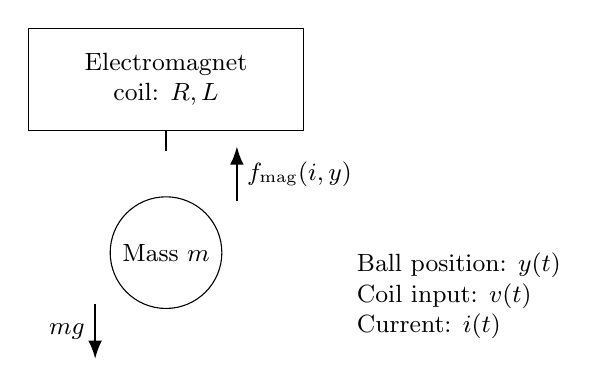
\begin{tikzpicture}[>=Latex,every node/.style={font=\small}]
			\node[draw,rectangle,minimum width=35mm,minimum height=13mm,align=center] (coil) at (0,2.2) {Electromagnet\\coil: $R,L$};
			\node[draw,circle,minimum size=13mm,align=center] (ball) at (0,0) {Mass $m$};
			\draw[thick] (coil.south) -- ++(0,-0.25);
			\draw[signal] (0.9,0.65) -- (0.9,1.35) node[midway,right] {$f_{\mathrm{mag}}(i,y)$};
			\draw[signal] (-0.9,-0.65) -- (-0.9,-1.35) node[midway,left] {$mg$};
			\node[anchor=west,align=left] at (2.3,-0.55) {Ball position: $y(t)$\\Coil input: $v(t)$\\Current: $i(t)$};
		\end{tikzpicture}
		\caption{Electromagnetically suspended ball model: magnetic attraction opposes gravity.}
		\label{fig:suspended-ball-physics}
	\end{figure}
	The vertical position $y(t)$ is measured downward from the electromagnet pole face. The nonlinear equation of motion for the ball and the electrical dynamics of the coil are governed by: \[
	m \frac{d^2 y(t)}{dt^2} = m g - k \frac{i(t)^2}{y(t)^2}
	\] \[
	v(t) = R i(t) + L \frac{di(t)}{dt}
	\]
	where:
	\begin{itemize}
		\item
		Ball mass $m = 1\text{ kg}$, acceleration due to gravity $g = 8\text{ m/s}^2$
		\item
		Electromagnetic force constant $k = 8\text{ N}\cdot\text{m}^2/\text{A}^2$
		\item
		Coil resistance $R = 2,\Omega$, coil inductance $L = 0.5\text{ H}$
		\item
		System input is the applied coil voltage $u(t) = v(t)$
		\item
		Measurable system output is the vertical position $y(t)$
	\end{itemize}
	
	\paragraph{Exam Questions}
	\subparagraph{\textbf{Part (a) Physical Modelling \& Equilibrium Analysis [4 marks]}}
	\begin{enumerate}
		\item
		Show that for a desired steady-state levitation gap of $y_0 = 1\text{ m}$, the required equilibrium bias current is $i_0 = 1\text{ A}$ and the equilibrium input voltage is $v_0 = 2\text{ V}$.
		\item
		Define the state vector $x(t) = \begin{bmatrix} x_1(t) & x_2(t) & x_3(t) \end{bmatrix}^T = \begin{bmatrix} y(t) & \dot{y}(t) & i(t) \end{bmatrix}^T$. Define small perturbation variables around the equilibrium point: $\delta x(t) = x(t) - x_0$ and $\delta u(t) = v(t) - v_0$. Derive the linearized state-space matrices $(A, B, C, D)$ governing the perturbation dynamics $\delta \dot{x} = A \delta x + B \delta u$, $\delta y = C \delta x + D \delta u$.
	\end{enumerate}
	\subparagraph{\textbf{Part (b) Stability \& Transfer Function Analysis [3 marks]}}
	\begin{enumerate}
		\item
		Determine the eigenvalues of $A$ and derive the open-loop transfer function $G(s) = \frac{\Delta Y(s)}{\Delta V(s)}$.
		\item
		Is the open-loop linearized system internally stable? Is it bounded-input bounded-output (BIBO) stable? Explain from physical and mathematical perspectives why open-loop feedforward control cannot maintain stable levitation.
	\end{enumerate}
	\subparagraph{\textbf{Part (c) Full-State Feedback with Integral Tracking Control [5 marks]}}
	In the mock exam, reference tracking was implemented using a static feedforward gain $k_r$.
	\begin{enumerate}
		\item
		Explain why this static feedforward architecture fails when the physical mass $m$ or resistance $R$ undergoes parameter drift, or when a constant external force disturbance acts on the sphere.
		\item
		To achieve zero steady-state error to step position commands despite parameter variations, augment the state space with an integrator: \[
		\dot{x}_I(t) = r(t) - \delta y(t) = r(t) - C \delta x(t)
		\] Define the augmented state vector $x_e(t) = \begin{bmatrix} \delta x(t)^T & x_I(t) \end{bmatrix}^T \in \mathbb{R}^4$. Write down the augmented system matrices $A_e$ and $B_e$.
		\item
		Design a state-feedback gain vector $K_e = \begin{bmatrix} k_1 & k_2 & k_3 & -k_I \end{bmatrix}$ such that all four closed-loop poles are placed at $s = -4$.
	\end{enumerate}
	\subparagraph{\textbf{Part (d) Luenberger State Observer Design \& Separation Principle [4 marks]}}
	In the physical setup, only the vertical displacement $\delta y(t) = \delta x_1(t)$ is measured by an optical sensor; velocity $\delta x_2$ and coil current $\delta x_3$ are not directly measured.
	\begin{enumerate}
		\item
		Prove that the pair $(A, C)$ is observable.
		\item
		Design a full-order Luenberger state observer $\dot{\hat{x}} = A \hat{x} + B \delta u + L(\delta y - C \hat{x})$ such that the observer estimation error dynamics $e_o(t) = \delta x(t) - \hat{x}(t)$ decay with a triple pole at $s = -8$.
		\item
		State the \textbf{Separation Principle}. What are the eigenvalues of the complete 7th-order closed-loop system combining the plant, the integral controller, and the observer?
	\end{enumerate}
	\subparagraph{\textbf{Part (e) Robustness \& Frequency-Domain Performance Trade-offs [4 marks]}}
	\begin{enumerate}
		\item
		Define the \textbf{Sensitivity Function} $S(s)$ and the \textbf{peak sensitivity} $M_s = \sup_{\omega} |S(j\omega)|$. Why does $M_s$ provide a more reliable guarantee of stability margins than classical gain and phase margins?
		\item
		The open-loop plant has an unstable pole in the right-half plane (RHP). State \textbf{Bode's Sensitivity Integral Theorem} (the "Waterbed Effect") for open-loop unstable plants. Explain the fundamental design limitation this imposes on the closed-loop system when attempting to reduce sensitivity over a wide tracking bandwidth.
	\end{enumerate}
	\subparagraph{\textbf{Part (f) Digital Microcontroller Implementation [5 marks]}}
	\begin{enumerate}
		\item
		Compare the \textbf{Forward Euler}, \textbf{Backward Euler}, and \textbf{Bilinear (Tustin)} transform methods for discretising continuous-time compensators. Why is the Tustin transform preferred when digitising controllers with fast dynamics?
		\item
		Using the \textbf{Backward Euler method} with sampling period $T_s$, derive the explicit difference equations that must be executed in real time on the digital signal processor / microcontroller at sample step $k$ to compute the control output $u[k]$ from the reference $r[k]$ and measured position $y[k]$.
		\item
		State the engineering rule of thumb for selecting an appropriate sampling period $T_s$ based on the closed-loop pole locations, and recommend a specific value for this system.
	\end{enumerate}
	
	\subsection{Complete Answer Key \& Marking Guide}
	\paragraph{Solution to Part (a) [4 marks]}
	\textbf{1. Equilibrium Point Derivation [1 mark]} At steady state, all time derivatives vanish: $\ddot{y} = 0$, $\dot{y} = 0$, $\frac{di}{dt} = 0$. From the mechanical equation: \[
	0 = mg - k \frac{i_0^2}{y_0^2} \implies mg = k \left(\frac{i_0}{y_0}\right)^2
	\] Substitute the given numerical parameters $m = 1\text{ kg}$, $g = 8\text{ m/s}^2$, $k = 8\text{ N}\cdot\text{m}^2/\text{A}^2$, and $y_0 = 1\text{ m}$: \[
	1 \times 8 = 8 \left(\frac{i_0}{1}\right)^2 \implies i_0^2 = 1 \implies i_0 = 1\text{ A} \quad (\text{since } i_0 > 0)
	\] From the electrical equation: \[
	v_0 = R i_0 = 2,\Omega \times 1\text{ A} = 2\text{ V}
	\] Thus, the equilibrium state and input are: \[
	x_0 = \begin{bmatrix} y_0 \\ \dot{y}_0 \\ i_0 \end{bmatrix} = \begin{bmatrix} 1 \\ 0 \\ 1 \end{bmatrix}, \quad u_0 = v_0 = 2\text{ V}
	\]
	\textbf{2. Jacobian Linearisation [3 marks]} The nonlinear state equations $\dot{x} = f(x, u)$ are: \[
	f_1(x, u) = x_2
	\] \[
	f_2(x, u) = g - \frac{k}{m} \frac{x_3^2}{x_1^2}
	\] \[
	f_3(x, u) = -\frac{R}{L} x_3 + \frac{1}{L} u
	\]
	Compute the partial derivatives evaluated at $(x_0, u_0)$: \[
	\frac{\partial f_1}{\partial x} = \begin{bmatrix} 0 & 1 & 0 \end{bmatrix}, \quad \frac{\partial f_1}{\partial u} = 0
	\] \[
	\frac{\partial f_2}{\partial x_1} = \frac{2k x_3^2}{m x_1^3}\Bigg|_{x_0} = \frac{2(8)(1)^2}{(1)(1)^3} = 16, \quad \frac{\partial f_2}{\partial x_2} = 0
	\] \[
	\frac{\partial f_2}{\partial x_3} = -\frac{2k x_3}{m x_1^2}\Bigg|_{x_0} = -\frac{2(8)(1)}{(1)(1)^2} = -16, \quad \frac{\partial f_2}{\partial u} = 0
	\] \[
	\frac{\partial f_3}{\partial x_1} = 0, \quad \frac{\partial f_3}{\partial x_2} = 0, \quad \frac{\partial f_3}{\partial x_3} = -\frac{R}{L} = -\frac{2}{0.5} = -4, \quad \frac{\partial f_3}{\partial u} = \frac{1}{L} = \frac{1}{0.5} = 2
	\]
	Since the output is vertical position $\delta y = \delta x_1$: \[
	C = \begin{bmatrix} 1 & 0 & 0 \end{bmatrix}, \quad D = 0
	\] The linearized state-space matrices are: \[
	A = \begin{bmatrix} 0 & 1 & 0 \\ 16 & 0 & -16 \\ 0 & 0 & -4 \end{bmatrix}, \quad B = \begin{bmatrix} 0 \\ 0 \\ 2 \end{bmatrix}, \quad C = \begin{bmatrix} 1 & 0 & 0 \end{bmatrix}, \quad D = 0
	\]
	
	\paragraph{Solution to Part (b) [3 marks]}
	\textbf{1. Eigenvalues and Transfer Function [2 marks]} Compute the characteristic polynomial of $A$: \[
	\det(sI - A) = \det\begin{bmatrix} s & -1 & 0 \\ -16 & s & 16 \\ 0 & 0 & s + 4 \end{bmatrix} = (s + 4) \left( s^2 - 16 \right) = (s + 4)^2 (s - 4) = s^3 + 4s^2 - 16s - 64
	\] The open-loop eigenvalues are: \[
	\lambda_1 = +4, \quad \lambda_2 = -4, \quad \lambda_3 = -4
	\] To find the transfer function $G(s) = C(sI - A)^{-1} B$: \[
	(sI - A) X(s) = B U(s) \implies \begin{bmatrix} s & -1 & 0 \\ -16 & s & 16 \\ 0 & 0 & s + 4 \end{bmatrix} \begin{bmatrix} X_1(s) \\ X_2(s) \\ X_3(s) \end{bmatrix} = \begin{bmatrix} 0 \\ 0 \\ 2 \end{bmatrix} U(s)
	\] From the third row: $X_3(s) = \frac{2}{s + 4} U(s)$. From the first row: $X_2(s) = s X_1(s)$. Substitute into the second row: \[
	-16 X_1(s) + s(s X_1(s)) + 16 X_3(s) = 0 \implies (s^2 - 16) X_1(s) = -16 X_3(s) = -\frac{32}{s + 4} U(s)
	\] \[
	X_1(s) = \frac{-32}{(s^2 - 16)(s + 4)} U(s) = \frac{-32}{(s - 4)(s + 4)^2} U(s)
	\] Because $Y(s) = X_1(s)$, the transfer function is: \[
	G(s) = \frac{-32}{s^3 + 4s^2 - 16s - 64}
	\]
	\textbf{2. Stability Discussion [1 mark]}
	\begin{itemize}
		\item
		\textbf{Internal Stability:} The system is \textbf{internally unstable} because there is an eigenvalue $\lambda_1 = +4$ in the open right-half plane ($\text{Re}(\lambda) > 0$).
		\item
		\textbf{BIBO Stability:} The transfer function possesses an uncancelled pole at $s = +4 \in \text{ORHP}$, so the system is \textbf{not BIBO stable}.
		\item
		\textbf{Physical Failure of Feedforward:} Open-loop feedforward cannot stabilize this plant. Because the magnetic force is inversely proportional to $y^2$, an infinitesimal upward displacement increases the upward magnetic force, accelerating the ball into the magnet; an infinitesimal downward displacement decreases the magnetic force, causing the ball to fall under gravity. The mode $e^{+4t}$ diverges exponentially to infinity without feedback.
	\end{itemize}
	
	\paragraph{Solution to Part (c) [5 marks]}
	\textbf{1. Failure of Open-Loop Reference Gain $k_r$ [1 mark]} In the static state-feedback architecture $u = -K x + k_r r$, the steady-state tracking gain is derived from the model nominal matrices: $k_r = -[C(A - BK)^{-1}B]^{-1}$. This constitutes open-loop inversion. Any mismatch between the true physical plant and the model (e.g., changes in mass $m$, coil heating altering $R$, or an external wind/load disturbance $v(t)$) causes the DC gain to shift away from unity, resulting in steady-state error ($e_{ss} \neq 0$).
	\textbf{2. Augmented State-Space Formulation [1 mark]} Introducing the integrator state $\dot{x}_I(t) = r(t) - C \delta x(t)$ forces $e(t) = r(t) - y(t) \to 0$ at steady state via the Internal Model Principle. The augmented state equations are: \[
	\begin{bmatrix} \delta \dot{x} \\ \dot{x}_I \end{bmatrix} = \begin{bmatrix} A & 0_{3 \times 1} \\ -C & 0 \end{bmatrix} \begin{bmatrix} \delta x \\ x_I \end{bmatrix} + \begin{bmatrix} B \\ 0 \end{bmatrix} \delta u + \begin{bmatrix} 0_{3 \times 1} \\ 1 \end{bmatrix} r
	\] \[
	A_e = \begin{bmatrix} 0 & 1 & 0 & 0 \\ 16 & 0 & -16 & 0 \\ 0 & 0 & -4 & 0 \\ -1 & 0 & 0 & 0 \end{bmatrix}, \quad B_e = \begin{bmatrix} 0 \\ 0 \\ 2 \\ 0 \end{bmatrix}
	\]
	\textbf{3. State Feedback Gain Computation [3 marks]} The feedback law is: \[
	\delta u = -K \delta x + k_I x_I = -K_e x_e, \quad \text{where } K_e = \begin{bmatrix} k_1 & k_2 & k_3 & -k_I \end{bmatrix}
	\] The closed-loop dynamics matrix is: \[
	A_e - B_e K_e = \begin{bmatrix} 0 & 1 & 0 & 0 \\ 16 & 0 & -16 & 0 \\ -2k_1 & -2k_2 & -4 - 2k_3 & 2k_I \\ -1 & 0 & 0 & 0 \end{bmatrix}
	\] Evaluate the closed-loop characteristic polynomial: \[
	\det(sI - (A_e - B_e K_e)) = s^4 + (2k_3 + 4)s^3 - (32k_2 + 16)s^2 - (32k_1 + 32k_3 + 64)s - 32k_I
	\] The desired closed-loop polynomial with four poles at $s = -4$ is: \[
	\alpha_d(s) = (s + 4)^4 = s^4 + 16s^3 + 96s^2 + 256s + 256
	\] Equating coefficients term-by-term:
	\begin{itemize}
		\item
		Coefficient of $s^3$: \[
		2k_3 + 4 = 16 \implies 2k_3 = 12 \implies \mathbf{k_3 = 6}
		\]
		\item
		Coefficient of $s^2$: \[
		-32k_2 - 16 = 96 \implies -32k_2 = 112 \implies \mathbf{k_2 = -3.5 = -\frac{7}{2}}
		\]
		\item
		Constant term ($s^0$): \[
		-32k_I = 256 \implies \mathbf{k_I = -8}
		\]
		\item
		Coefficient of $s^1$: \[
		-32k_1 - 32k_3 - 64 = 256 \implies -32k_1 - 32(6) - 64 = 256
		\] \[
		-32k_1 - 256 = 256 \implies -32k_1 = 512 \implies \mathbf{k_1 = -16}
		\]
	\end{itemize}
	The feedback gain vector is: \[
	K_e = \begin{bmatrix} -16 & -3.5 & 6 & 8 \end{bmatrix}
	\] The resulting continuous control law is: \[
	\delta u(t) = 16 \delta x_1(t) + 3.5 \delta x_2(t) - 6 \delta x_3(t) - 8 x_I(t)
	\]
	
	\paragraph{Solution to Part (d) [4 marks]}
	\textbf{1. Observability Rank Test [1 mark]} The observability matrix $W_o$ is: \[
	W_o = \begin{bmatrix} C \\ CA \\ CA^2 \end{bmatrix} = \begin{bmatrix} 1 & 0 & 0 \\ 0 & 1 & 0 \\ 16 & 0 & -16 \end{bmatrix}
	\] \[
	\det(W_o) = 1 \times (1 \times (-16) - 0) = -16 \neq 0
	\] Since $\text{rank}(W_o) = 3 = n$, the system is completely observable.
	\textbf{2. Observer Gain Computation [2 marks]} The observer dynamics matrix is $A - LC$, where $L = \begin{bmatrix} l_1 & l_2 & l_3 \end{bmatrix}^T$: \[
	A - LC = \begin{bmatrix} 0 & 1 & 0 \\ 16 & 0 & -16 \\ 0 & 0 & -4 \end{bmatrix} - \begin{bmatrix} l_1 & 0 & 0 \\ l_2 & 0 & 0 \\ l_3 & 0 & 0 \end{bmatrix} = \begin{bmatrix} -l_1 & 1 & 0 \\ 16 - l_2 & 0 & -16 \\ -l_3 & 0 & -4 \end{bmatrix}
	\] Compute $\det(sI - (A - LC))$: \[
	\det\begin{bmatrix} s + l_1 & -1 & 0 \\ l_2 - 16 & s & 16 \\ l_3 & 0 & s + 4 \end{bmatrix} = (s + l_1)s(s + 4) + (l_2 - 16)(s + 4) - 16 l_3
	\] \[
	= s^3 + (l_1 + 4)s^2 + (4l_1 + l_2 - 16)s + (4l_2 - 16l_3 - 64)
	\] The target observer characteristic polynomial with triple pole at $s = -8$ is: \[
	\beta_d(s) = (s + 8)^3 = s^3 + 24s^2 + 192s + 512
	\] Equating coefficients:
	\begin{itemize}
		\item
		$s^2$ term: \[
		l_1 + 4 = 24 \implies \mathbf{l_1 = 20}
		\]
		\item
		$s^1$ term: \[
		4l_1 + l_2 - 16 = 192 \implies 4(20) + l_2 - 16 = 192 \implies 64 + l_2 = 192 \implies \mathbf{l_2 = 128}
		\]
		\item
		Constant term ($s^0$): \[
		4l_2 - 16l_3 - 64 = 512 \implies 4(128) - 16l_3 - 64 = 512
		\] \[
		512 - 16l_3 - 64 = 512 \implies -16l_3 = 64 \implies \mathbf{l_3 = -4}
		\]
	\end{itemize}
	The observer gain matrix is: \[
	L = \begin{bmatrix} 20 \\ 128 \\ -4 \end{bmatrix}
	\]
	\textbf{3. The Separation Principle \& Closed-Loop Poles [1 mark]}
	\begin{itemize}
		\item
		\textbf{Statement:} For a linear time-invariant system, the state feedback gains $K_e$ and the observer gains $L$ can be designed completely independently. The closed-loop poles of the combined output-feedback system are the eigenvalues of $(A_e - B_e K_e)$ along with the eigenvalues of $(A - LC)$.
		\item
		\textbf{Eigenvalues:} The composite 7th-order system ($3$ plant states + $1$ integrator state + $3$ observer estimation error states) has closed-loop eigenvalues: \[
		\lambda_{cl} = { -4, -4, -4, -4, -8, -8, -8 }
		\]
	\end{itemize}
	
	\paragraph{Solution to Part (e) [4 marks]}
	\textbf{1. Sensitivity Peak $M_s$ vs. Classical Margins [2 marks]} The sensitivity function is $S(s) = \frac{1}{1 + L(s)}$, where $L(s)$ is the open-loop return ratio. The peak sensitivity is defined as: \[
	M_s = \sup_{\omega \ge 0} |S(j\omega)| = \frac{1}{\inf_{\omega} |1 + L(j\omega)|}
	\] Geometrically, $|1 + L(j\omega)|$ is the distance from the Nyquist trajectory $L(j\omega)$ to the critical point $-1$ in the complex plane. Therefore: \[
	\text{Distance to }-1 = \frac{1}{M_s}
	\]
	\begin{itemize}
		\item
		Classical \textbf{Gain Margin (GM)} only tests distance to $-1$ along the negative real axis (where phase is $-180^\circ$).
		\item
		Classical \textbf{Phase Margin (PM)} only tests distance to $-1$ along the unit circle (where magnitude is $1$).
		\item
		\textbf{Why $M_s$ is superior:} A system can have high GM and PM while the Nyquist curve passes dangerously close to $-1$ at an intermediate angle. The metric $M_s$ accounts for simultaneous magnitude and phase uncertainties: \[
		GM \ge \frac{M_s}{M_s - 1}, \quad PM \ge 2 \arcsin\left(\frac{1}{2M_s}\right)
		\]
	\end{itemize}
	\textbf{2. Bode's Sensitivity Integral \& The Waterbed Effect [2 marks]} For an open-loop plant with relative degree $\ge 2$ and open-loop unstable poles $p_k \in \text{ORHP}$, Bode's Sensitivity Integral states: \[
	\int_{0}^{\infty} \ln |S(j\omega)|\, d\omega = \pi \sum_{k} \text{Re}(p_k)
	\] For this MagLev plant, there is an open-loop unstable pole at $p_1 = +4$: \[
	\int_{0}^{\infty} \ln |S(j\omega)|\, d\omega = 4\pi > 0
	\]
	\begin{itemize}
		\item
		\textbf{Fundamental Limitation:} To achieve accurate tracking and disturbance rejection over the control bandwidth $[0, \omega_B]$, we require $|S(j\omega)| < 1$, which makes $\ln |S(j\omega)| < 0$ (a sensitivity "valley").
		\item
		Because the total area under $\ln |S(j\omega)|$ across all frequencies is fixed to $+4\pi$, pressing down sensitivity at low frequencies forces a severe amplification $|S(j\omega)| > 1$ ($\ln |S| > 0$) at higher frequencies (a sensitivity "peak").
		\item
		This fundamental trade-off means that improving tracking performance inevitably worsens high-frequency noise amplification and reduces robustness margins.
	\end{itemize}
	
	\paragraph{Solution to Part (f) [5 marks]}
	\textbf{1. Comparison of Discretisation Operators [1 mark]}
	\begin{itemize}
		\item
		\textbf{Forward Euler ($s \approx \frac{z - 1}{T_s}$):} Maps the open left-half $s$-plane into a circle of radius $\frac{1}{T_s}$ centered at $z = 1 - \frac{1}{T_s}$. Stable continuous poles with large negative real parts (such as the observer poles at $-8$) will map outside the unit disk $|z| > 1$ if $T_s > \frac{2}{|\text{pole}|}$, making the discrete implementation unstable.
		\item
		\textbf{Backward Euler ($s \approx \frac{1 - z^{-1}}{T_s}$):} Maps the open left-half $s$-plane into the interior of a circle inside the unit disk. Stability is always preserved, but it adds artificial numerical damping.
		\item
		\textbf{Bilinear / Tustin Transform ($s \approx \frac{2}{T_s} \frac{1 - z^{-1}}{1 + z^{-1}}$):} A conformal mapping that maps the entire open left-half $s$-plane directly onto the open unit disk in the $z$-plane ($|z| < 1$). It unconditionally preserves continuous-time stability without adding artificial damping, making it the preferred method for digital controllers.
	\end{itemize}
	\textbf{2. Microcontroller Real-Time Difference Equations [3 marks]} Using Backward Euler ($s \to \frac{1 - z^{-1}}{T_s}$):
	\begin{enumerate}
		\item
		\textbf{Integrator update:} \[
		\frac{x_I[k] - x_I[k-1]}{T_s} = r[k] - y[k] \implies \mathbf{x_I[k] = x_I[k-1] + T_s \left( r[k] - y[k] \right)}
		\]
		\item
		\textbf{Observer state estimation:} \[
		\hat{x}[k] = \hat{x}[k-1] + T_s \left[ (A - LC) \hat{x}[k-1] + B \delta u[k-1] + L y[k-1] \right]
		\] Substituting the matrices from Parts (a), (c), and (d): \[
		(A - LC) = \begin{bmatrix} -20 & 1 & 0 \\ -112 & 0 & -16 \\ 4 & 0 & -4 \end{bmatrix}, \quad B = \begin{bmatrix} 0 \\ 0 \\ 2 \end{bmatrix}, \quad L = \begin{bmatrix} 20 \\ 128 \\ -4 \end{bmatrix}
		\] Expanding into scalar update equations: \[
		\mathbf{\hat{x}_1[k] = \hat{x}_1[k-1] + T_s \left( -20 \hat{x}_1[k-1] + \hat{x}_2[k-1] + 20 y[k-1] \right)}
		\] \[
		\mathbf{\hat{x}_2[k] = \hat{x}_2[k-1] + T_s \left( -112 \hat{x}_1[k-1] - 16 \hat{x}_3[k-1] + 128 y[k-1] \right)}
		\] \[
		\mathbf{\hat{x}_3[k] = \hat{x}_3[k-1] + T_s \left( 4 \hat{x}_1[k-1] - 4 \hat{x}_3[k-1] + 2 \delta u[k-1] - 4 y[k-1] \right)}
		\]
		\item
		\textbf{Control output computation:} \[
		\delta u[k] = 16 \hat{x}_1[k] + 3.5 \hat{x}_2[k] - 6 \hat{x}_3[k] - 8 x_I[k]
		\] \[
		u_{total}[k] = v_0 + \delta u[k] = \mathbf{2 + 16 \hat{x}_1[k] + 3.5 \hat{x}_2[k] - 6 \hat{x}_3[k] - 8 x_I[k]}
		\]
	\end{enumerate}
	\textbf{3. Sampling Period Selection [1 mark]}
	\begin{itemize}
		\item
		\textbf{Rule of Thumb:} To avoid excessive digital phase lag and sampling-induced destabilization, the sampling frequency $\omega_s = \frac{2\pi}{T_s}$ should be selected between $20$ and $40$ times higher than the highest bandwidth or pole magnitude of the closed-loop system: \[
		\omega_s \ge 20 \times \max_i |\lambda_i| \implies T_s \le \frac{2\pi}{20 \times |\lambda_{max}|} \approx \frac{1}{3 \times |\lambda_{max}|}
		\]
		\item
		For this closed-loop system, the fastest poles are the observer poles at $|\lambda| = 8\text{ rad/s}$. \[
		T_s \le \frac{2\pi}{20 \times 8} \approx 0.039\text{ s}
		\]
		\item
		\textbf{Recommendation:} Select $\mathbf{T_s = 0.01\text{ s}}$ ($10\text{ ms}$, corresponding to a sampling rate of $100\text{ Hz}$). This is well within the capability of standard microcontrollers (e.g., STM32, ARM Cortex-M) and ensures that continuous-time design assumptions remain valid.
	\end{itemize}
	
	\subsection{Key Formulas \& Verification Summary}
	\begin{center}\small\begin{tabularx}{\textwidth}{*{3}{Y}}
			\toprule
			\textbf{Component} & \textbf{Continuous System} & \textbf{Synthesized Value / Characteristic} \\
			\midrule
			\textbf{Equilibrium} & $(y_0, \dot{y}_0, i_0, v_0)$ & $(1\text{ m}, 0\text{ m/s}, 1\text{ A}, 2\text{ V})$ \\
			\textbf{Open-Loop Poles} & $\det(sI - A) = 0$ & $s = +4\text{ (unstable)}, -4, -4$ \\
			\textbf{Plant Transfer Function} & $G(s) = \frac{\Delta Y(s)}{\Delta V(s)}$ & $\frac{-32}{(s - 4)(s + 4)^2}$ \\
			\textbf{Controller Gains} & $K_e = [k_1, k_2, k_3, -k_I]$ & $[-16, -3.5, 6, 8]$ (Closed-loop poles at $-4$) \\
			\textbf{Observer Gains} & $L = [l_1, l_2, l_3]^T$ & $[20, 128, -4]^T$ (Observer poles at $-8$) \\
			\textbf{Bode Sensitivity Integral} & $\int_0^\infty \ln \|S(j\omega)\|$ &  \\
			\textbf{Sampling Interval} & $T_s$ & $0.01\text{ s}$ ($100\text{ Hz}$) \\
			\bottomrule
	\end{tabularx}\end{center}
	\newpage
	
	\section{Exam Review Problem: The Inverted Pendulum Balancing Mechanism}
	\subsection{Problem Context \& Specifications}
	An inverted pendulum apparatus mounted on a motorized pivot is operated around its upright vertical equilibrium. Let $x_1(t) = \theta(t)$ represent the angular deflection (in radians) from the upright position, and let $x_2(t) = \dot{\theta}(t)$ represent the angular velocity. The input $u(t)$ is the horizontal pivot acceleration.
	The continuous-time linearised perturbation equations of motion are given by: \[
	\dot{x}_1(t) = x_2(t)
	\] \[
	\dot{x}_2(t) = x_1(t) + u(t)
	\] \[
	y(t) = x_1(t)
	\]
	Only the angular position $y(t) = \theta(t)$ is measured by a shaft encoder; angular velocity $x_2(t)$ is unmeasured.
	
	\subsubsection{Multi-Part Exam Questions}
	\begin{enumerate}
		\item
		\textbf{State-Space Modeling \& Frequency-Domain Realisation (Week 7):}
		\begin{itemize}
			\item
			Write down the matrices $(A, B, C, D)$ of the state-space model.
			\item
			Calculate the eigenvalues of the system dynamics matrix $A$ and assess open-loop internal stability.
			\item
			Compute the resolvent matrix $(sI - A)^{-1}$ and derive the open-loop transfer function $P(s) = \frac{Y(s)}{U(s)}$.
		\end{itemize}
		\item
		\textbf{Reachability Analysis \& Full-State Feedback Design (Week 8):}
		\begin{itemize}
			\item
			Construct the reachability matrix $W_r$ and verify whether the pair $(A, B)$ is reachable.
			\item
			Design a full-state feedback gain vector $K = \begin{bmatrix} k_1 & k_2 \end{bmatrix}$ such that the closed-loop system poles are assigned to $s_{1,2} = -2 \pm j2$.
			\item
			Compute the feedforward precompensation gain $k_r$ to ensure unity steady-state tracking gain ($y_{ss} = r_{ss}$) for constant setpoint commands.
		\end{itemize}
		\item
		\textbf{Observability \& Luenberger State Estimator Design (Week 9):}
		\begin{itemize}
			\item
			Construct the observability matrix $W_o$ and verify whether the pair $(A, C)$ is observable.
			\item
			Design a Luenberger observer gain vector $L = \begin{bmatrix} l_1 \\ l_2 \end{bmatrix}$ to place both observer error poles at $s_{o1,2} = -5$.
			\item
			State the \textbf{Separation Principle} and write down the composite 4th-order closed-loop characteristic polynomial.
			\item
			Derive the dynamic feedback compensator transfer function $C_{\text{ctrl}}(s) = \frac{U(s)}{-Y(s)}$.
		\end{itemize}
		\item
		\textbf{Loop Frequency Response \& The Gang of Four (Week 10):}
		\begin{itemize}
			\item
			Formulate the open-loop transfer function $L(s) = P(s)C_{\text{ctrl}}(s)$.
			\item
			Formulate the \textbf{Sensitivity Function} $S(s)$ and \textbf{Complementary Sensitivity Function} $T(s)$.
			\item
			Verify that the closed-loop denominator matches the expected poles from the Separation Principle.
		\end{itemize}
		\item
		\textbf{Nyquist Stability Criterion \& Robust Stability (Week 11):}
		\begin{itemize}
			\item
			Identify the number of open-loop right-half-plane poles $P$ of the loop transfer function $L(s)$.
			\item
			Determine the required number of net clockwise encirclements $N$ of the critical point $-1 + j0$ for closed-loop stability using Cauchy's Argument Principle.
			\item
			Express the robust stability condition under multiplicative plant uncertainty $\delta(s)$ using the Small Gain Theorem.
		\end{itemize}
		\item
		\textbf{Fundamental Limitations \& Bode's Integral (Week 12):}
		\begin{itemize}
			\item
			Apply the \textbf{Generalized Bode Sensitivity Integral} to this system and evaluate the exact integral area: \[
			\int_{0}^{\infty} \ln |S(j\omega)|\, d\omega
			\]
			\item
			Explain why the unstable pole at $s = +1$ creates a non-zero lower bound on peak sensitivity $M_s$.
		\end{itemize}
	\end{enumerate}
	
	\subsection{Detailed Step-by-Step Solutions \& Reasoning}
	
	\subsubsection{Part 1: State-Space Modeling \& Transfer Function (Week 7)}
	\paragraph{Matrix Formulation}
	From the linearised differential equations: \[
	\begin{bmatrix} \dot{x}_1(t) \\ \dot{x}_2(t) \end{bmatrix} = \begin{bmatrix} 0 & 1 \\ 1 & 0 \end{bmatrix} \begin{bmatrix} x_1(t) \\ x_2(t) \end{bmatrix} + \begin{bmatrix} 0 \\ 1 \end{bmatrix} u(t)
	\] \[
	y(t) = \begin{bmatrix} 1 & 0 \end{bmatrix} \begin{bmatrix} x_1(t) \\ x_2(t) \end{bmatrix}
	\]
	Thus: \[
	A = \begin{bmatrix} 0 & 1 \\ 1 & 0 \end{bmatrix}, \quad B = \begin{bmatrix} 0 \\ 1 \end{bmatrix}, \quad C = \begin{bmatrix} 1 & 0 \end{bmatrix}, \quad D = 0
	\]
	\paragraph{Eigenvalue and Stability Analysis}
	The characteristic polynomial of $A$ is: \[
	\det(sI - A) = \det \begin{bmatrix} s & -1 \\ -1 & s \end{bmatrix} = s^2 - 1 = (s - 1)(s + 1) = 0
	\]
	\begin{itemize}
		\item
		The eigenvalues of the open-loop matrix $A$ are: \[
		\lambda_1 = +1, \quad \lambda_2 = -1
		\]
		\item
		\textbf{Internal Stability Check:} Because $\lambda_1 = +1 > 0$ resides strictly in the right-half plane, the unforced pendulum equilibrium is \textbf{internally unstable}.
	\end{itemize}
	\paragraph{Resolvent Matrix \& Plant Transfer Function}
	Compute the resolvent $(sI - A)^{-1}$: \[
	(sI - A)^{-1} = \frac{1}{s^2 - 1} \begin{bmatrix} s & 1 \\ 1 & s \end{bmatrix}
	\]
	Using the transfer function formula $P(s) = C(sI - A)^{-1}B + D$: \[
	P(s) = \begin{bmatrix} 1 & 0 \end{bmatrix} \left( \frac{1}{s^2 - 1} \begin{bmatrix} s & 1 \\ 1 & s \end{bmatrix} \right) \begin{bmatrix} 0 \\ 1 \end{bmatrix} = \frac{1}{s^2 - 1} \begin{bmatrix} 1 & 0 \end{bmatrix} \begin{bmatrix} 1 \\ s \end{bmatrix} = \frac{1}{s^2 - 1}
	\]
	The plant has an unstable open-loop pole at $s = +1$ and a stable open-loop pole at $s = -1$.
	
	\subsubsection{Part 2: Reachability \& Full-State Feedback Design (Week 8)}
	\paragraph{Reachability Verification}
	Compute the Reachability Matrix $W_r$: \[
	AB = \begin{bmatrix} 0 & 1 \\ 1 & 0 \end{bmatrix} \begin{bmatrix} 0 \\ 1 \end{bmatrix} = \begin{bmatrix} 1 \\ 0 \end{bmatrix}
	\] \[
	W_r = \begin{bmatrix} B & AB \end{bmatrix} = \begin{bmatrix} 0 & 1 \\ 1 & 0 \end{bmatrix}
	\]
	Evaluating the determinant: \[
	\det(W_r) = (0)(0) - (1)(1) = -1 \neq 0 \implies \text{rank}(W_r) = 2
	\] Because $\text{rank}(W_r) = n = 2$, the system is \textbf{completely reachable}. All closed-loop eigenvalues can be placed at arbitrary complex conjugate locations.
	\paragraph{State Feedback Gain Computation}
	The desired closed-loop poles are $s_{1,2} = -2 \pm j2$. The target closed-loop characteristic polynomial is: \[
	\alpha_d(s) = (s - (-2 + j2))(s - (-2 - j2)) = (s + 2)^2 + 4 = s^2 + 4s + 8
	\]
	Let $K = \begin{bmatrix} k_1 & k_2 \end{bmatrix}$. The closed-loop dynamics matrix is: \[
	A - BK = \begin{bmatrix} 0 & 1 \\ 1 & 0 \end{bmatrix} - \begin{bmatrix} 0 \\ 1 \end{bmatrix} \begin{bmatrix} k_1 & k_2 \end{bmatrix} = \begin{bmatrix} 0 & 1 \\ 1 - k_1 & -k_2 \end{bmatrix}
	\]
	Its characteristic equation is: \[
	\det(sI - (A - BK)) = \det \begin{bmatrix} s & -1 \\ k_1 - 1 & s + k_2 \end{bmatrix} = s(s + k_2) + (k_1 - 1) = s^2 + k_2 s + (k_1 - 1)
	\]
	Equating coefficients with $\alpha_d(s) = s^2 + 4s + 8$: \[
	k_2 = 4
	\] \[
	k_1 - 1 = 8 \implies k_1 = 9
	\]
	Therefore, the state feedback gain vector is: \[
	K = \begin{bmatrix} 9 & 4 \end{bmatrix}
	\]
	\paragraph{Reference Precompensation Gain ($k_r$)}
	To ensure zero steady-state tracking error ($y_{ss} = r_{ss}$), the feedforward gain is set to the reciprocal of the closed-loop DC gain: \[
	k_r = -\frac{1}{C(A - BK)^{-1}B}
	\]
	Evaluating $(A - BK)^{-1}$: \[
	A - BK = \begin{bmatrix} 0 & 1 \\ -8 & -4 \end{bmatrix} \implies (A - BK)^{-1} = \frac{1}{0 - (-8)} \begin{bmatrix} -4 & -1 \\ 8 & 0 \end{bmatrix} = \frac{1}{8} \begin{bmatrix} -4 & -1 \\ 8 & 0 \end{bmatrix}
	\] \[
	C(A - BK)^{-1}B = \begin{bmatrix} 1 & 0 \end{bmatrix} \left( \frac{1}{8} \begin{bmatrix} -4 & -1 \\ 8 & 0 \end{bmatrix} \right) \begin{bmatrix} 0 \\ 1 \end{bmatrix} = \begin{bmatrix} 1 & 0 \end{bmatrix} \begin{bmatrix} -1/8 \\ 0 \end{bmatrix} = -\frac{1}{8}
	\]
	Thus: \[
	k_r = -\frac{1}{-1/8} = 8
	\]
	
	\subsubsection{Part 3: Observability \& Observer-Based Controller (Week 9)}
	\paragraph{Observability Verification}
	Compute the Observability Matrix $W_o$: \[
	CA = \begin{bmatrix} 1 & 0 \end{bmatrix} \begin{bmatrix} 0 & 1 \\ 1 & 0 \end{bmatrix} = \begin{bmatrix} 0 & 1 \end{bmatrix}
	\] \[
	W_o = \begin{bmatrix} C \\ CA \end{bmatrix} = \begin{bmatrix} 1 & 0 \\ 0 & 1 \end{bmatrix}
	\]
	\[
	\det(W_o) = 1 \neq 0 \implies \text{rank}(W_o) = 2
	\] The pair $(A, C)$ is \textbf{completely observable}.
	\paragraph{Observer Gain Synthesis}
	Desired observer error poles are placed at $s_{o1,2} = -5$. The desired observer characteristic polynomial is: \[
	\alpha_o(s) = (s + 5)^2 = s^2 + 10s + 25
	\]
	Let $L = \begin{bmatrix} l_1 \\ l_2 \end{bmatrix}$. The observer error dynamics matrix is: \[
	A - LC = \begin{bmatrix} 0 & 1 \\ 1 & 0 \end{bmatrix} - \begin{bmatrix} l_1 \\ l_2 \end{bmatrix} \begin{bmatrix} 1 & 0 \end{bmatrix} = \begin{bmatrix} -l_1 & 1 \\ 1 - l_2 & 0 \end{bmatrix}
	\]
	Its characteristic equation is: \[
	\det(sI - (A - LC)) = \det \begin{bmatrix} s + l_1 & -1 \\ l_2 - 1 & s \end{bmatrix} = s(s + l_1) + (l_2 - 1) = s^2 + l_1 s + (l_2 - 1)
	\]
	Matching coefficients with $\alpha_o(s) = s^2 + 10s + 25$: \[
	l_1 = 10
	\] \[
	l_2 - 1 = 25 \implies l_2 = 26
	\]
	Thus, the observer gain vector is: \[
	L = \begin{bmatrix} 10 \\ 26 \end{bmatrix}
	\]
	\paragraph{The Separation Principle}
	By the \textbf{Separation Principle}, the $2n = 4$ closed-loop eigenvalues of the observer-based feedback system split into the independent union of controller poles and observer poles: \[
	\det \left( sI - \begin{bmatrix} A - BK & BK \\ 0 & A - LC \end{bmatrix} \right) = \det(sI - (A - BK)) \cdot \det(sI - (A - LC)) = \alpha_d(s) \cdot \alpha_o(s)
	\]
	The composite 4th-order closed-loop characteristic polynomial is: \[
	\Delta_{cl}(s) = (s^2 + 4s + 8)(s^2 + 10s + 25) = s^4 + 14s^3 + 73s^2 + 180s + 200
	\]
	\paragraph{Dynamic Controller Transfer Function}
	Eliminating the estimated state vector $\hat{x}(t)$ gives the feedback compensator transfer function: \[
	C_{\text{ctrl}}(s) = K \left( sI - (A - BK - LC) \right)^{-1} L
	\]
	Calculate the internal dynamics matrix: \[
	A - BK - LC = \begin{bmatrix} 0 & 1 \\ 1 & 0 \end{bmatrix} - \begin{bmatrix} 0 & 0 \\ 9 & 4 \end{bmatrix} - \begin{bmatrix} 10 & 0 \\ 26 & 0 \end{bmatrix} = \begin{bmatrix} -10 & 1 \\ -34 & -4 \end{bmatrix}
	\]
	Invert the resolvent matrix: \[
	sI - (A - BK - LC) = \begin{bmatrix} s + 10 & -1 \\ 34 & s + 4 \end{bmatrix}
	\] \[
	\det(sI - (A - BK - LC)) = (s + 10)(s + 4) - (-34) = s^2 + 14s + 74
	\] \[
	(sI - (A - BK - LC))^{-1} = \frac{1}{s^2 + 14s + 74} \begin{bmatrix} s + 4 & 1 \\ -34 & s + 10 \end{bmatrix}
	\]
	Multiply by $L$ and $K$: \[
	\begin{bmatrix} s + 4 & 1 \\ -34 & s + 10 \end{bmatrix} \begin{bmatrix} 10 \\ 26 \end{bmatrix} = \begin{bmatrix} 10s + 66 \\ 26s - 80 \end{bmatrix}
	\] \[
	C_{\text{ctrl}}(s) = \begin{bmatrix} 9 & 4 \end{bmatrix} \left( \frac{1}{s^2 + 14s + 74} \begin{bmatrix} 10s + 66 \\ 26s - 80 \end{bmatrix} \right) = \frac{9(10s + 66) + 4(26s - 80)}{s^2 + 14s + 74}
	\] \[
	C_{\text{ctrl}}(s) = \frac{194s + 274}{s^2 + 14s + 74}
	\]
	The controller poles are the roots of $s^2 + 14s + 74 = (s + 7)^2 + 25 = 0 \implies s = -7 \pm j5$ (the compensator is open-loop stable).
	
	\subsubsection{Part 4: Frequency Response \& The Gang of Four (Week 10)}
	\paragraph{Loop Transfer Function $L(s)$}
	The open-loop loop transfer function is: \[
	L(s) = P(s)C_{\text{ctrl}}(s) = \left( \frac{1}{s^2 - 1} \right) \left( \frac{194s + 274}{s^2 + 14s + 74} \right) = \frac{194s + 274}{(s^2 - 1)(s^2 + 14s + 74)}
	\]
	\paragraph{Sensitivity and Complementary Sensitivity}
	Form the sensitivity functions: \[
	S(s) = \frac{1}{1 + L(s)} = \frac{(s^2 - 1)(s^2 + 14s + 74)}{(s^2 - 1)(s^2 + 14s + 74) + (194s + 274)}
	\] \[
	T(s) = \frac{L(s)}{1 + L(s)} = \frac{194s + 274}{(s^2 - 1)(s^2 + 14s + 74) + (194s + 274)}
	\]
	Expanding the characteristic denominator: \[
	(s^2 - 1)(s^2 + 14s + 74) + 194s + 274 = s^4 + 14s^3 + 73s^2 - 14s - 74 + 194s + 274
	\] \[
	D_{cl}(s) = s^4 + 14s^3 + 73s^2 + 180s + 200
	\]
	This matches the composite polynomial $\Delta_{cl}(s) = \alpha_d(s)\alpha_o(s)$ derived in Part 3, verifying that all four closed-loop poles are stable.
	
	\subsubsection{Part 5: Nyquist Stability \& Robust Stability (Week 11)}
	\paragraph{Nyquist Stability Criterion}
	\begin{enumerate}
		\item
		\textbf{Count Open-Loop RHP Poles ($P$):} The loop transfer function is: \[
		L(s) = \frac{194s + 274}{(s - 1)(s + 1)(s^2 + 14s + 74)}
		\] The poles of $L(s)$ are at $s = +1, -1, -7 \pm j5$. Therefore, there is \textbf{$P = 1$ open-loop pole in the right-half plane}.
		\item
		\textbf{Cauchy's Argument Equation:} \[
		Z = N + P
		\] For the closed-loop system to be internally stable, we require \textbf{$Z = 0$} (zero unstable closed-loop poles).
		\item
		\textbf{Required Encirclement Count:} \[
		0 = N + 1 \implies N = -1
		\] The Nyquist plot of $L(s)$ must encircle the critical point $-1 + j0$ \textbf{exactly once in the counter-clockwise direction} ($N = -1$).
	\end{enumerate}
	\paragraph{Robust Stability under Multiplicative Uncertainty}
	Assume the true physical plant dynamics are subject to multiplicative uncertainty: \[
	P_{\text{actual}}(s) = P(s)(1 + \delta(s)), \quad |\delta(j\omega)| \le |W_m(j\omega)|
	\]
	By the Small Gain Theorem, the feedback loop remains robustly stable for all stable perturbations satisfying the bound if and only if: \[
	|T(s) W_m(s)|_\infty < 1 \iff |T(j\omega)| < \frac{1}{|W_m(j\omega)|}, \quad \forall \omega \in [0, \infty)
	\]
	
	\subsubsection{Part 6: Fundamental Limitations \& Bode's Integral (Week 12)}
	\paragraph{The Generalized Bode Sensitivity Integral}
	Because the open-loop transfer function $L(s)$ has a relative degree of $4 - 1 = 3 \ge 2$, the high-frequency roll-off condition $\lim_{s \to \infty} s L(s) = 0$ holds. Applying the Generalized Bode Integral Formula for an open-loop system with $P = 1$ unstable pole at $p_1 = +1$:
	\[
	\int_{0}^{\infty} \ln |S(j\omega)|\, d\omega = \pi \sum_{\text{Re}(p_k) > 0} p_k = \pi \cdot (1) = \pi \approx 3.1416
	\]
	\paragraph{Physical Significance}
	\begin{enumerate}
		\item
		\textbf{The Positive Area Penalty:} For a stable plant, this integral equals zero. For this inverted pendulum, the area is strictly positive ($\pi$). The disturbance amplification area (where $|S(j\omega)| > 1$) must exceed the disturbance attenuation area (where $|S(j\omega)| < 1$) by at least $3.1416$.
		\item
		\textbf{The Waterbed Effect:} Suppressing tracking error at low frequencies ($\ln |S| \ll 0$) forces a pronounced sensitivity peak $M_s = \max |S(j\omega)| > 1$ at intermediate frequencies.
		\item
		\textbf{Stability Margin:} Because $s_m = 1/M_s$, the presence of the unstable pole at $s = +1$ introduces an inherent limit on the achievable distance to the critical point $-1$, requiring sufficient actuator bandwidth to maintain stabilization without fragile margins.
	\end{enumerate}
	
\end{document}
